\documentclass[edeposit,fullpage,12pt]{uiucthesis2009}
% Use draftthesis for notes and date markings on every page.  Useful when you
%   have multiple copies floating around.
% Use offcenter for the extra .5 inch on the left side. Needed with fullpage and fancy.
% Use mixcasechap for compatibility with hyperref package, which does NOT like all caps default
% Use edeposit for the adviser/committee on the title page.
% Use tocnosub to suppress subsection and lower entries in the TOC.
% PhD candidates use "proquest" for the proquest abstract.

\makeatletter

\usepackage{setspace}
%\usepackage{epsfig}  % for figures
\usepackage{graphicx}  % another package that works for figures
\usepackage{multirow}
\usepackage{placeins}
\usepackage{caption}  % allows center figures caption
\usepackage{booktabs} % nice rules (thick lines) for tables
\usepackage{array}
\usepackage{tabularx}
\usepackage[table]{xcolor}
\newcolumntype{b}{>{\hsize=1.0\hsize}X}
\newcolumntype{s}{>{\hsize=.5\hsize}X}
\newcolumntype{m}{>{\hsize=.75\hsize}X}
\newcolumntype{x}{>{\hsize=.25\hsize}X}
\newcolumntype{L}{>{\raggedright\arraybackslash}X}
\newcolumntype{R}{>{\raggedleft\arraybackslash}X} 
\def\arraystretch{1}
\graphicspath{{figures/}}
%\usepackage{subfigure}  % for subfigures
\usepackage{amsmath}  % for math spacing
%\usepackage{amssymb}  % for math spacing
%\usepackage{url}  % Hyphenation of URLs.
\usepackage{lscape}  % Useful for wide tables or figures.
\usepackage[justification=raggedright]{caption}	% makes captions ragged right - thanks to Bryce Lobdell
%\usepackage[font=small,labelfont=bf]{caption}
\usepackage[acronym,toc]{glossaries}  % acronyms inclusion
\usepackage{color,soul}
%\makeglossary
\usepackage{xspace}
\usepackage{float}
\usepackage{subcaption}
\newcommand{\Cyclus}{\textsc{Cyclus}\xspace}%
\newcommand{\Cycamore}{\textsc{Cycamore}\xspace}%
\newcommand{\deploy}{\texttt{d3ploy}\xspace}%
%\glspatchtabularx
\usepackage{amsmath}%
\usepackage{MnSymbol}%
\usepackage{wasysym}%
\usepackage{adjustbox}
\usepackage{enumitem}
\usepackage{tkz-euclide}
\usepackage{tikz}
\usetikzlibrary{positioning, arrows, decorations, shapes}
\usetikzlibrary{shapes.geometric,arrows}
\def\checkmark{\tikz\fill[scale=0.4](0,.35) -- (.25,0) -- (1,.7) -- (.25,.15) -- cycle;} 

\definecolor{illiniblue}{HTML}{B1C6E2}
\definecolor{illiniorange}{HTML}{f8c2a2}
\definecolor{fhrblue}{HTML}{0000ff}
\definecolor{fhrgrey}{HTML}{808080}
\definecolor{fhrblack}{HTML}{040404}
\definecolor{fhrred}{HTML}{f10a0a}
\definecolor{fhrgreen}{HTML}{2f6d39}
\definecolor{fhryellow}{HTML}{fdfe36}
\definecolor{fhrpink}{HTML}{ffb8c5}
\definecolor{fhrorange}{HTML}{ffa500}
\definecolor{fhrpurple}{HTML}{800080}
\definecolor{pink}{HTML}{e2b1c2}
\definecolor{green}{HTML}{c2e2b1}
\definecolor{purple}{HTML}{b9b1e2}
\tikzstyle{loblock} = [rectangle, draw, fill=illiniorange, 
text width=15em, text centered, rounded corners, minimum height=3em]
\tikzstyle{lbblock} = [rectangle, draw, fill=illiniblue, 
text width=15em, text centered, rounded corners, minimum height=3em]
\tikzstyle{oblock} = [rectangle, draw, fill=illiniorange, 
text width=10em, text centered, rounded corners, minimum height=3em]
\tikzstyle{bblock} = [rectangle, draw, fill=illiniblue, 
text width=10em, text centered, rounded corners, minimum height=3em]
\tikzstyle{arrow} = [thick,->,>=stealth]
\tikzstyle{bbblock} = [rectangle, draw, fill=illiniblue, 
text width=1em, text centered, rounded corners, minimum height=1em]
\tikzstyle{boblock} = [rectangle, draw, fill=illiniorange, 
text width=1em, text centered, rounded corners, minimum height=1em]
\tikzstyle{e72block} = [rectangle, fill=none, 
text width=7.3em, text centered, rounded corners, minimum height=2em]
\tikzstyle{o72block} = [rectangle, draw, fill=illiniorange, 
text width=7.3em, text centered, rounded corners, minimum height=2em]
\tikzstyle{b72block} = [rectangle, draw, fill=illiniblue, 
text width=7.3em, text centered, rounded corners, minimum height=2em]
\tikzstyle{b82block} = [rectangle, draw, fill=illiniblue, 
text width=8em, text centered, rounded corners, minimum height=2em]
\tikzstyle{b223block} = [rectangle, draw, fill=illiniblue, 
text width=22em, text centered, rounded corners, minimum height=3em]
\usepackage[document]{ragged2e}
\usepackage{booktabs}% http://ctan.org/pkg/booktabs
\newcommand{\tabitem}{~~\llap{\textbullet}~~}
\usepackage{hyperref}
\hypersetup{hidelinks}
\usepackage{minted}
% Uncomment the appropriate one of the following four lines:
%\msthesis
\phdthesis
%\otherdoctorate[abbrev]{Title of Degree}
%\othermasters[abbrev]{Title of Degree}

\title{Fluoride-Salt-Cooled High-Temperature Reactor Design Optimization with Evolutionary Algorithms}
\author{Gwendolyn J.Y. Chee}
\department{Nuclear, Plasma, and Radiological Engineering}
\degreeyear{2022}

% Advisor name is required for
% - doctoral students for the ProQuest abstract
% - master's students who do not have a master's committee
%\advisor{Professor Kathryn D. Huff}

% Uncomment the \committee command for
% - all doctoral students
% - master's students who have a master's committee
\committee{Associate Professor Kathryn D. Huff, Chair \\
           Research Scientist Madicken Munk \\
           Associate Professor Tomasz Kozlowski \\
           Professor James F. Stubbins \\
           Research Assistant Professor Huy Trong Tran} 

\begin{document}
%\newacronym{<++>}{<++>}{<++>}
\newacronym[longplural={metric tons of heavy metal}]{MTHM}{MTHM}{metric ton of heavy metal}
\newacronym{3D CAD}{3D CAD}{three-dimensional Computer-Aided Design}
\newacronym{AHTR}{AHTR}{Advanced High Temperature Reactor}
\newacronym{AI}{AI}{artificial intelligence}
\newacronym{AMAFT}{AMAFT}{Additive Manufacturing as an Alternative Fabrication Technique}
\newacronym{ANDRA}{ANDRA}{Agence Nationale pour la gestion des D\'echets RAdioactifs, the French National Agency for Radioactive Waste Management}
\newacronym{ANL}{ANL}{Argonne National Laboratory}
\newacronym{ANS}{ANS}{American Nuclear Society}
\newacronym{API}{API}{application programming interface}
\newacronym{ARE}{ARE}{Aircraft Reactor Experiment}
\newacronym{ARFC}{ARFC}{Advanced Reactors and Fuel Cycles}
\newacronym{BP}{BP}{burnable poison}
\newacronym{CFD}{CFD}{Computational Fluid Dynamics}
\newacronym{CEA}{CEA}{Commissariat \`a l'\'Energie Atomique et aux \'Energies Alternatives}
\newacronym{CI}{CI}{continuous integration}
\newacronym{CIEMAT}{CIEMAT}{Centro de Investigaciones Energéticas, Medioambientales y Tecnológicas}
\newacronym{CNEN}{CNEN}{Comiss\~{a}o Nacional de Energia Nuclear}
\newacronym{CNERG}{CNERG}{Computational Nuclear Engineering Research Group}
\newacronym{CNRS}{CNRS}{Le Centre National De La Recherche Scientifique}
\newacronym{COSI}{COSI}{Commelini-Sicard}
\newacronym{COTS}{COTS}{commercial, off-the-shelf}
\newacronym{CR}{CR}{control rod}
\newacronym{CSNF}{CSNF}{commercial spent nuclear fuel}
\newacronym{CTAH}{CTAHs}{Coiled Tube Air Heaters}
\newacronym{CUBIT}{CUBIT}{CUBIT Geometry and Mesh Generation Toolkit}
\newacronym{CURIE}{CURIE}{Centralized Used Fuel Resource for Information Exchange}
\newacronym{CVI}{CVI}{chemical vapor infiltration}
\newacronym{CZP}{CZP}{cold zero power}
\newacronym{DEAP}{DEAP}{Distributed Evolutionary Algorithms in Python}
\newacronym{DESAE}{DESAE}{Dynamic Analysis of Nuclear Energy Systems Strategies}
\newacronym{DNBR}{DNBR}{Departure from nucleate boiling ratio}
\newacronym{DNP}{DNP}{delayed neutron precursor}
\newacronym{DOE}{DOE}{Department of Energy}
\newacronym{dpa}{dpa}{displacements per atom}
\newacronym{DRACS}{DRACS}{Direct Reactor Auxiliary Cooling System}
\newacronym{DRE}{DRE}{dynamic resource exchange}
\newacronym{DSNF}{DSNF}{DOE spent nuclear fuel}
\newacronym{DYMOND}{DYMOND}{Dynamic Model of Nuclear Development }
\newacronym{EA}{EA}{evolutionary algorithm}
\newacronym{EBM}{EBM}{electron beam melting}
\newacronym{EBS}{EBS}{Engineered Barrier System}
\newacronym{EDF}{EDF}{Électricité de France}
\newacronym{EDZ}{EDZ}{Excavation Disturbed Zone}
\newacronym{EG}{EG}{Evaluation Group}
\newacronym{EIA}{EIA}{U.S. Energy Information Administration}
\newacronym{EPA}{EPA}{Environmental Protection Agency}
\newacronym{EPR}{EPR}{European Pressurized Reactors}
\newacronym{EPRI}{EPRI}{Electric Power Research Institute}
\newacronym{EP}{EP}{Engineering Physics}
\newacronym{EU}{EU}{European Union}
\newacronym{FCM}{FCM}{fully ceramic microencapsulated}
\newacronym{FCO}{FCO}{Fuel Cycle Options}
\newacronym{FCT}{FCT}{Fuel Cycle Technology}
\newacronym{FD}{FD}{fission density}
\newacronym{FEHM}{FEHM}{Finite Element Heat and Mass Transfer}
\newacronym{FEPs}{FEPs}{Features, Events, and Processes}
\newacronym{FHR}{FHR}{Fluoride-Salt-Cooled High-Temperature Reactor}
\newacronym{FLiBe}{FLiBe}{Fluoride-Lithium-Beryllium}
\newacronym{FM}{FM}{ferritic/martensitic}
\newacronym{FP}{FP}{Fission Product}
\newacronym{GA}{GA}{genetic algorithm}
\newacronym{GDSE}{GDSE}{Generic Disposal System Environment}
\newacronym{GDSM}{GDSM}{Generic Disposal System Model}
\newacronym{Georgia Tech}{Georgia Tech}{Georgia Institute of Technology}
\newacronym{GENIUSv1}{GENIUSv1}{Global Evaluation of Nuclear Infrastructure Utilization Scenarios, Version 1}
\newacronym{GENIUSv2}{GENIUSv2}{Global Evaluation of Nuclear Infrastructure Utilization Scenarios, Version 2}
\newacronym{GENIUS}{GENIUS}{Global Evaluation of Nuclear Infrastructure Utilization Scenarios}
\newacronym{GFR}{GFR}{Gas-Cooled Fast Reactor}
\newacronym{GHG}{GHG}{Greenhouse Gas}
\newacronym{GUI}{GUI}{graphical user interface}
\newacronym{HEM}{HEM}{Homogenous Equilibrium Mixture}
\newacronym{HFIR}{HFIR}{High Flux Isotope Reactor}
\newacronym{HLW}{HLW}{high level waste}
\newacronym{HM}{HM}{heavy metal}
\newacronym{HPC}{HPC}{high-performance computing}
\newacronym{HTC}{HTC}{high-throughput computing}
\newacronym{HTGR}{HTGR}{High Temperature Gas-Cooled Reactor}
\newacronym{HZP}{HZP}{hot zero power}
\newacronym{IAEA}{IAEA}{International Atomic Energy Agency}
\newacronym{IEMA}{IEMA}{Illinois Emergency Mangament Agency}
\newacronym{IHLRWM}{IHLRWM}{International High Level Radioactive Waste Management}
\newacronym{INL}{INL}{Idaho National Laboratory}
\newacronym{IPRR1}{IRP-R1}{Instituto de Pesquisas Radioativas Reator 1}
\newacronym{IRP}{IRP}{Integrated Research Project}
\newacronym{IRSN}{IRSN}{Institute for Radiological Protection and Nuclear Safety}
\newacronym{ISFSI}{ISFSI}{Independent Spent Fuel Storage Installation}
\newacronym{ISRG}{ISRG}{Independent Student Research Group}
\newacronym{JAEA}{JAEA}{Japanese Atomic Energy Agency}
\newacronym{JFNK}{JFNK}{Jacobian-Free Newton Krylov}
\newacronym{LANL}{LANL}{Los Alamos National Laboratory}
\newacronym{LBNL}{LBNL}{Lawrence Berkeley National Laboratory}
\newacronym{LCOE}{LCOE}{levelized cost of electricity}
\newacronym{L-DED}{L-DED}{laser directed energy deposition}
\newacronym{LDRD}{LDRD}{laboratory directed research and development}
\newacronym{LEU}{LEU}{low-enriched uranium}
\newacronym{LFR}{LFR}{Lead-Cooled Fast Reactor}
\newacronym{LLNL}{LLNL}{Lawrence Livermore National Laboratory}
\newacronym{LMFBR}{LMFBR}{Liquid Metal Fast Breeder Reactor}
\newacronym{LOFC}{LOFC}{Loss of Forced Cooling}
\newacronym{LOHS}{LOHS}{Loss of Heat Sink}
\newacronym{LOLA}{LOLA}{Loss of Large Area}
\newacronym{LP}{LP}{linear program}
\newacronym{LPD}{LPD}{Local power density}
\newacronym{LWR}{LWR}{Light Water Reactor}
\newacronym{MA}{MA}{minor actinide}
\newacronym{MCNP}{MCNP}{Monte Carlo N-Particle code}
\newacronym{MHC}{MHC}{molybdenum–hafnium carbide alloy}
\newacronym{MILP}{MILP}{mixed-integer linear program}
\newacronym{MIT}{MIT}{Massachusetts Institute of Technology}
\newacronym{MOAB}{MOAB}{Mesh-Oriented datABase}
\newacronym{MOOSE}{MOOSE}{Multiphysics Object-Oriented Simulation Environment}
\newacronym{MOSART}{MOSART}{Molten Salt Actinide Recycler and Transmuter}
\newacronym{MOX}{MOX}{mixed oxide}
\newacronym{MPI}{MPI}{Message Passing Interface}
\newacronym{MSBR}{MSBR}{Molten Salt Breeder Reactor}
\newacronym{MSFR}{MSFR}{Molten Salt Fast Reactor}
\newacronym{MSRE}{MSRE}{Molten Salt Reactor Experiment}
\newacronym{MSR}{MSR}{Molten Salt Reactor}
\newacronym{NAGRA}{NAGRA}{National Cooperative for the Disposal of Radioactive Waste}
\newacronym{NEA}{NEA}{Nuclear Energy Agency}
\newacronym{NEM}{NEM}{Nodal Expansion Method}
\newacronym{NEAMS}{NEAMS}{Nuclear Engineering Advanced Modeling and Simulation}
\newacronym{NESTLE}{NESTLE}{Nodal Eigenvalue, Steady-state, Transient, Le core Evaluator}
\newacronym{NEUP}{NEUP}{Nuclear Energy University Programs}
\newacronym{NFC}{NFC}{Nuclear Fuel Cycle}
\newacronym{NFCSim}{NFCSim}{Nuclear Fuel Cycle Simulator}
\newacronym{NGNP}{NGNP}{Next Generation Nuclear Plant}
\newacronym{NMR-50}{NMR-50}{Purdue Novel Modular Reactor}
\newacronym{NMWPC}{NMWPC}{Nuclear MW Per Capita}
\newacronym{NNL}{NNL}{National Nuclear Laboratory}
\newacronym{NNSA}{NNSA}{National Nuclear Security Administration}
\newacronym{NPRE}{NPRE}{Department of Nuclear, Plasma, and Radiological Engineering}
\newacronym{NQA1}{NQA-1}{Nuclear Quality Assurance - 1}
\newacronym{NRC}{NRC}{Nuclear Regulatory Commission}
\newacronym{NSF}{NSF}{National Science Foundation}
\newacronym{NSGA-II}{NSGA-II}{Non-dominated Sorting Genetic Algorithm II}
\newacronym{NSSC}{NSSC}{Nuclear Science and Security Consortium}
\newacronym{NUWASTE}{NUWASTE}{Nuclear Waste Assessment System for Technical Evaluation}
\newacronym{NWF}{NWF}{Nuclear Waste Fund}
\newacronym{NWTRB}{NWTRB}{Nuclear Waste Technical Review Board}
\newacronym{OCRWM}{OCRWM}{Office of Civilian Radioactive Waste Management}
\newacronym{OECD}{OECD}{Organisation for Economic Co-operation and Development}
\newacronym{ORION}{ORION}{ORION}
\newacronym{ORNL}{ORNL}{Oak Ridge National Laboratory}
\newacronym{PARCS}{PARCS}{Purdue Advanced Reactor Core Simulator}
\newacronym{PCA}{PCA}{Particle Collision Algorithm}
\newacronym{PBAHTR}{PB-AHTR}{Pebble Bed Advanced High Temperature Reactor}
\newacronym{PBFHR}{PB-FHR}{Pebble-Bed Fluoride-Salt-Cooled High-Temperature Reactor}
\newacronym{PDE}{PDE}{Partial Differential Equation}
\newacronym{PEI}{PEI}{Peak Environmental Impact}
\newacronym{PH}{PRONGHORN}{PRONGHORN}
\newacronym{PIRT}{PIRT}{Phenomena Identification and Ranking Table}
\newacronym{PPF}{PPF}{Power peaking factor}
\newacronym{PRIS}{PRIS}{Power Reactor Information System}
\newacronym{PRKE}{PRKE}{Point Reactor Kinetics Equations}
\newacronym{PSPG}{PSPG}{Pressure-Stabilizing/Petrov-Galerkin}
\newacronym{PWAR}{PWAR}{Pratt and Whitney Aircraft Reactor}
\newacronym{PWR}{PWR}{Pressurized Water Reactor}
\newacronym{PyNE}{PyNE}{Python toolkit for Nuclear Engineering}
\newacronym{PyRK}{PyRK}{Python for Reactor Kinetics}
\newacronym{PyPI}{PyPI}{The Python Package Index}
\newacronym{QA}{QA}{quality assurance}
\newacronym{RDD}{RD\&D}{Research Development and Demonstration}
\newacronym{RD}{R\&D}{Research and Development}
\newacronym{REALM}{REALM}{Reactor Evolutionary Algorithm Optimizer}
\newacronym{REE}{REE}{rare earth element}
\newacronym{RELAP}{RELAP}{Reactor Excursion and Leak Analysis Program}
\newacronym{RIA}{RIA}{Reactivity Insertion Accident}
\newacronym{RIF}{RIF}{Region-Institution-Facility}
\newacronym{ROLLO}{ROLLO}{Reactor evOLutionary aLgorithm Optimizer}
\newacronym{SA}{SA}{Simulation Annealing}
\newacronym{SCK CEN}{SCK CEN}{Studiecentrum voor Kernenergie}
\newacronym{SCWR}{SCWR}{Supercritical-Water-Cooled Reactor}
\newacronym{SFR}{SFR}{Sodium-Cooled Fast Reactor}
\newacronym{SF-TMSR}{SF-TMSR}{Solid Fuel Thorium Molten Salt Reactor}
\newacronym{SiC}{SiC}{silicon carbide}
\newacronym{SINAP}{SINAP}{Shanghai Institute of Applied Physics}
\newacronym{SINDAG}{SINDA{\textbackslash}G}{Systems Improved Numerical Differencing Analyzer $\backslash$ Gaski}
\newacronym{SKB}{SKB}{Svensk K\"{a}rnbr\"{a}nslehantering AB}
\newacronym{SLM}{SLM}{selective laser melting}
\newacronym{SmAHTR}{SmAHTR}{Small Modular AHTR}
\newacronym{SNF}{SNF}{spent nuclear fuel}
\newacronym{SNL}{SNL}{Sandia National Laboratory}
\newacronym{SLM}{SLM}{selective laser melting}
\newacronym{STC}{STC}{specific temperature change}
\newacronym{SUPG}{SUPG}{Streamline-Upwind/Petrov-Galerkin}
\newacronym{SWF}{SWF}{Separations and Waste Forms}
\newacronym{SWU}{SWU}{Separative Work Unit}
\newacronym{TCR}{TCR}{Transformational Challenge Reactor}
\newacronym{TRIGA}{TRIGA}{Training Research Isotope General Atomic}
\newacronym{TRISO}{TRISO}{Tristructural Isotropic}
\newacronym{TSM}{TSM}{Total System Model}
\newacronym{TSPA}{TSPA}{Total System Performance Assessment for the Yucca Mountain License Application}
\newacronym{ThOX}{ThOX}{thorium oxide}
\newacronym{UCB}{UCB}{University of California Berkeley}
\newacronym{UFD}{UFD}{Used Fuel Disposition}
\newacronym{UML}{UML}{Unified Modeling Language}
\newacronym{UOX}{UOX}{uranium oxide}
\newacronym{UQ}{UQ}{uncertainty quantification}
\newacronym{US}{US}{United States}
\newacronym{USC}{USC}{University of South Carolina}
\newacronym{UIUC}{UIUC}{University of Illinois at Urbana-Champaign}
\newacronym{UT Austin}{UT Austin}{The University of Texas at Austin}
\newacronym{VHTR}{VHTR}{Very-High-Temperature Reactor}
\newacronym{VV}{V\&V}{verification and validation}
\newacronym{WCT}{WCT}{wall-clock-time}
\newacronym{YMR}{YMR}{Yucca Mountain Repository Site}
%%%%%%%%%%%%%%%%%%%%%%%%%%%%%%%%%%%%%%%%%%%%%%%%%%%%%%%%%%%%%%%%%%%%%%%%%%%%%%%
% TITLE
%
\maketitle
\justify
\parindent 2em%

%\frontmatter
%%%%%%%%%%%%%%%%%%%%%%%%%%%%%%%%%%%%%%%%%%%%%%%%%%%%%%%%%%%%%%%%%%%%%%%%%%%%%%%
% ABSTRACT
%

%\begin{abstract}
%    \input{abs}
%\end{abstract}

%%%%%%%%%%%%%%%%%%%%%%%%%%%%%%%%%%%%%%%%%%%%%%%%%%%%%%%%%%%%%%%%%%%%%%%%%%%%%%%
% TABLE OF CONTENTS
%
\tableofcontents

%%%%%%%%%%%%%%%%%%%%%%%%%%%%%%%%%%%%%%%%%%%%%%%%%%%%%%%%%%%%%%%%%%%%%%%%%%%%%%%
% LIST OF TABLES
%
% The List of Tables is not strictly necessary. Omitting the List of Tables will
% simplify the thesis check and reduce the number of corrections.
%\listoftables

%%%%%%%%%%%%%%%%%%%%%%%%%%%%%%%%%%%%%%%%%%%%%%%%%%%%%%%%%%%%%%%%%%%%%%%%%%%%%%%
% LIST OF FIGURES
%
% The List of Figures is not strictly necessary. Omitting the List of Figures will
% simplify the thesis check and reduce the number of corrections.
%\listoffigures

%%%%%%%%%%%%%%%%%%%%%%%%%%%%%%%%%%%%%%%%%%%%%%%%%%%%%%%%%%%%%%%%%%%%%%%%%%%%%%%
% LIST OF ABBREVIATIONS
%
% The List of Abbreviations is not strictly necessary.
%\chapter{LIST OF ABBREVIATIONS}

%\printacronyms
%\begin{symbollist*}
%\item[MSBR] Molten Salt Breeder Reactor
%\item[MSR] Molten Salt Reactor
%\item[ORNL] Oak Ridge National Laboratory
%\end{symbollist*}


%%%%%%%%%%%%%%%%%%%%%%%%%%%%%%%%%%%%%%%%%%%%%%%%%%%%%%%%%%%%%%%%%%%%%%%%%%%%%%%
% LIST OF SYMBOLS
%
%\begin{symbollist}[0.7in]
%\item[$\tau$] Time taken to drink one cup of coffee.
%\end{symbollist}

\mainmatter

%%%%%%%%%%%%%%%%%%%%%%%%%%%%%%%%%%%%%%%%%%%%%%%%%%%%%%%%%%%%%%%%%%%%%%%%%%%%%%%
% INSERT REAL CONTENT HERE
%
%% What do i want to share 
% the temperature model used 
% how I calculated the constants 
% How I will be varying the coolant channel shape 

\section{Moltres AHTR Steady-State Temperature Model}
One of the ROLLO AHTR optimization objectives is minimizing the maximum 
temperature in the slab. 
A neutronics simulation cannot calculate maximum temperature; thus, I introduced 
AHTR slab temperature modeling with Moltres.
I used OpenMC to generate multigroup neutronics data for the AHTR slab at 948K 
for four energy groups and eight precursor groups based on the following 
spatial and energy homogenization. 

For spatial homogenization of the straightened \gls{AHTR} fuel slab, I used 
OpenMC's \textit{cell} domain type to compute multigroup cross sections for 
different \textit{cells}. 
I discretized the slab into 13 \textit{cells}: FLiBe, left graphite, right 
graphite, and ten fuel cells (each cell has a different packing fraction). 
Figure \ref{fig:straightened_slab_mg} illustrates the \gls{AHTR} spatial 
homogenization for the OpenMC multigroup calculation. 
\begin{figure}[H]
    \centering
    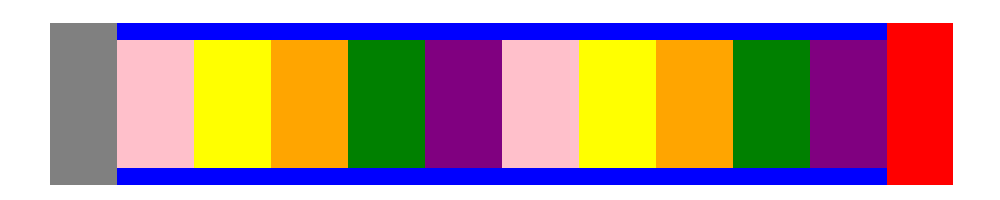
\includegraphics[width=\linewidth]{straightened_slab_mg.png}
    \raggedright
    \resizebox{0.5\textwidth}{!}{
        \hspace{1cm}
        \fbox{\begin{tabular}{llll}
            \textcolor{fhrblue}{$\blacksquare$} & FLiBe & 
            \textcolor{fhrgrey}{$\blacksquare$} & Left Graphite \\
            \textcolor{fhrred}{$\blacksquare$} & Right Graphite &
            \textcolor{fhrpink}{$\blacksquare$} & Fuel cell 1 $\&$ 6 \\
            \textcolor{fhryellow}{$\blacksquare$} & Fuel cell 2 $\&$ 7 &
            \textcolor{fhrorange}{$\blacksquare$} & Fuel cell 3 $\&$ 8 \\
            \textcolor{fhrgreen}{$\blacksquare$} & Fuel cell 4 $\&$ 9 &
            \textcolor{fhrpurple}{$\blacksquare$} & Fuel cell 5 $\&$ 10 \\
            \end{tabular}}}
    \caption{Straightened \acrfull{AHTR} fuel slab spatially discretized into 
    13 \textit{cells} for OpenMC multigroup calculation.}
    \label{fig:straightened_slab_mg}
\end{figure}
I used the four group energy structure derived by Gentry et al. 
\cite{gentry_development_2016} for \gls{AHTR} geometries. 
Table \ref{tab:energy_structures} defines the group boundaries. 
\begin{table}[H]
    \centering
    \onehalfspacing
    \caption{4-group energy structures for \acrfull{AHTR} geometry 
    derived by \cite{gentry_development_2016}.}
	\label{tab:energy_structures}
    \footnotesize
    \begin{tabular}{lll}
    \hline
    \multicolumn{3}{c}{\textbf{Group Boundaries [MeV]}} \\ 
    \hline
    \textbf{Group $\#$}& \textbf{Upper Bound} & \textbf{Lower Bound}  \\
    \hline 
    1 & $2.0000\times 10^1$ & $9.1188\times 10^{-3}$ \\ 
    2 & $9.1188\times 10^{-3}$ & $2.9023\times 10^{-5}$\\
    3 & $2.9023\times 10^{-5}$ & $1.8554\times 10^{-6}$\\
    4 & $1.8554\times 10^{-6}$ & $1.0000\times 10^{-12}$\\
    \hline
    \end{tabular}
\end{table}

The Moltres AHTR Steady-State Temperature Model first solves for the neutronics 
in slab and uses that to solve for the temperature distribution in the slab 
for a defined power. 
The temperature model assumes conductive heat transfer throughout the domain 
and heat removal by uniform salt flow in the coolant region. 
These assumptions ignore flow and turbulent effects that would most likely be 
present. 
However, an in-depth AHTR Moltres model that includes turbulence model is 
out of scope for this dissertation. 

Equation \ref{eq:moltres-temp} describes Moltres' governing equation for temperature
\begin{align}
    \label{eq:moltres-temp}
    \rho c_p\frac{\partial T}{\partial t} &+ \nabla\cdot\left(\rho
        c_f \vec{u}\cdot T -k\nabla T\right) =  Q
\end{align} 
In the 2D cross-sectional AHTR Steady-State Temperature Model, I ignore the 
time-dependent and velocity-dependent terms since I am solving for steady-state 
and there is no moving fuel: 
\begin{align}
    - \nabla \cdot (k_i \nabla T) &= Q_i
\intertext{where:}
k_i &= \mbox{thermal conductivity of material i} \nonumber \\
T &= \mbox{temperature in the slab} \nonumber \\
Q_i &= \mbox{source or sink term in material i} \nonumber
\end{align} 
Equation \ref{eq:moltres-source-term} defines the fuel cells' fission source term.
\begin{align}
    \label{eq:moltres-source-term}
        Q_f &= \sum_{g=1}^G \epsilon_{f,g}\Sigma_{f,g}\phi_g
    \intertext{where} 
    Q_f &= \mbox{source term } [\frac{MeV}{cm^3s}] \nonumber \\
    G &= \mbox{number of discrete neutron energy groups, g } [-] \nonumber \\
    \epsilon_{f,g} &= \mbox{heat produced per fission from neutrons in group g} [MeV] \nonumber \\
    \Sigma_{f,g} &= \mbox{macroscopic cross section for fission due to neutrons in group g } [\frac{1}{cm}] \nonumber \\
    \phi_g &= \mbox{flux of neutrons in group g } [\frac{n}{cm^2s}]\nonumber
    \end{align}
The heat removal from the AHTR fuel slab in the coolant areas: 
\begin{align}
    Q &= h \cdot (T(\vec{r})-T_{ref})
\intertext{where:}
Q &= \mbox{heat removal rate for 1cm thin slice of AHTR slab [W/cm]} \nonumber \\
h &= \mbox{heat transfer coefficient } [\frac{W}{cm \cdot K}] \nonumber \\
T(\vec{r}) &= \mbox{temperature at point $\vec{r}$ [K]} \nonumber \\
T_{ref} &= \mbox{reference temperature [K]} \nonumber
\end{align}
Table \ref{tab:heat-exchanger-constants} shows the values used for 
reference temperature and heat transfer coefficient for the convective 
heat transfer process.
\begin{table}[H]
    \centering
    \onehalfspacing
    \caption{AHTR Fuel Slab's heat transfer constants.}
	\label{tab:heat-exchanger-constants}
    \footnotesize
    \begin{tabular}{llll}
    \hline 
    \textbf{Constant}& \textbf{Value}& \textbf{Units} & \textbf{Notes} \\
    \hline 
    h & 990 & $\frac{W}{cm \cdot K}$ & Calculated in Eq. \ref{eq:calc-htc} \\
    $T_{ref}$ & 923 & K & AHTR Inlet Temperature \\ %cite ahtr 923K inlet temp 
    \hline
    \end{tabular}
\end{table} 
I calculated the heat transfer coefficient ($h$) using Equation \ref{eq:calc-htc} 
for the 1cm-thick AHTR $\Delta z$ slice with the following assumptions: 
\begin{itemize}
    \item it generates a constant amount of power, all of which is removed 
    by the coolant
    \item heat removal occurs at the coolant areas
    \item temperature increase per 1cm slice is constant from the inlet to the 
    outlet 
\end{itemize} 
\begin{align}
    \label{eq:calc-htc}
    h &= \frac{P_{dz}}{A_{coolant}} \div \frac{T_{total}}{H} \\
      &= \frac{1456 W}{23.1cm \times 0.5cm \times 2} / (50 K / 550 cm) \nonumber \\
      &= 990 W cm^{-1}K^{-1} \nonumber 
\intertext{where:}
h &= \mbox{heat transfer coefficient } [\frac{W}{cm \cdot K}] \nonumber \\
P_{dz} &= \mbox{power produced in 1cm AHTR slab $\Delta z$ slice [$W$]}\nonumber \\
A_{coolant} &= \mbox{cross-sectional coolant area in AHTR slab [$cm^2$]} \nonumber \\
T_{total} &= \mbox{total temperature change from inlet to outlet [$K$]} \nonumber \\
H &= \mbox{AHTR height from inlet to outlet [cm]} \nonumber 
\end{align}

Figure \ref{fig:ahtr_constant_temp} shows the Moltres-generated temperature 
distribution with an average and maximum temperature of 1019K and 1128K, 
respectively.
\begin{figure}[H]
    \centering
    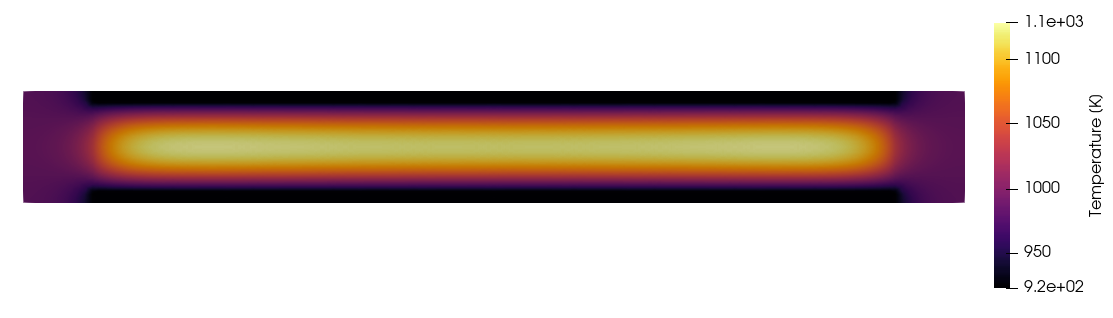
\includegraphics[width=\linewidth]{ahtr_constant_temp.png}
    \caption{AHTR fuel slab's Moltres generated temperature distribution for a 
    slab with a constant packing fraction of 0.0979 across ten fuel cells.}  
    \label{fig:ahtr_constant_temp}
\end{figure}
The temperature distribution is consistent with previous temperature models of 
the AHTR fuel slabs that report an average fuel kernel temperature of 1125K 
\cite{ramey_methodology_2021}. 
Model differences include that Ramey \cite{ramey_methodology_2021} utilized a 
1D temperature model with the original 4-layer TRISO model from the FHR benchmark 
(Figure \ref{fig:straightened_slab}).
This model is 2D and randomly disperses TRISO particles throughout the 
slab while keeping the same overall packing fraction. 

\section{FliBE Coolant Channel Shape Variation}
In the ROLLO optimization simulations, I vary the FliBE coolant channel shape 
while holding the total coolant area constant.  
Figure \ref{fig:ahtr-coolant-shape-variation} shows the example of how I intend 
to vary the channel shape while holding coolant area constant. 
\begin{figure}[H]
    \centering
    \begin{subfigure}{\textwidth}
        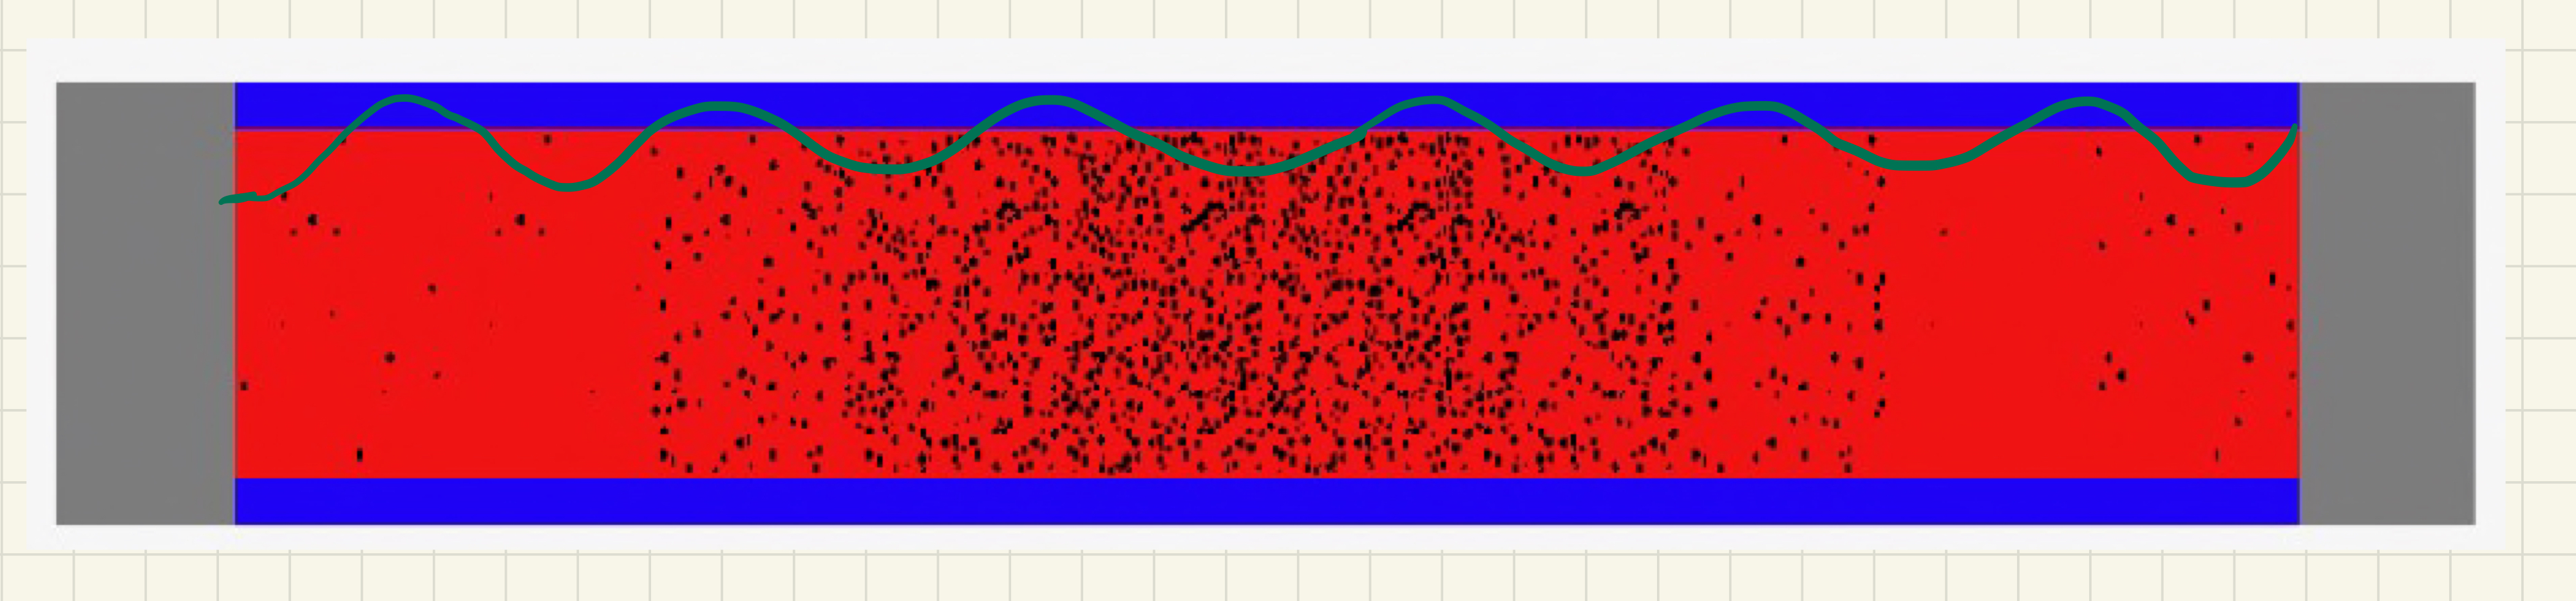
\includegraphics[width=\linewidth]{coolant_shape_variation_example.png}
        \caption{Example of where the coolant shape variation will occur.}
    \end{subfigure}
    \begin{subfigure}{\textwidth}
        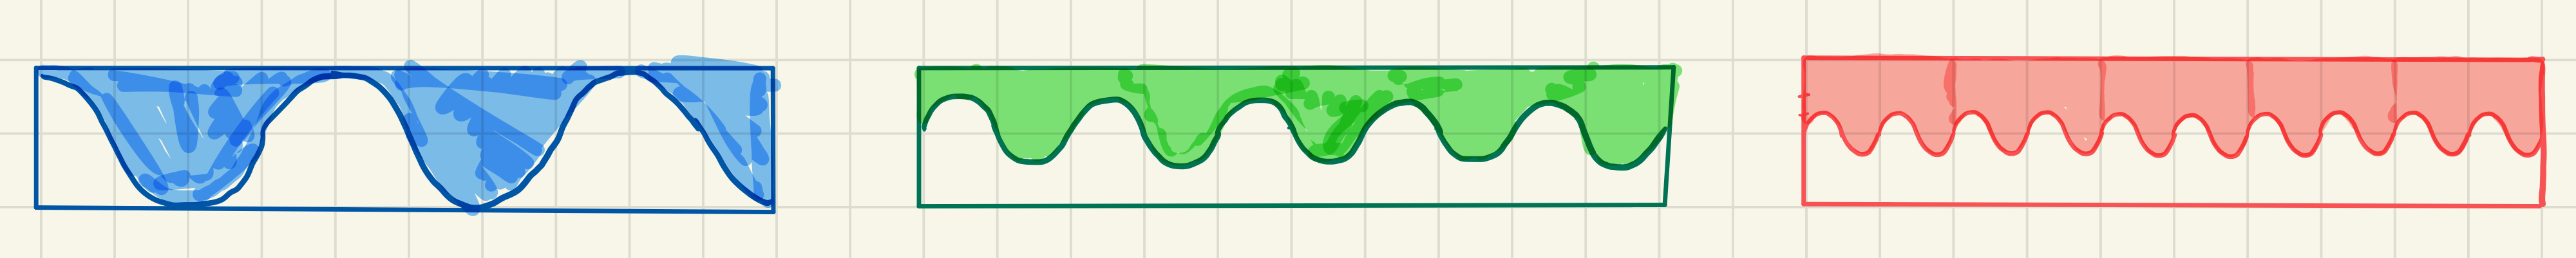
\includegraphics[width=\linewidth]{coolant_shape_variation.png}
        \caption{Specific examples of the coolant shape variations.}
    \end{subfigure}
    \caption{AHTR Coolant Shape Variation}  
    \label{fig:ahtr-coolant-shape-variation}
\end{figure}
Equation \ref{eq:calc-htc} calculated the heat transfer 
coefficient with the assumption that the slab generates a constant amount of power, 
and the heat removal occurs over the coolant areas.
Since the total coolant area is held constant, I use the 
same heat transfer coefficient ($h$) constant for all the simulations.   
%\chapter{Introduction}	
%\chapter{Literature Review}
\label{chap:lit-review}

This chapter provides a literature review of relevant past research efforts 
to give context to this dissertation. 
I begin with an overview of the \gls{FHR} concept, then detail one specific 
\gls{FHR} design: the \gls{AHTR}, previous efforts and technical 
challenges of modeling the design, and how these efforts led to the \gls{OECD} 
\gls{NEA}'s initiation of the \gls{FHR} benchmark.
Next, I outline additive manufacturing's history and describe the current 
research on applying additive manufacturing to the fabrication of nuclear 
reactor components. 
I review previous nuclear reactor design optimization efforts and describe how 
additive manufacturing of nuclear reactor components enables optimization for 
less constrained reactor geometries. 
I describe optimization methods, such as the evolutionary algorithm, that can 
be leveraged to find optimal reactor designs in the expanded design space.
Finally, I give a background of the evolutionary algorithms and detail a specific 
evolutionary algorithm: the genetic algorithm and how it works to conduct global 
optimization robustly.

\section{Fluoride-Salt-Cooled High-Temperature Reactor System}
\label{sec:fhr}
To ensure continued global use and expansion of nuclear energy technology, in 
2001, the \gls{OECD} and nuclear energy experts initiated the \gls{GIF} 
\cite{gif_technology_2002}.
The \gls{GIF} aims to enhance the role of nuclear energy in our global energy 
ecosystem by coordinating global research and development to test the 
feasibility and performance of Gen IV nuclear reactor systems, enabling 
their industrial deployment by 2030 \cite{gif_technology_2002}.
The \gls{GIF} selected six Generation IV systems for further research and 
development based on target goals in four areas: sustainability, 
economics, safety and reliability, and proliferation resistance and physical 
protection \cite{gif_technology_2002}. 
Table \ref{tab:goals-gen4} summarizes the goals in each area. 
\begin{table}[btp]
    \centering
    \onehalfspacing
    \caption{Goals of Generation IV Nuclear Systems \cite{gif_technology_2002,
    behar_technology_2014}}
	\label{tab:goals-gen4}
    \footnotesize
    \begin{tabular}{l|l}
    \hline
                               \textbf{Area} & \textbf{Goals} \\ \hline
    Sustainability   & - Have a positive impact on the environment through the displacement of \\
    & polluting energy and transportation sources by nuclear electricity generation \\
    & and nuclear-produced hydrogen \\ 
    & - Promote long-term availability of nuclear fuel \\
    & - Minimize volume, lifetime, and toxicity of nuclear waste \\ \hline
    Economics & - Have a life cycle and energy production cost advantage over other energy \\
    & sources \\ 
    & - Reduce economic risk to nuclear projects by developing plants using \\
    & innovative fabrication and construction techniques \\ \hline
    Safety and Reliability   & - Increase the use of robust designs and inherent and transparent safety\\
    & features that non-experts can understand \\ 
    & - Enhance public confidence in the safety of nuclear energy \\\hline
    Proliferation Resistance & - Provide continued effective proliferation resistance of nuclear energy \\
    and Physical Protection & systems through improved design features and other measures \\ 
    & - Increase the robustness of new facilities \\ \hline
    \end{tabular}
\end{table}
The systems are \glspl{GFR}, \glspl{LFR}, \glspl{MSR}, \glspl{SFR}, \glspl{SCWR}, 
and \glspl{VHTR} \cite{gif_technology_2002}. 
The \acrfull{FHR} concept introduced in 2003 uses a low-pressure liquid fluoride-salt 
coolant and high-temperature coated-particle \gls{TRISO} fuel, combining 
the best aspects of the \gls{MSR} and \gls{VHTR} systems respectively
\cite{forsberg_molten-salt-cooled_2003,facilitators_fluoride-salt-cooled_2013}.

\gls{MSR} systems produce fission power in a circulating molten salt fuel 
mixture. 
Researchers recommend molten fluoride salts because they have high uranium 
solubility, chemical stability, low vapor pressure at high temperatures, 
good heat transfer properties, radiation damage resistance, and are inert 
to common structural materials \cite{rosenthal_molten-salt_1970}. 
Molten salt reactor coolants also introduce inherent safety due to the 
low system vapor pressure and the salts' high boiling temperature and 
volumetric heat capacity \cite{ho_molten_2013}.
Fluoride salt used in \glspl{FHR} is Li$_2$BeF$_4$ (FLiBe), 
which remains liquid without pressurization up to 1400 $^{\circ}$C and has a greater 
heat capacity than water \cite{ho_molten_2013,forsberg_fluoride-salt-cooled_2012}.
\gls{VHTR} systems use a once-through uranium cycle and leverage 
high outlet temperatures for high-temperature heat applications, such as 
hydrogen production. 
Graphite-moderated and helium-cooled \glspl{VHTR} use \gls{TRISO} fuel
which withstands high burnup and temperature, enabling higher operating 
temperatures \cite{gif_technology_2002}.  
Higher operating temperatures advantages include increased power 
conversion efficiency, reduced waste heat generation, and co-generation and 
process heat capabilities \cite{scarlat_design_2014}.
However, the \glspl{VHTR} system's helium coolant is at 100 atm requiring a 
thick concrete vessel. 

By combining the FLiBE coolant from \gls{MSR} technology and 
\gls{TRISO} fuel from \gls{VHTR} technology, the \gls{FHR} benefits from 
low operating pressure and big thermal margin enabled by the molten 
salt coolant and the thermal resilience of \gls{TRISO} particle fuel. 
Molten salt coolant has superior cooling properties. Molten salt coolant 
increases system safety with an atmospheric operating pressure compared to 
\gls{VHTR}'s 100 atm. 
\gls{TRISO} solid fuel cladding in the \gls{FHR} system adds an extra barrier 
to fission product release compared to \glspl{MSR} with liquid fuel 
\cite{ho_molten_2013}.

Several types of \gls{FHR} conceptual designs exist worldwide: the \gls{PBFHR} 
developed at \gls{UCB} with circulating pebble-fuel 
\cite{scarlat_current_2014,krumwiede_three-dimensional_2013}, the \gls{SF-TMSR} 
developed at the \gls{SINAP} in China with static pebble-fuel \cite{liu_preliminary_2016}, 
the large central-station \gls{AHTR} at \gls{ORNL} \cite{holcomb_core_2011, varma_ahtr_2012}, 
and the \gls{SmAHTR} at ORNL \cite{greene_pre-conceptual_2010} with static, 
plate fuel. 

\subsection{\acrlong{AHTR} Design}
This dissertation focuses on the prismatic \gls{FHR} design with hexagonal fuel 
assemblies consisting of \gls{TRISO} fuel particles embedded in planks, i.e., 
the \gls{AHTR} design developed by ORNL. 
The \gls{AHTR} has 3400 MWt thermal power and 1400 MW electric power with
inlet/outlet temperatures of 650/700$^{\circ}$C \cite{varma_ahtr_2012}.  
Figure \ref{fig:ahtr} shows the prismatic AHTR's fuel assembly and core 
configuration.  
\begin{figure}[btp]
    \centering
    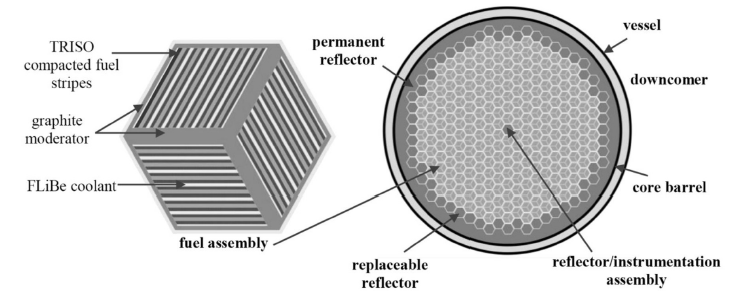
\includegraphics[width=\linewidth]{ahtr.png} 
    \caption{\acrlong{AHTR} fuel assembly (left) and core configuration (right) 
    reproduced from \cite{ramey_monte_2018}.}
    \label{fig:ahtr}
\end{figure}
Each hexagonal fuel assembly features plate-type fuel consisting of eighteen 
planks arranged in three diamond-shaped sectors, with a central Y-shaped 
structure and external channel (wrapper).
The fuel planks contain an isostatically pressed carbon with fuel stripes 
on each plank's outer side.
Within each fuel stripe is a graphite matrix filled with \gls{TRISO} particles. 
The core consists of 252 assemblies radially surrounded by reflectors
\cite{ramey_monte_2018}. 
Chapter \ref{chap:fhr-benchmark} details the specifications of the AHTR geometry
modeled in this proposed work.

\subsection{Previous AHTR modeling efforts and challenges} 
\label{sec:previous_ahtr}
The \gls{AHTR} core design differs significantly from the present \gls{LWR} 
systems' cores. 
These differences lead to modeling challenges with the current tools, 
highlighting the need to verify and validate current simulation tools
for \gls{AHTR} physics \cite{ramey_monte_2018}. 
Verification and validation of \gls{AHTR} neutronics and thermal-hydraulics 
simulation capabilities support the \gls{AHTR} design's licensure and the
eventual goal of \gls{AHTR} deployment 
\cite{rahnema_phenomena_2019,rahnema_current_2015}.
This section outlines the previous efforts taken to model and validate 
the \gls{AHTR}'s neutronics and thermal-hydraulics. 

\subsubsection{AHTR Neutronics Modeling}
Several neutronics studies conducted along the way to the current \gls{AHTR} 
design have shed light on the design's technical challenges 
\cite{ramey_monte_2018,holcomb_fluoride_2013,greene_pre-conceptual_2010}. 
\gls{Georgia Tech} led an Integrated Research Project to understand \gls{AHTR} 
material and modeling challengess \cite{zhang_integrated_2019}. 
During the research project, a panel of subject matter experts 
generated a \gls{PIRT}.
The \gls{PIRT} identifies areas that need additional research to better 
understand important phenomena for adequate future modeling
\cite{rahnema_phenomena_2019}. 
Table \ref{tab:phenomena} lists the phenomena identified as requiring further 
research. 
\begin{table}[btp]
    \centering
    \onehalfspacing
    \caption{\acrlong{PIRT} identified \acrlong{AHTR} physical phenomena requiring 
    further research \cite{rahnema_phenomena_2019}.}
	\label{tab:phenomena}
    \footnotesize
    \begin{tabular}{l|l}
    \hline
    \textbf{Category} & \textbf{Phenomena} \\ \hline
    Fundamental cross section data & - Moderation in FliBe \\
    & - Thermalization in FliBe \\
    & - Absorption in FliBe \\
    & - Thermalization in carbon \\
    & - Absorption in carbon \\ \hline
    Material Composition & - Fuel particle distribution \\ \hline
    Computational Methodology & - Solution Convergence \\ 
    & - Granularity of depletion regions \\
    & - Multiple heterogeneity treatment for generating multigroup \\ 
    & cross sections \\
    & - Selection of multigroup structure \\
    & - Boundary conditions for multigroup cross section generation \\ \hline 
    General Depletion & - Spectral history \\ \hline 
    \end{tabular}
\end{table}

The \emph{triple heterogeneous} \gls{AHTR} fuel, comprised of \gls{TRISO} 
particles embedded in strategically arranged plates, presents simulation 
challenges. 
Researchers must obtain detailed reference power distributions with individual 
\gls{TRISO} particle fidelity to understand nuances in the physics, such 
as self-shielding.
Deterministic codes that use multigroup cross sections and traditional 
homogenization methods \cite{ramey_monte_2018}, insufficiently capture the 
\glspl{AHTR} physics due to these multiple heterogeneities 
\cite{ramey_monte_2018}. 
In the \gls{AHTR}, single and multiple slab homogenization decreased total 
neutron transport simulation time by an order of 10; however, the homogenization 
introduced a nontrivial $k_{eff}$ error of $\sim$3\% 
\cite{ramey_monte_2018,cisneros_neutronics_2012}.
To determine the feasibility and safety of the \gls{AHTR} design, researchers 
must calculate core physics parameters to an acceptable uncertainty. 
With Monte Carlo neutron transport, increasing neutron histories reduces statistical 
uncertainty but increases computational cost typically, requiring
supercomputers to run the simulations.

This \gls{AHTR} presents another technical challenge: the uncertainty of 
graphite moderator material properties: densities, temperatures, and thermal 
scattering data.
Also, the thermal scattering data ($S(\alpha,\beta)$ matrices) for 
the bound nuclei in \gls{FLiBe} salts are lacking \cite{ramey_monte_2018}. 
Mei et al. \cite{mei_investigation_2013} and Zhu et al. \cite{zhu_thermal_2017} 
examined the thermal scattering behavior of solid and liquid \gls{FLiBe}.
They concluded that the bound and free atom cross section of \gls{FLiBe} are 
identical above 0.1eV and diverge below 0.01eV, which means that the use or 
absence of thermal scattering data will impact the accuracy of the results 
\cite{ramey_monte_2018}. 

\subsubsection{AHTR Multiphysics Modeling}
In past effort toward \gls{AHTR} multiphysics modeling, Gentry et al. 
\cite{gentry_development_2016} developed an adapted lattice physics-to-core 
simulator two-step procedure with Serpent \cite{leppanen_serpent_2014} 
and \gls{NESTLE} \cite{turinsky_nestle_1994} for the \gls{AHTR} design. 
The adapted lattice physics-to-core simulator two-step procedure proved to be 
successful for \glspl{LWR}. A 2-D transport lattice calculation generates the 
\gls{LWR}'s group assembly homogenized group constants, and then core 
analysis is performed by 3-D nodal simulation 
\cite{koebke_new_1980,gentry_development_2016}.
\gls{NESTLE}'s thermal-hydraulics utilizes a \gls{HEM} model for two-phase 
flow, and it solves the few-group neutron diffusion equation utilizing the
\gls{NEM} for cartesian and hexagonal reactor geometries.  
Gentry et al. concluded that the method required accuracy improvements 
by improving the reflector model and further optimizing the coarse energy group 
structure.
Lin \cite{lin_thermal_2020} used RELAP5, a system-level code, to perform 
\gls{AHTR} thermal hydraulics transient simulations to investigate the 
capability of the passive heat removal system. 
In the RELAP5 model, Lin separated the \gls{AHTR}'s 252 assemblies into 
four concentric rings with uniform power distribution per ring. 
Lin also gives higher fidelity in the primary and \gls{DRACS} system loops. 
Lin utilized RELAP5 in transient scenarios to determine 
the temperature at various locations in the system loop by assuming a power 
value for fuel assemblies in each ring \cite{lin_thermal_2020}. 
However, this method is not ideal for transient scenarios with tightly coupled 
neutronics and thermal-hydraulics. 

\subsection{FHR Benchmark}
The previous section highlights the singular efforts to model 
different aspects of the \gls{AHTR}'s neutronics and thermal hydraulics, with
each author describing their modeling difficulties. 
However, there lacked a robust and methodical method for evaluating the 
simulation software and comparing the \gls{AHTR} modeling results generated by 
individual researchers.

To gain a comprehensive view of the \gls{AHTR}'s modeling challenges and 
cross-verify available \gls{AHTR} modeling tools, in 2019, the 
\gls{OECD}-\gls{NEA} initiated the \gls{FHR} benchmarking exercise 
of the \gls{AHTR} design \cite{noauthor_fluoride_nodate}.
Several organizations participate in the benchmark with various Monte Carlo
and Deterministic neutronics software, such as Serpent \cite{leppanen_serpent_2014}, 
OpenMC \cite{romano_openmc_2013}, and WIMS \cite{lindley_current_2017}. 

The benchmark has three phases: a single fuel assembly simulation 
without burnup (Phase I), full core depletion (Phase II), and multiphysics 
feedback (Phase III). 
The benchmark aims to identify the latest codes' applicability, accuracy, 
and practicality to assess the current state-of-the-art FHR simulation 
and modeling \cite{petrovic_preliminary_2021}. 
The benchmark also enables the cross-verification of software and methods 
for the challenging \gls{AHTR} geometry, which is especially useful since 
applicable reactor physics experiments for code validation are scarce 
\cite{petrovic_fhrahtr_2019,petrovic_preliminary_2021}. 
Chapter \ref{chap:fhr-benchmark} will provide a detailed description of the 
benchmark phases and results.

\subsection{Modeling Software}
\label{sec:lit-review-modeling-software}
In this dissertation, I use OpenMC \cite{romano_openmc:_2015} to model \gls{AHTR}'s 
neutronics and Moltres \cite{lindsay_introduction_2018} to model the \gls{AHTR}'s 
multiphysics. 
OpenMC is an open-source Monte Carlo neutron transport code capable of 
performing k-eigenvalue calculations on models built using either constructive 
solid geometry or CAD representation. 
OpenMC supports both continuous-energy and multigroup transport.
A hybrid MPI and OpenMP programming model enables OpenMC's parallelism
\cite{romano_openmc:_2015}.

Moltres is an open-source tool designed to simulate \glspl{MSR} using 
deterministic neutronics and thermal-hydraulics implemented as an application 
atop the \gls{MOOSE} finite-element framework.  
Moltres solves arbitrary group neutron diffusion, temperature, and precursor 
governing equations on a single mesh and can be deployed on an arbitrary number 
of processing units \cite{lindsay_introduction_2018}.
Moltres solves the diffusion equations as a steady-state eigenvalue 
problem to find $k_{eff}$ for the static AHTR model: 
\begin{align}
    \label{eq:moltres-diffusion-equation}
    \frac{1}{v_g} \frac{\partial \phi_g}{\partial t} &= \nabla \cdot D_g
    \nabla \phi_g - \Sigma^r_g \phi_g +
    \sum^G_{g' \neq g} \Sigma^s_{g' \rightarrow g} \phi_{g'} + \chi^p_g
    \sum^G_{g'=1} (1-\beta) \nu \Sigma^f_{g'} \phi_{g'} + \chi^d_g \sum^I_i
    \lambda_i C_i
\end{align}

Equation \ref{eq:moltres-temp} describes Moltres' governing equation for temperature:
\begin{align}
    \label{eq:moltres-temp}
    \rho c_p\frac{\partial T}{\partial t} &+ \nabla\cdot\left(\rho
        c_f \vec{u}\cdot T -k\nabla T\right) =  Q
\end{align} 

\section{Additive Manufacturing}
Additive manufacturing is the formal term for what is popularly known as `3D printing' 
\cite{gibson_additive_2014}. 
The basic principle of additive manufacturing is that a model is initially generated using a
\gls{3D CAD} system and then fabricated directly without process planning. 
As the name implies, additive manufacturing adds material in layers. 
Each layer is a thin cross section of a \gls{3D CAD}-designed part, as opposed 
to traditional machining, which subtracts material instead 
\cite{standard_standard_2012}. 
All commercialized additive manufacturing machines to date use a layer-based 
approach.
The major ways they differ are in materials, layer creation method, and 
how the layers are bonded \cite{gibson_additive_2014}.
These major differences will determine the: accuracy of the 
final part, material and mechanical properties, time required to manufacture 
the part, need for post-processing, size of additive manufacturing machine, and overall 
cost of the machine and the process \cite{gibson_additive_2014}. 
Initially, industries only utilized additive manufacturing for manufacturing 
prototypes. 
However, with improvements in material properties, accuracy, and overall 
quality of additive manufacturing output, the applications for additive 
manufacturing have advanced. 
Industries have begun 3D printing parts for direct assembly purposes, 
such as air-cooling ducts for aircraft, hearing aids, and prosthesis
\cite{uriondo_present_2015}.  

Additive manufacturing has progressed rapidly in the last 30 years, from rapid 
design prototyping with polymers in the automotive industry to scale production 
of metal components.  
Examples include Boeing using additive manufacturing to reduce the 979 
Dreamliner's weight \cite{noauthor_printed_2017} and General Electric using 
additive manufacturing to produce fuel injection nozzles 
\cite{noauthor_transformation_2018}. 
The most common metal additive manufacturing technologies, \gls{SLM}, \gls{EBM}, 
\gls{L-DED}, and binder jetting, are not currently used to manufacture nuclear 
power plant parts. 

The U.S. \gls{DOE}, National Laboratories, and \gls{EPRI} support research and 
development efforts toward deploying, testing, and qualifying additive 
manufacturing methods for nuclear components. 
However, the nuclear industry's efforts to incorporate additive manufacturing 
into the supply chain lag behind the auto and aerospace industries due to the 
lack of clarity on regulatory pathways. 
The aerospace and automotive industries benefit from long-standing and resourced 
regulatory and standards development activities \cite{noauthor_roadmap_nodate}. 
Thus, in 2019 the \gls{NRC} addressed these regulatory challenges by issuing 
a draft action plan to prepare the agency to review applications for 
additive manufacturing of nuclear components and clarify the industry's 
expectations of their use \cite{noauthor_roadmap_nodate}.

\subsection{Benefits of 3D Printing Reactor Components}
\label{sec:am}
Wide-spread adoption of additive manufacturing methods in the nuclear industry 
could drastically reduce fabrication costs and timelines.
These reductions are achieved by combining multiple systems and assembled 
components into single parts, tailoring local material properties, and enabling 
geometry redesign for increased safety and performance 
\cite{simpson_considerations_2019}. 
Many Generation IV advanced reactor concepts have complex geometries, 
such as hex-ducts for sodium-cooled fast reactors, that are costly and difficult 
to fabricate using standard processing techniques \cite{sridharan_performance_2019}.  
These complex designs will benefit from 3D printed parts. 
Additive manufacturing advancements for reactor core components remove
conventional fuel manufacturing geometric constraints.
Reactor designers can now approach the nuclear design problems with truly 
arbitrary geometries, no longer limited by traditional geometric shapes that are 
easy to manufacture with traditional processes: slabs as fuel planks, cylinders 
as fuel rods, spheres as fuel pebbles, axis-aligned coolant channels, etc 
\cite{sobes_artificial_2020}.
In summary, reactor core component fabrication with additive manufacturing 
enables further fuel geometry optimization and improvement to enhance 
reactor performance at lower costs \cite{bergeron_early_2018}. 

\subsection{Efforts toward 3D Printing Reactor Components}
In 2019, \gls{ORNL} initiated the \gls{TCR} Demonstration Program.
The \gls{TCR} program leverages recent scientific achievements in additive 
manufacturing, nuclear materials, machine learning, and computational modeling
to reduce deployment costs and timelines for advanced nuclear energy systems. 
The \gls{TCR} program aims to utilize additive manufacturing technology to 
establish advanced nuclear energy system designs unconstrained by conventional 
manufacturingand build an additively manufactured microreactor 
\cite{terrani_transformational_2019}. 

The \gls{TCR} program followed a downselection process based on the program's 
design constraints to select the reactor's design, materials, and components
\cite{betzler_transformational_2020}.
The downselected TCR design is a TRISO-fueled and yttrium hydride moderated 
gas-cooled reactor \cite{betzler_transformational_2020}.
At \gls{ORNL}, Trammel et al. \cite{trammell_advanced_2019} demonstrated 
the fabrication of a SiC fuel element with embedded \gls{TRISO} fuel using 
additive manufacturing techniques: binder jet printing and \gls{CVI}. 
They followed the following fabrication steps (depicted in Figure 
\ref{fig:ornl-triso-print}): 
\begin{enumerate}
    \item Binder jet technology prints a SiC fuel element with coolant channel 
    structures. 
    \item The designated fueled region of the element is loaded with surrogate 
    \gls{TRISO} particles and additional SiC powder to fill interstitial spaces
    between particles. 
    \item The loaded fuel element is densified in a \gls{CVI} process to achieve 
    microencapsulation of \gls{TRISO} particles in a SiC matrix. 
\end{enumerate}
\begin{figure}[btp]
    \centering
    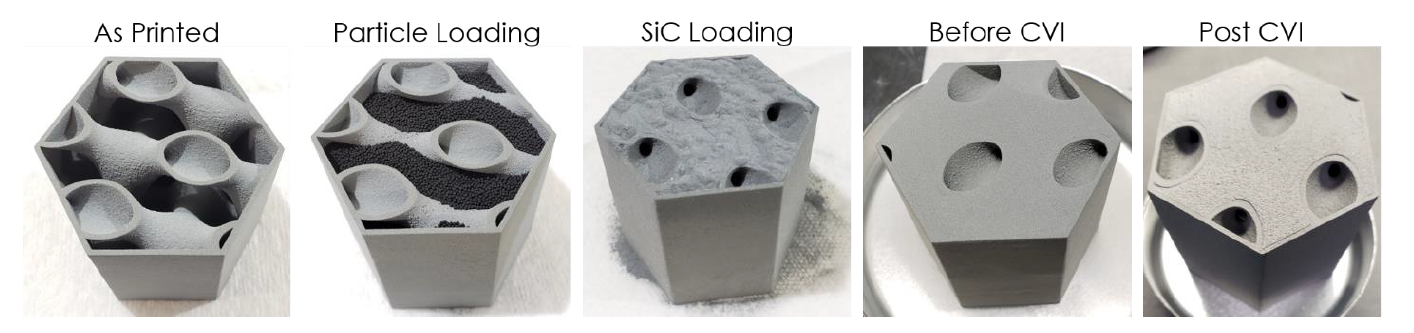
\includegraphics[width=\linewidth]{ornl-triso-print.png} 
    \caption{Stages of additive manufacturing fabrication conducted at \acrlong{ORNL} to 
    produce a fuel demonstration element with \gls{TRISO} particles embedded in 
    a SiC matrix \cite{trammell_advanced_2019}. Figure reproduced from 
    \cite{trammell_advanced_2019}.}
    \label{fig:ornl-triso-print}
\end{figure}
Figure \ref{fig:ornl-fuel-element} shows the the fuel element manufactured at 
\gls{ORNL} for the \gls{TCR} program \cite{betzler_transformational_2020}. 
\begin{figure}[btp]
    \centering
    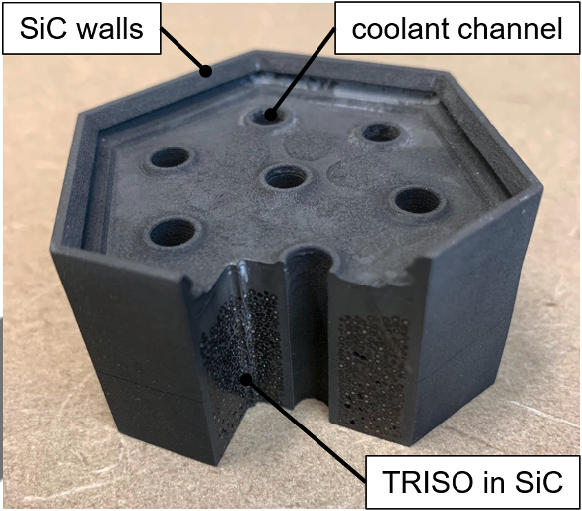
\includegraphics[width=0.6\linewidth]{ornl-fuel-element.png} 
    \caption{The top portion of the advanced manufactured fuel element 
    reproduced from \cite{betzler_transformational_2020} for the \acrfull{TCR} 
    program at \acrfull{ORNL}. A cutaway of the element shows surrogate TRISO 
    particles packed in the SiC matrix.}
    \label{fig:ornl-fuel-element}
\end{figure}
The current design uses fuel shapes and coolant channels that are uniform in the 
axial dimension. 
The \gls{TCR} program plans to optimize the coolant channels to vary in axial 
and radial directions within the fuel element 
\cite{betzler_transformational_2020,sobes_artificial_2020}. 

Besides the \gls{TCR} program, the nuclear materials research community has made 
significant progress in demonstrating the application of additive manufacturing 
to nuclear fuel and structural core material fabrication. 
Rosales et al. \cite{rosales_characterizing_2019} conducted a feasibility study 
of direct routes to fabricate dense uranium silicide (U$_3$Si$_2$) fuel pellets 
using the \gls{INL} approach known as \gls{AMAFT}. 
U$_3$Si$_2$ demonstrates desirable accident-tolerant nuclear fuel properties 
such as high uranium density and improved thermal properties; however, it has 
an expensive and long metallurgical fabrication process. 
Thus, using \gls{AMAFT} to fabricate U$_3$Si$_2$ will lower costs and ensure a
timely and commercially-reliable fabrication process \cite{rosales_characterizing_2019}. 
Sridharan et al. \cite{sridharan_performance_2019} demonstrated applying
the laser-blown-powder additive manufacturing process to fabricate \gls{FM} steel, 
a type of steel commonly used for cladding and structural components in nuclear 
reactors. 
Koyanagi et al. \cite{koyanagi_additive_2020} presented the latest 
additive manufacturing technology for manufacturing nuclear-grade \gls{SiC} materials. 
They demonstrated that combinations of additive manufacturing techniques and 
traditional \gls{SiC} densification methods enabled new designs of \gls{SiC} 
components with complex shapes. 
\gls{SiC} demonstrates excellent strength at elevated temperatures, chemical inertness, 
relatively low neutron absorption, and stability under neutron irradiation up 
to high doses \cite{sauder_ceramic_2014, snead_handbook_2007,koyanagi_additive_2020}. 
These qualities make \gls{SiC} suitable for many applications in nuclear systems, 
such as fuel cladding, constituents of fuel particles \cite{snead_handbook_2007} 
and pellets \cite{terrani_progress_2015}, and core structural components in fission 
reactors \cite{sauder_ceramic_2014}. 

% Advancements of nuclear material additive manufacturing technology 
% will enable 3D printing of nuclear reactors which will reduce the cost 
% and fabrication timelines. 

% The TCR Program's prototype demonstration of 3D printing a reactor shows promise 
% for the field.  

%Many of the materials and fabrication methods discussed above are applicable 
%for \gls{FHR}-part manufacturing. 
%Therefore, this reiterates the possibility of leveraging additive manufacturing 
%to 3D print a \gls{FHR}-type reactor with non-conventional geometry. 

\section{Nuclear Reactor Design Optimization}
\label{sec:opt}
A nuclear reactor's complexity results in reactor design optimization being a 
multi-objective design problem requiring a tradeoff between desirable 
attributes \cite{byrne_evolving_2014,simon_sciences_2019}. 
When multiple conflicting objectives compete, no single optimum solution 
simultaneously optimizes all objectives. 
Instead, multi-objective optimization returns multiple optimal 
solutions that meet each objective to varying degrees; this set of solutions is 
the Pareto front \cite{deb_multi-objective_2001}. 
For each solution in the Pareto front, none of the objective functions can be 
improved without degrading another objective.
An ideal optimization method for a multi-objective problem like reactor design 
should find widely spread solutions in the obtained Pareto front 
\cite{deb_multi-objective_2001}. 

Traditional manufacturing constraints result in most of past nuclear reactor 
optimization work focusing on optimizing classical reactor 
parameters such as radius of fuel pellet and clad, enrichment of fuel, 
pin pitch, etc. 
The optimization methods used for reactor design optimization are either 
deterministic or stochastic. 
Deterministic optimization methods usually start from a guess solution.
Then, the algorithm suggests a search direction by applying local 
information to a pre-specified transition rule. 
Any better solution becomes the new solution, and the above procedure continues 
several times \cite{deb_multi-objective_2001}. 
Drawbacks of deterministic methods include: algorithms tend to get stuck at
suboptimal solutions, and an algorithm efficient in solving one type of problem 
may not solve a different problem efficiently \cite{deb_multi-objective_2001}. 
Stochastic optimization methods such as evolutionary algorithms and simulated annealing
minimize or maximize an objective function with randomness present. 
Stochasticity enables them to find globally optimal solutions more reliably than 
deterministic methods. 
Due to stochastic methods' many advantages, most efforts toward nuclear 
reactor optimization use these methods. 

In recent years, additive manufacturing advancements for reactor core components 
removed conventional reactor manufacturing geometric constraints such as slabs as fuel 
planks, cylinders as fuel rods, spheres as fuel pebbles, axis-aligned coolant 
channels, etc  \cite{sobes_artificial_2020}.
Reactor design objectives remain consistent with past objectives, such as 
minimizing fuel amount and minimizing the maximum fuel temperature for a given 
power level.
However, reactor designers can now approach nuclear design problems with truly 
arbitrary geometries and optimize beyond classical parameters to further enhance 
fuel performance and safety.
This has opened the door for a re-examination of reactor core 
optimization completely, determining the optimal arbitrary geometry 
and fuel distribution for a given objective function with a much smaller set of 
constraints \cite{sobes_artificial_2020}. 

In the subsequent sections, I discuss the previous nuclear reactor optimization 
efforts for classical and arbitrary parameters.

\subsection{Reactor Optimization for Classical Parameters}
The most commonly used stochastic optimization methods for reactor design 
optimization are simulated annealing and evolutionary algorithms. 

\subsubsection{Reactor Optimization with Simulated Annealing Method}
Simulated annealing iteratively updates one candidate solution until it reaches 
the termination criteria. 
At each iteration, the simulated annealing algorithm selects a random move. 
If the selected move improves the solution, it is always accepted; however,  
if it does not improve the solution, the algorithm updates the solution with 
some probability of less than 1.

Sacco et al. \cite{sacco_two_2006,sacco_metropolis_2008} used stochastic 
simulated annealing and deterministic-stochastic hybrid optimization techniques 
to optimize reactor dimensions, enrichment, materials, etc., to 
minimize the average peaking factor in a three-enrichment-zone reactor. 
Odeh et al. \cite{odeh_core_2016} used the simulated annealing stochastic algorithm 
coupled with neutronics and thermal-hydraulics simulation tools, \gls{PARCS} and RELAP5
\cite{fletcher_relap5mod3_1992}, to develop an optimal \gls{NMR-50} core design 
with a 10-year cycle length and minimal fissile loading. 
Kropaczek et al. \cite{kropaczek_large-scale_2019} demonstrated the constraint 
annealing method: a highly scalable method based on the parallel simulated annealing 
method with mixing of states \cite{kropaczek_constraint_2019} to solve large-scale, 
multiconstrained problems in \gls{LWR} fuel cycle optimization. 
These papers demonstrate the simulated annealing optimization method's success in 
reactor design optimization problems. 

Nuclear reactor optimization problems require computationally 
expensive neutronics and thermal-hydraulics software to compute the objective 
function and constraints. 
Multiple papers utilized stochastic optimization methods with surrogate models 
to reduce computational cost. 
The surrogate models reduce the computational cost by replacing high-fidelity
neutronics or thermal hydraulics simulations.
Betzler et al. \cite{betzler_design_2019} developed a systematic approach to 
build a surrogate model to serve in place of high-fidelity computational 
analyses. 
They leveraged the surrogate model with a simulated annealing optimization 
algorithm to generate optimized designs at a lower computational cost and
understand the impact of design decisions on desired metrics for \gls{HFIR} \gls{LEU} 
core designs.

The simulated annealing method uses a point-by-point approach:
one solution gets updated to a new solution in one iteration, which does not 
exploit parallel systems' advantages.
Finding an optimal solution with simulated annealing methods takes very long if 
high-fidelity computationally expensive codes compute the objective function and 
constraints.
Using a simulated annealing method is only practical with surrogate evaluation models, 
as described in Betzler et al. \cite{betzler_design_2019}.

\subsubsection{Reactor Optimization with Evolutionary Algorithm Method}
Contrary to a single solution per iteration in deterministic and stochastic 
simulated annealing methods, evolutionary algorithms use a population of 
solutions in each iteration \cite{deb_multi-objective_2001}. 
Evolutionary algorithm methods mimic nature's evolutionary principles by driving 
the search toward an optimal solution.

Peireira et al. \cite{pereira_coarse-grained_2003,pereira_parallel_2008} 
used a coarse-grained parallel genetic algorithm and a niching genetic algorithm
to minimize the average peaking factor in a three-enrichment-zone reactor. 
Kamalpour et al. \cite{kamalpour_smart_2020} utilized the imperialist competitive 
algorithm, an evolutionary algorithm, to optimize an \gls{FCM} fuelled 
\gls{PWR} to extend the reactor core cycle length. 
Kumar et al. \cite{kumar_new_2015} combined genetic algorithm optimization 
with a surrogate model to optimize for high breeding of $^{233}$U and $^{239}$Pu 
in desired power peaking limits and keff by varying: fuel pin 
radius,  fissile material isotopic enrichment, coolant mass flow rate, and 
core inlet coolant temperature.

With the affordability and availability of parallel computing systems, the 
evolutionary algorithm optimization method stands out as a method 
that easily and conveniently exploits parallel systems. 
Further, evolutionary algorithms have proved amenable to \gls{HPC} solutions and 
scalable to tens of thousands of processors \cite{kropaczek_constraint_2019}. 
Thus, for optimization problems that require high-fidelity evaluation software, 
the evolutionary algorithm method can leverage parallel computing to find a 
solution faster than the simulated annealing method.
herefore, I will utilize the evolutionary algorithm optimization method in 
this dissertation.
Section \ref{sec:ea} gives a literature review on evolutionary algorithms.

\subsection{Reactor Optimization for Arbitrary Parameters}
\label{sec:lit-review-reactor-arbitrary}
Sobes et al. \cite{sobes_artificial_2020} used a genetic algorithm to find 
minimum volume geometric configurations for a \gls{TCR}-like reactor with 
multiphysics constraints of 1500 pcm excess reactivity and maximum fuel 
temperature of 618 $^{\circ}C$ under forced-flow cooling conditions. 
They constrained the solution geometry to right cylinders to represent 
arbitrary geometry variation.
The authors acknowledge that this work is only a first step towards truly 
arbitrary geometry expression. 
They found that the optimal cone-like core configuration is in the geometry 
shape of a truncated annular cone, with the inlet surface being larger than 
the outlet \cite{sobes_artificial_2020}.

See et al. \cite{see_design_2022} conducted design optimization of the 
\gls{TCR}'s outlet plenum design with Siemens design optimization tool HEEDS
and \gls{CFD} code, STAR-CCM+. 
They had to design an instrumentation plane to monitor core coolant flow average 
temperature within $\pm 5 ^{\circ}C$ while maintaining a tight design 
constraint of 0.5-psi pressure drop across the outlet plenum.
The optimal design maintained a pressure drop to 0.49 psi with an instrumentation 
plane temperature standard deviation of $1.03^{\circ}C$. 
Figure xx shows the initial and optimal outlet plenum designs. 
Figure \ref{fig:see3} demonstrates how the optimal design impacted the stream 
tubes and enabled a smaller temperature standard deviation in the 
instrumentation plane. 
\begin{figure}[btp]
    \centering
    \begin{subfigure}{0.49\textwidth}
        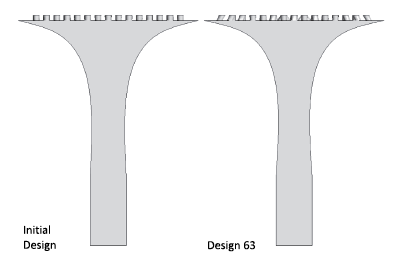
\includegraphics[width=\linewidth]{see1.png}
        \caption{Geometric representation of outer wall spline.}
        \label{fig:see1} 
    \end{subfigure}
    \begin{subfigure}{0.49\textwidth}
        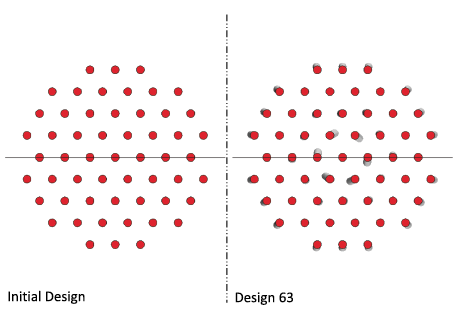
\includegraphics[width=\linewidth]{see2.png}
        \caption{Geometric representation of inlet channels.}
        \label{fig:see2} 
    \end{subfigure}
    \caption{Initial design versus the best design of outlet plenum, reproduced 
    from \cite{see_design_2022}.}
\end{figure}
\begin{figure}[btp]
    \centering
    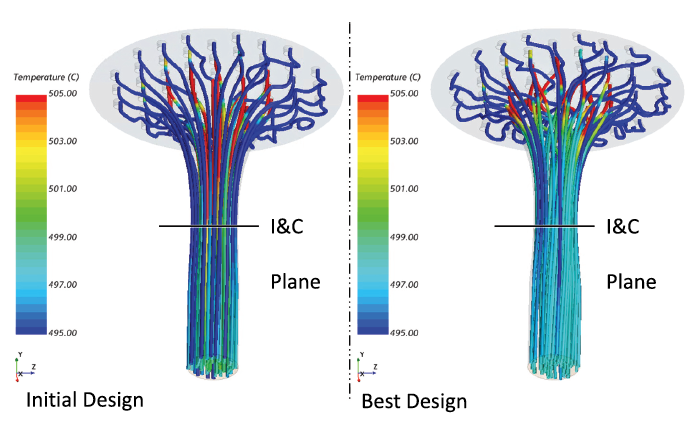
\includegraphics[width=0.8\linewidth]{see3.png} 
    \caption{Initial design versus best design of stream tubes in the outlet 
    plenum, reproduced from \cite{see_design_2022}.}
    \label{fig:see3}
\end{figure}

Reactor optimization for arbitrary parameters is a new concept, and only a few 
research demonstrations have begun exploring the large new design space. 
As additive manufacturing technology advances and the \gls{TCR} program 
demonstrates the first 3D printed operational reactor, more reactor designers 
will begin to explore the huge design space enabled by 3D printing. 
To fully explore the design space enabled by additive manufacturing, the 
exploration process should allow the placement of fuel, moderation, and coolant 
material in any possible location, within physical limits. 
In this dissertation, I will begin to explore the large design space while 
also acknowledging (like the authors in \cite{sobes_artificial_2020}) that 
this work is only an intermediary step towards truly arbitrary geometry expression. 

\section{Evolutionary Algorithms} 
\label{sec:ea}
With a substantial increase and change in an arbitrary geometry's design space, 
it becomes time-consuming for a human reactor designer to thoroughly explore 
and find optimal geometries in the expanded design space. 
Instead, we can leverage \gls{AI} optimization methods, such as evolutionary 
algorithms, to promptly explore the large design space to find global optimal 
designs. 
\gls{AI} does not replace the human reactor designer but shifts the human 
designer's focus away from conjecturing suitable geometries to defining design 
criteria to find optimal designs \cite{sobes_artificial_2020}. 
Thus, when the human designer changes the reactor criteria, the \gls{AI} 
model will quickly adapt and produce new global optimal designs to fit the new 
criteria.  
In this dissertation, I utilize the evolutionary algorithm optimization method as 
it has proven to find globally optimal solutions robustly and can take 
advantage of parallel systems. 

Evolutionary algorithms create a population of individual solutions inspired 
by biological evolution and induce goals by using a `fitness function' to 
mutate and preferentially replicate high-scoring individuals to reach an 
optimal solution.
Evolutionary algorithms often perform well at approximating solutions to many 
problem types because they do not make assumptions about the 
underlying fitness landscape.
Genetic algorithms are the most popular evolutionary algorithms for solving 
multi-objective problems \cite{byrne_evolving_2014, krish_practical_2011}. 
In this dissertation, I use the terms evolutionary and genetic algorithms 
interchangeably, but I am referring to genetic algorithms.

\subsection{Genetic Algorithms}
\label{sec:genetic_alg}
Genetic algorithms imitate natural genetics and selection to evolve solutions 
by maintaining a population of solutions, allowing fitter solutions to reproduce,
and letting lesser fit solutions die off, resulting in final solutions that are 
better than the previous generations \cite{renner_genetic_2003}. 
I will refer to a solution as an individual within the population. 
Genetic algorithms efficiently exploit historical information to speculate new
 search points, improving each subsequent population's performance 
\cite{goldberg_genetic_1989}. 
They are theoretically and empirically proven to provide robust 
search in complex spaces and are computationally simple yet powerful 
in their search for improvement \cite{goldberg_genetic_1989}. 
Genetic algorithms trounce deterministic and stochastic simulated 
annealing optimization methods because they:
\begin{enumerate}
    \item search from a population of points
    \item use objective function information, not derivatives or other 
    auxiliary knowledge of the problem
    \item use probabilistic transition rules, not deterministic rules
\end{enumerate}
Figure \ref{fig:genetic_alg} depicts the iterative process of using a genetic algorithm
to solve a problem. 
The genetic algorithm generates new populations iteratively until it meets the termination 
criteria. 
\begin{figure}[]
        \centering
        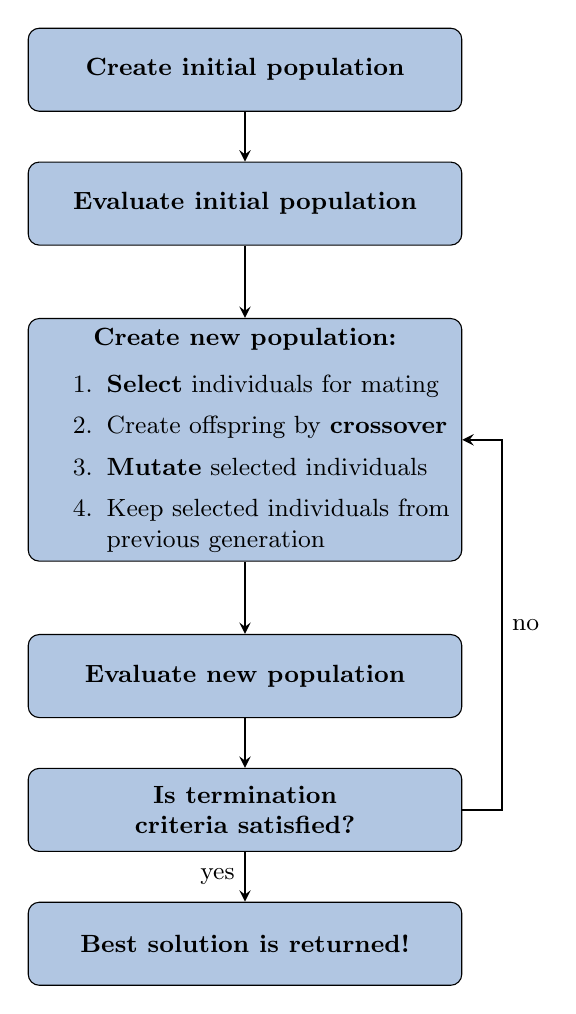
\begin{tikzpicture}[node distance=1.7cm]
                \tikzstyle{every node}=[font=\small]
                \node (1) [lbblock] {\textbf{Create initial population}};
                \node (2) [lbblock, below of=1] {\textbf{Evaluate initial population}};
                \node (3) [lbblock, below of=2, yshift = -1.3cm] {\textbf{Create new population:} \\ 
                \begin{enumerate} \item \textbf{Select} individuals for mating 
                                  \item Create offspring by \textbf{crossover} 
                                  \item \textbf{Mutate} selected individuals 
                                  \item Keep selected individuals from previous generation
                                 \end{enumerate}};
                \node (4) [lbblock, below of=3, yshift=-1.3cm] {\textbf{Evaluate new population}};
                \node (5) [lbblock, below of=4] {\textbf{Is termination \\ criteria satisfied?}};
                \node (6) [lbblock, below of=5] {\textbf{Best solution is returned!}};
                \draw [arrow] (1) -- (2);
                \draw [arrow] (2) -- (3);
                \draw [arrow] (3) -- (4);
                \draw [arrow] (4) -- (5);
                \draw [arrow] (5) -- node[anchor=east] {yes} (6);
                \draw [arrow] (5) -- ([shift={(0.5cm,0cm)}]5.east)-- node[anchor=west] {no} ([shift={(0.5cm,0cm)}]3.east)--(3);
        \end{tikzpicture}
        \caption{Process of finding optimal solutions for a problem with a 
        evolutionary algorithm \cite{renner_genetic_2003}. }
        \label{fig:genetic_alg}
\end{figure}

Genetic algorithms use mechanisms inspired by biological evolution, such as 
selection, crossover, and mutation. 
The three operators are simple and straightforward.
The crossover operator recombines good individuals to form a better 
individual. 
The mutation operator alters individuals to create better individuals
\cite{deb_multi-objective_2001}.  
The selection operator selects good individuals. 
The selection operator does not create new individuals in the population 
and only makes more copies of good individuals at the expense of not-so-good
individuals. 
The crossover and mutation operators perform the creation of new solutions.
Next, we provide more descriptions and common methods for each operator.

\subsubsection{Crossover/Mating Operator}
In most crossover operators, the operator randomly picks two individuals from 
the population. 
The operator exchanges some portion of each individuals' attributes with one 
another to create two new individuals \cite{deb_multi-objective_2001}. 
Crossover operator methods utilized in the proposed work include 
\textit{single-point crossover}, \textit{uniform crossover}, and 
\textit{blend crossover}. 
In the \textit{single-point crossover}, the operator randomly selects two 
individuals from the population and a site along the individual's definition. 
For example, if the individual is a list, the operator randomly chooses an element 
in the list as the cross-site. 
Then, the attributes on the cross site's right side are exchanged between the two 
individuals, creating two new offspring individuals. 
In a \textit{uniform crossover}, the user defines an independent exchange probability 
for each individual's attribute.
In \textit{blend crossover}, the operator creates two offspring (O) individuals based on 
a linear combination of two-parent (P) individuals using the following equations: 
\begin{align}
    O_1 &= P_1 - \alpha(P_1-P_2) \\
    O_2 &= P_2 + \alpha(P_1-P_2)
\intertext{where}
\alpha &= \mbox{Extent of the interval in which the new values can be drawn} \nonumber \\
 & \mbox{for each attribute on both side of the parents’ attributes (user-defined)} \nonumber 
\end{align}

The user defines a crossover probability ($p_c$) to preserve some good 
individuals selected during the selection operator stage.  
Therefore, the crossover operator only operates on $100p_c\%$ of the 
population; the rest proceed to the new population \cite{deb_multi-objective_2001}. 
The crossover operator covers the search aspect of the genetic algorithms, 
whereas the mutation operator keeps diversity in the population 
\cite{deb_multi-objective_2001}. 

\subsubsection{Mutation Operator}
The mutation operator alters one or more attributes of an individual within 
a population. 
Mutation operator methods utilized in the proposed work include 
\textit{polynomial bounded mutation}, in which each attribute in each individual 
is mutated based on a polynomial distribution. 
The user also defines each attribute's upper and lower bounds and the 
crowding degree of the mutation, $\eta$ (a big $\eta$ will produce a mutant 
resembling its parent, while a small $\eta$ will produce the opposite).
Mutation occurs in the genetic algorithm based on a user-defined mutation 
probability ($p_m$). 
A low $p_m$ prevents a primitive random search. 

\subsubsection{Selection Operator}
% this section needs improvement. 
The selection operator duplicates good individuals and eliminates bad individuals 
while keeping the population constant \cite{deb_multi-objective_2001}. 
It achieves this by identifying above-average individuals, eliminating bad 
individuals from the population, and replacing them with copies of good individuals.
Selection operator methods utilized in the proposed work include tournament 
selection, best selection, and \gls{NSGA-II} selection. 
In \textit{tournament selection}, a user-defined number of individuals play in a
tournament, and the best individual proceeds to the next population. 
The tournament repeats until all the population's spots are filled.
In \textit{best selection}, the operator selects a user-defined number of best 
individuals, and copies are made to keep the population size constant. 
For \textit{tournament} and \textit{best} selection operators, they maintain 
population size by adding copies of the best individuals. 
In \textit{NSGA-II selection}, the elitist operator selects the best individuals 
from the combination of parent and offspring populations \cite{deb_fast_2002}.
Only \textit{NSGA-II selection} can be used for multi-objective optimization. 

\subsection{Genetic Algorithm Hyperparameter Tuning}
Hyperparameters refer to parameters whose value controls 
the genetic algorithm's process, such as the population size. 
A well-performing genetic algorithm needs to balance the extent of exploration and 
exploitation; by finding a balance between the conservation of 
valuable individuals obtained until the current generation while exploring new 
individuals. 
With overexploitation of previously obtained individuals, the population loses 
diversity, resulting in premature convergence to a suboptimal solution. 
Alternatively, with over-exploration, the algorithm does not appropriately utilize 
the information obtained thus far, and the genetic algorithm's search procedure 
behaves like a random search process
\cite{deb_multi-objective_2001}. 

A quantitative balance between these two issues, exploitation and exploration, 
is challenging to achieve. 
Deb et al. \cite{deb_multi-objective_2001} and Goldberg et al. 
\cite{goldberg_toward_1993} quantified the relationship between exploitation 
and exploration. 
They found that for the one-max test problem, in which the objective seeks to 
maximize the number of 1s in a string, a genetic algorithm with any arbitrary 
hyperparameter setting does not work well even on a simple problem. 
Only genetic algorithms with a selection pressure (s) and crossover probability ($p_c$) 
falling inside the control map (Figure \ref{fig:controlmap}) will find the desired 
optimum.  
\begin{figure}[]
    \centering
    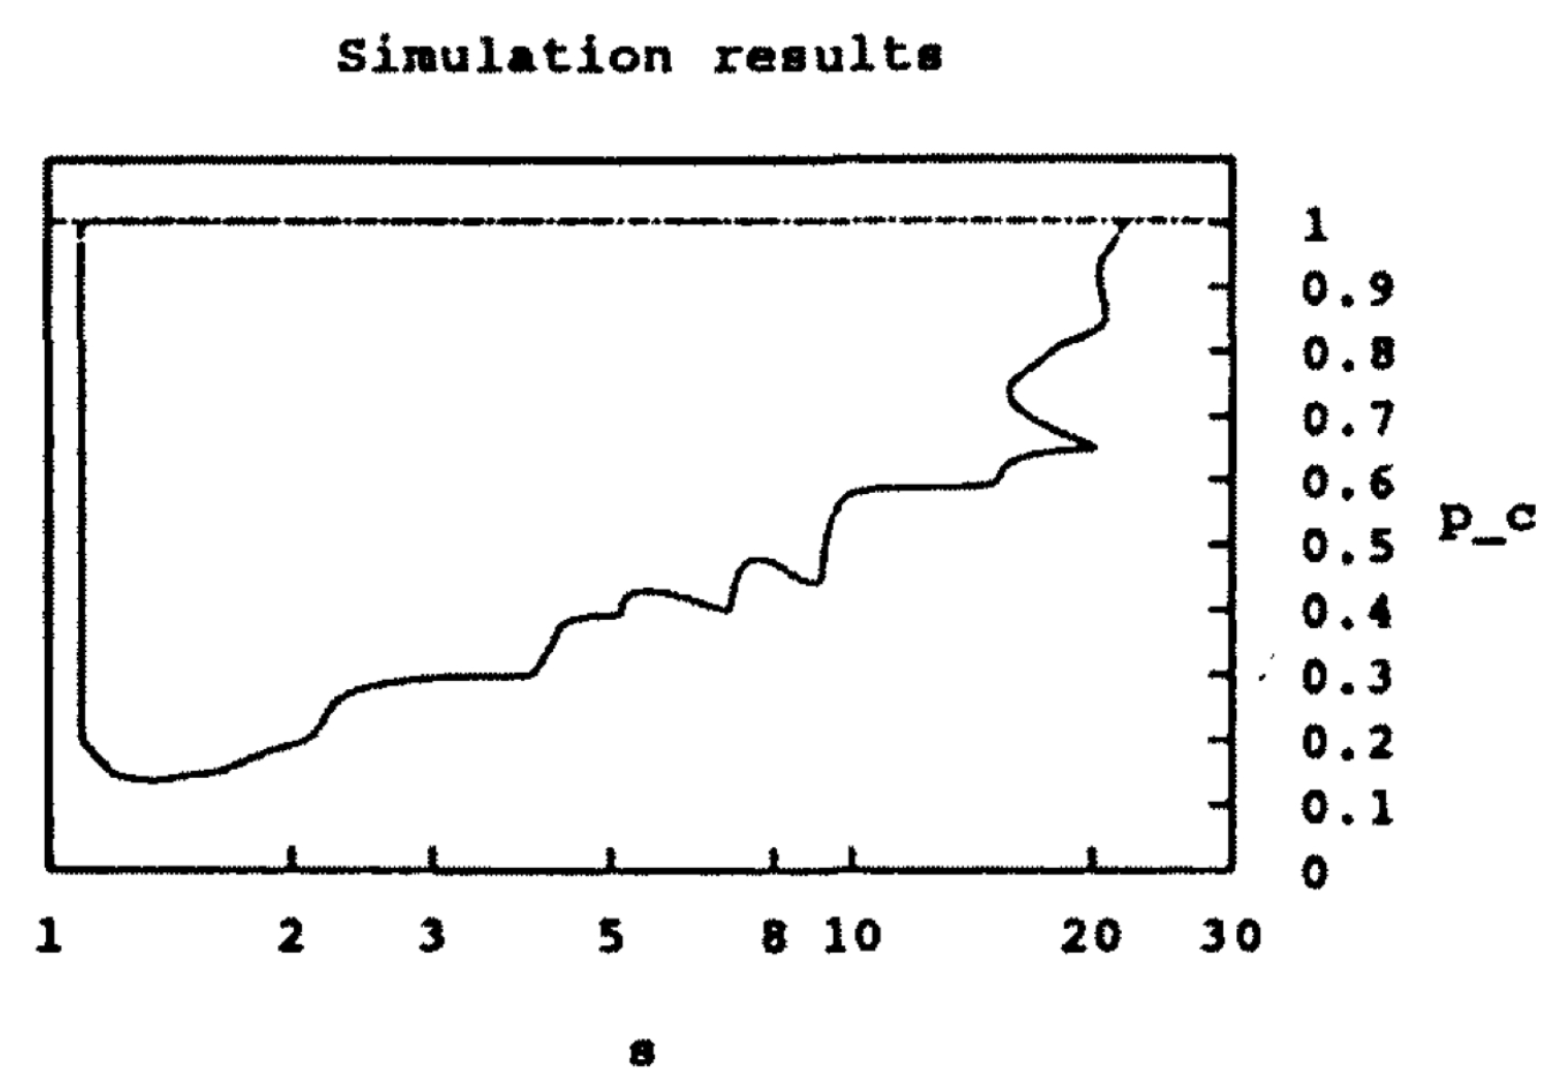
\includegraphics[width=0.6\linewidth]{controlmap.png} 
    \caption{Figure reproduced from \cite{goldberg_toward_1993,deb_multi-objective_2001}
    shows a control map region of selection pressure (s) and crossover probability ($p_c$)
    values in which the genetic algorithm will find the desired optimum for the 
    one-max problem.}
    \label{fig:controlmap}
\end{figure}
Another consideration is the population size. 
A function with considerable variability in objective function values demands 
a large population size to find a global optimum \cite{deb_multi-objective_2001}. 
Therefore, finding an optimized solution with genetic algorithms requires the user 
to conduct a hyperparameter search. 

Ng et al. \cite{ng_improving_2021} suggest that a coarse-to-fine sampling scheme 
is the best way to perform a systematic hyperparameter search.  
For a two-dimensional example of a coarse-to-fine sampling scheme, the user 
first does a coarse sample of the entire square, then a fine search on the 
coarse search's best-performing region. 
Ng et al. also suggest using random sampling over grid sampling because of the 
former's efficiency in high-dimensional spaces. 
Figure \ref{fig:random_vs_grid_sampling} illustrates how grid sampling gives 
even coverage in the original 2-d space but provides inefficient coverage in 
projections onto either the x1 or x2 subspace.  
In contrast, random sampling produces a less even distribution in the original 
space but a far more even distribution in the subspaces.
\begin{figure}[]
    \centering
    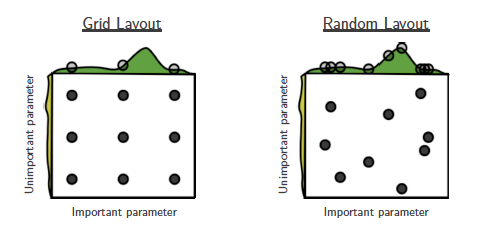
\includegraphics[width=0.8\linewidth]{random_vs_grid_sampling.png} 
    \caption{The impact of grid sampling vs random sampling on coverage of projections 
    into subspaces (reproduced from \cite{jordan_hyperparameter_2017}). 
    Random sampling has better coverage in the subspaces.}
    \label{fig:random_vs_grid_sampling}
\end{figure}

\section{Summary}
% this also needs improvement. 
This chapter provided a literature review of relevant past research 
efforts that give context to this dissertation. 
In summary, participation in the OECD-NEA FHR benchmarking exercise contributes 
to assessing the current neutron transport and thermal-hydraulics 
modeling and simulation capabilities for the \gls{AHTR} design.
Also, additive manufacturing of nuclear reactor components is a quickly 
developing field thanks to the aerospace and automotive industries, which led to 
breakthroughs in the additive manufacturing fabrication of metal components. 
The promise of cheaper and faster manufacturing of reactor components with 
additive manufacturing frees complex reactor geometries from previous 
manufacturing constraints and allows reactor designers to reexamine reactor 
design optimization.  
Stochastic optimization methods such as evolutionary algorithms have proven to 
work well for finding global optimums in multi-objective design problems such as 
nuclear reactor optimization and can be leveraged to explore the vast exploration 
design space enabled by additive manufacturing.

%\chapter{Fluoride-Salt-Cooled High-Temperature Reactor Benchmark}
\glsresetall
\label{chap:fhr-benchmark}
\gls{FHR} systems use \gls{TRISO} fuel and a low-pressure liquid fluoride-salt coolant.
\gls{FHR} technology combines \gls{FLiBe} coolant from \glspl{MSR} and 
\gls{TRISO} particles from \glspl{VHTR} to enable a reactor with 
low operating pressure, a large thermal margin, and accident-tolerant 
qualities.
Within the \gls{FHR} reactor class, \glspl{AHTR} have plate-based fuel in a hexagonal 
fuel assembly. 
In section \ref{sec:fhr}, I gave an \gls{FHR} concept overview, 
an \gls{AHTR} design description, a review of previous efforts 
towards modeling these designs, and how these efforts led to the \gls{FHR} benchmark
initiation. 

To address the \gls{AHTR} modeling challenges described in Chapter 
\ref{chap:lit-review}, such as multiple heterogeneity and material cross-section 
data, the \gls{OECD}-\gls{NEA} and \gls{Georgia Tech} initiated the \gls{FHR} 
benchmark for the \gls{AHTR} design in 2019 \cite{petrovic_benchmark_2021}. 
\gls{UIUC} participates in the \gls{FHR} benchmark with the OpenMC Monte Carlo code 
\cite{romano_openmc_2013} using the ENDF/B-VII.1 material cross section library 
\cite{chadwick_endf/b-vii.1_2011}.
The \gls{UIUC} team consists of myself and my advisors, Professor Kathryn Huff and Dr.
Madicken Munk. 

The three-phase \gls{FHR} benchmark begins with a single fuel assembly 
simulation without burnup and gradually extends to full core depletion. 
Table \ref{tab:phases} outlines the complete and incomplete benchmark phases as of 
August 2022.
\begin{table}[htbp]
    \centering
    \onehalfspacing
    \caption{\acrfull{OECD} \acrfull{NEA} \acrfull{FHR} benchmark Phases 
    \cite{petrovic_benchmark_2021}.}
	\label{tab:phases}
    \footnotesize
    \begin{tabular}{lclc}
    \hline 
    \textbf{Phases}& \textbf{Sub-phases} & \textbf{Description} & \textbf{Completed?} \\
    \hline
    \multirow{ 3}{5cm}{\textbf{Phase I: fuel assembly}} & I-A & 2D model, steady-state & \checkmark\\
    &I-B & 2D model depletion & \checkmark\\
    &I-C & 3D model depletion &\\
    \hline
    \multirow{2}{5cm}{\textbf{Phase II: 3D full core}}&II-A & Steady-state &\\
    &II-B & Depletion &\\
    \hline 
    \multirow{ 2}{5.5cm}{\textbf{Phase III: 3D full core with feedback \& multicycle analysis}}&III-A & Full core depletion with feedback &\\
    &III-B & Multicycle analysis &\\
    \hline
    \end{tabular}
\end{table}

In the subsequent sections, I will describe the benchmark's \gls{AHTR} design details
(Section \ref{sec:fhr-design} and Phase I specifications (Section \ref{sec:phase1}. 
Then, I will share our Phase I-A and I-B results generated with the OpenMC neutronics 
code \cite{romano_openmc_2013} (Section \ref{sec:fhr-phase1-results}) and the 
\gls{AHTR} temperature model's results (Section \ref{sec:fhr-bm-temp}).  
Appendix B lists all the data and analysis related to this chapter to enable the 
reproduction of all the simulations.

\section{FHR Benchmark \acrlong{AHTR} Design}
\label{sec:fhr-design}
Figure \ref{fig:reactor-schematic} shows the \acrfull{AHTR} schematic and a vertical 
cut of the reactor vessel. 
The \gls{AHTR} operates at 3400 MWt thermal power and 1400 MWe 
electric power \cite{varma_ahtr_2012}. 
\begin{figure}[htbp]
    \centering
    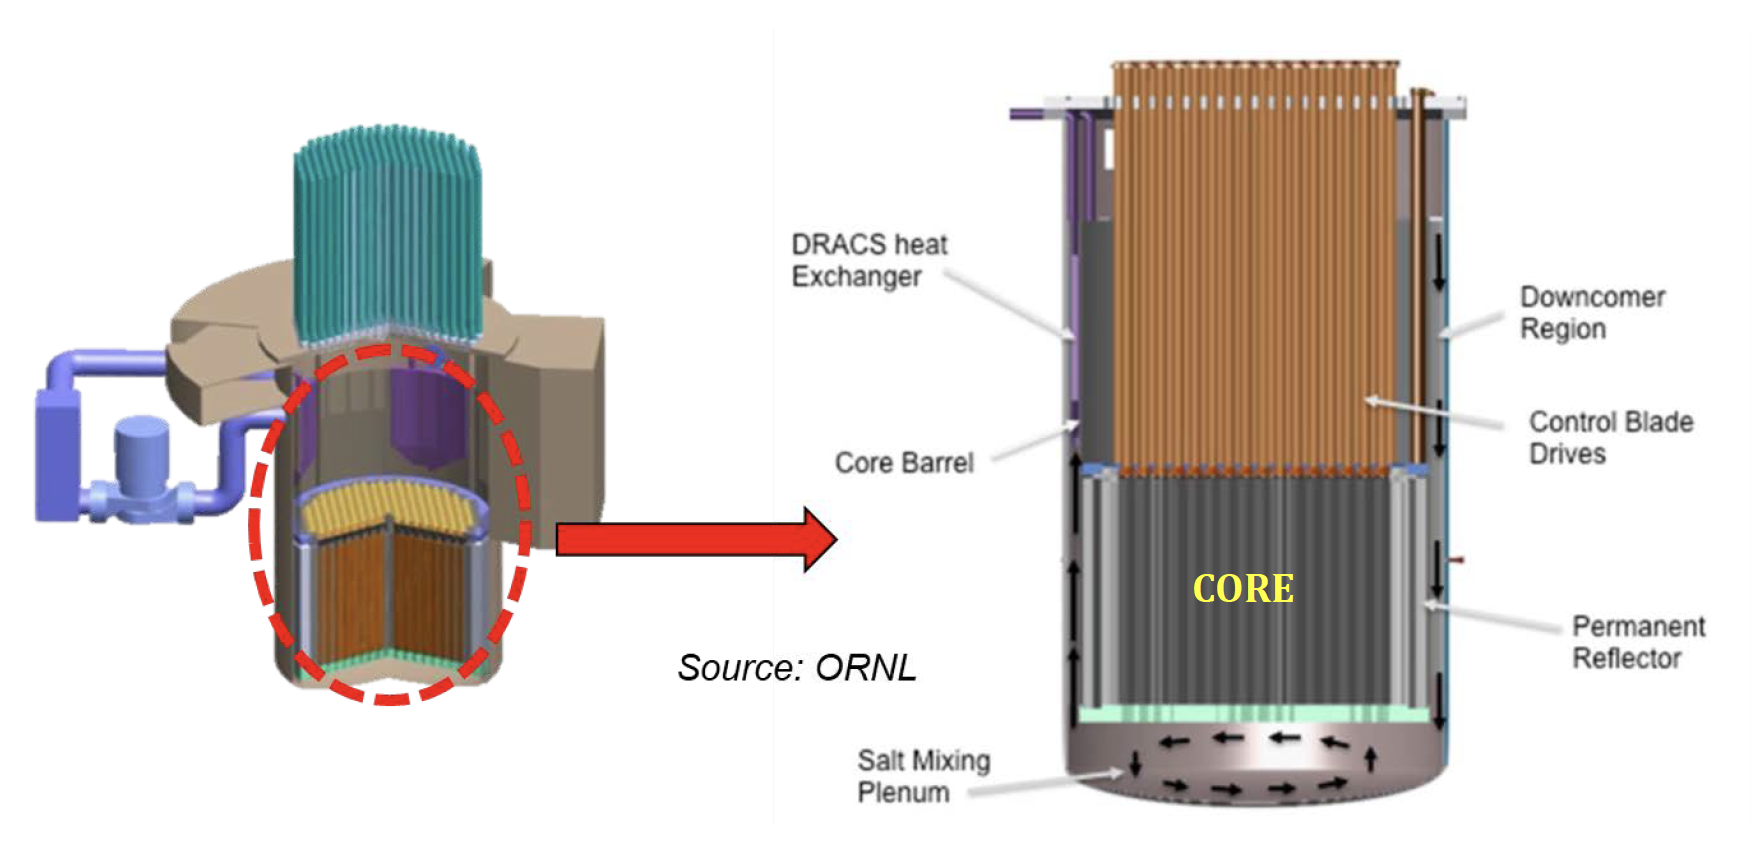
\includegraphics[width=\linewidth]{reactor-schematic.png} 
    \caption{\acrfull{AHTR} schematic (left) and vessel (right) reproduced from
    \cite{petrovic_benchmark_2021}.}
    \label{fig:reactor-schematic}
\end{figure}
The $10m$-diameter exterior reactor vessel contains an $8m$-diameter 
reactor core that contains 252 hexagonal fuel assemblies.

Each $6m$ high fuel assembly comprises a $5.5m$ active core region containing
\gls{TRISO} particles and $0.25m$ top and bottom non-fuelled reflector regions.
Figure \ref{fig:ahtr}, from Chapter \ref{chap:lit-review}, shows a single 
hexagonal fuel assembly geometry and the arrangement of all assemblies in the core.
All dimensions specified are at room temperature. 
The benchmark's phases I and II use room temperature dimensions, while Phase III 
will address dimensional changes brought about by temperature expansion. 
Figure \ref{fig:ahtr-fuel-assembly} shows a x-y plane view of the 
\gls{AHTR}'s hexagonal fuel assembly. 
\begin{figure}[htbp]
    \centering
    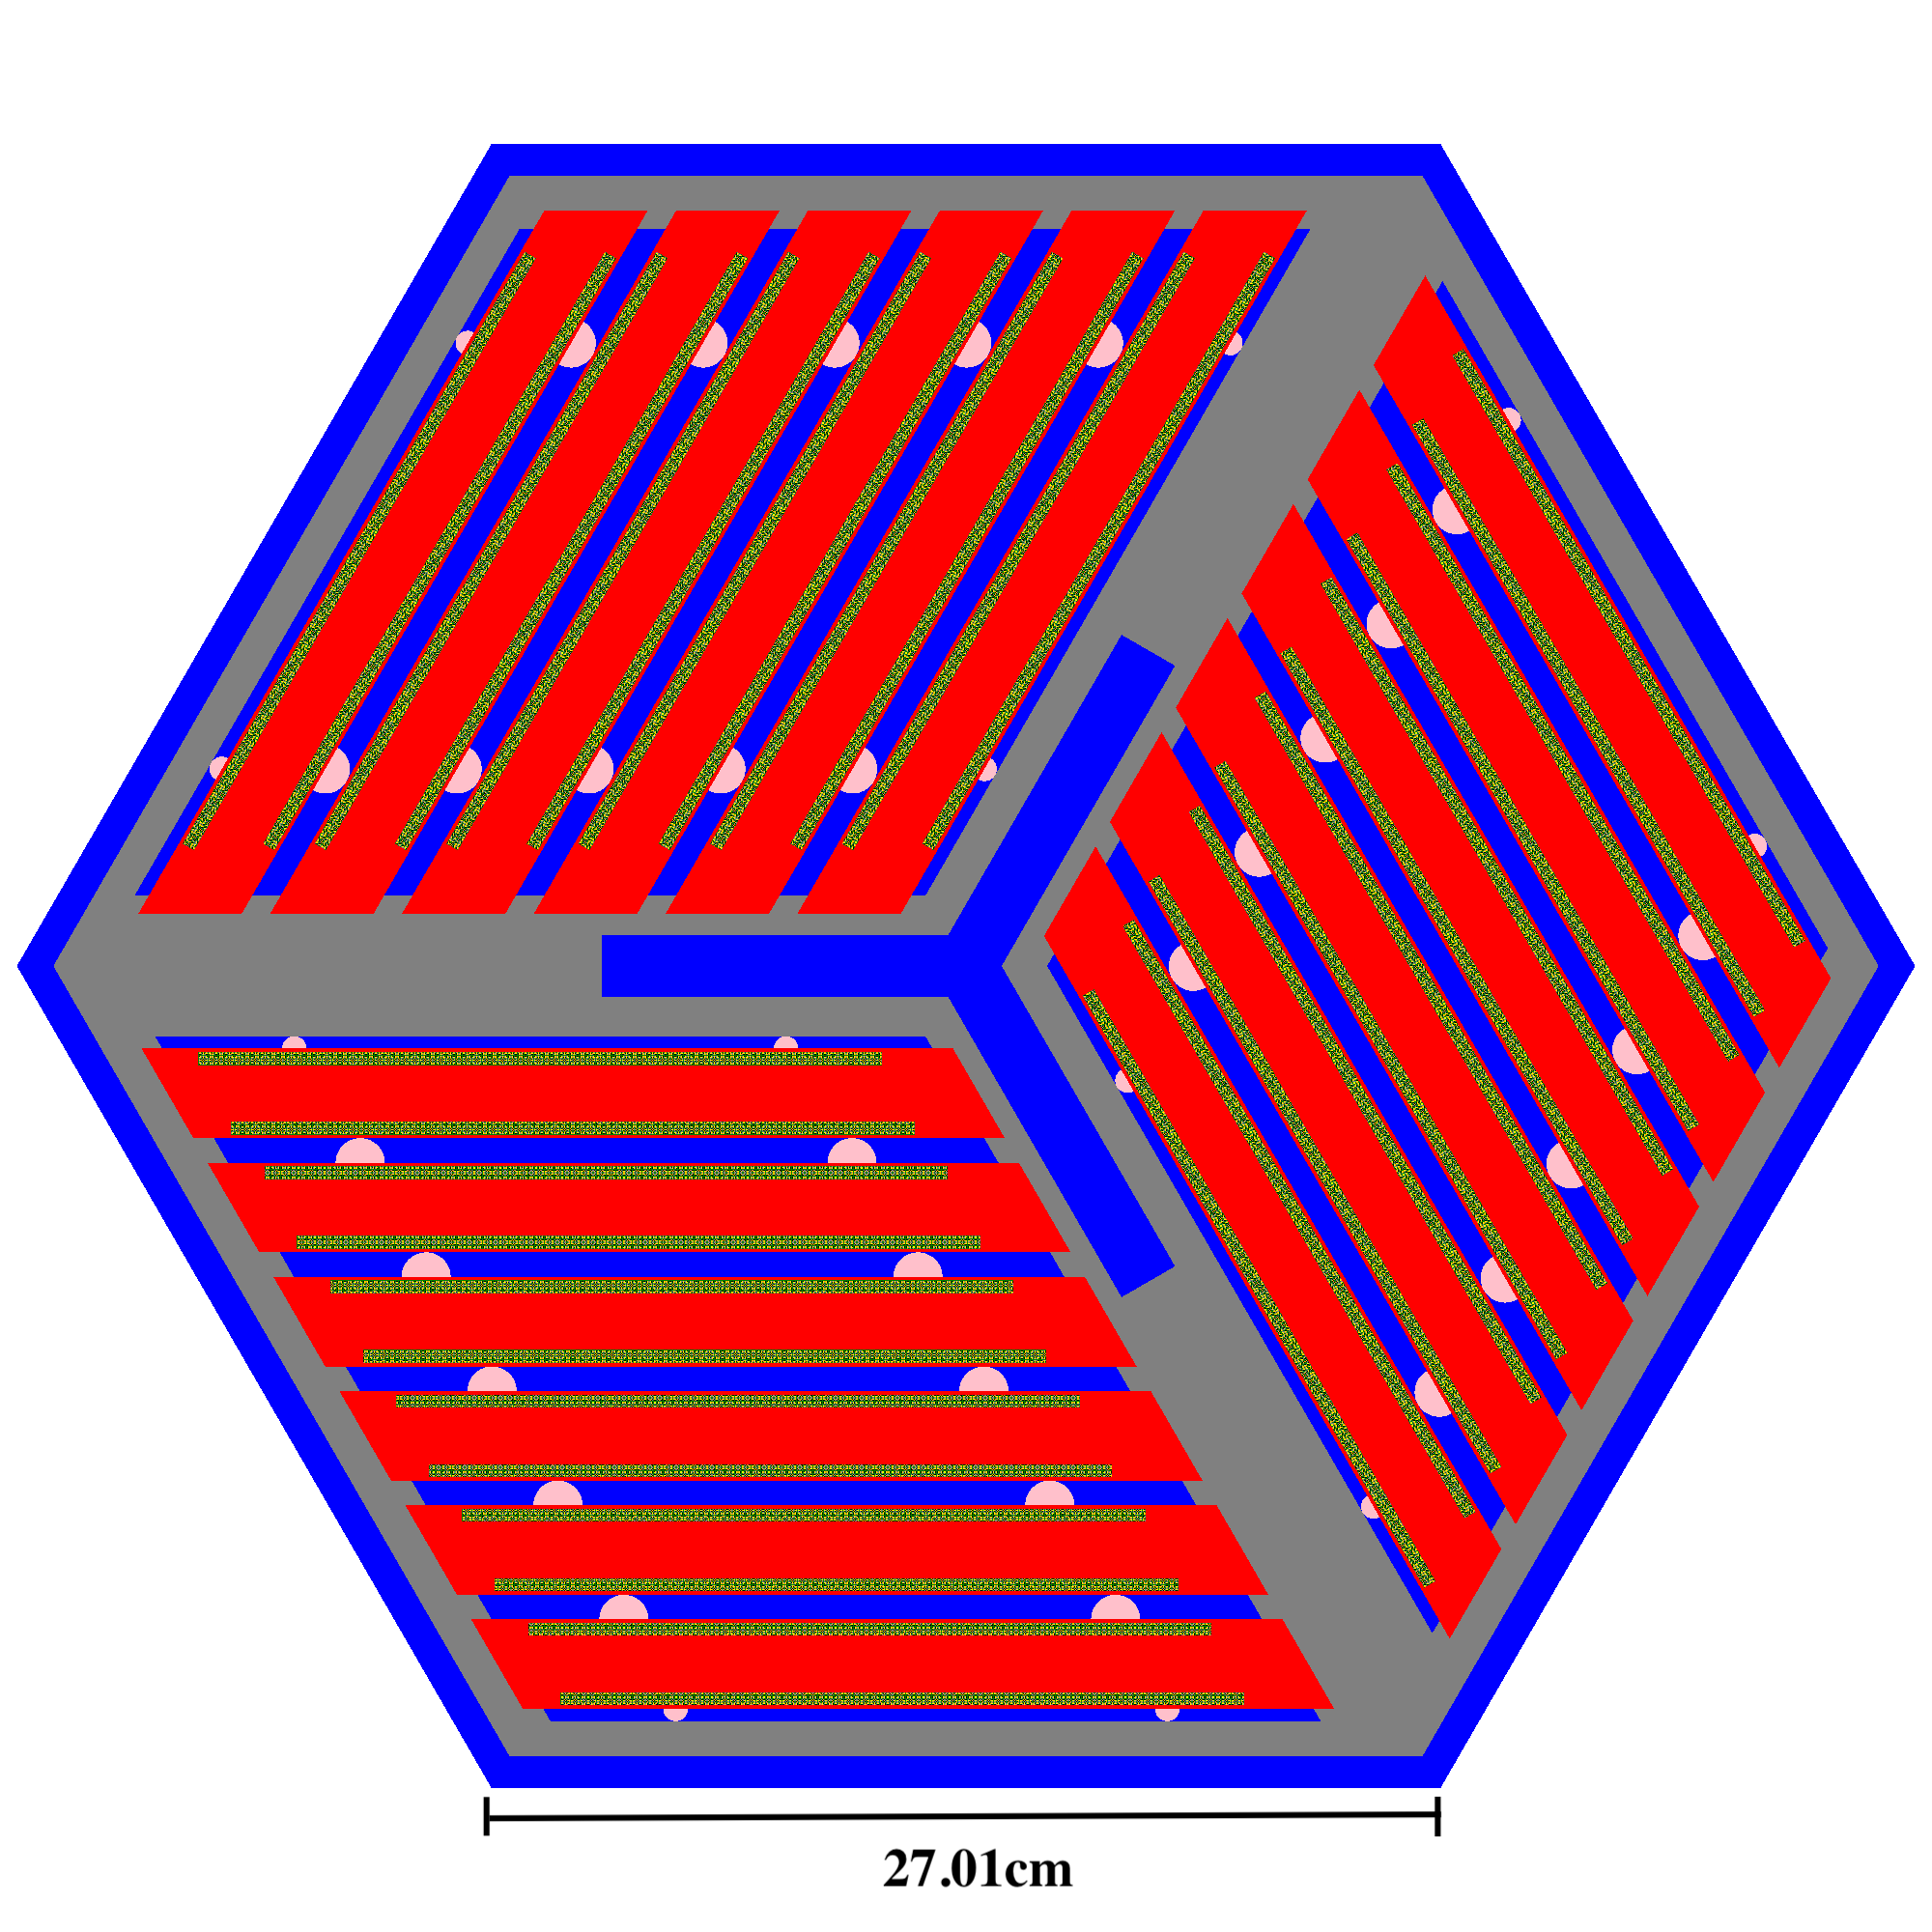
\includegraphics[width=0.9\linewidth]{ahtr-fuel-element.png} 
    \resizebox{0.4\textwidth}{!}{
        \fbox{\begin{tabular}{ll}
            \textcolor{fhrblue}{$\blacksquare$} & FLiBe \\
            \textcolor{fhrgrey}{$\blacksquare$} & Graphite (Fuel Structure)\\
            \textcolor{fhrred}{$\blacksquare$} & Graphite (Fuel Plank) \\
            \textcolor{fhrpink}{$\blacksquare$} & Graphite (Spacers) \\
            \textcolor{fhrgreen}{$\blacksquare$} & Graphite (Fuel Stripe) \\
            \textcolor{fhryellow}{$\blacksquare$} & TRISO particle \\
            \end{tabular}}}
            \hspace{0.5cm}
            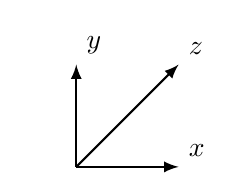
\begin{tikzpicture}
                \draw[ thick,-latex] (0,0) -- (1.3,0) node[anchor=south west] {$x$};
                \draw[ thick,-latex] (0,0) -- (0,1.3) node[anchor=south west] {$y$};
                \draw[ thick,-latex] (0,0) -- (1.3,1.3) node[anchor=south west] {$z$};
               \tkzText[above](-0.5,1){}
               \end{tikzpicture} 
    \caption{The \acrfull{FHR} benchmark's \acrfull{AHTR} fuel assembly with 18 fuel 
    planks (red) arranged in three diamond-shaped sectors, with a central Y-shaped and 
    external channel graphite structure (grey). 
    TRISO fuel (yellow) is arranged in a lattice structure within fuel stripes (green). 
    Spacers (pink) hold the graphite planks apart. 
    FliBe coolant flows through the assembly (blue). }
    \label{fig:ahtr-fuel-assembly}
\end{figure}
The hexagonal fuel assembly consists of eighteen fuel-containing graphite planks 
arranged in three diamond-shaped sectors, with an external channel wrapper and 
structural Y-shape, made of C-C composite with extra notches to hold the fuel 
planks in place. 
The diamond-shaped sections have $120^\circ{}$ rotational symmetry with each other 
\cite{varma_ahtr_2012,ramey_monte_2018,petrovic_benchmark_2021}. 
Semi-cylindrical graphite spacers attach to the fuel planks with a radius equalling to 
coolant channel thickness. 
\gls{FLiBe} coolant fills the gaps between the fuel planks and
assemblies (note: \gls{FLiBe} layer around the single assembly). 
The Y-shaped control rod slot at the center of the Y-shape structure contains 
\gls{FLiBe} coolant when the control blade is not in the slot (as seen in 
Figure \ref{fig:ahtr-fuel-assembly})
\cite{varma_ahtr_2012,ramey_monte_2018,petrovic_benchmark_2021}.
For a single fuel assembly, the internal $120^\circ{}$ rotational symmetry is 
represented by periodic boundary conditions, as seen in Figure \ref{fig:bc}. 
\begin{figure}[htbp]
    \centering
    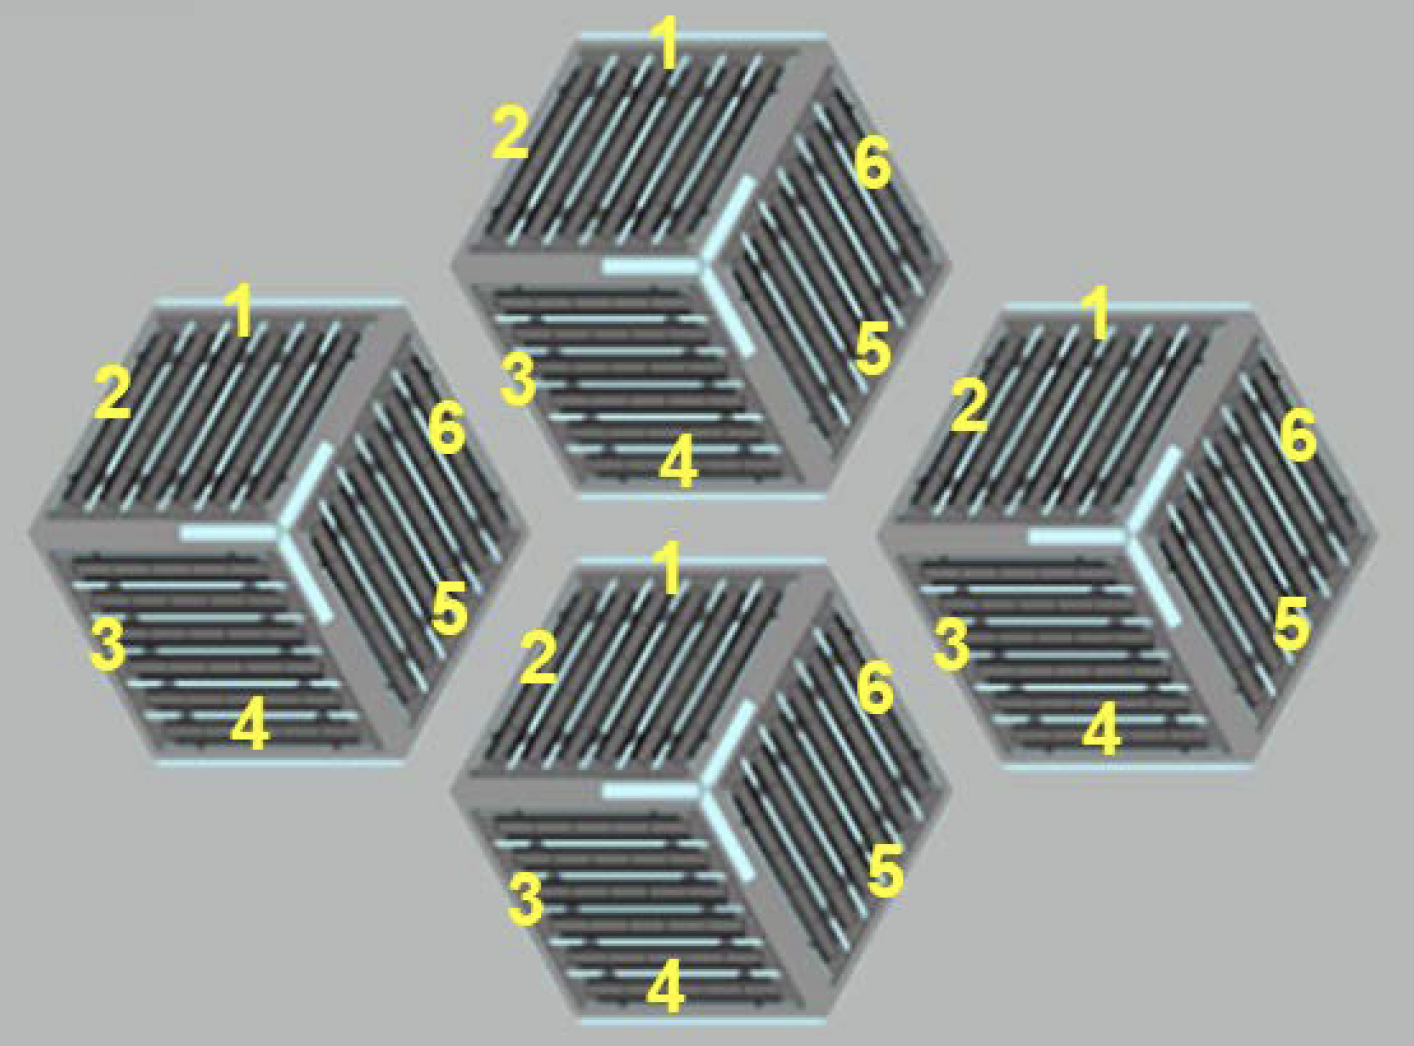
\includegraphics[width=0.72\linewidth]{bc.png} 
    \begin{tikzpicture}
        \draw[ thick,-latex] (0,7) -- (1.3,7) node[anchor=south west] {$x$};
        \draw[ thick,-latex] (0,7) -- (0,8.3) node[anchor=south west] {$y$};
        \draw[ thick,-latex] (0,7) -- (1.3,8.3) node[anchor=south west] {$z$};
       \tkzText[above](-0.5,0){}
       \end{tikzpicture} 
    \caption{Visualization of periodic boundary conditions for a single fuel 
    assembly in the \acrfull{AHTR}, reproduced from \cite{petrovic_benchmark_2021}.}
    \label{fig:bc}
\end{figure}

Figure \ref{fig:ahtr-fuel-plank} magnifies a single fuel plank. 
Fuel stripes line the upper and lower sides of each graphite fuel plank. 
\begin{figure}[htbp]
    \centering
    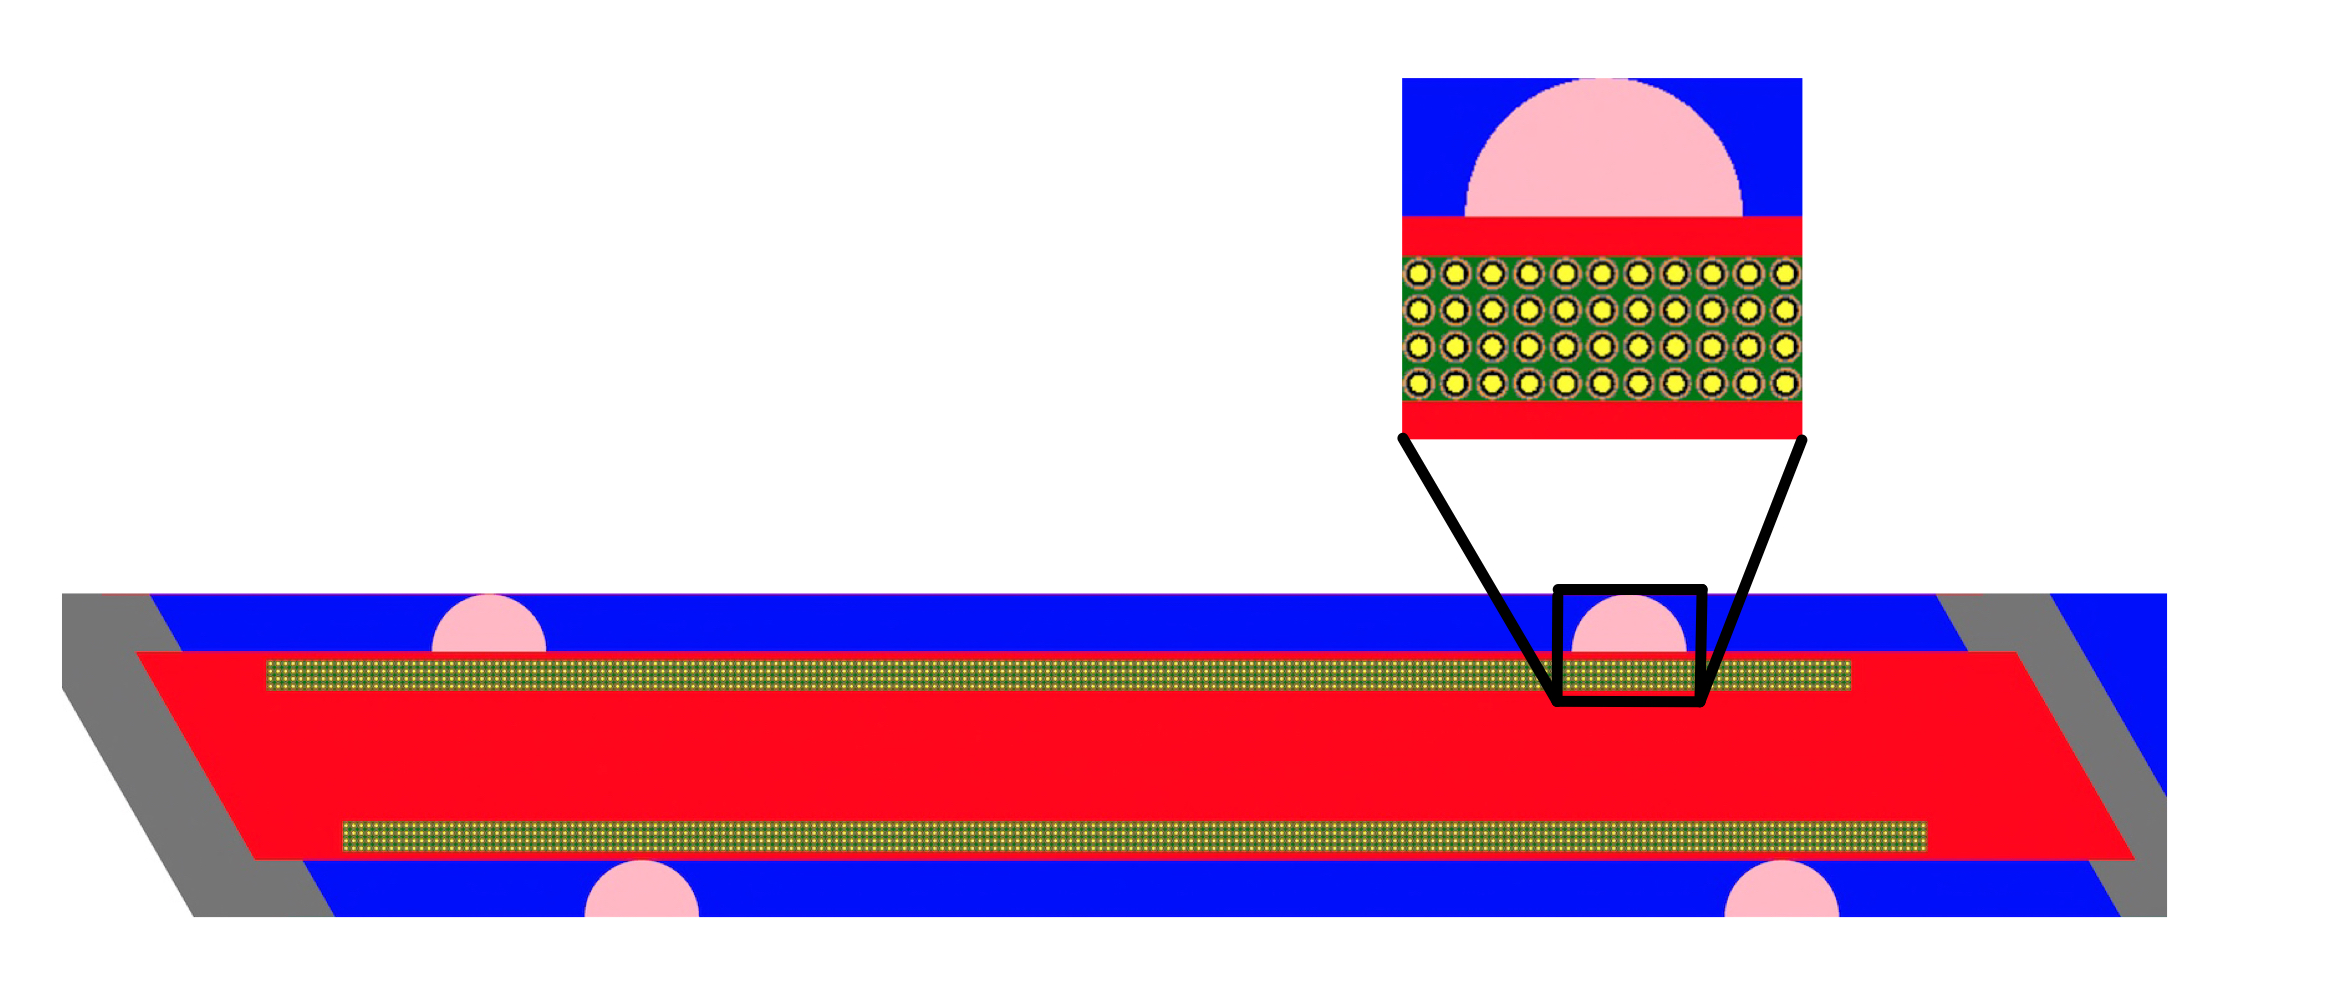
\includegraphics[width=\linewidth]{ahtr-fuel-plank.png} 
    \resizebox{0.4\textwidth}{!}{
        \fbox{\begin{tabular}{ll}
            \textcolor{fhrblue}{$\blacksquare$} & FLiBe \\
            \textcolor{fhrgrey}{$\blacksquare$} & Graphite (Fuel Structure)\\
            \textcolor{fhrred}{$\blacksquare$} & Graphite (Fuel Plank) \\
            \textcolor{fhrgreen}{$\blacksquare$} & Graphite (Fuel Stripe) \\
            \textcolor{fhryellow}{$\blacksquare$} & TRISO particle \\
            \textcolor{fhrpink}{$\blacksquare$} & Graphite (Spacer) \\
            \end{tabular}}}
            \hspace{0.5cm}
            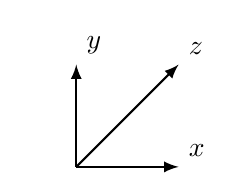
\begin{tikzpicture}
                \draw[ thick,-latex] (0,0) -- (1.3,0) node[anchor=south west] {$x$};
                \draw[ thick,-latex] (0,0) -- (0,1.3) node[anchor=south west] {$y$};
                \draw[ thick,-latex] (0,0) -- (1.3,1.3) node[anchor=south west] {$z$};
               \tkzText[above](-0.5,1){}
               \end{tikzpicture} 
    \caption{\acrfull{AHTR}'s fuel plank, with the magnification of 
    a spacer and segment of the fuel stripe with embedded \gls{TRISO} particles.}
    \label{fig:ahtr-fuel-plank}
\end{figure}
Each fuel stripe contains a graphite matrix filled with a cubic lattice of 
\gls{TRISO} particles with 40\% packing fraction. 
The lattice is 210 \gls{TRISO} particles wide in the x-direction, four particles 
deep in the y-direction, and 5936 particles tall in the z-direction. 
Figure \ref{fig:ahtr-triso} shows the \gls{TRISO} particle's cross section, 
consisting of five layers: oxycarbide fuel kernel, porous carbon buffer, 
inner pyrolytic carbon, silicon carbide layer, and the outer pyrolitic carbon. 
\begin{figure}[htbp]
    \centering
    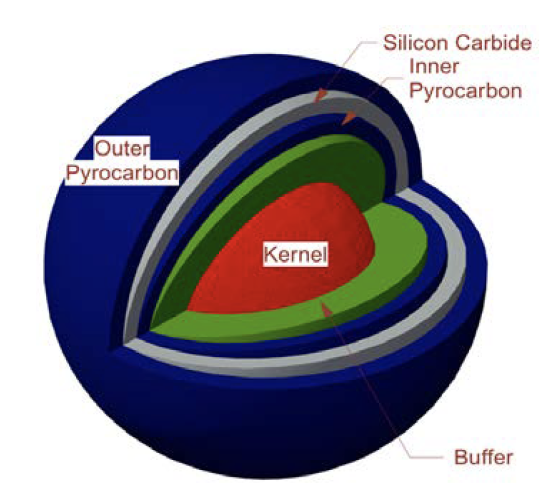
\includegraphics[width=0.6\linewidth]{ahtr-triso.png} 
    \caption{\acrlong{AHTR}'s TRISO particle schematic reproduced from 
    \cite{petrovic_benchmark_2021}.}
    \label{fig:ahtr-triso}
\end{figure}

The \gls{FHR} benchmark includes \gls{AHTR} configurations with burnable poisons 
and control rods to control reactivity. 
The burnable poisons consist of europium oxide ($Eu_2O_3$) and have a discrete
or integral (dispersed) option. 
Figure \ref{fig:discrete-poison} shows the discrete option with z-direction axially 
stacked small spherical $Eu_2O_3$ particles at five XY locations in each 
fuel plank. 
\begin{figure}[htbp]
    \centering
    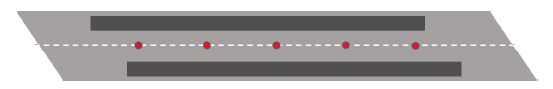
\includegraphics[width=0.82\linewidth]{discrete-poison.png}
    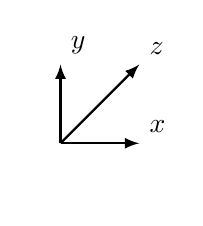
\begin{tikzpicture}
        \draw[ thick,-latex] (0,0) -- (1,0) node[anchor=south west] {$x$};
        \draw[ thick,-latex] (0,0) -- (0,1) node[anchor=south west] {$y$};
        \draw[ thick,-latex] (0,0) -- (1,1) node[anchor=south west] {$z$};
       \tkzText[above](-0.3,-0.7){}
       \end{tikzpicture} 
    \caption{x-y plane's placement of axial burnable poisons in the \acrlong{AHTR} 
    plank \cite{petrovic_benchmark_2021}. The burnable poisons are stacked in 
    the z-direction.}
    \label{fig:discrete-poison}
\end{figure}
The integral options consist of $Eu_2O_3$ homogenously mixed with the graphite 
fuel plank (including the graphite in fuel stripes matrix and plank ends 
indented to structural sides, but excluding the graphite in spacers and 
graphite in TRISO particles).
The \gls{MHC} control rod inserts into the Y-shaped control rod slot, displacing
the \gls{FLiBe} that occupies the slot 
(shown in Figure \ref{fig:ahtr-fuel-assembly}). 
Detailed \gls{AHTR} geometry and material information can be found in the 
\gls{FHR} benchmark's specifications \cite{petrovic_benchmark_2021}.

\section{FHR Benchmark Phase I Specifications}
\label{sec:phase1}
The \gls{FHR} benchmark Phase I consists of three subphases.
First, the steady-state 2D model (Phase I-A), next, the depletion of one 2D \gls{FHR} fuel 
assembly (Phase I-B), and finally depletion of one 3D \gls{FHR} fuel assembly 
(Phase I-C).
Benchmark organizers have only released Phase I-A and I-B's specifications. 
Thus Phase I-C's specifications will be omitted in this section.

The benchmark requires the following results for Phases I-A and I-B:
\begin{enumerate}[label=(\alph*)]
    \item $k_{eff}$ (effective multiplication factor)
    \item reactivity coefficients: $\beta_{eff}$ (effective delayed neutron fraction), 
    $\alpha_D$ (doppler coefficient), $\alpha_{T, FliBe}$ (\gls{FLiBe} temperature 
    coefficient), $\alpha_{M}$ (moderator temperature coefficient)
    \item tabulated fission source distribution by one-fifth fuel stripe
    \item $\bar{\phi_1}, \bar{\phi_2}, \bar{\phi_3}$ (neutron flux averaged over 
    the whole model tabulated in three coarse energy groups)
    \item $\phi_1(\vec{x},\vec{y}), \phi_2(\vec{x},\vec{y}), \phi_3(\vec{x},\vec{y})$ 
    (neutron flux distribution in three coarse energy groups) 
    \item fuel assembly averaged neutron spectrum
\end{enumerate}
Next, I report the equations used to calculate these required results.  

\subsubsection{Reactivity Coefficients (b)}
I assumed one energy group and six delayed groups for $\beta_{eff}$. 
Reactivity coefficient, $\alpha$, is the change in reactivity ($\rho$) of the 
material per degree change in the material's temperature (T). 
I calculated each reactivity coefficient and its corresponding uncertainty 
with these equations: 
\begin{align}
    \label{eq:reactivity-coefficient}
    \frac{\Delta \rho}{\Delta T} &= 
    \frac{\rho_{T_{high}}-\rho_{T_{low}}}{T_{high}-T_{low}} \ [\frac{pcm}{K}] \\
    \delta \frac{\Delta \rho}{\Delta T} &= 
    \frac{\sqrt{\delta (\rho_{T_{high}})^2+(\delta \rho_{T_{low}})^2}}{T_{high}-T_{low}} \ [\frac{pcm}{K}] 
\end{align}

\subsubsection{Fission Source Distribution / Fission Density (c)}
I calculated \gls{FD} with OpenMC's \texttt{fission} tally score (f) 
for each region divided by the average \texttt{fission} tally score of all the regions:
\begin{align}
    FD_i &=  \frac{f_i}{f_{ave}}\ [-]\\
    \intertext{where}
    f_i &= \mbox{fission reaction rate in a single region i [reactions/src]} \nonumber \\
    f_{ave} &= \mbox{average of all $f_i$ [reactions/src]} \nonumber
\end{align}
The uncertainty calculations for $FD_i$ and $f_{ave}$: 
\begin{align}
    \delta FD_i &= |FD_i| \sqrt{\left(\frac{\delta f_i}{f_i}\right)^2+\left(\frac{\delta f_{ave}}{f_{ave}}\right)^2} \\
    \delta f_{ave} &= \frac{1}{N}\sqrt{\sum_i^Nf_i^2} \\
    \intertext{where}
    N &= \mbox{No. of fission score values} \nonumber
\end{align}

\subsubsection{Neutron Flux (d, e, f)}
OpenMC's \texttt{flux} score is normalized per source particle simulated, resulting 
in [$\frac{neutrons\ cm}{src}$] units.
This is an unnatural unit for system analysis, and thus to better compare OpenMC
results with other software results in the benchmark, I converted flux to 
[$\frac{neutrons}{cm^2s}$] units using the following equations:  
\begin{align}
    \Phi_c &= \frac{N \cdot \Phi_o}{V} \\
    N &= \frac{P\cdot\nu}{Q\cdot k} \\
    \intertext{where}
    \Phi_c &= \mbox{converted flux [$\frac{neutrons}{cm^2s}$]} \nonumber \\ 
    \Phi_o &= \mbox{original flux [$\frac{neutrons\ cm}{src}$]} \nonumber \\
    N &= \mbox{normalization factor [$\frac{src}{s}$]} \nonumber \\
    V &= \mbox{volume of fuel assembly [$cm^3$]} \nonumber \\
    P &= \mbox{power [$\frac{J}{s}$]} \nonumber \\
    \nu &= \mbox{$\frac{\nu_f}{f}$ [$\frac{neutrons}{fission}$]} \nonumber \\
    Q &= \mbox{Energy produced per fission [$\frac{J}{fission}$]} \nonumber \\
    &= \mbox{$3.2044 \times 10^{-11}$ J per $U_{235}$ fission} \nonumber \\
    k &= \mbox{$k_{eff}$ [$\frac{neutrons}{src}$]} \nonumber 
\end{align}
The flux standard deviation is: 
\begin{align}
    \delta \Phi_c = \Phi_c \times
    \sqrt{(\frac{\delta \Phi_o}{\Phi_o})^2+ (\frac{\delta \nu_f}{\nu_f})^2 
    + (\frac{\delta k}{k})^2 + (\frac{\delta f}{f})^2}
\end{align}
I calculated reactor power based on the given reference specific power 
($P_{sp}$) of 200 $\frac{W}{gU}$: 
\begin{align}
    P &= P_{sp} \times V_F \times \rho_F \times \frac{wt\%_{U}}{100} \\
    \intertext{where}
    V_F &= \mbox{volume of fuel [$cm^3$]} \nonumber \\ 
    &= \frac{4}{3} \pi r_f^3 \times N_{total} \nonumber \\
    r_f &= \mbox{radius of fuel kernel within TRISO particle [cm]} \nonumber\\
    N_{total} &= \mbox{total no. of TRISO particles in fuel assembly} \nonumber \\ 
    &= 101 \times 210 \times 4 \times 2 \times 6 \times 3 \nonumber\\ 
    \rho_F &= \mbox{density of fuel [$g/cc$]} \nonumber \\
    wt\%_{U} &= \frac{at\%_{U235} \times m_{U235} + at\%_{U238} \times m_{U238}}{\sum (at\%_i \times m_i)} \times 100 \nonumber\\
    m &= \mbox{atomic mass} \nonumber
\end{align}

\subsection{Phase I-A Specifications}
For Phase I-A, the benchmark specifies that each participant must produce a 
steady-state 2D model of one fresh fuel assembly for nine cases
and report the required results listed in Section \ref{sec:phase1}.  
Table \ref{tab:phase1a-cases} describes each case. 
\begin{table}[htbp]
    \centering
    \onehalfspacing
    \caption{Description of the \acrlong{FHR} benchmark Phase I-A cases 
    \cite{petrovic_benchmark_2021}.}
    \footnotesize
	\label{tab:phase1a-cases}
    \begin{tabular}{p{0.05\textwidth}p{0.9\textwidth}}
    \hline 
    \textbf{Case} & \textbf{Description} \\
    \hline
    1A & Reference case. Hot full power (HFP), with temperatures of 1110K for 
    fuel kernel and 948K for coolant and all other materials (including TRISO 
    particle layers other than fuel kernel). Nominal (cold) dimensions, 
    9 wt\% enrichment, no \acrlong{BP}, \acrlong{CR} out.\\
    \hline
    2AH & \Gls{HZP} with uniform temperature of 948 K, 
    otherwise same as Case 1A. Comparison with Case 1A provides HZP-to-HFP power 
    defect.\\
    \hline 
    2AC & \Gls{CZP}. Same as Case 2AH, but with uniform temperature 
    of 773 K. Comparison with Case 2AH provides isothermal temperature coefficient.\\
    \hline
    3A & \Acrlong{CR} inserted, otherwise same as Case 1A. \\
    \hline
    4A & Discrete europia \acrlong{BP}, otherwise same as Case 1A.\\
    \hline
    4AR & Discrete europia \acrlong{BP} and \acrlong{CR} inserted, otherwise same as 
    Case 1A. \\
    \hline
    5A & Integral (dispersed) europia \acrlong{BP}, otherwise same as Case 1A. \\
    \hline
    6A & Increased \gls{HM} loading (4 to 8 layers of \gls{TRISO}) decreased C/HM 
    ratio (from about 400 to about 200) and decreased specific power to 100 W/gU, 
    otherwise same as Case 1A.\\
    \hline 
    7A & Fuel enrichment 19.75 wt\%, otherwise same as Case 1A.\\
    \hline 
    \end{tabular}
\end{table}

\subsection{Phase I-B Specifications}
For Phase I-B, the benchmark specifies that each participant must produce 
depletion results for three cases: 1B, 4B, and 7B. 
These are the same as cases 1A, 4A, and 7A (described in Table \ref{tab:phase1a-cases}), 
but with depletion steps added. 
The depletion steps are 0, 0.1, 0.5, 1, 2, 4, 6, 8, 10, 14, 18, 22, 26, 30, 40, 50, 
60, and 70 GWd/tU. 
Case 7B adds seven more depletion steps: 80, 90, 100, 120, 140, and 160 GWd/tU. 
The benchmark assumes that depletion occurs only in the fuel and burnable poisons 
and that the depletion performs under the critical spectrum assumption. 

\section{FHR Benchmark Phase I Results}
\label{sec:fhr-phase1-results}
The \texttt{arfc/fhr-benchmark} Github repository contains all the results submitted 
by \gls{UIUC} for the \gls{FHR} benchmark \cite{chee_arfcfhr-benchmark_2021}. 
The benchmark used a phased blind approach -- participants were asked to 
submit Phase I-A and I-B results without knowledge of other submissions. 
Petrovic et al. \cite{petrovic_preliminary_2021} describes the preliminary 
results of the benchmark across several institutions and concludes 
that the overall observed agreement is satisfactory. 
In the subsequent sections, I will share the results obtained by \gls{UIUC}. 

\subsection{Results: Phase I-A}
\label{sec:fhr-benchmark-results-ia}
In an \gls{ANS} Mathematics \& Computation (M$\&$C) 2021 conference, 
Petrovic et al. \cite{petrovic_preliminary_2021} 
compared \gls{FHR} benchmark participants' Phase I-A $k_{eff}$ results.  
We reported that the standard deviation between participants for each case 
was in the 231 to 514 pcm range, acceptable and notably close given a blind 
benchmark, assuring that \gls{UIUC}'s Phase I-A results are acceptable and 
in agreement with other benchmark participants. 

\subsubsection{Results: Effective Multiplication Factor (a)}
\label{sec:fhr-benchmark-keff}
Table \ref{tab:phase1a-results} reports Phase I-A $k_{eff}$ results. 
I ran the simulations on \gls{UIUC}'s BlueWaters supercomputer with 64 XE nodes, 
which each have 32 cores \cite{ncsa_about_2017}. 
To reduce the statistical uncertainty of $k_{eff}$ to $\sim$10pcm, I ran each 
simulation with 500 active cycles, 100 inactive cycles, and 200000 neutrons. 
Each simulation took \gls{WCT} ranging from 2 to 5 hours. 
\begin{table}[htbp]
    \centering
    \onehalfspacing
    \caption{\gls{UIUC}'s \acrlong{FHR} Benchmark Phase I-A results 
    \cite{chee_arfcfhr-benchmark_2021}.}
	\label{tab:phase1a-results}
    \footnotesize
    \begin{tabular}{cp{2.7cm}cccccc}
    \hline
    \textbf{Case} & \textbf{Summary} & \textbf{WCT [hr]} & \textbf{$k_{eff}$}* & 
    \textbf{$\beta_{eff}$}** & 
    \textbf{Fuel} $\frac{\Delta \rho}{\Delta T}$ & 
    \textbf{FliBe} $\frac{\Delta \rho}{\Delta T}$ & 
    \textbf{Graphite} $\frac{\Delta \rho}{\Delta T}$\\
    \hline 
    1A & Reference &2.82&1.39389 & 0.006534 & -2.24$\pm$0.15 & -0.15$\pm$0.15 & -0.68$\pm$0.15\\
    2AH & \gls{HZP} &2.82&1.40395 & 0.006534 & -3.14$\pm$0.15 & -0.20$\pm$0.14 & -0.85$\pm$0.14\\
    2AC & \gls{CZP} &2.75&1.41891 & 0.006534 & -3.36$\pm$0.14 & -0.11$\pm$0.14 & 0.07$\pm$0.14\\
    3A & CR &2.49&1.03147 & 0.006534 & -4.03$\pm$0.28 & -0.83$\pm$0.27 & -3.18$\pm$0.29\\
    4A & Discrete BP &5.08&1.09766 & 0.006542 & -4.06$\pm$0.24 & -1.55$\pm$0.23 & -6.51$\pm$0.24\\
    4AR & Discrete BP + CR &4.59&0.84158 & 0.006553 & -5.60$\pm$0.49 & -1.78$\pm$0.46 & -10.44$\pm$0.47\\
    5A & Dispersed BP &2.33&0.79837 & 0.006556 & -5.09$\pm$0.40 & -4.87$\pm$0.40 & -22.99$\pm$0.38\\
    6A & Increased \gls{HM} &3.52&1.26294 & 0.006556 & -4.46$\pm$0.19 & 0.16$\pm$0.20 & -0.39$\pm$0.20\\
    7A & 19.75\% Enriched &2.21&1.50526 & 0.006530 & -2.49$\pm$0.13 & -0.12$\pm$0.12 & -0.62$\pm$0.12\\
    \hline
    \multicolumn{5}{l}{BP: burnable poison, CR: control rod} \\
    \multicolumn{5}{l}{* All $k_{eff}$ values have an uncertainty of 0.00010.} \\
    \multicolumn{5}{l}{** All $\beta_{eff}$ values have an uncertainty of 0.000001.}
    \end{tabular}
\end{table}

Cases 2AH and 2AC are at zero power, meaning that the fuel assembly is exactly 
critical but not producing any energy. 
For both cases, $k_{eff}$ is higher than the reference Case 1A, which I attribute to 
lower fuel temperatures. 
At lower fuel temperatures, less doppler broadening occurs, resulting in less neutron 
capture, thus, increasing $k_{eff}$. 
As expected, $k_{eff}$ is lower for Cases 3A, 4AR, and 5A than reference case 
1A since these cases introduce burnable poisons and control rods to the fuel 
assembly. 
Also, as expected, $k_{eff}$ is higher for Case 7A than reference Case 1A since 
it has a higher enrichment. 
However, Case 6A deviated from expectations with a lower $k_{eff}$ despite an increase 
in \acrlong{HM} loading. 
This behavior is due to reduced moderation and worsened fuel utilization brought about 
by self-shielding, demonstrating that increased fuel packing fraction does not 
always correspond with an increased $k_{eff}$. 

\subsubsection{Results: Reactivity Coefficients (b)}
Table \ref{tab:phase1a-results} reports Phase I-A reactivity coefficients results. 
$\beta_{eff}$ increased by 10-20 [pcm] for Cases 4A, 4AR, 5A, and 6A compared to
reference Case 1A due to the introduction of control rods and poisons that 
shift the average neutron velocity to higher values, resulting in decreased
thermal fission and increased fast fission \cite{torabi_neutronic_2018}.
In Table \ref{tab:phase1a-results}, most temperature coefficients are negative, 
exemplifying the \gls{AHTR}'s passive safety behavior. 
Negative reactivity feedback results in a self-regulating reactor; if the reactor 
power rises, resulting in a temperature increase, the negative reactivity
reduces power. 

\subsubsection{Results: Fission Source Distribution (c)}
Figure \ref{fig:phase1a-c} shows Cases 1A and 3A's fission source distribution 
discretized by one-fifth fuel stripe. 
\begin{figure}[htbp]
    \centering
    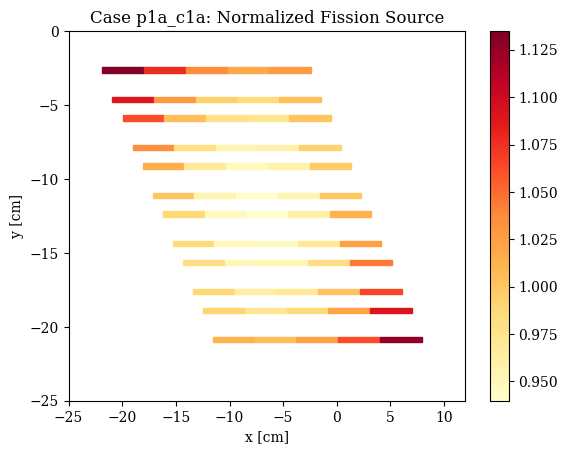
\includegraphics[width=0.49\linewidth]{p1a_c1a_c.png} 
    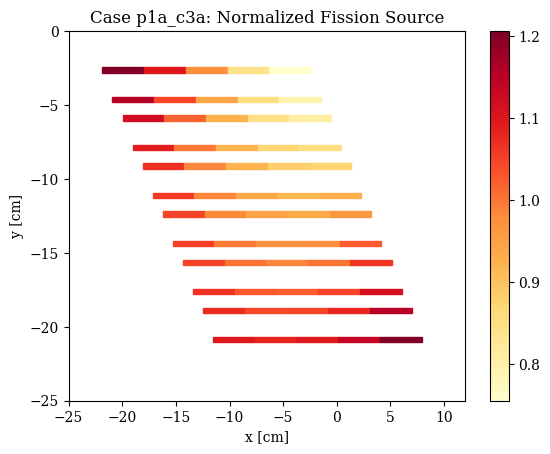
\includegraphics[width=0.49\linewidth]{p1a_c3a_c.png} 
    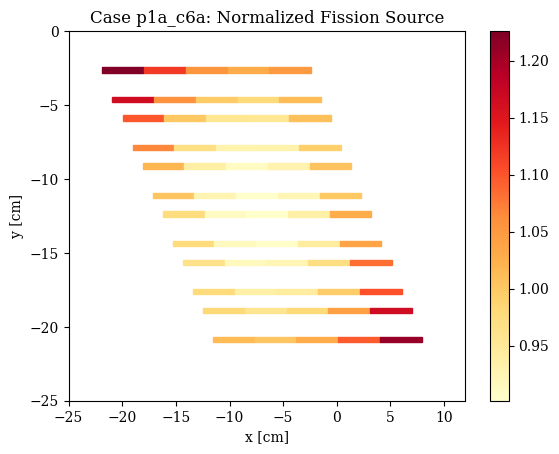
\includegraphics[width=0.49\linewidth]{p1a_c6a_c.png} 
    \caption{\gls{UIUC} \gls{FHR} benchmark results: normalized Fission Source 
    Distribution [-] per one-fifth fuel stripe for \acrlong{FHR} Benchmark's Phase I-A 
    Case 1A (top left), Case 3A (top right), and Case 6A (bottom).}
    \label{fig:phase1a-c}
\end{figure}
Case 4AR has a similar fission source distribution to Case 3A since both 
cases have control rod insertion. 
Case 7A has a similar fission source distribution to case 6A since both have 
higher heavy metal loading. 
All other cases have similar fission source distributions to Case 1A. 

For Case 1A, intuitively, one might assume that the highest fission source would 
occur in the center of the diamond fuel segment; however, the opposite is true. 
Power peaking occurs on exterior stripes and is minimum on the interior stripes.
Gentry et al. \cite{gentry_development_2016} reported similar power peaking 
phenomena towards the lattice cell's exterior closest to the Y-shaped carbon 
support structure.  
This fission source distribution is caused by diminished resonance escape 
probability in the interior due to the higher relative fuel-to-carbon volume 
ratio. 

For Case 3A with an inserted control rod, the fission source is lower in 
the one-fifth stripes closer to the control rod.  
Case 6A demonstrates a further diminished fission source in the interior 
stripes due to the higher fuel-to-carbon ratio.
This is seen in Figure \ref{fig:phase1a-c}, in which case 1A and 6A have similar 
fission distribution trends, but case 6A has a bigger fission source value range. 

\subsubsection{Results: Average Neutron Flux (d)}
Figure \ref{fig:phase1a-d} shows the average neutron flux in the fuel assembly in 
three coarse energy groups. 
\begin{figure}[htbp]
    \centering
    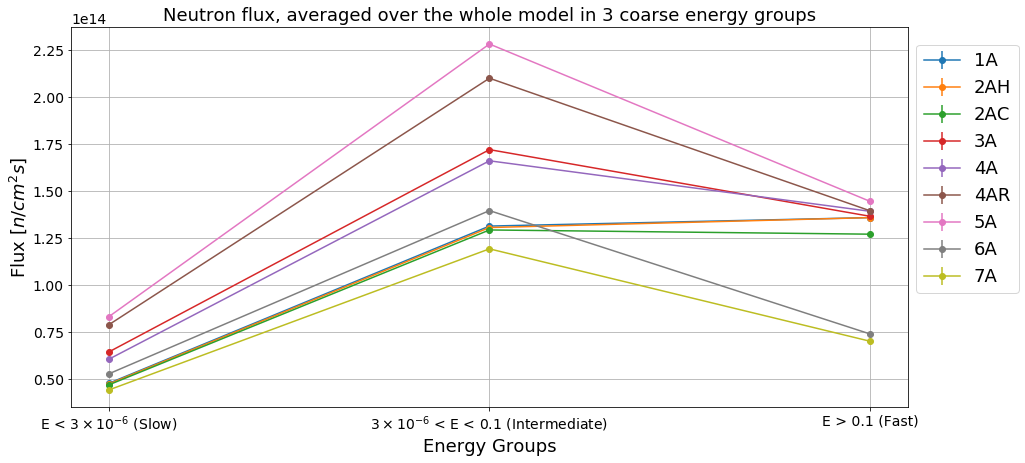
\includegraphics[width=\linewidth]{phase1a-d-flux.png} 
    \caption{\gls{UIUC} \gls{FHR} benchmark results: neutron flux, 
    averaged over the whole model, tabulated in three coarse energy groups for 
    each Phase I-A case. Neutron flux uncertainty is on the order of 1e10.}
    \label{fig:phase1a-d}
\end{figure}
Most cases have the most flux in the intermediate group, followed by 
the thermal group, and the least flux in the fast group.   

\subsubsection{Results: Neutron Flux Distribution (e)}
Figure \ref{fig:phase1a-e} shows the neutron flux distribution in a 100 $\times$ 
100 mesh for Cases 1A, 3A, and 6A for three coarse energy groups. 
\begin{figure}[htbp]
    \centering
    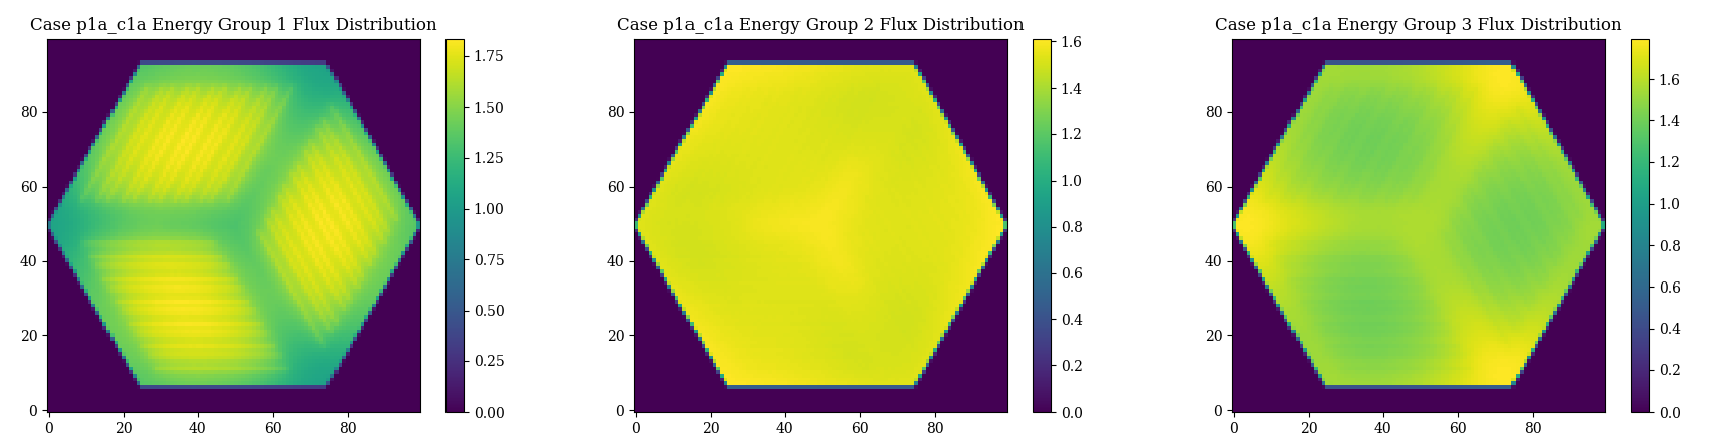
\includegraphics[width=\linewidth]{phase1a-e-c1a.png} 
    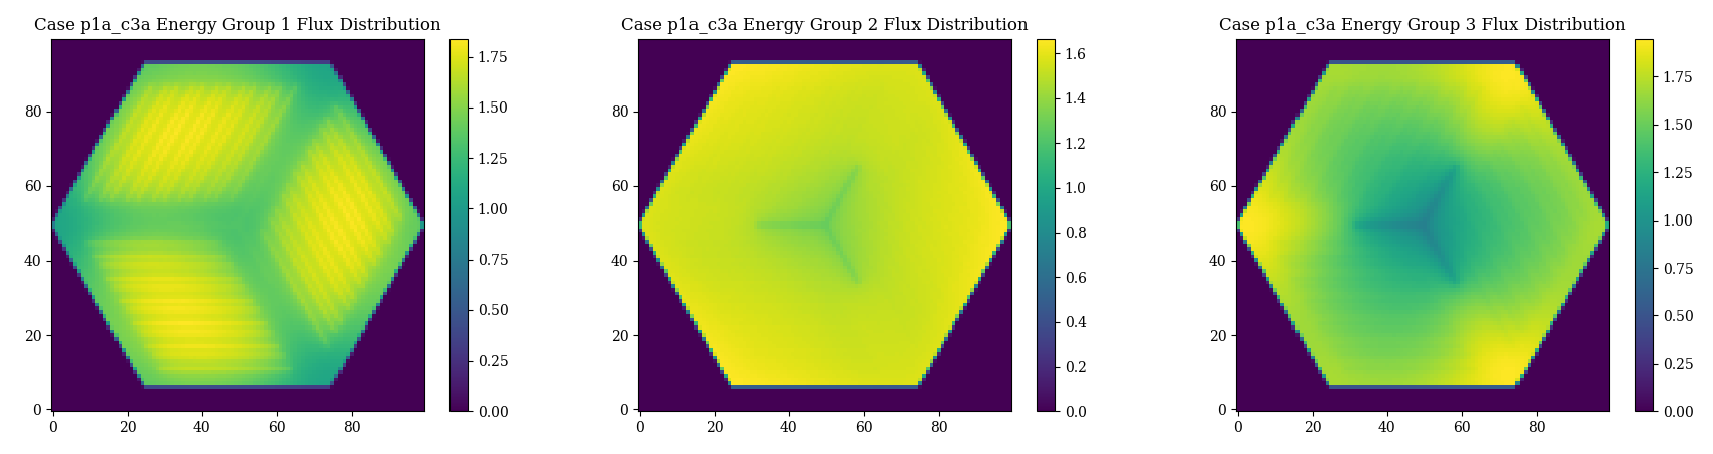
\includegraphics[width=\linewidth]{phase1a-e-c3a.png} 
    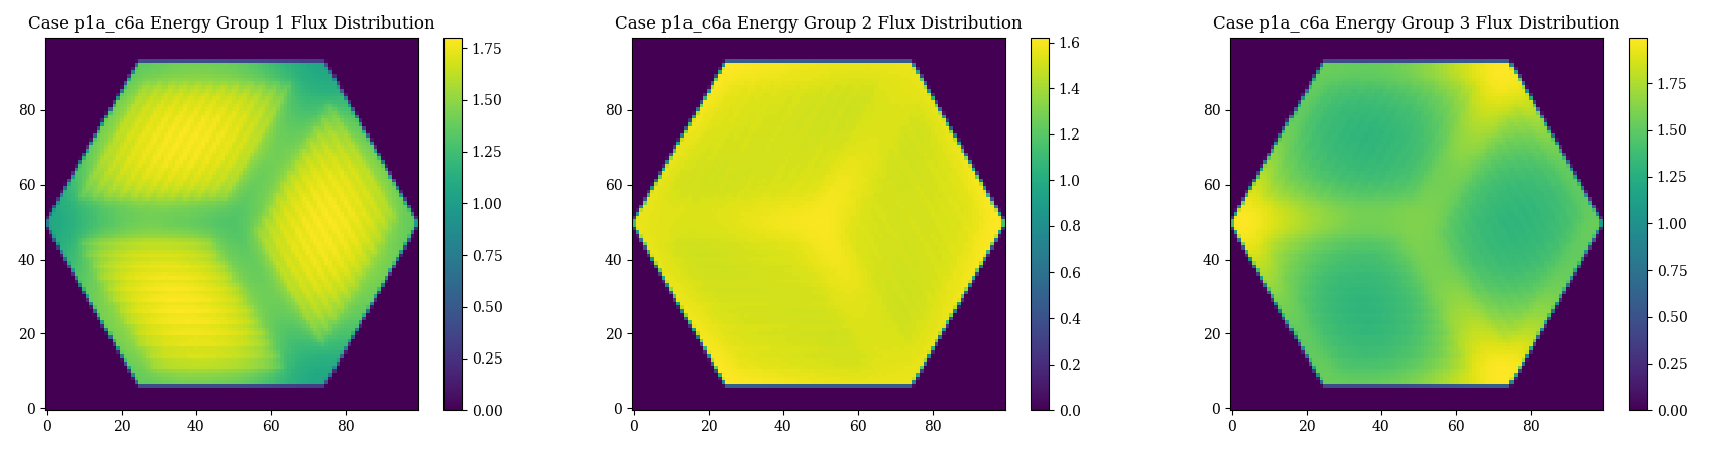
\includegraphics[width=\linewidth]{phase1a-e-c6a.png} 
    \caption{\gls{UIUC} \gls{FHR} benchmark flux results: neutron flux 
    distribution in 100 $\times$ 100 mesh for three coarse energy groups: Case 
    1A (above), Case 3A (middle), Case 6A (below). Energy group 1: $E > 0.1$ MeV, 
    Energy group 2: $3 \times 10^{-6} < E < 0.1$ MeV, Energy group 3: $E < 3 \times 10^{-6}$ MeV. }
    \label{fig:phase1a-e}
\end{figure}
% TODO: add axes labels and bigger... 
For all three cases, fast-flux (energy group 1) peaks in the diamond-shaped sectors containing 
the fuel stripes, whereas thermal flux (energy group 3) peaks outside the diamond-shaped 
sectors. 
This can be attributed to fission occurring at thermal energies in the fuel stripe area. 
For Case 3A, the thermal and intermediate neutron flux is depressed in the fuel 
assembly's control rod region.  
An increased heavy metal loading in Case 6A results in a more pronounced 
fast-flux peaking and thermal flux dip in the fuel stripe area. 

\subsubsection{Results: Neutron Spectrum (f)}
Figure \ref{fig:phase1a-f} shows the neutron spectrum for Cases 1A and 6A. 
\begin{figure}[htbp]
    \centering
    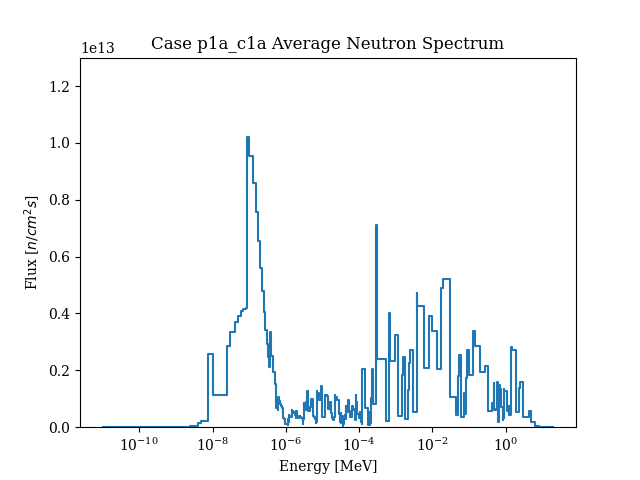
\includegraphics[width=0.49\linewidth]{p1a_c1a_f.png} 
    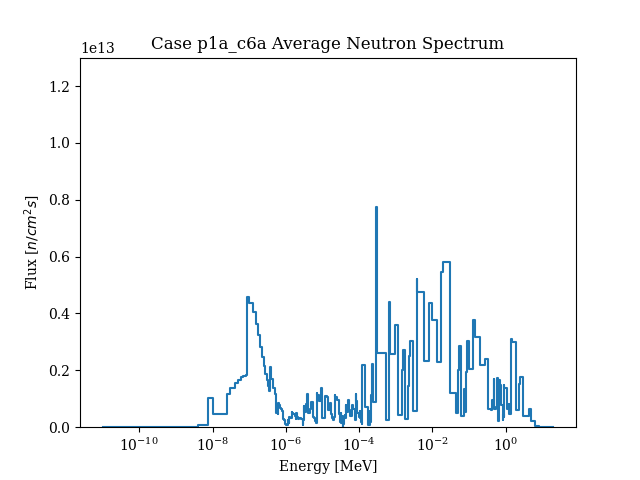
\includegraphics[width=0.49\linewidth]{p1a_c6a_f.png} 
    \caption{\gls{UIUC} \gls{FHR} benchmark results: neutron spectrum for 
    Phase I-A Case 1A (left) and Case 6A (right).}
    \label{fig:phase1a-f}
\end{figure}
% todo: increase label sizes... 
Case 7A has a similar neutron spectrum to Case 6A since both cases have 
higher fuel content. 
All other cases have a similar neutron spectrum to Case 1A.
The neutron spectra in Cases 6A and 7A are faster due to more heavy metal 
loading and higher enrichment, respectively.  

\subsection{Results: Phase I-B}
\label{sec:fhr-benchmark-results-ib}
Figure \ref{fig:phase1b_keff} shows the $k_{eff}$ evolution during depletion 
for Cases 1B, 4B, and 7B.
\begin{figure}[htbp]
    \centering
    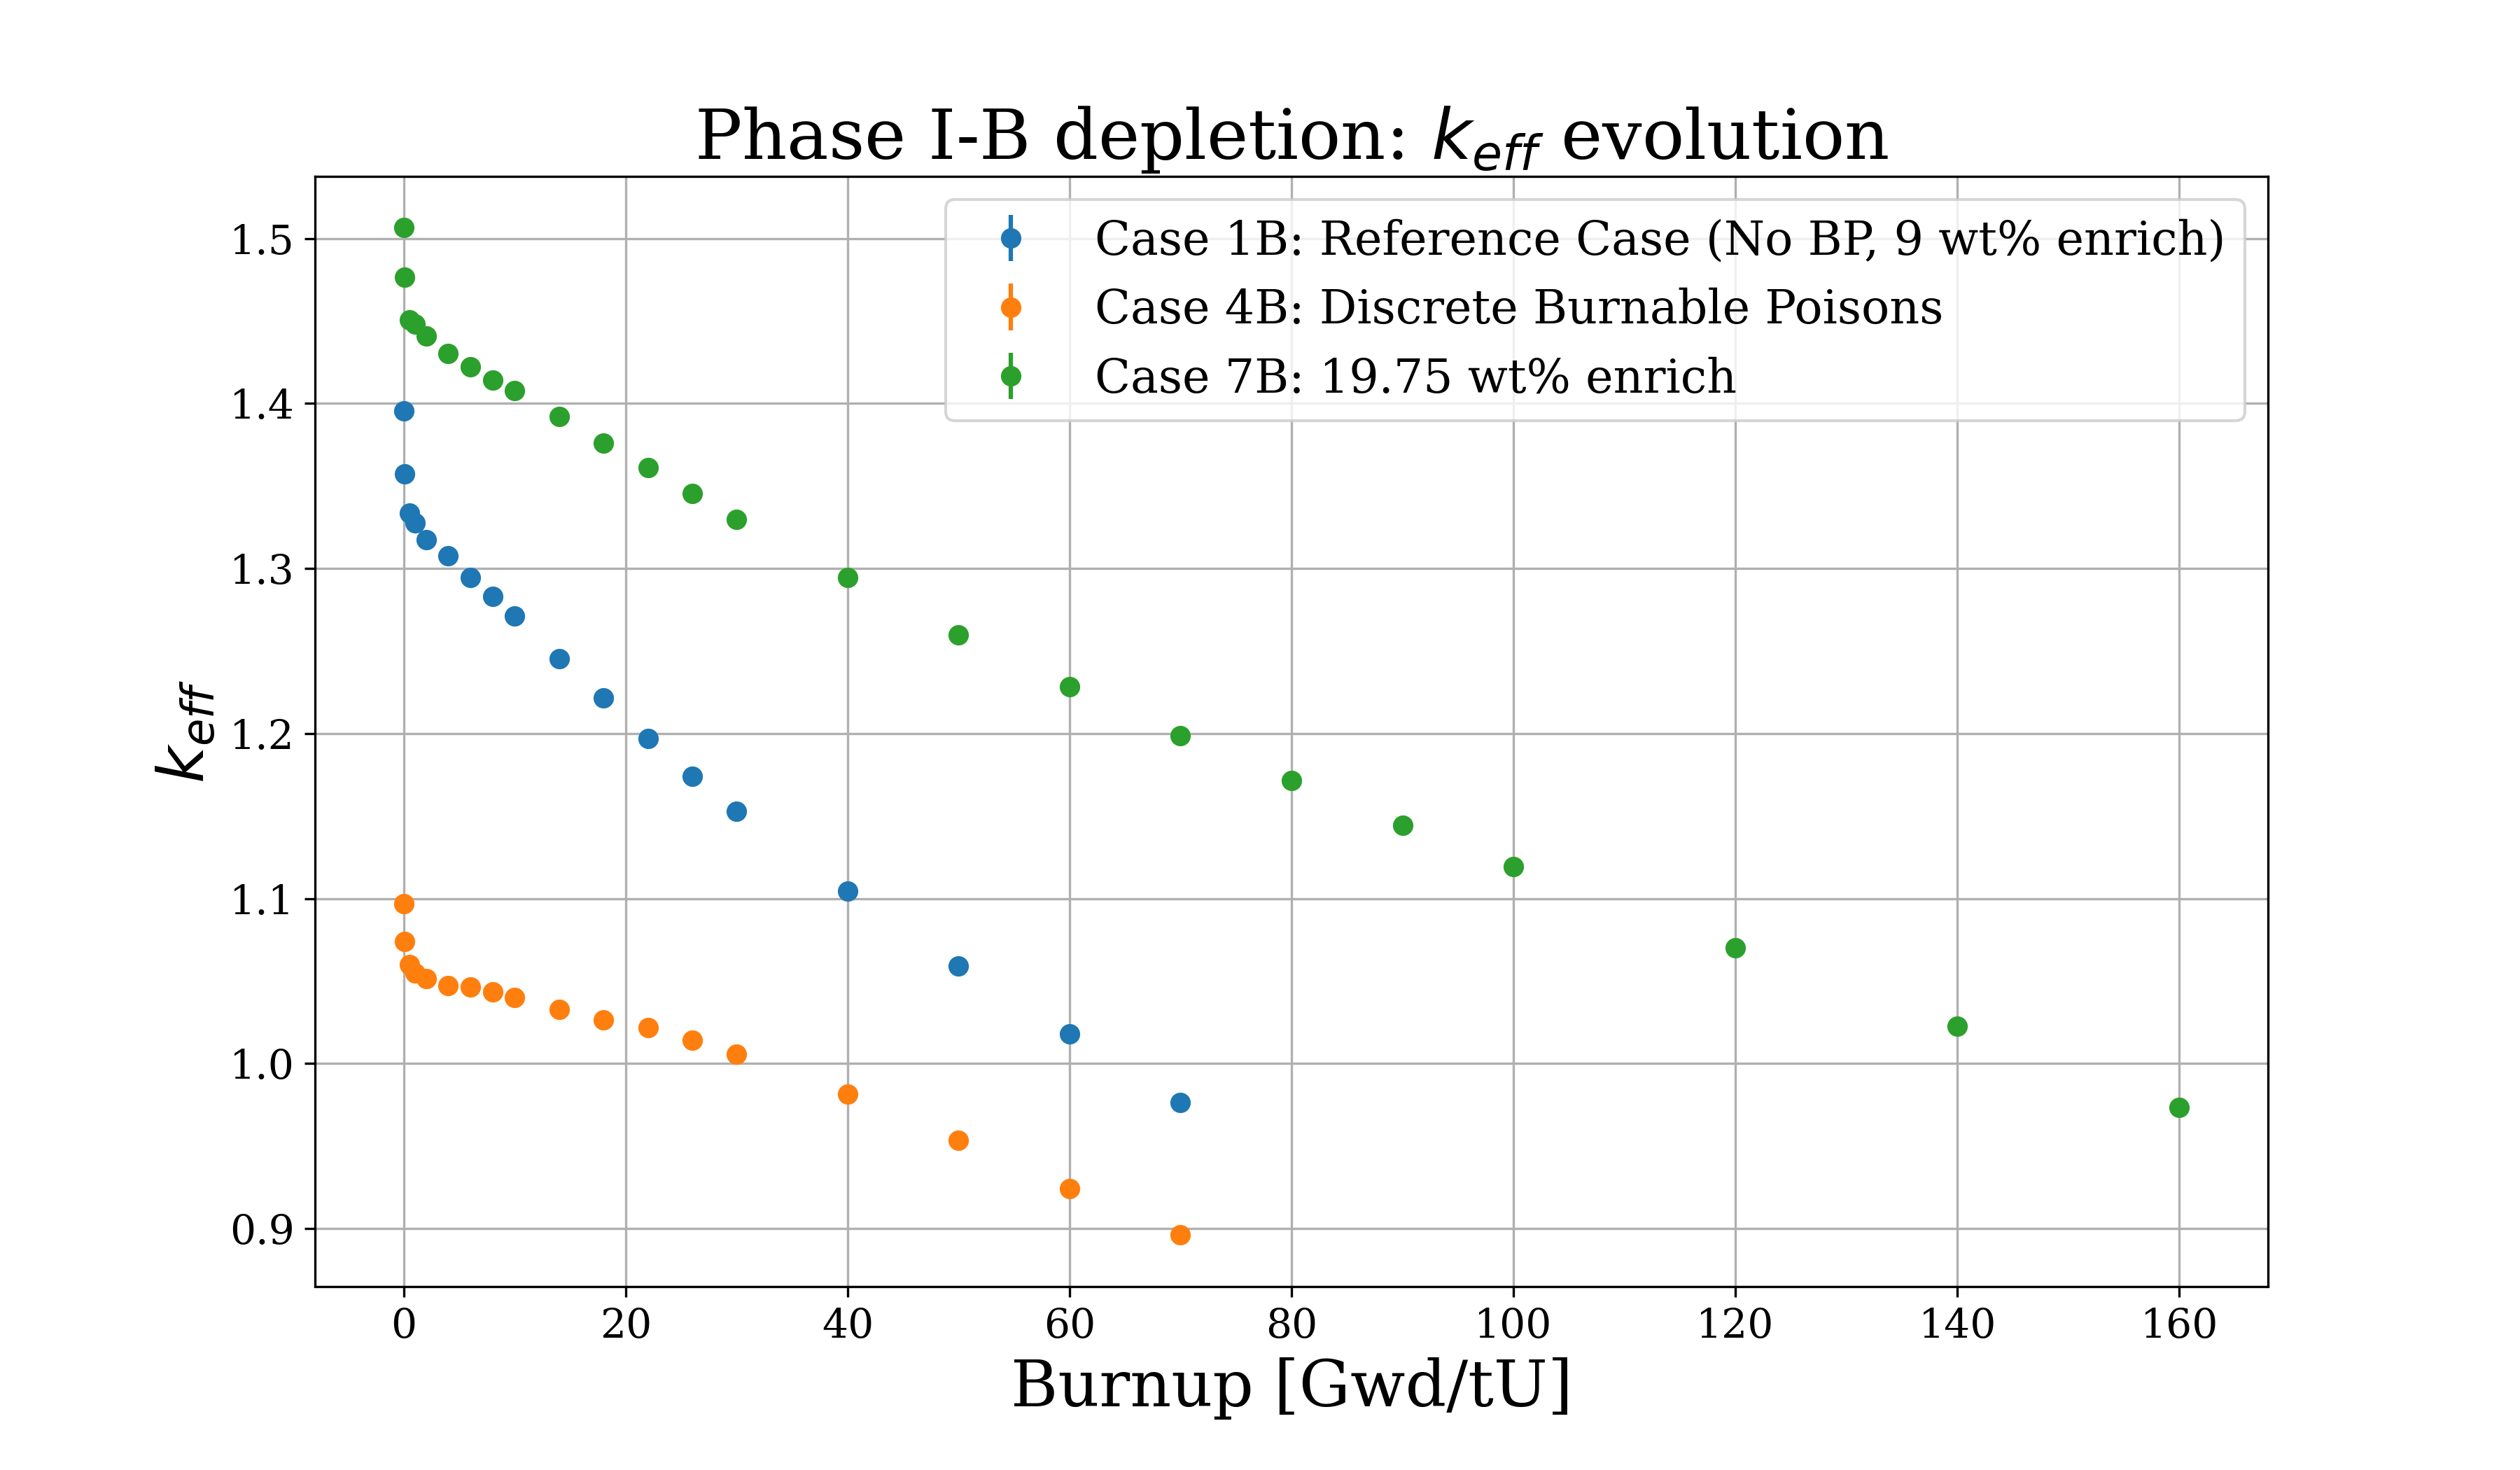
\includegraphics[width=\linewidth]{phase1b_keff.png} 
    \caption{\gls{UIUC} \gls{FHR} benchmark results: Phase I-B depletion 
    $k_{eff}$ evolution for Cases 1B, 4B, and 7B. Case 1B is the reference case, 
    Case 4B is the discrete \acrlong{BP} case, and Case 7B is the 19.75$\%$ 
    enrichment case. Error bars are included but are barely visible due to the 
    low $\sim$60pcm uncertainty.}
    \label{fig:phase1b_keff}
\end{figure}
The $k_{eff}$ at zero burnup corresponds to each case's Phase I-A $k_{eff}$ value 
reported in Table \ref{tab:phase1a-results}. 
Case 1B is the reference case with $9\%$ fuel enrichment and no \glspl{BP}. 
Case 1B's $k_{eff}$ steadily decreases until it reaches 0.967845 at the final 70 
GWd/tU burnup. 
Case 4B includes burnable poisons resulting in a lower initial $k_{eff}$. 
Case 4B's $k_{eff}$ decreases at a slower rate in the beginning due to the presence of 
burnable poisons, which decreases the flux in the core. 
At approximately 20 GWd/tU, $k_{eff}$ begins decreasing faster, presumably
due to burn-up of the poison material.   
Case 7B has a $19.75\%$ fuel enrichment, resulting in a higher initial $k_{eff}$. 
With a higher enrichment, the assembly stays critical till 140 Gwd/tU. 

\section{FHR Benchmark Temperature Model}
\label{sec:fhr-bm-temp}
I used Moltres \cite{lindsay_moltres_2017} to conduct \gls{AHTR} full assembly 
temperature simulations. 
AHTR Moltres simulations will capture thermal feedback effects absent from the purely 
neutronics OpenMC simulations conducted in the \gls{FHR} benchmark's Phase I-A.
To run Moltres simulations, the user provides group constant data from a neutron 
transport solver, such as OpenMC, for the Moltres multigroup neutron diffusion 
calculations and a mesh file representing the reactor geometry. 
In the following subsections, I will describe the steps conducted to produce the 
\gls{AHTR} temperature model with Moltres:
\begin{itemize}
    \item OpenMC neutronics model produces group constants data for the Moltres model
    \item Moltres model mesh generation
    \item Run Moltres model to calculate temperature distribution in the system 
    (Moltres model accepts group constants data and mesh) 
\end{itemize}

\subsection{FHR Benchmark: Group Constant Generation}
\label{sec:fhr-bm-group-constant}
Unlike the OpenMC neutronics model from the previous sections, Moltres does not 
explicitly model each \gls{TRISO} particle. 
Because I am using Moltres for temperature distributions and not neutron transport, 
a TRISO-level fidelity mesh file is impractical and results in extremely long Moltres 
simulation runtimes.
Instead, Moltres relies on the OpenMC model to generate group constants data
for the Moltres simulations. 
Previously, Moltres could only generate group constant data from Serpent 
\cite{leppanen_serpent_2014} or SCALE \cite{bucholz_scale:_1982} output files. 
I implemented functionality in Moltres for group constant data generation with 
OpenMC \cite{lindsay_moltres_2017}. 

To enable successful Moltres \gls{AHTR} temperature model simulations, I established 
suitable spatial and energy homogenization for group constant generation.
These homogenizations preserve accuracy while maintaining an acceptable runtime.
I used eight precursor groups and a four-group energy structure derived by Gentry et al. 
\cite{gentry_development_2016} for \gls{AHTR} geometries.
Table \ref{tab:energy_structures-bm} defines the 4-group energy boundaries. 
\begin{table}[htbp]
    \centering
    \onehalfspacing
    \caption{4-group energy structures for \acrfull{AHTR} geometry 
    derived by Gentry et al. \cite{gentry_development_2016}.}
	\label{tab:energy_structures-bm}
    \footnotesize
    \begin{tabular}{lll}
    \hline
    \multicolumn{3}{c}{\textbf{Group Boundaries [MeV]}} \\ 
    \hline
    \textbf{Group $\#$}& \textbf{Upper Bound} & \textbf{Lower Bound}  \\
    \hline 
    1 & $2.0000\times 10^1$ & $9.1188\times 10^{-3}$ \\ 
    2 & $9.1188\times 10^{-3}$ & $2.9023\times 10^{-5}$\\
    3 & $2.9023\times 10^{-5}$ & $1.8554\times 10^{-6}$\\
    4 & $1.8554\times 10^{-6}$ & $1.0000\times 10^{-12}$\\
    \hline
    \end{tabular}
\end{table}
For spatial homogenization of the \gls{AHTR} fuel assembly, I used OpenMC's \textit{cell} 
domain type to compute multigroup cross sections for different \textit{cells}.
I discretized the fuel assembly into 61 \textit{cells}: inter-assembly \gls{FLiBe}, Y-shaped 
graphite structure, control rod slot \gls{FLiBe}, graphite spacers, each diamond shape section's 
inter-plank \gls{FLiBe} (3), each graphite plank (18), and each fuel stripe (36).
I used reflective boundary conditions.
Figure \ref{fig:assembly_mg} illustrates the \gls{AHTR} assembly's spatial 
homogenization used for group constant generation.
\begin{figure}[htbp]
    \centering
    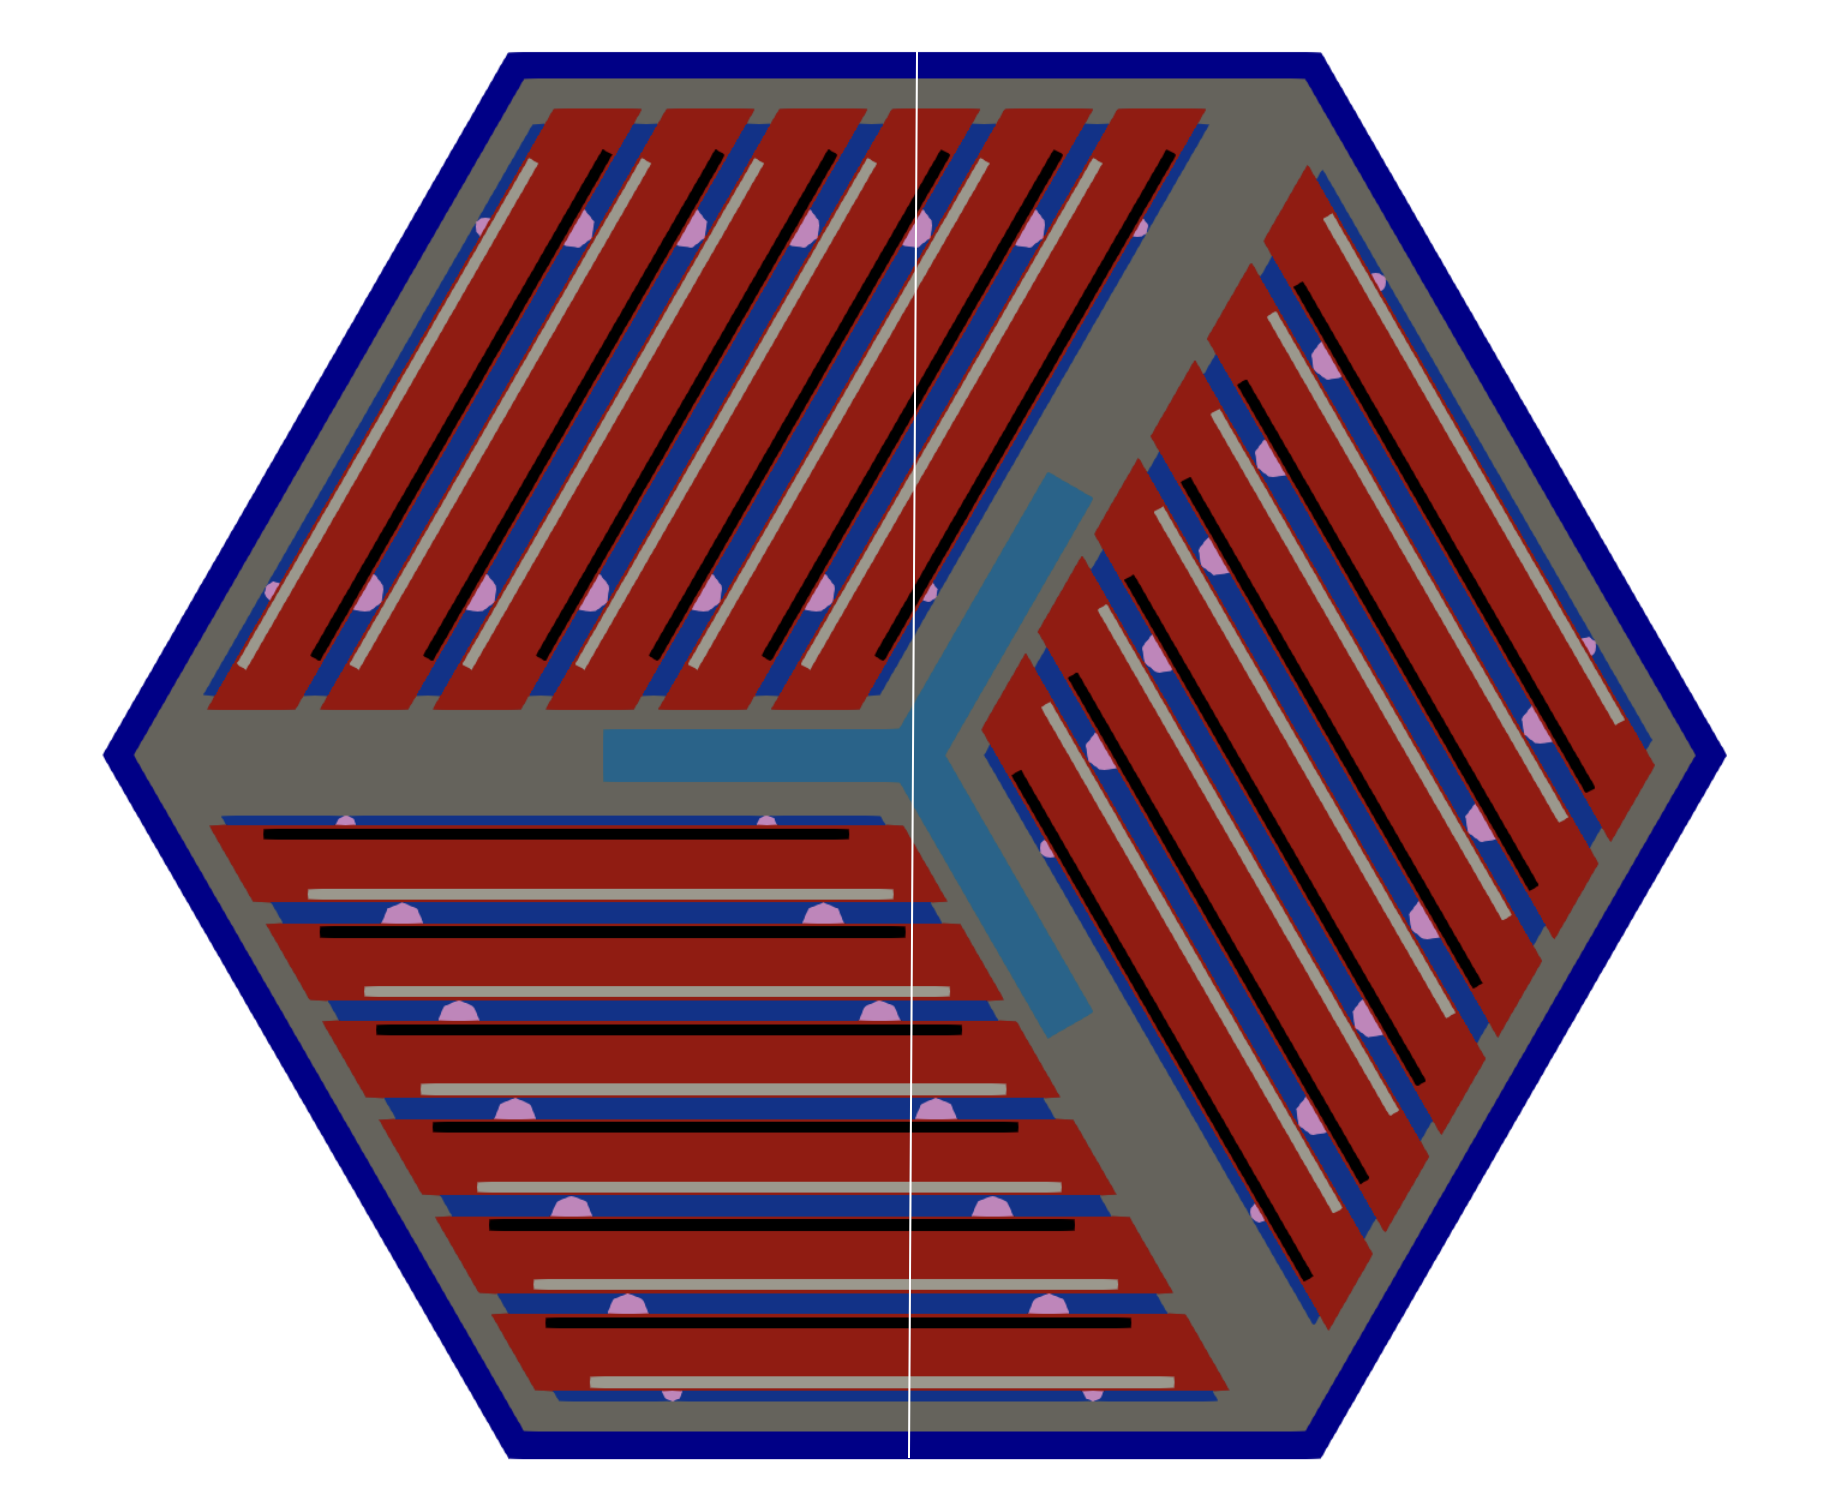
\includegraphics[width=\linewidth]{assembly_mg.png}
    \raggedright
    \resizebox{0.5\textwidth}{!}{
        \hspace{1cm}
        \fbox{\begin{tabular}{ll}
            \textcolor{fhrblue1}{$\blacksquare$} & inter-assembly \gls{FLiBe} \\
            \textcolor{fhrgrey1}{$\blacksquare$} & Y-shaped graphite structure \\
            \textcolor{fhrblue2}{$\blacksquare$} & control rod slot \gls{FLiBe} \\
            \textcolor{fhrblue3}{$\blacksquare$} & inter-plank \gls{FLiBe} \\
            \textcolor{fhrpink1}{$\blacksquare$} & spacers \\
            \textcolor{fhrred1}{$\blacksquare$} & graphite planks \\
            \textcolor{fhrblack1}{$\blacksquare$} \textcolor{fhrwhite1}{$\blacksquare$} & fuel stripes
            \end{tabular}}}
    \caption{\acrfull{AHTR} assembly spatially discretized into 
    61 \textit{cells} for OpenMC multigroup calculation to produce group constants 
    data for the Moltres model.
    61 \textit{cells}: inter-assembly \gls{FLiBe}, Y-shaped graphite structure, control 
    rod slot \gls{FLiBe}, graphite spacers, each diamond shape section's inter-plank 
    \gls{FLiBe} (3), each graphite plank (18), and each fuel stripe (36).
     The white line corresponds to the centerline where flux distribution is measured.}
    \label{fig:assembly_mg}
\end{figure}

With the above-described energy discretization and spatial homogenization, I generated 
group constants with Moltres using four OpenMC simulations at 948K, 1024K, 1100K, and 
1200K. 
The OpenMC simulations are run with 80 active cycles, 20 inactive cycles, and 8000 
particles resulting in an uncertainty of $\sim 150pcm$.
In the next subsection, I compare the key neutronics parameters for the continuous 
OpenMC and multigroup Moltres simulations for the \gls{AHTR} assembly at 948K to 
ensure that the spatial homogenization and energy discretization preserve accuracy. 

\subsubsection{FHR Benchmark: Key Neutronics Parameters Verification}
In this section, I verify that the spatial homogenization and energy discretization 
I chose are acceptable by verifying key neutronics parameters.
I compare the key neutronics parameters between two simulations:
\begin{enumerate}
    \item OpenMC simulation with continuous energy and TRISO-level spatial fidelity 
    \item Moltres simulation with 4-group energy and spatial homogenization
\end{enumerate}
All materials' in the OpenMC simulation are 948K. 
The OpenMC simulation with TRISO-level fidelity generates the group constants for the 
energy and spatially homogenized Moltres simulation. 
I compare the following key neutronics parameters: effective multiplication factor, 
reactivity coefficients, flux distribution, and neutron energy spectrum. 
The comparisons are to verify that the Moltres model is replicating the OpenMC 
model's neutronics correctly.
And of these, comparisons of the reactivity coefficients and flux distributions 
are key to ensuring that Moltres accurately calculates the \gls{AHTR}'s 
temperature distribution.
The reactivity coefficients capture temperature reactivity feedback on the flux 
when the temperature varies with space in the Moltres model. 
The heat produced per fission, $\epsilon_{f,g}$, and macroscopic cross section 
for fission, $\Sigma_{f,g}$, terms in the Moltres source term (Equation 
\ref{eq:moltres-source-term}) are provided to Moltres through 
the group constants generated by the transport software, OpenMC.
Thus, differences in the source term between OpenMC and Moltres are dependent on 
the flux. 

\paragraph{Effective Multiplication Factor}
Comparing $k_{eff}$ and reactivity produced by Moltres and OpenMC verify that the 
Moltres model replicates the OpenMC model's neutronics correctly.
Table \ref{tab:keff_assem_comparison} compares the effective multiplication factor 
($k_{eff}$) and reactivity ($\rho$)
for OpenMC simulation with continuous energy and TRISO-level spatial fidelity, 
OpenMC simulation with 4-group energy and spatial homogenization, 
and Moltres simulation with 4-group energy and spatial homogenization.
I include results from the homogenized OpenMC simulation to 
distinguish between differences caused by spatial homogenization and energy 
discretization or differing OpenMC and Moltres solve methods. 
\begin{table}[htbp]
    \centering
    \onehalfspacing
    \caption{\acrfull{AHTR} assembly's $k_{eff}$ and reactivity values from the 
    OpenMC simulation with continuous energy and TRISO-level spatial fidelity, 
    OpenMC simulation with 4-group energy and spatial homogenization, and Moltres 
    simulation with 4-group energy and spatial homogenization. 
    All simulations are at 948K.
    The normalized difference is the pcm difference normalized by OpenMC non-homogenized 
    model's $k_{eff}$.}
	\label{tab:keff_assem_comparison}
    \footnotesize
    \begin{tabular}{lllclc}
    \hline 
    \textbf{Software}& \textbf{Homogenized?}& \textbf{$k_{eff}$} & \textbf{Diff [pcm]}  
    & \textbf{Reactivity [pcm]} & \textbf{Reactivity Diff [pcm]} \\
    \hline 
    OpenMC & No & $1.39850 \pm 0.00126$ & - & $28495 \pm 64$ & - \\ 
    OpenMC & Yes & $1.398373 \pm 0.00115$ & \Minus13 & $28488 \pm 58$ & \Minus6\\ 
    Moltres & Yes & $1.40273 $ & \Plus423 & 28710 & \Plus 216\\ 
    \hline
    \end{tabular}
\end{table}

The $13pcm$ $k_{eff}$ and $6pcm$ reactivity difference, that can be observed in Table 
\ref{tab:keff_ahtr_moltres}, between continuous and homogenized OpenMC simulations 
are within uncertainty.
This shows that the selected spatial homogenizations and energy discretizations 
are acceptable. 
However, the Moltres simulation shows a $423pcm$ difference in $k_{eff}$ and 
$216pcm$ difference in reactivity.
The summary at the end of this section explains the differences in these values. 

\paragraph{Reactivity Coefficients}
A comparison of reactivity coefficients produced by Moltres and OpenMC verifies 
that the Moltres model is replicating the OpenMC model's neutronics correctly and 
are also important to ensure that Moltres accurately calculates the temperature 
distribution.
Moltres' delayed neutron fraction, $\beta{eff}$, is calculated by taking the 
normalized difference between $k_{eff}$ values with and without \glspl{DNP}. 
Table \ref{tab:ahtr_full_assem_moltres_coeffs} shows that the $\beta{eff}$ values from 
OpenMC and Moltres show excellent agreement with a discrepancy of 0.84pcm. 
I calculated the temperature reactivity coefficients using Equation 
\ref{eq:reactivity-coefficient}.
Temperature reactivity feedback arises mainly from Doppler broadening of 
resonance absorption peaks and thermal expansion.
Table \ref{tab:ahtr_full_assem_moltres_coeffs} also shows that the total temperature 
coefficients from OpenMC and Moltres have good agreement with a discrepancy of 
0.43 $pcm \cdot K^{-1}$.
\begin{table}[htbp]
    \centering
    \onehalfspacing
    \caption{\acrfull{AHTR} assembly's $\beta_{eff}$ values from OpenMC and Moltres 
    simulations at 948K and total reactivity coefficient values calculated from 
    OpenMC and Moltres at 948K and 1100K.
    The OpenMC simulation has continuous energy and TRISO-level spatial fidelity, and the
    Moltres simulation has 4-group energy and spatial homogenization.}
    \footnotesize
	\label{tab:ahtr_full_assem_moltres_coeffs}
    \begin{tabular}{llllll}
    \hline 
    \textbf{Software}& \textbf{Homogenized?}& \textbf{$\beta_{eff}$ [pcm]} 
    & \textbf{Diff [pcm]} & \textbf{Total $\frac{\Delta \rho}{\Delta T}$ [$pcm \cdot K^{-1}$]} 
    & \textbf{Diff [$pcm \cdot K^{-1}$]} \\
    \hline 
    OpenMC & No &  653.40 & - &  \Minus3.63 & - \\ 
    Moltres & Yes & 652.57 & \Minus0.84 & \Minus4.06 & \Minus0.43\\ 
    \hline
    \end{tabular}
\end{table}

\paragraph{Flux Distribution}
A comparison of flux distributions produced by Moltres and OpenMC verifies that the 
Moltres model is replicating the OpenMC model's neutronics correctly and are also 
important to ensure that Moltres accurately calculates the temperature distribution.
Figure \ref{fig:flux_948K_full_assem} shows the 4-group flux distributions for OpenMC and 
Moltres models' on the \gls{AHTR} assembly's centerline, along the y-axis at 
the x-axis' midpoint (white line on Figure \ref{fig:assembly_mg}). 
\begin{figure}[htbp]
    \centering
    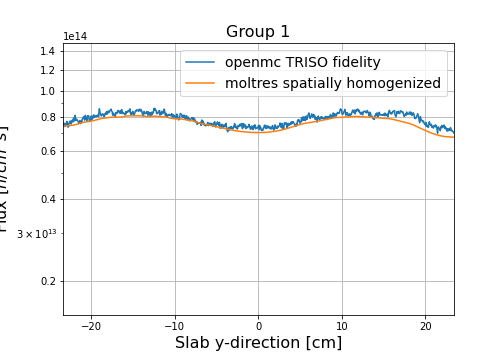
\includegraphics[width=0.48\linewidth]{flux_group1_948K_full_assem.png} 
    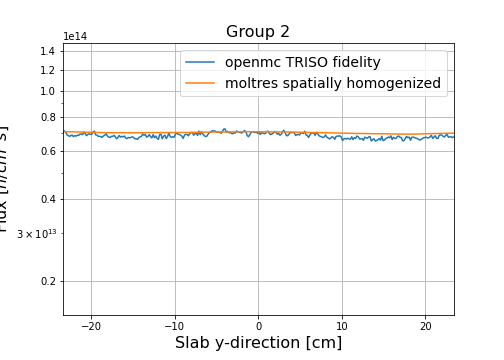
\includegraphics[width=0.48\linewidth]{flux_group2_948K_full_assem.png} 
    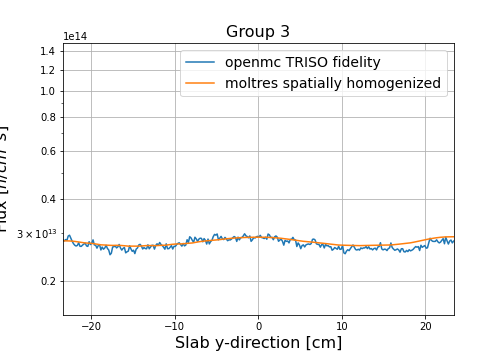
\includegraphics[width=0.48\linewidth]{flux_group3_948K_full_assem.png} 
    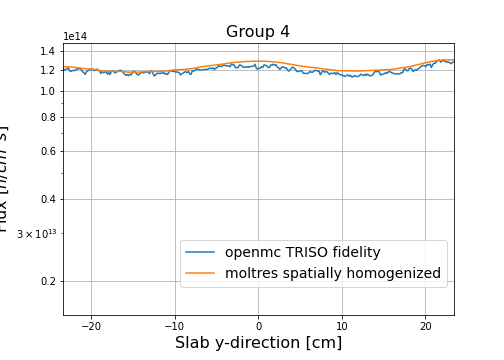
\includegraphics[width=0.48\linewidth]{flux_group4_948K_full_assem.png} 
    \caption{\acrfull{AHTR} assembly's centerline neutron flux distribution 
    in 4 groups at 948K (discretized into 1000 points). 
    Centerline is the white line in Figure \ref{fig:assembly_mg}.
    Comparison is between OpenMC simulation with continuous energy 
    and TRISO-level spatial fidelity and Moltres simulation with 4-group energy and 
    spatial homogenization.
    Energy Group 1: E $> 9.1188 \times 10^{-3}$ MeV, 
    Energy Group 2: $2.9023 \times 10^{-5} < E < 9.1188 \times 10^{-3}$ MeV,
    Energy Group 3:  $1.8556 \times 10^{-5} < E < 2.9023 \times 10^{-5}$ MeV,
    Energy Group 4:  $1.0 \times 10^{-12} < E < 1.8554 \times 10^{-6}$ MeV.}
    \label{fig:flux_948K_full_assem}
\end{figure}
Table \ref{tab:ahtr-full-assem-verification-flux} reports the 2-norm percentage 
difference (Equation \ref{eq:ahtr-assem-flux-2norm}) and maximum percentage 
difference between centerline flux values from OpenMC and Moltres models. 
\begin{align}
    \label{eq:ahtr-assem-flux-2norm}
    ||\Delta \phi||_N &= \frac{1}{N}\sqrt{\sum_{i=1}^N(\frac{\phi_{moltres, i} - \phi_{openmc, i}}{\phi_{openmc, i}}\times100)^2} \\
\intertext{where}
    ||\Delta \phi||_N &= \mbox{normalized 2-norm flux percentage difference between Moltres and OpenMC } [\%] \nonumber \\
    N &= \mbox{total number of discretized points} \nonumber \\
    \phi_{moltres} &= \mbox{Moltres model's centerline flux } [\frac{n}{cm^2s}] \nonumber \\
    \phi_{openmc} &= \mbox{OpenMC model's centerline flux } [\frac{n}{cm^2s}] \nonumber 
\end{align} 
\begin{table}[htbp]
    \centering
    \onehalfspacing
    \caption{\acrfull{AHTR} assembly's centerline normalized 2-norm of flux percentage 
    difference and maximum flux percentage difference. 
    Centerline is the white line in Figure \ref{fig:assembly_mg}.
    The difference values are calculated from comparison between the OpenMC simulation with 
    continuous energy and TRISO-level spatial fidelity and Moltres simulation with 4-group energy 
    and spatial homogenization.}
	\label{tab:ahtr-full-assem-verification-flux}
    \footnotesize
    \begin{tabular}{lll}
    \hline 
    \textbf{Energy Group}& \textbf{2-norm difference [$\%$]}& \textbf{Max difference [$\%$]} \\
    \hline 
    1 & 0.13 & \Minus10.57 \\
    2 & 0.08 & \Plus7.58 \\
    3 & 0.10 & \Plus8.96 \\
    4 & 0.09 & \Plus6.97 \\
    \hline
    \end{tabular}
\end{table}

Figure \ref{fig:flux_948K_full_assem} shows that the OpenMC model has good flux 
agreement for all groups. 
Table \ref{tab:ahtr-plank-verification-flux} shows that the 2-norm percentage differences 
between OpenMC and Moltres models' flux values are slight, demonstrating a 
good overall agreement for each group's flux.
The summary at the end of this section explains the differences in the flux's maximum 
percentage differences between the OpenMC and Moltres models. 
%The large maximum percentage difference in flux values in Group 2 and 3 is attributed to 
%their resonance regions, causing large one-off differences at some discretized points.
%The flux neutronics parameter is most important as it contributes to the source term in the 
%Moltres simulation. 
%Thus, these accurate flux comparison results verify the accurate calculation 
%of the temperature distribution in the Moltres \gls{AHTR} full assembly model. 

\paragraph{Neutron Energy Spectrum}
Figure \ref{fig:neutron_spectrum_948K_full_assem} shows the neutron spectrum of the 
OpenMC simulation for both 252 and 4 groups and the 4-group Moltres simulation.
 \begin{figure}[htbp]
    \centering
    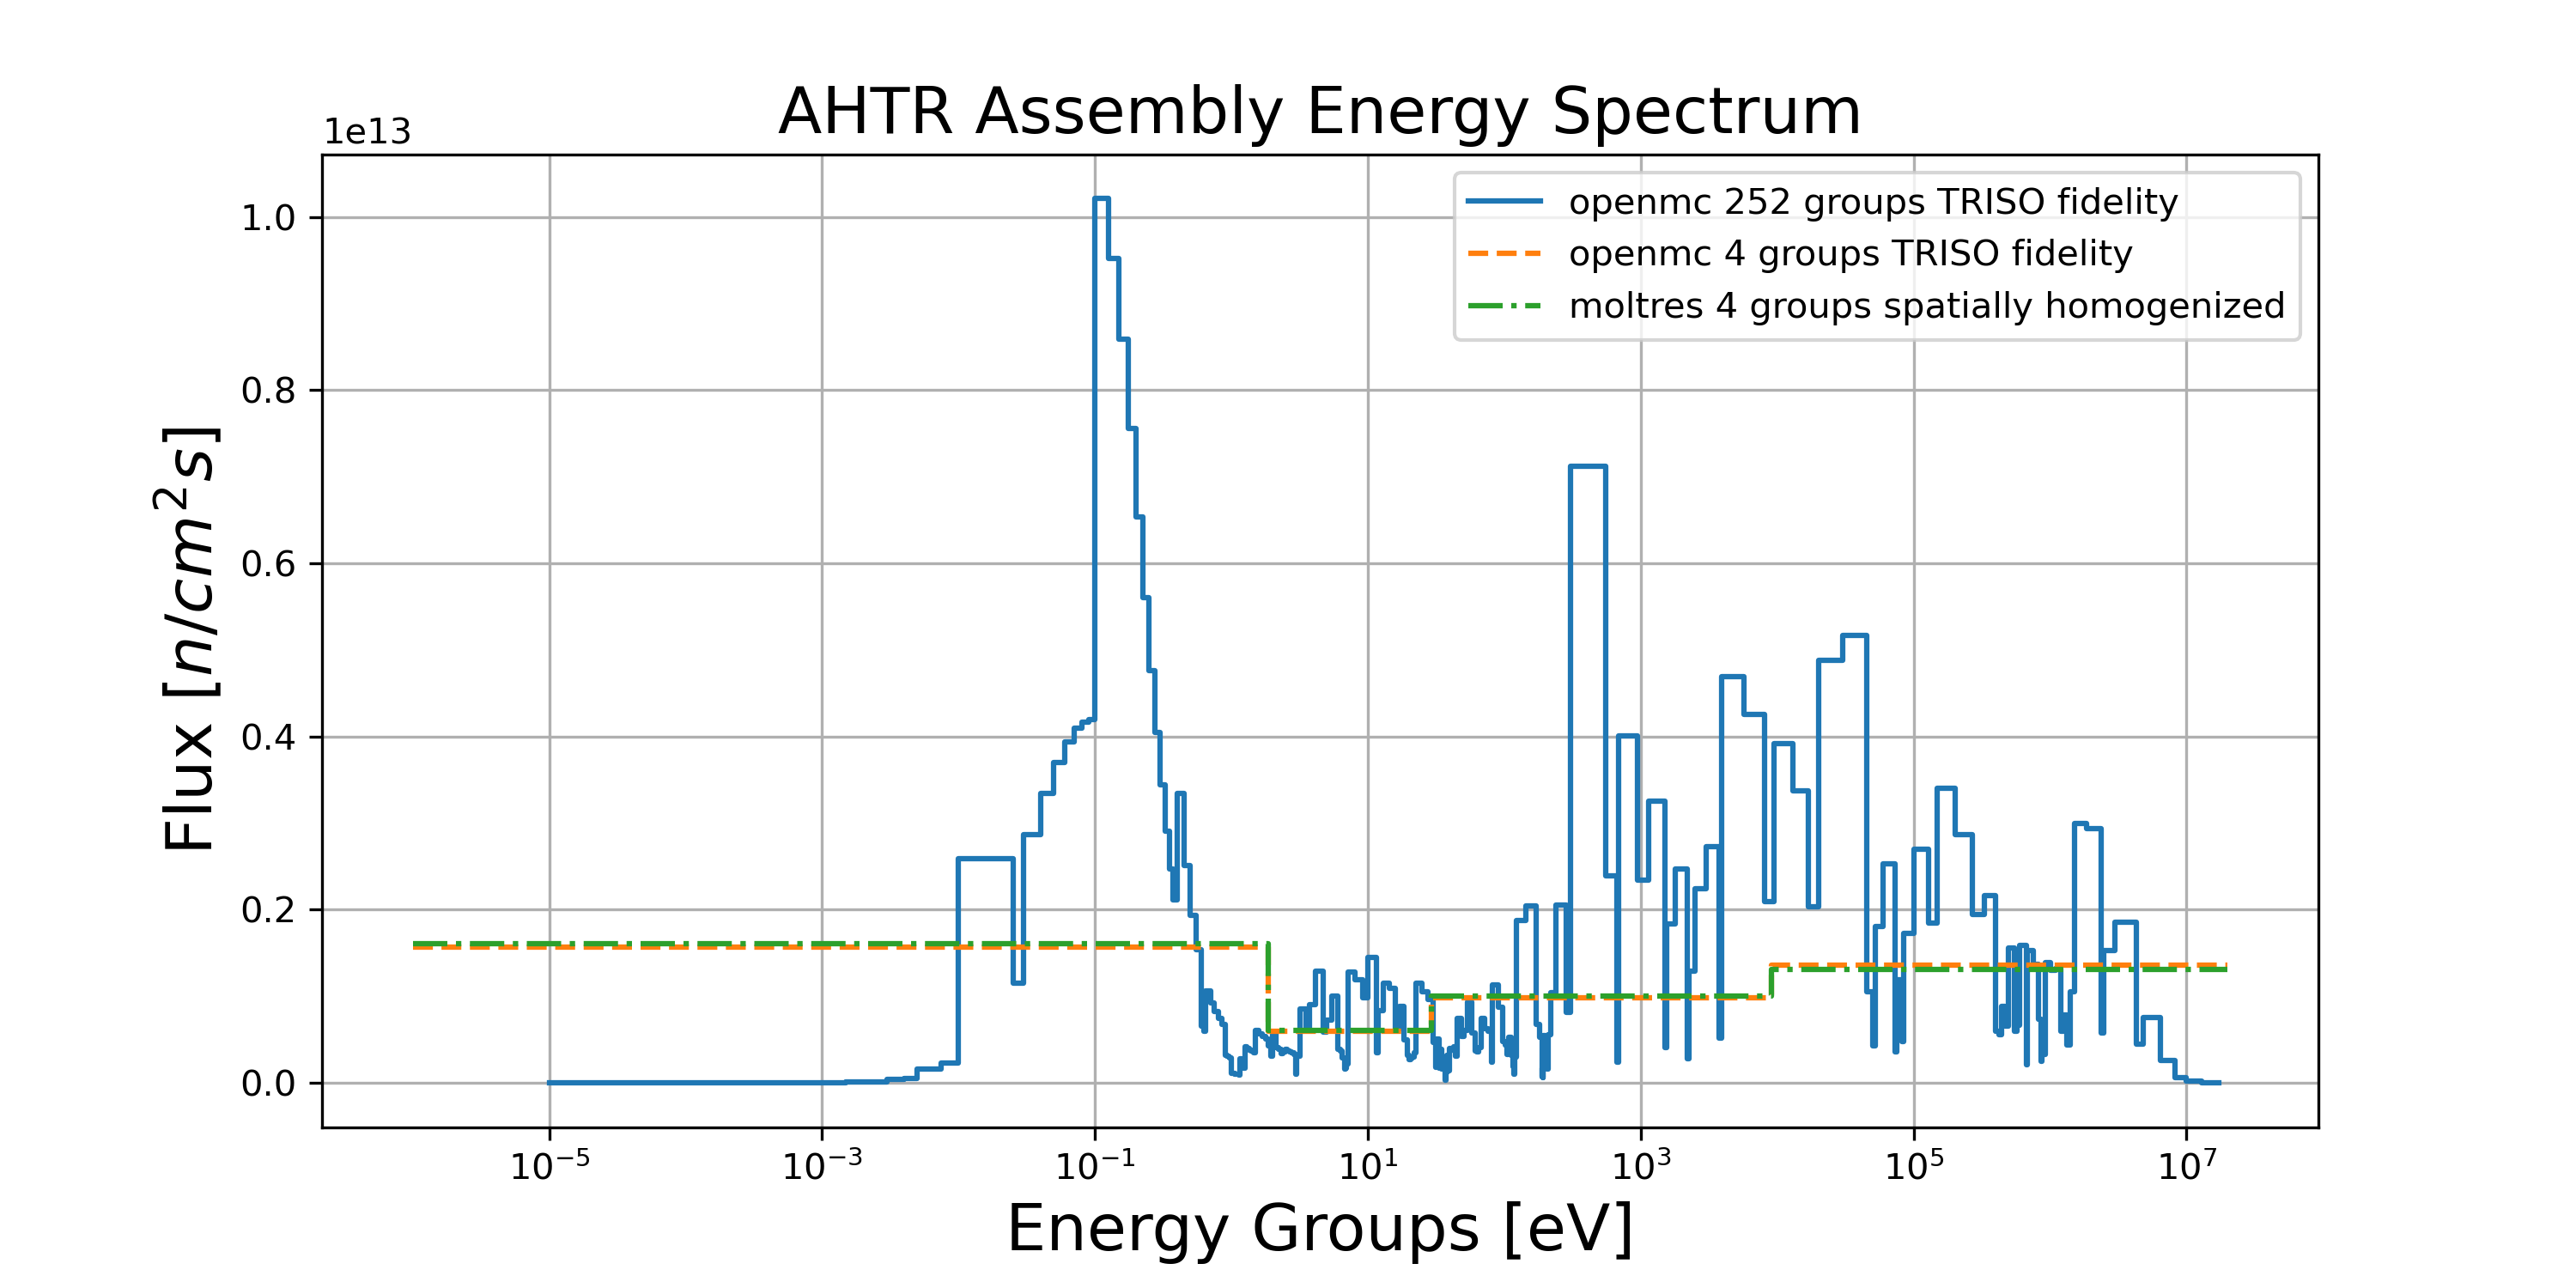
\includegraphics[width=\linewidth]{neutron_spectrum_948K_full_assem.png}
    \caption{\acrfull{AHTR} full assembly's neutron spectrum. Spectrums include 252 
    and 4 group spectrums from OpenMC simulation with continuous energy and 
    TRISO-level spatial fidelity and 4 group spectrum from Moltres simulation with 
    4-group energy and spatial homogenization.}  
    \label{fig:neutron_spectrum_948K_full_assem}
\end{figure}
There is good agreement between OpenMC and Moltres models 4-group spectrums. 

\subsubsection{Key Neutronics Parameters Verification Summary}
% todo: edits to make this more correct for the fhr benchmark. 
The verification study found a 216 pcm reactivity difference between OpenMC 
and Moltres models and good agreement in their reactivity coefficients and 4-group 
neutron energy spectrum.
The verification study also found good agreement in overall flux distributions 
(based on the 2-norm difference); however, there were larger flux differences at 
specific points. 
The reactivity and flux differences are due to Moltres utilizing the neutron
diffusion method instead of neutron transport methods, resulting in flux not 
being reproduced well in small regions which are less than a few mean free paths 
in length (i.e., the FLiBe coolant channel has 0.7cm which is smaller than 
the diffusion coefficient). 
The differences in reactivity and flux at specific points might result in a 
slightly inaccurate absolute temperature distribution.  
However, since the reactivity coefficients and overall flux distribution are in 
agreement, Moltres accurately captures the relative temperature distributions. 
During the \gls{AHTR} optimization, so long the relative maximum temperature between 
different \gls{AHTR} models is captured correctly, \gls{ROLLO} can find optimal reactor 
geometries accurately. 
Reactor designers can then use higher fidelity software for modeling the final optimal 
\gls{AHTR} geometry. 
In summary, Moltres replicated the relevant neutronics parameters with sufficient 
accuracy using OpenMC's group constant data for the \gls{AHTR} full assembly 
model. 

\subsection{FHR Benchmark: Moltres Mesh Generation}
I created an \gls{AHTR} assembly geometry file (\texttt{.geo}) based on the spatial 
homogenization described in Section \ref{sec:fhr-bm-group-constant}.
The \gls{AHTR} mesh is then generated from the geometry file using Gmsh 
\cite{geuzaine_gmsh_2009}.
I used Gmsh's \textit{refine by splitting} functionality to refine the mesh.
Figure \ref{fig:ahtr-full-assem-geo} shows the \gls{AHTR} assembly's Gmsh rendered 
geometry file.
\begin{figure}[htbp]
    \centering
    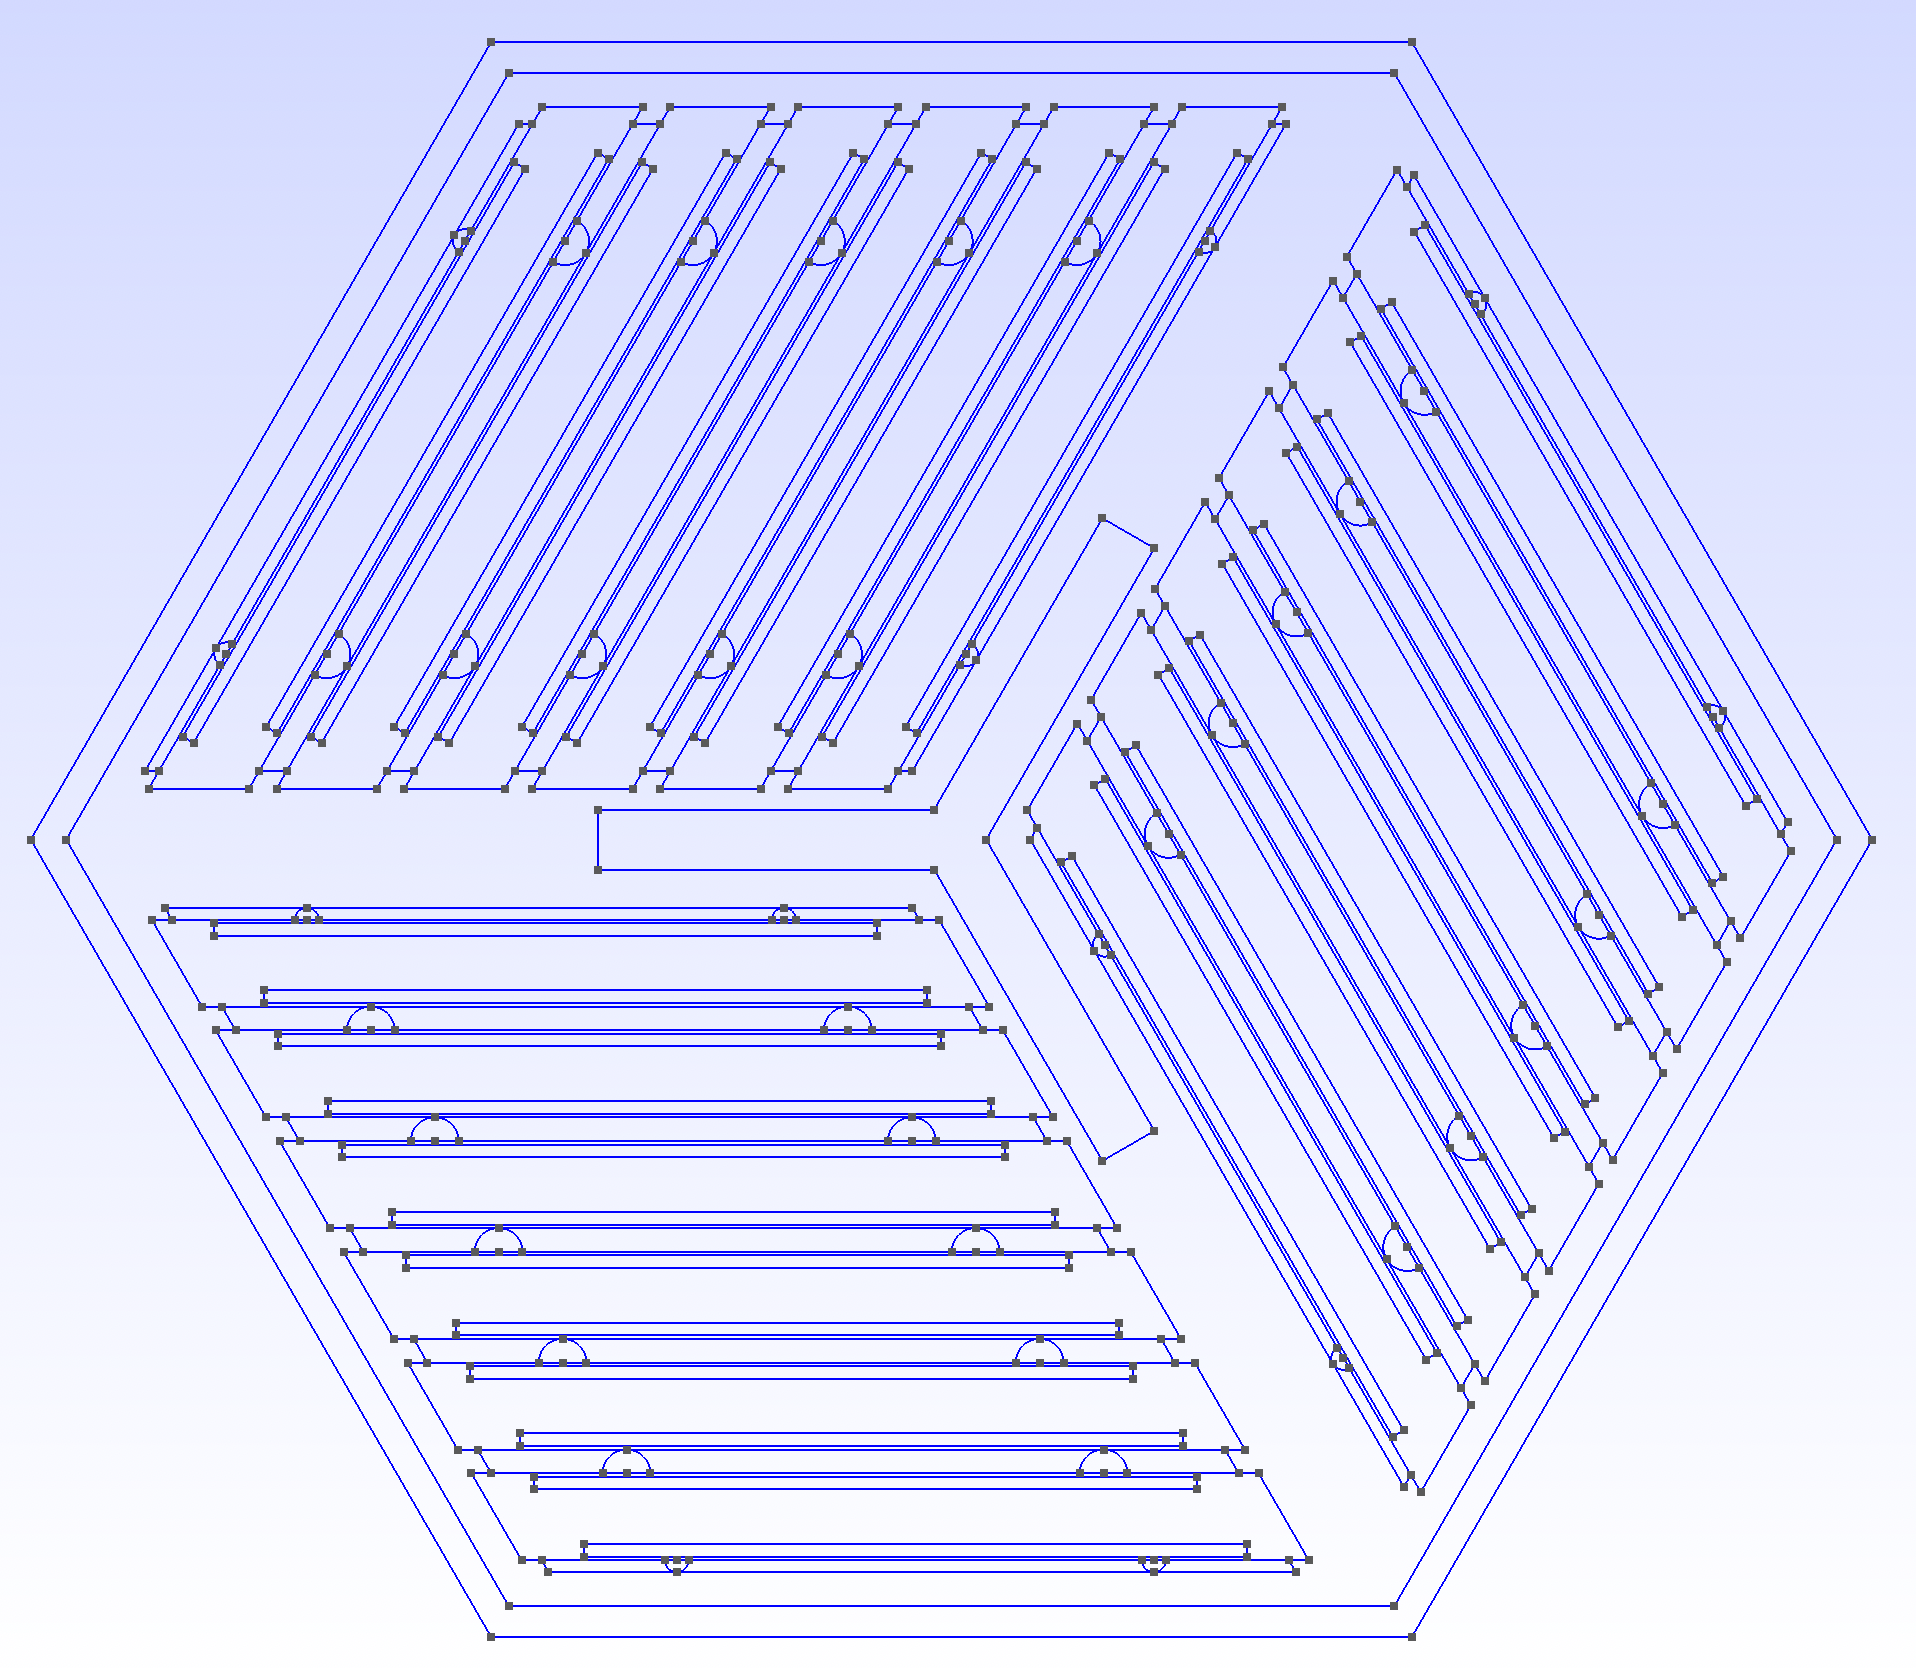
\includegraphics[width=\linewidth]{ahtr-full-assem-geo.png}
    \caption{\acrfull{AHTR} assembly's Gmsh rendered geometry file. 
    I meshed the geometry file using Gmsh.
    The mesh file is used in the \gls{AHTR} assembly Moltres temperature model.}
    \label{fig:ahtr-full-assem-geo}
\end{figure}

\pagebreak
\subsubsection{FHR Benchmark: Mesh Refinement Study}
I performed a mesh refinement study on the \gls{AHTR} full assembly Moltres temperature 
model to ensure that the geometry mesh inputs are sufficiently converged. 
Table \ref{tab:ahtr-full-assem-mesh-refinement} reports the average, maximum, and 
normalized 2-norm of discretized temperature difference between refinement steps 
(Equation \ref{eq:2-norm-tdiff-i-full-assem}):
\begin{align}
    \label{eq:2-norm-tdiff-i-full-assem}
    ||\Delta T_k||_N &= \frac{1}{N}\sqrt{\sum_{i=1}^N(T_{k-1, i} - T_{k, i})^2 }\\
\intertext{where}
    ||\Delta T_k||_N &= \mbox{normalized 2-norm discretized temperature difference 
    between refinement steps } [K]\nonumber \\
    N &= \mbox{total number of discretized points} \nonumber \\
    k &= \mbox{refinement step} \nonumber \\
    T_{k-1} &= \mbox{temperatures from previous refinement step } [K]\nonumber \\
    T &= \mbox{temperatures from current refinement step } [K]\nonumber 
\end{align} 
\begin{table}[htbp]
    \centering
    \onehalfspacing
    \caption{\acrfull{AHTR} full assembly's Moltres temperature model's mesh refinement study.}
	\label{tab:ahtr-full-assem-mesh-refinement}
    \footnotesize
    \begin{tabular}{lp{3.5cm}lp{3.5cm}ll}
        \hline 
        \textbf{Refinement} & \textbf{Max Assembly Temp [K]} 
        & \textbf{Diff [K]} & \textbf{Ave Assembly Temp [K]}
        & \textbf{Diff [K]} & $||\Delta T_k||_N$ [K]\\ 
        \hline 
        1 & 1040.931 & - & 960.619 & - & -\\
        2 & 1048.941 & \Plus8.010 & 962.854 & \Plus2.235 & 0.175\\
        3 & 1057.403 & \Plus8.463 & 963.948 & \Plus1.093 & 0.067\\
        4 & 1061.599 & \Plus4.196 & 965.020 & \Plus1.073 & 0.053\\
        \hline
    \end{tabular}
\end{table}

The mesh refinement study shows suitable $||\Delta T_k||_N$ convergence with more 
refinement steps. 
Therefore, I used x4 mesh refinement for the \gls{AHTR} full assembly Moltres 
temperature model. 

\subsection{FHR Benchmark: Temperature Model}
\label{sec:fhr-benchmark-temp-model}
The Moltres \gls{AHTR} steady-state temperature model is a 2D x-y cross-section 
model of the \gls{AHTR} assembly. 
The Moltres temperature model first solves the \gls{AHTR} neutronics and uses that to 
solve the \gls{AHTR}'s temperature distribution for a defined power.
The temperature model assumes conductive heat transfer throughout the domain 
and heat removal by uniform salt flow in the coolant regions. 
These assumptions ignore turbulent effects that would most likely be present. 
However, an in-depth AHTR Moltres model that includes turbulence modeling is 
out of scope for this dissertation. 

\subsubsection{FHR Benchmark: Temperature Model Setup}
Moltres solves the four-group diffusion equations 
(Equation \ref{eq:moltres-diffusion-equation}) 
as a steady-state eigenvalue problem to find $k_{eff}$ for the static \gls{AHTR} models.
In the 2D cross-sectional \gls{AHTR} steady-state temperature model, I ignore the 
time-dependent and velocity-dependent terms from Moltres' temperature governing 
equation (Equation \ref{eq:moltres-temp}) since it is a steady-state model with
no moving fuel, resulting in Equation \ref{eq:moltres-temp-ss-bm}: 
\begin{align}
    \label{eq:moltres-temp-ss-bm}
    - \nabla \cdot (k_i \nabla T) &= Q_i
\intertext{where}
k_i &= \mbox{thermal conductivity of material i} \nonumber \\
T &= \mbox{temperature in the model} \nonumber \\
Q_i &= \mbox{source or sink term in material i} \nonumber
\end{align} 
I use insulated temperature boundary conditions.  
Table \ref{tab:ahtr-thermal-conductivity-bm} shows the thermal conductivity values 
used for each \gls{AHTR} material. 
\begin{table}[htbp]
    \centering
    \onehalfspacing
    \caption{\acrfull{AHTR} materials' thermal conductivities used in Moltres 
    temperature models, taken from \cite{ramey_methodology_2021}.}
	\label{tab:ahtr-thermal-conductivity-bm}
    \footnotesize
    \begin{tabular}{ll}
    \hline 
    \textbf{Material}& \textbf{Thermal Conductivity} \\
    & [$Wcm^{-1}K^{-1}$] \\ 
    \hline 
    \gls{FLiBe} & 0.01 \\
    Graphite  & 0.15 \\
    Fuel  & 0.099 \\
    \hline
    \end{tabular}
\end{table}

Equation \ref{eq:moltres-source-term-bm} defines the fuel cells' fission source term 
($Q_f$):
\begin{align}
\label{eq:moltres-source-term-bm}
    Q_f &= \sum_{g=1}^G \epsilon_{f,g}\Sigma_{f,g}\phi_g
\intertext{where} 
Q_f &= \mbox{source term } [\frac{MeV}{cm^3s}] \nonumber \\
G &= \mbox{number of discrete groups, g } [-] \nonumber \\
\epsilon_{f,g} &= \mbox{heat produced per fission } [MeV] \nonumber \\
\Sigma_{f,g} &= \mbox{macroscopic cross section for fission due to neutrons in group g } [\frac{1}{cm}] \nonumber \\
\phi_g &= \mbox{flux of neutrons in group g } [\frac{n}{cm^2s}]\nonumber
\end{align}

Equation \ref{eq:moltres-heat-removal-bm} defines the heat removal from the AHTR 
model:
\begin{align}
    \label{eq:moltres-heat-removal-bm}
    Q &= h \cdot A \cdot(T(\vec{r})-T_{ref})
\intertext{where}
Q &= \mbox{heat removal rate for 1cm thin slice of the AHTR model [W/cm]} \nonumber \\
h &= \mbox{heat transfer coefficient } [\frac{W}{cm^3 \cdot K}] \nonumber \\
A &= \mbox{coolant area } [cm^2] \nonumber \\
T(\vec{r}) &= \mbox{temperature at point $\vec{r}$ [K]} \nonumber \\
T_{ref} &= \mbox{reference temperature [K]} \nonumber
\end{align}

Table \ref{tab:heat-exchanger-constants-bm} shows reference temperature and heat 
transfer coefficient values for the convective heat transfer process.
\begin{table}[htbp]
    \centering
    \onehalfspacing
    \caption{\acrfull{AHTR} assembly heat transfer constants for Moltres temperature 
    model.}
	\label{tab:heat-exchanger-constants-bm}
    \footnotesize
    \begin{tabular}{llll}
    \hline 
    \textbf{Constant}& \textbf{Value}& \textbf{Units} & \textbf{Notes} \\
    \hline 
    $h_{assem}$ & 611 & $\frac{W}{cm \cdot K}$ & Calculated in Eq. \ref{eq:calc-htc-full-assem} \\
    $T_{ref}$ & 923 & K & AHTR Inlet Temperature \cite{ramey_methodology_2021} \\ 
    \hline
    \end{tabular}
\end{table} 

I calculated the heat transfer coefficient ($h$) for the \gls{AHTR} assembly
using Equation \ref{eq:calc-htc-full-assem} with the following assumptions: 
\begin{itemize}
    \item AHTR models generate constant amount of power, which is all removed by the 
    coolant
    \item a linear increase in temperature from inlet to outlet 
\end{itemize}
\begin{align}
      \label{eq:calc-htc-full-assem}
      h_{assem} &= \frac{P_{dz}}{V_{coolant}} \div \Delta T \\
      &= \frac{26223 W/cm}{471cm^3} \div 0.0909 K/cm \nonumber \\
      &= 611 W cm^{-3}K^{-1} \nonumber 
\intertext{and}
\Delta T  &= \frac{T_{total}}{H} = \frac{50 K}{550 cm} = 0.0909 K/cm
\intertext{where}
h_{assem} &= \mbox{assembly's heat transfer coefficient } [\frac{W}{cm^3 \cdot K}] \nonumber \\
P_{dz} &= \mbox{power produced in 1cm AHTR assembly $\Delta z$ slice [$W/cm$]}\nonumber \\
V_{coolant} &= \mbox{coolant volume in AHTR assembly [$cm^3$]} \nonumber \\
\Delta T &= \mbox{temperature change across 1cm AHTR assembly $\Delta z$ slice [$K$]}\\
T_{total} &= \mbox{total temperature change from inlet to outlet [$K$]} \nonumber \\
H &= \mbox{AHTR height from inlet to outlet [cm]} \nonumber 
\end{align}
The power produced by the \gls{AHTR} assembly model is calculated based 
on the \gls{FHR} benchmark model's specific power of 200 $\frac{W}{gU}$ and the FHR 
benchmark's TRISO packing fractions in a 1cm thick slice of the assembly.

\subsubsection{FHR Benchmark: Temperature Model Results}
Figure \ref{fig:benchmark-temperature-model} shows the 2D temperature distribution in the 
\gls{AHTR} assembly.  
\begin{figure}[htbp]
    \centering
    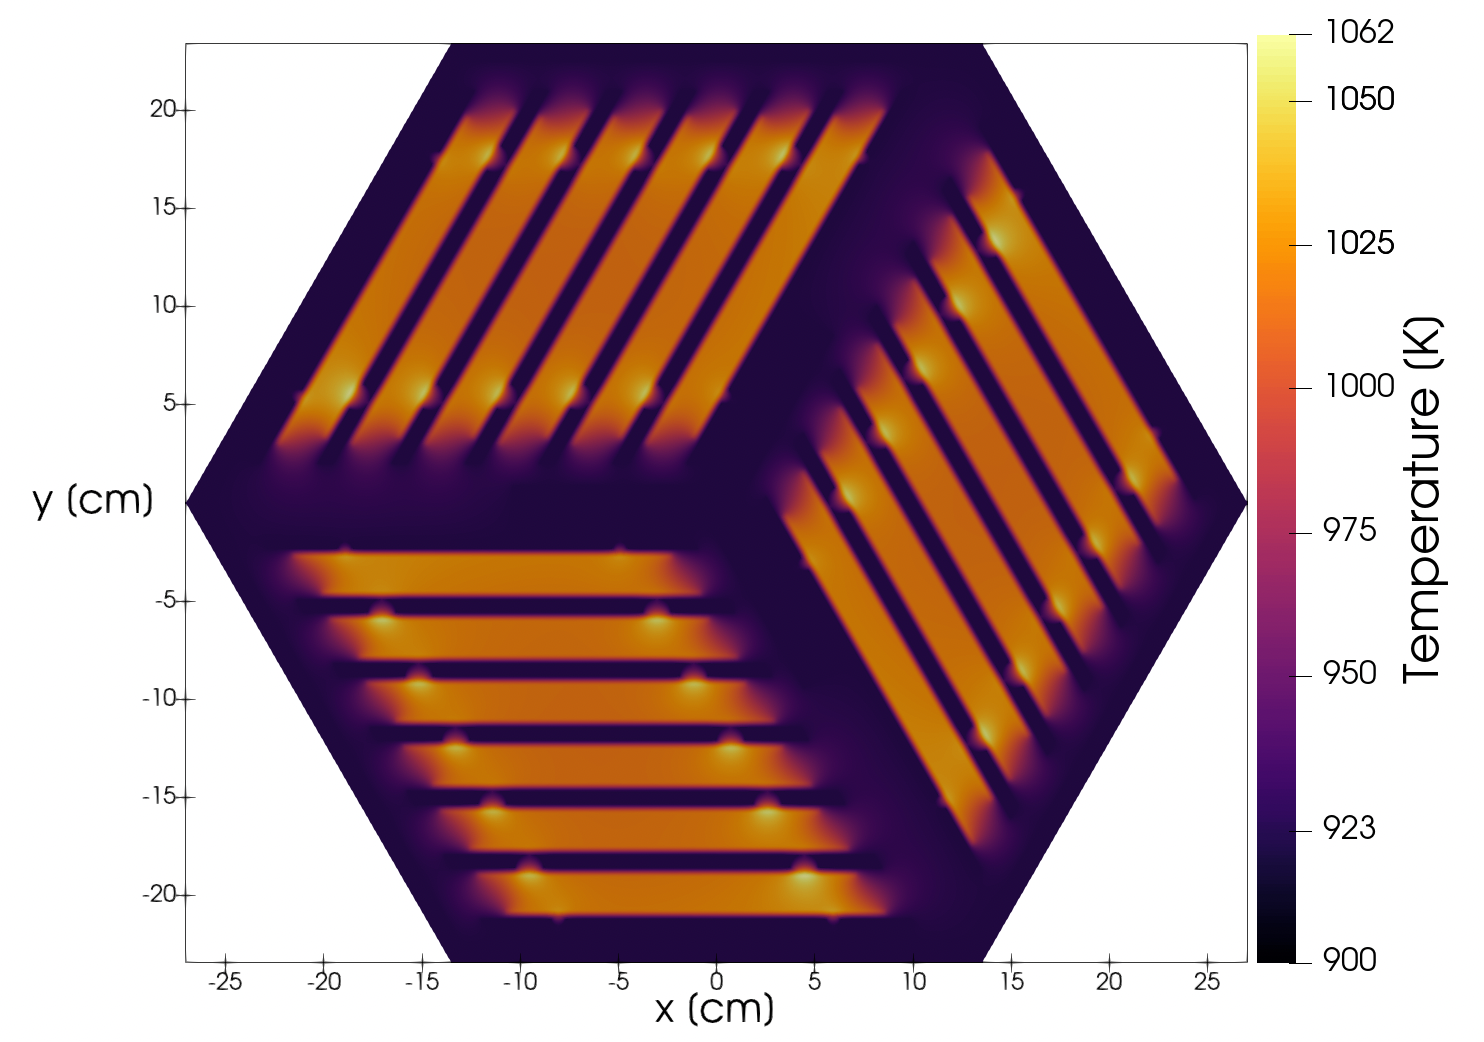
\includegraphics[width=\linewidth]{benchmark-temperature-model.png} 
    \caption{2D temperature distribution in the \acrfull{AHTR} full assembly generated 
    by Moltres.}
    \label{fig:benchmark-temperature-model}
\end{figure}
The average temperature distribution across the fuel planks are similar at approximately 
1025K, while the graphite structure has an average temperature of approximately 935K. 
As defined in the temperature model setup, the \gls{FLiBe} coolant channel 
(inter-plank, inter-assembly, control rod slot) regions remain at 923K.
The temperature peaks at 1062K, which occur in the fuel stripes near the spacers. 
This could be due to the extra moderation provided by the graphite spacers.
This highlights the significance of the spacers' material composition and location in 
causing higher temperature peaks. 

\pagebreak
\section{Summary}
\glsresetall
This chapter described the \gls{FHR} benchmark specifications, \gls{AHTR} design,
Phase I-A and I-B results obtained by the \gls{UIUC} team, and the \gls{FHR} 
temperature model's results.  
The benchmark results highlight the \gls{AHTR}'s passive safety behavior with 
negative temperature coefficients. 
Results such as a lower $k_{eff}$ for the \gls{AHTR} configuration with 
higher heavy metal loading demonstrated that increased fuel packing does not always 
correspond with increased $k_{eff}$ due to self-shielding effects.
These results hint at the possibility of minimizing fuel required by optimizing 
for heterogenous fuel distributions within the core. 
This will be further explored in the later chapters. 
The temperature model demonstrates that the \gls{AHTR}'s temperature peaks are in the 
fuel stripes near the spacers, highlighting to reactor designers that 
spacer material and location in the \gls{AHTR} geometry impact temperature peaks. 

%\include(fhr-multiphysics)
%\chapter{ROLLO: Reactor evOLutionary aLgorithm Optimizer}
\label{chap:rollo}
% todo: need a nice rollo v1.0 citation
In this chapter, I introduce the \gls{ROLLO} framework developed for this dissertation. 
\gls{ROLLO} is a Python package that applies evolutionary algorithm 
techniques to optimize nuclear reactor design. 
Applying evolutionary algorithms to nuclear design problems is not new, as
discussed in Section \ref{sec:opt}. 
Reactor designers have individually customized available evolutionary algorithm 
packages for their reactor design optimization problems.
However, the evolutionary algorithm setup is highly customizable with
an assortment of genetic algorithm designs and related operators.
A reactor designer unfamiliar with evolutionary algorithms will have
to go through the cumbersome process of customizing a genetic algorithm 
for their needs and determine which operators and hyperparameters work best for 
their problem. 
Furthermore, computing fitness values with nuclear software is computationally 
expensive, necessitating using supercomputers. 
Reactor designers have to set up parallelization to use the genetic algorithm 
in concert with nuclear software.

Therefore, the motivation for \gls{ROLLO} is to limit these inconveniences and 
facilitate using evolutionary algorithms for reactor design optimization.
\gls{ROLLO} provides a general genetic algorithm framework, sets up 
parallelization for the user, and promotes usability with an input file 
that only exposes mandatory parameters.
\gls{ROLLO} strives to be effective, flexible, open-source, parallel, reproducible, 
and usable. 
I briefly summarize how \gls{ROLLO} achieves these goals:
\begin{itemize}
    \item Effective: \gls{ROLLO} is well documented and tested.
    \item Flexible: This dissertation uses \gls{ROLLO} to 
    explore arbitrary reactor geometries and heterogeneous fuel distributions. 
    However, future users might want to utilize \gls{ROLLO} 
    to explore other arbitrary design parameters. Thus, I designed the \gls{ROLLO}
    framework accordingly. The user can vary any imaginable parameter 
    because \gls{ROLLO} uses a templating method to edit the input file of the 
    coupled software.
    \item Open-source: \gls{ROLLO} is open-source and version-controlled on Github 
    \cite{chee_rollo_2021}, benefitting from the innovation of the open-source 
    community. \gls{ROLLO} also utilizes the well-documented, open-source 
    \gls{DEAP} \cite{fortin_deap_2012} Python package to drive the evolutionary 
    algorithm optimization process.
    \item Parallel: Users have the option to run \gls{ROLLO} in parallel so that 
    they may effectively use the computational resources available. 
    \item Reproducible: Data from every \gls{ROLLO} run saves into a unique, pickled 
    checkpoint file (pickle is a Python module that serializes Python objects). 
    The checkpoint file contains the \gls{ROLLO} input file and coupled evaluator's 
    scripts enabling results replication. The checkpoint file also acts as a restart 
    file for partially completed simulations. 
\end{itemize}

\gls{ROLLO} provides a framework to couple an evolutionary algorithm driver with nuclear 
software, such as neutron transport and thermal-hydraulics codes. 
\gls{ROLLO} is nuclear code-agnostic and does not have any hard dependencies on any 
nuclear software. 
Figure \ref{fig:genetic_alg} from Chapter \ref{chap:lit-review} outlined a
general evolutionary algorithm iterative problem solving process. 
I modified Figure \ref{fig:genetic_alg} to produce Figure 
\ref{fig:genetic_alg_nuclear}, which depicts how the nuclear transport and 
thermal-hydraulics software fit within \gls{ROLLO}'s evolutionary algorithm 
optimization process. 
% need to update with new algorithm style
\begin{figure}[htbp]
    \centering
    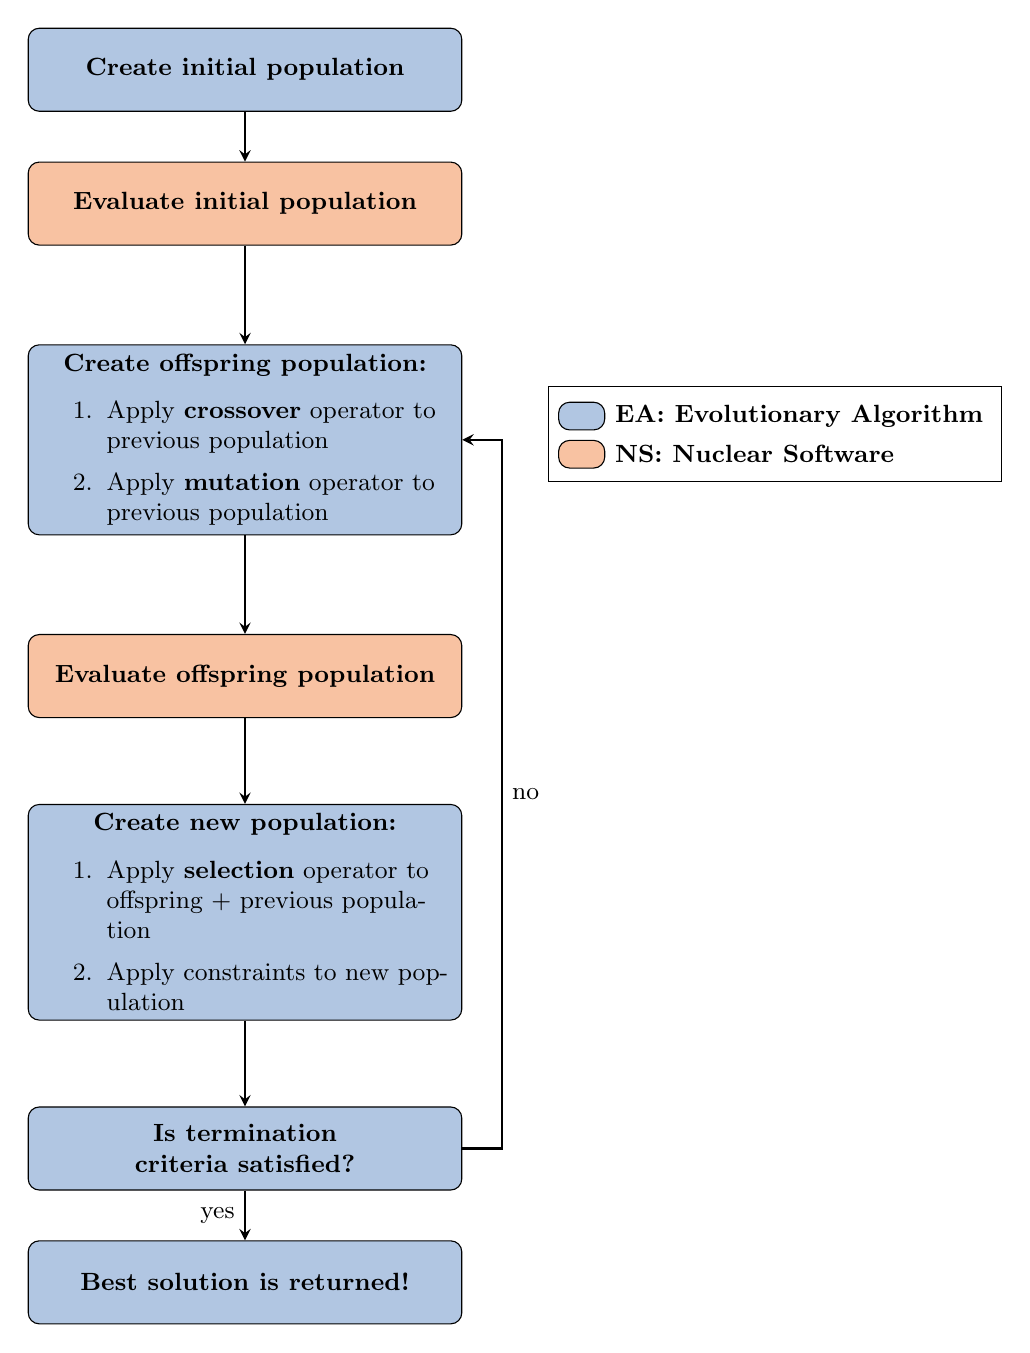
\begin{tikzpicture}[node distance=1.7cm]
            \tikzstyle{every node}=[font=\small]
            \node (1) [lbblock] {\textbf{Create initial population}};
            \node (2) [loblock, below of=1] {\textbf{Evaluate initial population}};
            \node (3) [lbblock, below of=2, yshift = -1.3cm] {\textbf{Create offspring population:} \\ 
            \begin{enumerate} \item Apply \textbf{crossover} operator to previous population
                              \item Apply \textbf{mutation} operator to previous population
                              \end{enumerate}};
            \node (4) [loblock, below of=3, yshift=-1.3cm] {\textbf{Evaluate offspring population}};
            \node (7) [lbblock, below of=4, yshift = -1.3cm] {\textbf{Create new population:} \\
            \begin{enumerate} \item Apply \textbf{selection} operator to offspring + previous population
                              \item Apply constraints to new population
                              \end{enumerate}};
            \node (5) [lbblock, below of=7, yshift=-1.3cm] {\textbf{Is termination \\ criteria satisfied?}};
            \node (6) [lbblock, below of=5] {\textbf{Best solution is returned!}};
            \draw [arrow] (1) -- (2);
            \draw [arrow] (2) -- (3);
            \draw [arrow] (3) -- (4);
            \draw [arrow] (4) -- (7);
            \draw [arrow] (7) -- (5);
            \draw [arrow] (5) -- node[anchor=east] {yes} (6);
            \draw [arrow] (5) -- ([shift={(0.5cm,0cm)}]5.east)-- node[anchor=west] {no} ([shift={(0.5cm,0cm)}]3.east)--(3);
            \matrix [draw,above right,yshift=10.7cm, xshift=0cm] at (current bounding box.south east) {
            \node [bbblock,label=right:\textbf{EA: Evolutionary Algorithm}] {}; \\
            \node [boblock,label=right:\textbf{NS: Nuclear Software}] {}; \\
            };
    \end{tikzpicture}
    \caption{Process of finding optimal solutions for a problem with a 
    genetic algorithm. Nuclear software evaluates each new population.}
    \label{fig:genetic_alg_nuclear}
\end{figure}
\gls{ROLLO} initially reads and validates the JSON input 
file, initializes the \gls{DEAP} \cite{fortin_deap_2012} genetic algorithm 
hyperparameters and operators, and finally runs the genetic algorithm following 
the flow chart in Figure \ref{fig:genetic_alg_nuclear}, in which the nuclear 
software evaluates each individual reactor model's fitness. 

The subsequent sections describe \gls{ROLLO}'s evolutionary algorithm driver 
software \gls{DEAP} (Section \ref{sec:rollo-ea}), input file structure (Section 
\ref{sec:rollo-input-file}), software architecture (Section \ref{sec:rollo-archi}), 
verification studies (Section \ref{sec:rollo-verification}), and convergence criteria
(Section \ref{sec:rollo-convergence}). 
Appendix B lists all the data and analysis related to this chapter to enable the 
reproduction of all the simulations.

\section{Evolutionary Algorithm Driver}
\label{sec:rollo-ea}
Evolutionary algorithm computation uses sophisticated, diverse techniques 
and mechanisms, resulting in even the most well-designed software frameworks 
being complicated under the hood. 
Utilizing an existing evolutionary algorithm framework presents implementation 
challenges as the user must edit the framework's source code to customize it for their 
application and hyperparameters \cite{fortin_deap_2012}. 
Therefore, a computation framework that gives the user the capability to build 
custom evolutionary algorithms is ideal for this project.

Many evolutionary algorithm computation packages exist: 
\gls{DEAP} \cite{fortin_deap_2012}, Pymoo \cite{blank_pymoo_2020}, inspyred 
\cite{garrett_inspyred_2014}, Pyevolve \cite{perone_pyevolve_2009}, and 
OpenBEAGLE \cite{gagne_open_2002}.
\gls{DEAP} is the newest package and places a high value on code 
compactness and clarity \cite{fortin_deap_2012}. 
\gls{DEAP} is the only framework that allows the user to prototype evolutionary 
algorithms rapidly and define custom algorithms without digging deep into 
the source code to modify hyperparameters and their application methods.
Accordingly, I chose \gls{DEAP} to drive the \gls{ROLLO} framework's 
evolutionary algorithm component. 
\gls{DEAP} provides building blocks for each optimizer function and allows the 
user to customize a specialized algorithm to fit their project \cite{fortin_deap_2012}.

\subsection{Distributed Evolutionary Algorithms in Python}
\label{sec:deap-works}
\gls{DEAP} is composed of two structures: a \textit{creator} and a 
\textit{toolbox}.  
The \textit{creator} module allows the run-time creation of classes via 
inheritance and composition, enabling individual and population creation 
from any data structure: lists, sets, dictionaries, trees, etc \cite{fortin_deap_2012}. 
The \textit{toolbox} is a container that the user manually populates.
In the \textit{toolbox}, the user defines the selection, crossover, and 
mutation operator types and their respective hyperparameters.
For example, the user registers a crossover operator under the `mate'
alias and a selection operator under the `select' alias. 
Then, the evolutionary algorithm uses these aliased operators from the 
\textit{toolbox}. 
If the user wants to change the crossover operator, they update the 
`mate' alias in the \textit{toolbox} while keeping the evolutionary algorithm 
unchanged \cite{fortin_deap_2012}. 

Figure \ref{fig:deap-code} illustrates \gls{DEAP}'s usage of the \textit{creator} and
\textit{toolbox} modules. 
\begin{figure}[htbp]
    \begin{minted}[
        frame=lines,
        framesep=2mm,
        baselinestretch=1.2,
        fontsize=\footnotesize,
        linenos
        ]{python}
        
        from deap import creator, base, tools, algorithms
        creator.create("Objective", base.Fitness, weights=(-1.0,)) # minimum
        creator.create("Individual", list, fitness=creator.Objective)

        toolbox = base.Toolbox()
        toolbox.register("variable_1", random.uniform, 0.0, 10.0)
        toolbox.register("variable_2", random.uniform, -1.0, 0.0)
        def individual_creator():
            return creator.Individual([toolbox.variable_1(), toolbox.variable_2()])
        toolbox.register("individual", individual_creator())
        toolbox.register("population", tools.initRepeat, list, toolbox.individual)
        def evaluator_fn(individual):
            return tuple([sum(individual)])
        toolbox.register("evaluate", evaluator_fn)
        toolbox.register("select", tools.selBest, k=5)
        toolbox.register("mutate", tools.mutPolynomialBounded, eta=0.5, low=[0, -1], up=[-1, 0])
        toolbox.register("mate", tools.cxOnePoint)
    \end{minted}
    \caption{DEAP sample code demonstrating the usage of the \textit{creator} and
    \textit{toolbox} modules to initialize the genetic algorithm. In \gls{ROLLO}, \gls{DEAP}'s 
    \textit{creator} and \textit{toolbox} modules are initialized in the source 
    code based on the genetic algorithm parameters defined by the user in the 
    \gls{ROLLO} input file. }
    \label{fig:deap-code}
\end{figure}
Line 2 creates a single-objective fitness class, \texttt{Objective}. 
The first argument defines the derived class's name; the second argument 
specifies the inherited base class, \texttt{base.fitness}; the third 
argument indicates the objective fitness ($-1.0$ indicates a minimum objective, 
$+1.0$ indicates a maximum objective). 
Line 3 derives an \texttt{Individual} class from the standard Python list type
and defines its fitness attribute as the newly created \texttt{Objective} object. 
Lines 5-9 initialize the \gls{DEAP} toolbox, register 
\texttt{variable\_1} and \texttt{variable\_2} with their upper and lower bounds, 
and defines the \texttt{individual\_creator} function to return an 
\texttt{Individual} initialized with \texttt{variable\_1} and \texttt{variable\_2}. 
Lines 10-11 and 14-17 are aliases for initializing individuals and populations, 
specifying variation operators (\texttt{select}, \texttt{mutate}, \texttt{mate}), 
and evaluating individual fitness (\texttt{evaluate}) \cite{fortin_deap_2012}. 
Lines 12-13 define the evaluation function that returns the fitness values. 

\gls{ROLLO} initializes \gls{DEAP}'s \textit{creator} and \textit{toolbox} modules 
based on the genetic algorithm parameters defined by the user in the \gls{ROLLO} 
input file. 
The evaluation function runs the nuclear software and returns user-defined 
fitness values. 

\subsection{ROLLO Evolutionary Algorithm Implementation}
\gls{DEAP} creators provided variations of a classical genetic algorithm 
exposing different explicitness levels \cite{fortin_deap_2012}. 
The high-level examples use the built-in \gls{DEAP} genetic algorithms, 
whereas the low-level example completely unpacks the genetic algorithm to expose 
a generational loop. 
I included an unpacked genetic algorithm in ROLLO's 
\textbf{\textit{Algorithm}} class, depicted in Figure \ref{fig:genetic_alg_nuclear}. 
The algorithm begins by initializing the starting population and evaluating 
each individual's fitness value. 
Then, it enters a generational loop. 
During each iteration, the mating and mutation operators are applied to the population
to create an offspring population, and all offspring individuals are evaluated. 
The selection operator is then applied to both the previous and offspring populations 
to select the best individuals to create the new population. 
Finally, the constraints are applied, and the results are saved.
Applying the selection operator to the combined previous and offspring 
populations expands the population, ensuring the effectiveness of 
elitism selection operators, such as NSGA-II, which work well 
for multiobjective optimization. 

\section{ROLLO Input File}
\label{sec:rollo-input-file}
\gls{ROLLO}'s input file is in JSON format. 
There are four sections that the user must define: \\ \texttt{control\_variables}, 
\texttt{evaluators}, \texttt{constraints}, and \texttt{algorithm}. 
Figure \ref{fig:rollo-input} shows an example \gls{ROLLO} input file. 
In this example, \gls{ROLLO} uses a genetic algorithm with user-defined 
hyperparameters, defined in the \texttt{algorithm} secion, to minimize the 
\texttt{output1} parameter.
The OpenMC evaluator accepts input parameters: \texttt{variable1} and 
\texttt{variable2}, and calculates the \texttt{output1} parameter.
\begin{figure}[htbp]
    \begin{minted}[
        frame=lines,
        framesep=2mm,
        baselinestretch=1.2,
        fontsize=\footnotesize,
        linenos
        ]{json}
        {
            "control_variables": {
                "variable1": {"min": 0.0, "max": 10.0}, 
                "variable2": {"min": -1.0, "max": 0.0}
            }, 
            "evaluators": {
                "openmc": {
                    "order": 0,
                    "inputs": ["variable1", "variable2"],
                    "input_script": ["python", "openmc_inp.py"],
                    "execute": [["openmc"],],
                    "outputs": ["output1", "output2"]
                    "output_script": ["python", "openmc_output.py"], 
                }
            }, 
            "constraints": {
                "output1": {"operator": [">=", "<"], "constrained_val": [1.0, 1.5]}
            }, 
            "algorithm": {
                "objective": ["min"], 
                "weight": [1.0],
                "optimized_variable": ["output1"], 
                "pop_size": 100, 
                "generations": 10, 
                "parallel": "job_control",
                "keep_files": "all",
                "mutation_probability": 0.23,
                "mating_probability": 0.46,
                "selection_operator": {"operator": "selTournament", "tournsize":5},
                "mutation_operator": {
                    "operator": "mutPolynomialBounded",
                    "indpb": 0.23,
                    "eta": 0.23
                },
                "mating_operator": {"operator": "cxBlend", "alpha": 0.46}
            }
        }
    \end{minted}
    \caption{\acrfull{ROLLO} sample JSON input file.}
    \label{fig:rollo-input}
\end{figure}
Next, I describe how to define each section of a \gls{ROLLO} input file. 
The \gls{ROLLO} documentation \cite{chee_documentation_2021} provides further 
descriptions for setting up a \gls{ROLLO} input file.

\subsection{Control Variables}
I use the term control variables to refer to parameters the genetic algorithm will 
vary (conventionally, a control variable is held constant in a research study 
however this is not the case for \gls{ROLLO}).
The user must specify the minimum and maximum values for each control variable.
For example, Lines 2 to 5 in Figure \ref{fig:rollo-input} demonstrate that the 
control variables, \texttt{variable1} and \texttt{variable2}, 
will be varied from 0 to 10 and -1 to 0, respectively. 
For example, in traditional reactor design, a control variable might be fuel 
enrichment. 

\subsection{Evaluators}
Evaluators are the nuclear software \gls{ROLLO} utilizes to calculate objective functions. 
\gls{ROLLO} is nuclear code-agnostic and does not have hard dependencies on any 
nuclear software.
Thus, it is up to the user to ensure that the nuclear software and their corresponding 
executables are correctly installed. 
In a single \gls{ROLLO} input file, users may define any number of evaluators. 
For each evaluator, mandatory parameters are \texttt{order}, \texttt{input\_script}, 
\texttt{inputs}, and \texttt{outputs}, and the optional parameters are
\texttt{execute} and \texttt{output\_script}. 
Table \ref{tab:evaluator-inputs} describes each evaluator's mandatory and optional parameters 
in the \gls{ROLLO} \texttt{evaluators}' input file section.  
\begin{table}[htbp]
    \centering
    \onehalfspacing
    \caption{\acrfull{ROLLO} \texttt{evaluator}: Input Parameter Descriptions.}
	\label{tab:evaluator-inputs}
    \footnotesize
    \begin{tabular}{l|lp{2.5cm}p{7cm}}
    \hline
    & \textbf{Parameter} & \textbf{Type} & \textbf{Description} \\
    \hline
    \multirow{9}{2cm}{Mandatory Parameters} & \texttt{order} & int 
    & evaluator's operational order compared to other evaluators (indexed by 0) \\
    \cline{2-4}
    & \texttt{inputs} & list of strings & control variables to be placed in the input 
    script template \\
    \cline{2-4}
    & \texttt{input\_script} & list of strings (2-element) & 1st element: executable to 
    run input script, 2nd element: input script template \\
    \cline{2-4}
    & \texttt{outputs} & list of strings & output variables that the evaluator will return to the genetic algorithm \\
    \hline
    \multirow{4}{2cm}{Optional Parameters} & \texttt{execute} & list of 2-element lists &
    enables users to run other executables or files beyond the input and output scripts. 
    1st element: executable to run file, 2nd element: file to run \\
    \cline{2-4}
    & \texttt{output\_script} & list of strings (2-element) & 1st element: executable to 
    run output script, 2nd element: output script template \\
    \hline 
    \end{tabular}
    \end{table}

\gls{ROLLO} utilizes jinja2 templating \cite{ronacher_welcome_2018} to insert 
the control variable values into the \texttt{input\_script}.
Users must include each evaluator's input file template in the same directory as the \gls{ROLLO} input 
file. 
Users must also ensure the template variables correspond to the \texttt{inputs} defined in the 
corresponding evaluator's section in the ROLLO input file. 
Lines 6 to 13 in the \gls{ROLLO} input file (Figure \ref{fig:rollo-input}) demonstrate 
that \texttt{variable1} and \texttt{variable2} are \texttt{inputs} into the 
\texttt{openmc\_inp.py} \texttt{input\_script}. 
Figure \ref{fig:openmcinp.py} shows the template and templated openmc script; 
once the \texttt{openmc\_inp.py} \texttt{input\_script} is templated, 
\texttt{\{\{variable1\}\}} and \texttt{\{\{variable2\}\}}  on Lines 3 and 4 will be 
replaced with values selected by the \gls{ROLLO} genetic algorithm. 
\begin{figure}[htbp]
    \begin{minipage}{0.4\textwidth}
        \centering
    \begin{minted}[
        frame=lines,
        framesep=2mm,
        baselinestretch=1.2,
        fontsize=\footnotesize,
        linenos
        ]{python}
        import openmc 
        # templating 
        variable1 = {{variable1}}
        variable2 = {{variable2}}
        # run openmc 
        ... 
    \end{minted}
    \end{minipage}
    \hspace{2cm}
    \begin{minipage}{0.4\textwidth}
        \centering
        \begin{minted}[
            frame=lines,
            framesep=2mm,
            baselinestretch=1.2,
            fontsize=\footnotesize,
            linenos
            ]{python}
            import openmc 
            # templating 
            variable1 = 3.212
            variable2 = -0.765
            # run openmc 
            ... 
        \end{minted}
        \end{minipage}
    \caption{\texttt{openmc\_inp.py} input script template (left). 
             Templated \texttt{openmc\_inp.py} with variable1 and variable2 
             values defined (right).}
    \label{fig:openmcinp.py}
\end{figure}

\gls{ROLLO} uses two methods to return an output variable to the genetic algorithm. 
First, \gls{ROLLO} will automatically return the input parameter's value if the output 
parameter is also an input parameter. 
Second, the user may include an \texttt{output\_script} that returns the desired 
output parameter. 
The \texttt{output\_script} must include a line that prints a dictionary containing 
the output parameters' names and their corresponding value as key-value pairs. 

\subsection{Constraints}
In the constraints section, the user can define constraints on any output parameter. 
Any individual that does not meet the defined constraints is removed from the 
population, encouraging the proliferation of individuals that meet the 
constraints. 
For each constrained output parameter, the user lists the \texttt{operator}s 
and \texttt{constrained\_val}s as in Line 17 of the \gls{ROLLO} input file 
(Figure \ref{fig:rollo-input}). 
Thus, for this \gls{ROLLO} simulation, \texttt{output\_1} is constrained to be 
$>= 1.0$ and $< 1.5$. 
For example, for reactor safety, a constraint might be the maximum temperature in the 
core.

\subsection{Algorithm}
In the algorithm section, users define the simulation's general settings and the
genetic algorithm's hyperparameters. 
The mandatory input parameters include \texttt{optimized\_variable}, \texttt{objective},
\texttt{pop\_size}, and \texttt{generations}.
The optional input parameters include \texttt{parallel}, \texttt{keep\_files}, \\
\texttt{mutation\_probability}, \texttt{mating\_probability}, 
\texttt{selection\_operator}, \texttt{mutation\_operator}, 
and \texttt{mating\_operator}. 
Lines 17 to 31 in the example \gls{ROLLO} input file (Figure \ref{fig:rollo-input}) 
demonstrate \texttt{algorithm} specifications. 
Table \ref{tab:algorithm-inputs} describes these input parameters in detail. 
\begin{table}[htbp]
    \centering
    \onehalfspacing
    \caption{\acrfull{ROLLO} \texttt{algorithm}: Input Parameter Descriptions.}
	\label{tab:algorithm-inputs}
    \scriptsize
    \begin{tabular}{l|lp{1.5cm}p{3.7cm}p{3.5cm}}
    \hline
    & \textbf{Parameter} & \textbf{Type} & \textbf{Description} & \textbf{Default} \\
    \hline
    \multirow{9}{1.8cm}{Mandatory Parameters} 
    & \texttt{optimized\_variable} & list of strings & variables to be optimized & -\\
    \cline{2-5}
    & \texttt{objective} & list of strings & options include: min or max,
    each objective corresponds to a variable in \texttt{optimized\_variable} & -\\
    \cline{2-5}
    & \texttt{pop\_size} & int & population size & -\\
    \cline{2-5}
    & \texttt{generations} & int & number of generations & -\\
    \hline
    \multirow{15}{1.8cm}{Optional Parameters} 
    & \texttt{parallel} & string & options include: \textit{none}, \textit{multiprocessing}, \textit{job\_control} & \textit{none} \\
    \cline{2-5}
    & \texttt{keep\_files} & string & options include: \textit{none}, \textit{only\_final}, \textit{all} & \textit{none} \\
    \cline{2-5}
    & \texttt{mutation\_probability} & float & mutation probability & 0.23 \\
    \cline{2-5}
    & \texttt{mating\_probability} & float & mating probability & 0.47 \\
    \cline{2-5}
    & \texttt{selection\_operator} & dict & see Table \ref{tab:deap_operators} & \scriptsize{{"operator": "selTournament", "tournsize": 5}}\\
    \cline{2-5}
    & \texttt{mutation\_operator} & dict & see Table \ref{tab:deap_operators} & \scriptsize{{"operator": "mutPolynomialBounded", "eta": 0.23, "indpb": 0.23}}\\
    \cline{2-5}
    & \texttt{mating\_operator} & dict & see Table \ref{tab:deap_operators} & \scriptsize{{"operator": "cxBlend", "alpha": 0.46}}\\
    \hline 
    \end{tabular}
    \end{table}
The hyperparameter default values are selected based on hyperparameter studies conducted 
for a single objective \gls{FHR} optimization. 
Section \ref{sec:hyperparameter-studies} describes the hyperparameter studies. 

As mentioned previously in Section \ref{sec:genetic_alg}, it is important to 
select genetic algorithm hyperparameters that balance the extent of exploration 
and exploitation.
% todo: add this phrasing earlier in chapter too. 
For each operator, users choose from a list of operators and define each
of their required hyperparameters. 
Table \ref{tab:deap_operators} shows the available operators and their respective 
hyperparameters. 
Descriptions for each operator can be found in Section \ref{sec:genetic_alg}.
\begin{table}[htbp]
    \centering
    \onehalfspacing
    \caption{Selection, mutation, and mating operators available in 
    \acrfull{ROLLO} and their corresponding hyperparameters. n/a indicates that 
    the operator does not have associated hyperparameters. }
	\label{tab:deap_operators}
    \footnotesize
    \begin{tabular}{l|p{0.23\textwidth}|p{0.55\textwidth}}
    \hline
    \textbf{Operator} & \textbf{Available Options} & \textbf{Hyperparameters} \\ \hline
    \multirow{4}{1cm}{Selection} & \texttt{selTournament} & \texttt{tournsize}: no. of individuals in each tournament\\ \cline{2-3}
    & \texttt{selNSGA2} & n/a \\ \cline{2-3}
    & \texttt{selBest} & n/a \\ \hline
    \multirow{2}{1cm}{Mutation} & \multirow{2}{2cm}{\texttt{mutPolynomialBounded}} & \texttt{eta}: crowding degree of the mutation\\  
    && \texttt{indpb}: independent probability for each attribute to be mutated\\ \hline
    \multirow{3}{1cm}{Mating} & \texttt{cxOnePoint} & n/a \\ \cline{2-3}
    & \texttt{cxUniform} & \texttt{indpb}: independent probability for each attribute to be exchanged\\ \cline{2-3}
    & \texttt{cxBlend} & \texttt{alpha}: Extent of the interval that the new values can be drawn for each attribute on both sides of the parents’ attributes\\ \hline
    \end{tabular}
    \end{table}

\section{ROLLO Software Architecture}
\label{sec:rollo-archi}
This section describes the \gls{ROLLO} v1.0 software architecture and 
how each part contributes the reactor design optimization process.
Table \ref{tab:rollo-architecture} outlines the classes in the \gls{ROLLO} software 
and describes each class's purpose.
\begin{table}[htbp]
    \centering
    \onehalfspacing
    \caption{Classes that comprise the \gls{ROLLO} architecture. }
	\label{tab:rollo-architecture}
    \footnotesize
    \begin{tabular}{l|p{0.73\textwidth}}
    \hline
    \textbf{Class} & \textbf{Description} \\ \hline
    \textbf{\textit{InputValidation}} & The \textbf{\textit{InputValidation}} class contains methods 
    to read and validate the JSON \gls{ROLLO} input file to 
    ensure the user defined all key parameters. If they did not, \gls{ROLLO} 
    raises an exception to tell the user which parameters are missing. \\
    \hline
    \textbf{\textit{Evaluation}} & \gls{DEAP}'s fitness evaluator (as mentioned in Section 
    \ref{sec:deap-works}) requires an evaluation function to evaluate each 
    individual's fitness values. 
    The \textbf{\textit{Evaluation}} class contains a method that creates an evaluation 
    function that runs the nuclear software and returns the required fitness values
    defined in the input file. \\
    \hline 
    \textbf{\textit{ToolboxGenerator}} & The \textbf{\textit{ToolboxGenerator}} class initializes
    \gls{DEAP}'s \textit{toolbox} and \textit{creator} modules with genetic algorithm 
    hyperparameters defined in the input file.\\
    \hline
    \textbf{\textit{Constraints}} & The \textbf{\textit{Constraints}} class 
    contains methods to initialize constraints defined in the input file 
    and applies the constraints by removing individuals that do not meet the 
    constraint.\\
    \hline 
    \textbf{\textit{BackEnd}} & The \textbf{\textit{BackEnd}} class contains methods to save 
    genetic algorithm population results into a pickled checkpoint file and to 
    restart a partially completed genetic algorithm from the checkpoint file. \\
    \hline
    \textbf{\textit{Algorithm}} & The \textbf{\textit{Algorithm}} class contains methods to 
    initialize and execute the genetic algorithm. It executes a general genetic 
    algorithm framework that uses the hyperparameters defined in the 
    \textbf{\textit{ToolboxGenerator}}, applies constraints defined in
    \textbf{\textit{Constraints}}, evaluates fitness values using the evaluation 
    function produced by \textbf{\textit{Evaluation}}, and saves all the results 
    with \textbf{\textit{BackEnd}}. \\
    \hline
    \textbf{\textit{Executor}} & The \textbf{\textit{Executor}} class drives the \gls{ROLLO} code
    execution with the following steps: \\
    & 1) User input file validation with \textbf{\textit{InputValidation}} \\
    & 2) Evaluation function generation with \textbf{\textit{Evaluation}} \\
    & 3) \gls{DEAP} toolbox initialization with \textbf{\textit{ToolboxGenerator}} \\ 
    & 4) Constraint initialization with \textbf{\textit{Constraints}} \\ 
    & 5) Genetic algorithm execution with \textbf{\textit{Algorithm}} \\
    \hline
    \end{tabular}
    \end{table}
Figure \ref{fig:rollo_archi} depicts the \gls{ROLLO} software architecture. 
\begin{figure}[htbp]
    \centering
    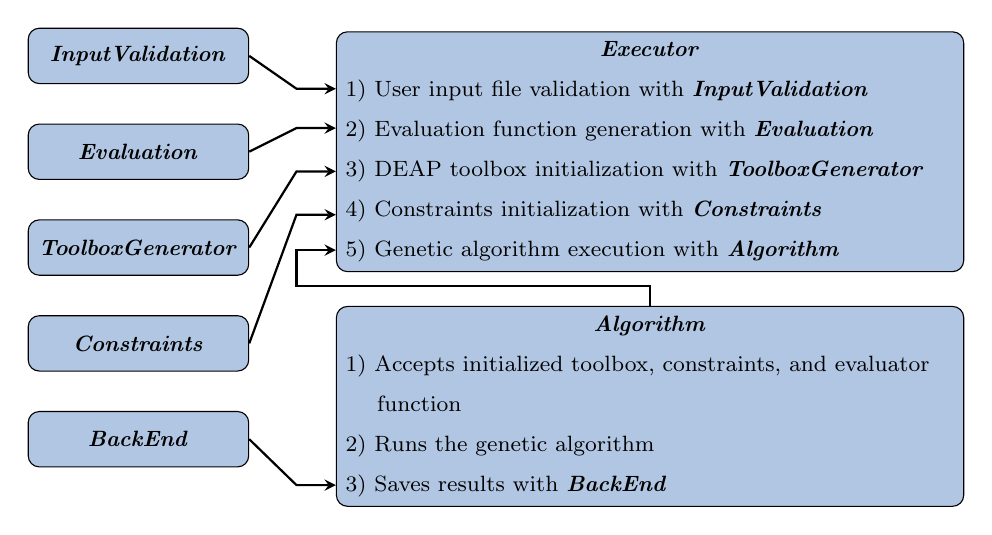
\begin{tikzpicture}[node distance=0.5cm]
        \tikzstyle{every node}=[font=\footnotesize]
        \node (1) [b72block] {\textbf{\textit{InputValidation}}};
        \node (2) [b72block, below=of 1] {\textbf{\textit{Evaluation}}};
        \node (3) [b72block, below=of 2] {\textbf{\textit{ToolboxGenerator}}};
        \node (4) [b72block, below=of 3] {\textbf{\textit{Constraints}}};
        \node (5) [b72block, below=of 4] {\textbf{\textit{BackEnd}}};
        \node (6) [b223block, right=of 2, yshift=0cm, xshift=0.6cm] 
        {\baselineskip=14.5pt \textbf{\textit{Executor}} \\ \raggedright 
        1) User input file validation with \textbf{\textit{InputValidation}} \\ 
        2) Evaluation function generation with \textbf{\textit{Evaluation}} \\ 
        3) \gls{DEAP} toolbox initialization with \textbf{\textit{ToolboxGenerator}} \\ 
        4) Constraints initialization with \textbf{\textit{Constraints}} \\ 
        5) Genetic algorithm execution with \textbf{\textit{Algorithm}} \\};
        \draw [arrow] (1) -- ([shift={(0cm,0cm)}]1.east) -- ([shift={(-0.5cm,0.8cm)}]6.west)--([shift={(0cm,0.8cm)}]6.west);
        \draw [arrow] (2) -- ([shift={(0cm,0cm)}]2.east) -- ([shift={(-0.5cm,0.3cm)}]6.west)--([shift={(0cm,0.3cm)}]6.west);
        \draw [arrow] (3) -- ([shift={(0cm,0cm)}]3.east) -- ([shift={(-0.5cm,-0.25cm)}]6.west)--([shift={(0cm,-0.25cm)}]6.west);
        \draw [arrow] (4) -- ([shift={(0cm,0cm)}]4.east) -- ([shift={(-0.5cm,-0.8cm)}]6.west)--([shift={(0cm,-0.8cm)}]6.west);
        \node (7) [b223block, right=of 4, yshift=-0.8cm, xshift=0.6cm] 
        {\baselineskip=14.5pt \textbf{\textit{Algorithm}} \\ \raggedright 
        1) Accepts initialized toolbox, constraints, and evaluator \\ \hspace{0.3cm} function \\
        2) Runs the genetic algorithm \\
        3) Saves results with \textbf{\textit{BackEnd}} \\};
        \draw [arrow] (7) -- ([shift={(0.cm,0.25cm)}]7.north) -| ([shift={(-0.5cm,-1.25cm)}]6.west) -- ([shift={(0cm,-1.25cm)}]6.west);
        \draw [arrow] (5) -- ([shift={(0cm,0cm)}]5.east) -- ([shift={(-0.5cm,-1cm)}]7.west)--([shift={(0cm,-1cm)}]7.west);
    \end{tikzpicture}
    \caption{Visualization of \gls{ROLLO} architecture.}
    \label{fig:rollo_archi}
\end{figure}
When the user runs a \gls{ROLLO} input file, the \textbf{\textit{Executor}} class 
drives \gls{ROLLO}'s execution from beginning to end.
The \textbf{\textit{Executor}} calls \textbf{\textit{InputValidation}} to 
parse the input file to ensure that the user defined all mandatory parameters
and used the correct formatting.
Next, it initializes an \textbf{\textit{Evaluation}} object based on the 
\texttt{evaluators} specifications in the input file. 
It uses the \textbf{\textit{Evaluation}} object to create a function that will 
run each evaluator software with the desired input parameters and return the 
output parameters calculated by the evaluator software. 
Next, it uses the \textbf{\textit{ToolboxGenerator}} to create an initialized 
DEAP toolbox object based on the input file's \texttt{algorithm} specifications. 
The \textbf{\textit{ToolboxGenerator}} object accepts the 
\textbf{\textit{Evaluation}} object and registers it as the toolbox's `evaluate' 
tool.  
Then, it initializes a \textbf{\textit{Constraints}} object to contain 
\texttt{constraints} specified in the input file. 
Next, the \textbf{\textit{Executor}} initializes an \textbf{\textit{Algorithm}} 
object that accepts the initialized \gls{DEAP} toolbox and \textbf{\textit{Constraints}} 
object. 
Finally, the \textbf{\textit{Executor}} class uses a method in the 
\textbf{\textit{Algorithm}} object to run the general genetic algorithm. 
The \textbf{\textit{Executor}} class uses the hyperparameters from the \gls{DEAP} 
toolbox, applies constraints defined in the \textbf{\textit{Constraints}} object, 
and calculates objective functions using the evaluation function created by the 
\textbf{\textit{Evaluation}} object; all the while saving the results using the 
\textbf{\textit{BackEnd}} class. 

In the \gls{ROLLO} Github repository \cite{chee_rollo_2021}, I include a tests 
directory that contains unit tests for all methods in the classes described 
above. % todo: update citation
These tests serve both to document how to use \gls{ROLLO} as well as to ensure 
\gls{ROLLO} has feature stability. 

\subsection{Installing and Running ROLLO}
There are two ways to install \gls{ROLLO}.
First, a user may use a package manager such as \gls{PyPI} to install \gls{ROLLO}: 
\texttt{python -m pip install rollo} \cite{chee_rollo_2021}.
Second, a user can download the \gls{ROLLO} repository \cite{chee_rollo_2021}
from Github and install it from source. 

Users run \gls{ROLLO} from the command line interface. 
A user must first set up the \gls{ROLLO} JSON input file and evaluator 
scripts in a directory. 
When running \gls{ROLLO} from the command line, there is one mandatory argument and 
two optional arguments. 
The mandatory argument is the input file (\texttt{-i}). 
The optional arguments are the checkpoint file (\texttt{-c}) and verbosity 
flag (\texttt{-v}).  
The checkpoint file holds the results from the \gls{ROLLO} simulation. 
The checkpoint file also acts as a restart file. 
If a ROLLO simulation ends prematurely, the checkpoint file can be used to restart 
the simulation from the most recent generation.
The verbosity flag turns on verbose output. 
The structure of a command line input for running \gls{ROLLO} is: 

\noindent
\texttt{python -m rollo -i <input file name> -c <checkpoint file name> -v}

The checkpoint file holds the \gls{ROLLO} simulation results and acts as a restart file.
Thus, if a \gls{ROLLO} simulation ends prematurely, users can use the checkpoint file to 
restart the code from the most recent population and continue the simulation. 

\subsection{ROLLO Parallelization}
\label{sec:rollo_parallel}
% todo: motivate the need for parallelization and why it is necessary. 
\gls{ROLLO} has a serial run mode and two modes for parallelization. 
The serial mode runs each reactor model in each generation serially and utilizes a 
map() function to run the nuclear software for each reactor model.
The map function accepts a function and iterable and returns a map object of the results 
by applying the function to each item of the iterable. 
In \gls{ROLLO}, the \textbf{\textit{Evaluation}} class generates the function 
that accepts the reactor model's control variables and runs the nuclear software;
and the iterable is a list containing the control variables for each reactor model. 
The first parallel mode, \textit{multiprocessing}, replaces the default map function 
with the \texttt{multiprocessing\_on\_dill} map \cite{smallshire_multiprocessing_on_dill_nodate}.
The \texttt{multiprocessing\_on\_dill} map splits the iterable into several chunks 
which it submits to the process pool as separate tasks.
This \textit{multiprocessing} mode is useful for parallelizing runs on a local machine or 
a single node on a computer cluster. 
However, it is unable to parallelize across distributed memory systems.

The second parallel mode, \texttt{job\_control}, uses the Unix system's job control 
features to give users more flexibility with parallelization setup. 
This flexibility enables parallelization across distributed memory systems such as 
clusters and supercomputers. 
The second parallel mode does not use the map() function. 
Like the \textit{multiprocessing} mode, the \texttt{job\_control} mode generates a 
function using the \textbf{\textit{Evaluation}} class that accepts the reactor model's control 
variables and runs the nuclear software. 
\gls{ROLLO} will then generate a combined bash command that launches multiple evaluation 
function calls for the different reactor models by backgrounding each command.
For example, a ROLLO simulation with a population size of 2 has a combined command that
looks like this:
\begin{figure}[H]
    \centering
    \begin{minipage}{0.5\textwidth}
    \begin{minted}[
        frame=lines,
        framesep=2mm,
        fontsize=\footnotesize,
        ]{bash}
        cd 0_0
        aprun -n 2 python program1.py &
        sleep 1 
        cd ../0_1 
        aprun -n 2 python program1.py &
        sleep 1 
        wait
    \end{minted}
    \end{minipage}
    \caption{Example combined bash command generated by \gls{ROLLO}'s parallel mode 
    \texttt{job\_control}. Directories $0\_0$ and $0\_1$ refer to the first generation's first 
    and second reactor model (indexed by 0).}
    \label{fig:job-control-example}
\end{figure}
Users define each command in ROLLO's input file; thus, the \texttt{job\_control} mode enables 
more control over the parallelization settings of each command. 
Many nuclear software, such as OpenMC and MOOSE, use \gls{MPI} or OpenMP to parallelize their runs. 
With control over each command, users can continue to utilize the parallel 
versions of the nuclear software, thus, having two layers of parallelization. 
The first layer is the individual software's parallelization, and the second layer is ROLLO's parallelization. 
For example, running four reactor models using ROLLO across 16 nodes on a cluster and assigning each reactor 
model to run in parallel across four nodes. 
Users can find in-depth details about the parallelization setup in the ROLLO documentation
 \cite{chee_documentation_2021}.

\subsection{ROLLO Results Analysis}
The \textbf{\textit{BackEnd}} class manages results from each \gls{ROLLO} simulation. 
\textbf{\textit{BackEnd}} saves all the results in a checkpoint file which will output 
into the same directory as the input file at the end of the simulation. 
The checkpoint file can be loaded into a Jupyter notebook and organized 
to produce desired plots. 
Users can find examples of \gls{ROLLO} results analysis in the \gls{ROLLO} documentation
\cite{chee_documentation_2021}. 

The evaluation function creates a new directory for each generation and individual, 
where it then stores all the evaluators' templated input files and output files 
associated with that particular run. 
The generation and individual values are indexed by zero. 
For example, the directory containing files associated with the tenth individual in 
the genetic algorithm's third generation will be named: 
\texttt{2\_9}.


\section{ROLLO Verification}
\label{sec:rollo-verification}
I conducted multiple verification studies to verify \gls{ROLLO}'s optimization capabilities: 
commonly used evolutionary algorithm single and multiobjective benchmark problems and 
a nuclear reactor-specific problem. 
They prove that \gls{ROLLO}'s evolutionary algorithm is both correctly implemented 
and suitable for conducting nuclear reactor optimization problems. 

\subsection{Ackley Function}
The Ackley function, shown in Equation \ref{eq:ackley}, is a function with a 
large number of local minima but only one global minimum, thus, commonly used as a 
performance test for single-objective optimization algorithms 
\cite{ackley_connectionist_2012}. 
An effective single-objective optimization algorithm should find the Ackley function's 
global minimum point.  
\begin{align}
    \label{eq:ackley}
    f(x) &= -a \cdot exp \left(-b\sqrt{\frac{1}{d}\Sigma_{i=1}^dx_i^2}\right) - 
    exp \left(\frac{1}{d}\Sigma_{i=1}^d cos(cx_i)\right) + a + exp(1) 
\end{align}
The recommended variable values are $a=20$, $b=0.2$, and $c=2\pi$
\cite{surjanovic_ackley_2013}. 
The Ackley function's global minimum point is $f(0,0) = 0$. 
Figure \ref{fig:ackley} shows the resulting two-variable Ackley function.
\begin{figure}[htbp]
    \centering
    \includegraphics[width=0.8\linewidth]{ackley.png} 
    \caption{Two variable Ackley function. Figure reproduced from \cite{surjanovic_ackley_2013}.}
    \label{fig:ackley}
\end{figure}

I added an integration test to \gls{ROLLO} that checks that a default \gls{ROLLO} 
simulation will find the Ackley function's global minimum point. 
If \gls{ROLLO} performed sub-optimally, it would return one of the Ackley 
function's many local minimums. 

\subsection{Binh and Korn Function}
\label{sec:binhandkorn}
The Binh and Korn function \cite{binh_mobes_1997} is a two-objective function:
\begin{align}
    \mbox{Minimize} &= \begin{cases}
        f_1 (x_1,x_2) &= 4x_1^2+4x_2^2 \\
        f_2 (x_1,x_2) &= (x_1-5)^2 + (x_2-5)^2 
    \end{cases} \\
    \mbox{Such that} &= \begin{cases}
        (x_1-8)^2 + (x_2+3)^2 \geq 7.7 \nonumber \\
        0 \leq x_1 \leq 5, 0 \leq x_2 \leq 3 \nonumber
    \end{cases}
\end{align}
We use it as a performance test for multiobjective optimization.
% todo: why is this a good problem? what makes it a good evaluator. 
Figure \ref{fig:binh_paretofront} shows the Binh and Korn function's Pareto front.
\begin{figure}[htbp]
    \centering
    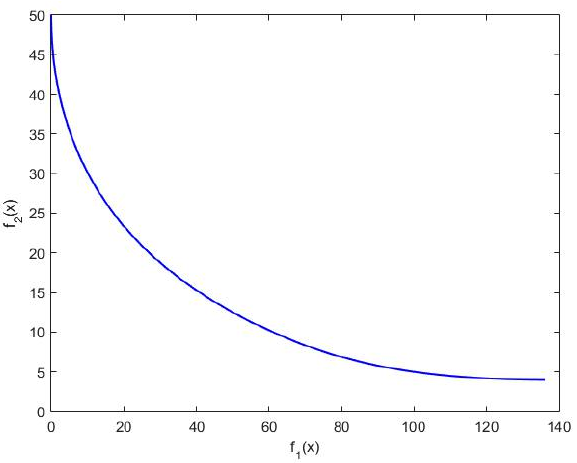
\includegraphics[width=0.7\linewidth]{binh-paretofront.png} 
    \caption{Pareto front of the Binh and Korn test function. Figure reproduced from 
    \cite{bassi_statistics_2018}. }
    \label{fig:binh_paretofront}
\end{figure}
I use the hypervolume indicator to quantify the Pareto front's quality. 
The hypervolume indicator is the most used set-quality indicator for assessing 
stochastic multiobjective optimizers \cite{guerreiro_hypervolume_2020}.
The hypervolume indicator measures the volume (in the objective space) covered by 
non-dominated solutions for problems in which all objectives are to be 
minimized \cite{deb_multi-objective_2001}. 
% todo: remind us of how the reference point is chosen and how it affects hypervolume. 
Figure \ref{fig:pareto_hypervolume} illustrates the hypervolume enclosed by the 
non-dominated solutions (A, B, C, D, E) and reference point, W, in the hatched region 
for a two-dimensional problem.
\begin{figure}[htbp]
    \centering
    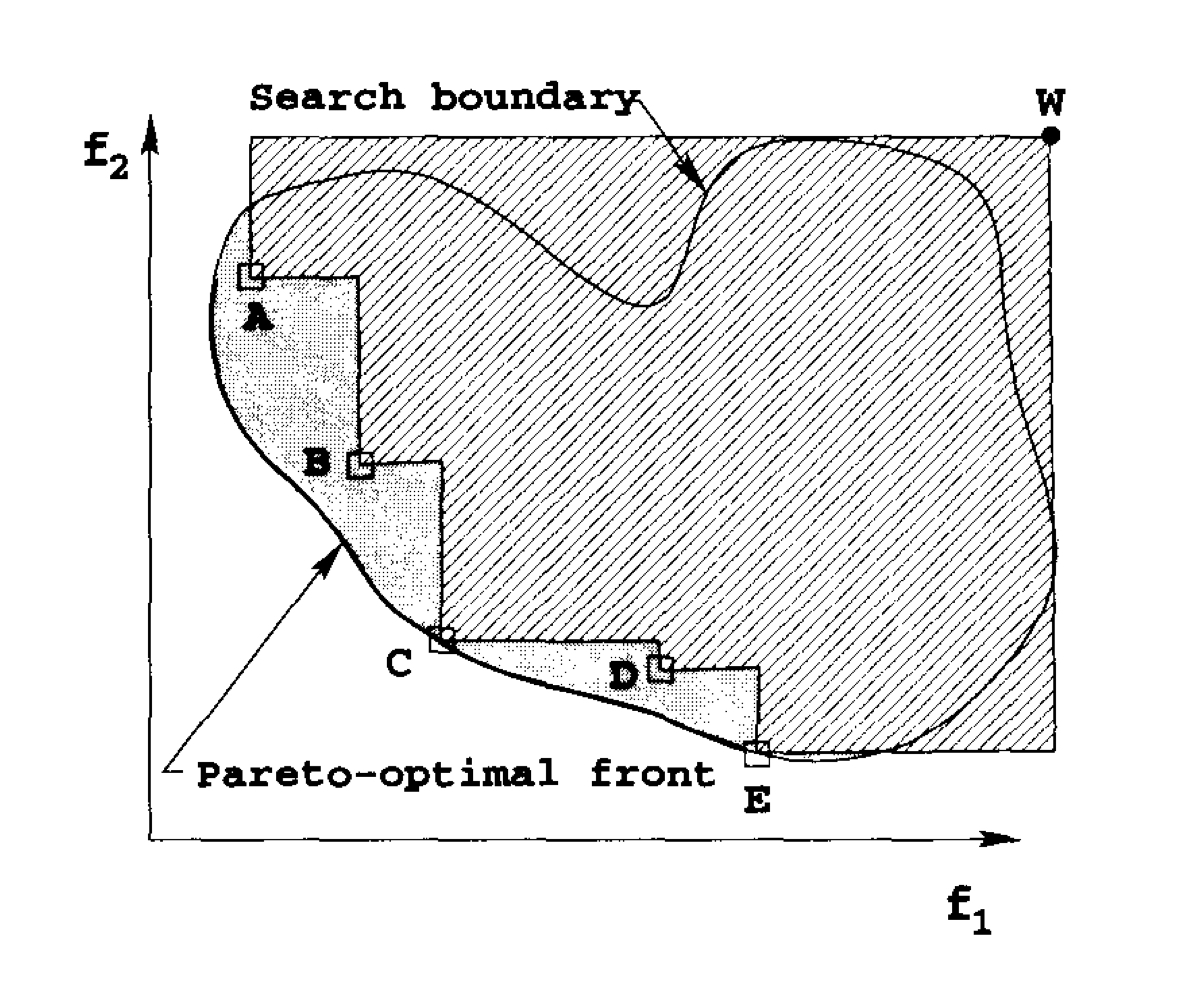
\includegraphics[width=0.7\linewidth]{pareto-hypervolume.png} 
    \caption{Example hypervolume enclosed by non-dominated solutions. Figure reproduced 
    from \cite{deb_multi-objective_2001}. 
    The f1 and f2 axes correspond to the optimization objectives in a \gls{ROLLO} 
    simulation. }
    \label{fig:pareto_hypervolume}
\end{figure}
I added an integration test to ROLLO that checks that a ROLLO simulation will 
find a hypervolume comparable to the ideal Pareto front when minimizing the
Binh and Korn function. 

\subsection{Pu-239 Critical Bare Sphere}
I ran a neutronics verification problem: finding the critical radius for a $^{239}Pu$ 
bare sphere, to ensure successful coupling between \gls{ROLLO} and reactor neutronics 
modeling software, OpenMC \cite{romano_openmc:_2015}. 
The solution to this problem is well studied and readily available in the 
literature \cite{blanchard_updated_1999}. 
Blanchard et al reported that with MCNP4b code and ENDF/B-VI data library, the 
critical mass of a Pu239 bare sphere is 10.00 kg which corresponds to a diameter 
of 9.9cm \cite{blanchard_updated_1999}.
Figure \ref{fig:verification-sphere} shows the ROLLO input file for this verification 
problem. 
In the input file, I vary the radius between 1.0 and 8.0cm, with the objective of 
minimizing the radius while constraining the problem to have $k_{eff} >= 1.0$.
\begin{figure}[htbp]
    \begin{minted}[
        frame=lines,
        framesep=2mm,
        baselinestretch=1.2,
        fontsize=\footnotesize,
        linenos
        ]{json}
        {"control_variables": {
                "radius": {"min": 1.0, "max": 8.0}
            },
            "evaluators": {
                "openmc": {
                    "order": 0,
                    "input_script": ["python", "critical_sphere.py"],
                    "inputs": ["radius"],
                    "outputs": ["keff", "radius"],
                    "output_script": ["python", "get_sphere_keff.py"]
                }
            },
            "constraints": {"keff": {"operator": [">="], 
                            "constrained_val": [1.0]}},
            "algorithm": {
                "parallel": "multiprocessing",
                "keep_files": "none",
                "objective": ["min"],
                "optimized_variable": ["radius"],
                "pop_size": 80,
                "generations": 10
            }}
    \end{minted}
    \caption{\acrfull{ROLLO} JSON input file for finding the minimum radius for 
    a $^{239}Pu$ Critical Bare Sphere.}
    \label{fig:verification-sphere}
\end{figure}
\pagebreak
Figure \ref{fig:critical_sphere.py} shows the OpenMC template used in the 
\gls{ROLLO} simulation. 
\begin{figure}[htbp]
    \begin{minted}[
        frame=lines,
        framesep=2mm,
        baselinestretch=1.2,
        fontsize=\footnotesize,
        linenos
        ]{python}
            import openmc 
            import numpy as np

            pu = openmc.Material()
            pu.set_density("g/cm3", 19.84)
            pu.add_nuclide("Pu239", 1)
            mats = openmc.Materials([pu])
            
            radius = {{radius}}
            
            fuel_sphere = openmc.Sphere(r=radius, boundary_type='vacuum')
            fuel_cell = openmc.Cell(fill=pu, region=-fuel_sphere)
            univ = openmc.Universe(cells=[fuel_cell])
            geom = openmc.Geometry(univ)
            
            settings = openmc.Settings()
            settings.batches = 100
            settings.inactive = 20
            settings.particles = 20000
            settings.temperature = {"multipole": True, "method": "interpolation"}
            
            mats.export_to_xml()
            geom.export_to_xml()
            settings.export_to_xml()
            openmc.run()
    \end{minted}
    \caption{OpenMC template input file used in ROLLO simulation to find the 
    minimum radius for a $^{239}Pu$ Critical Bare Sphere.}
    \label{fig:critical_sphere.py}
\end{figure}  

\gls{ROLLO} successfully finds the critical radius of the $^{239}Pu$ bare sphere 
to be 4.9856cm which corresponds to approximately a 9.9cm diameter. 
The critical sphere's $k_{eff}$ value is 1.00919 $\pm$ 0.00048. 
Figure \ref{fig:verification-radius} and \ref{fig:verification-keff} show the 
radius and $k_{eff}$ evolution through the evolutionary algorithm's 
generations. 
They demonstrate how the average radius converges towards the critical radius while 
constraining $k_{eff} \geq 1$ and improving with each generation.
\begin{figure}[htbp]
    \centering
    \begin{subfigure}{\textwidth}
    \makebox[\textwidth][c]{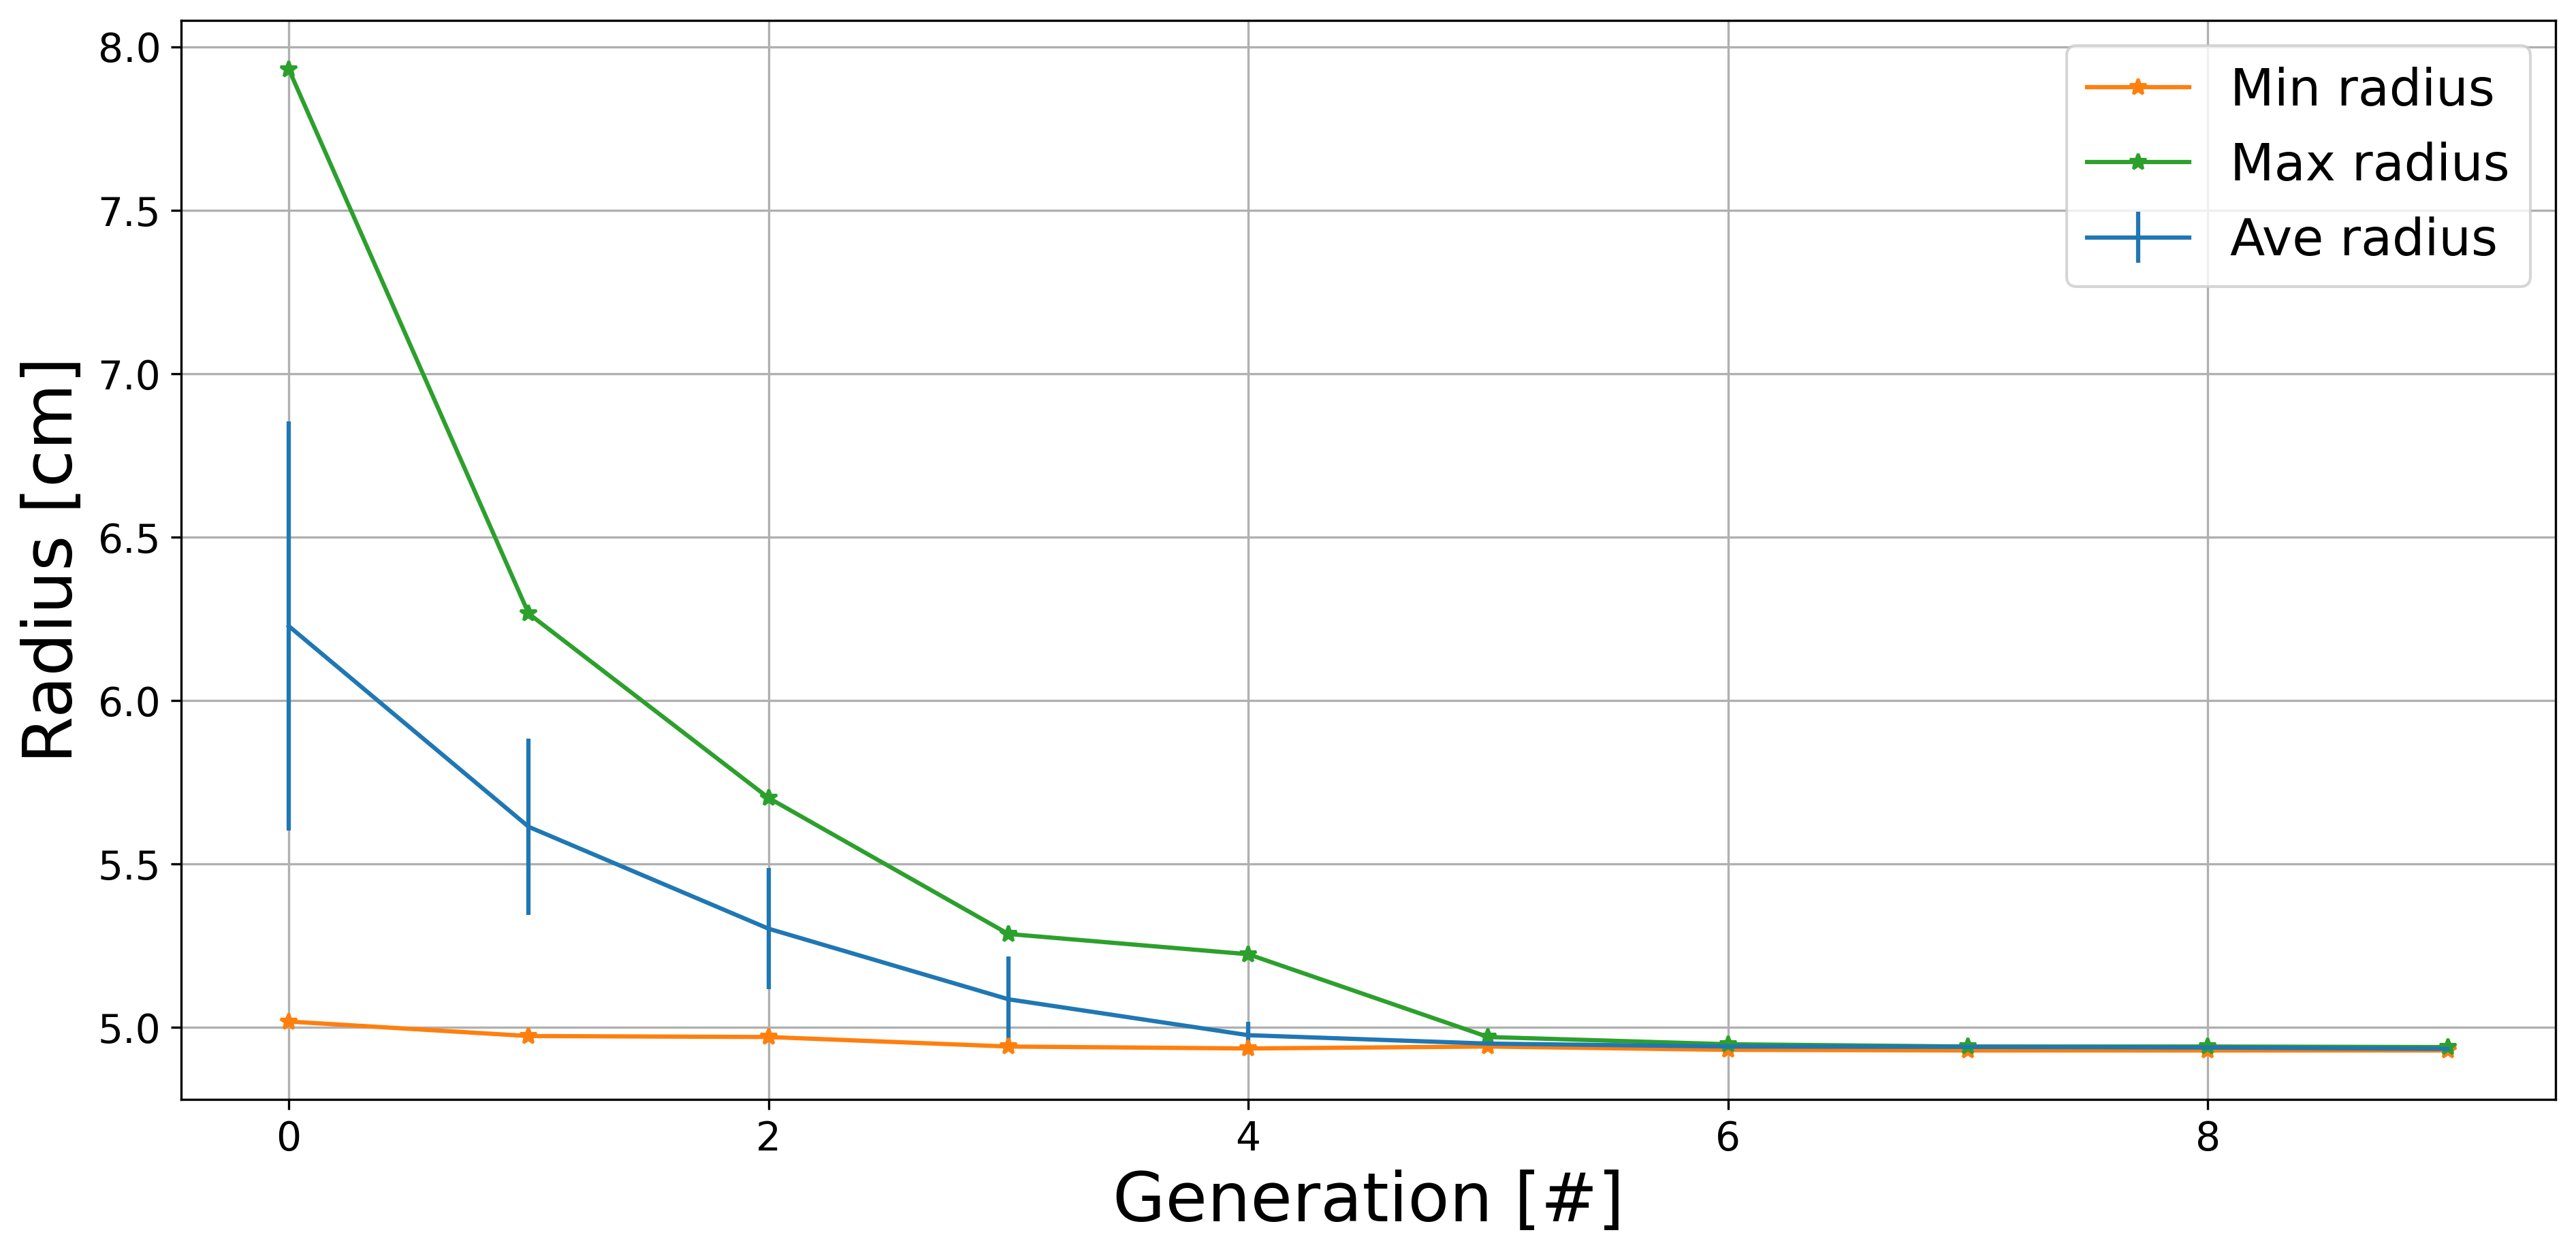
\includegraphics[width=1.1\linewidth]{radius-convergence.png}} 
    \caption{Minimum, average, and maximum radius values evolution.}
    \label{fig:verification-radius}
    \end{subfigure}
    \begin{subfigure}{\textwidth}
        \makebox[\textwidth][c]{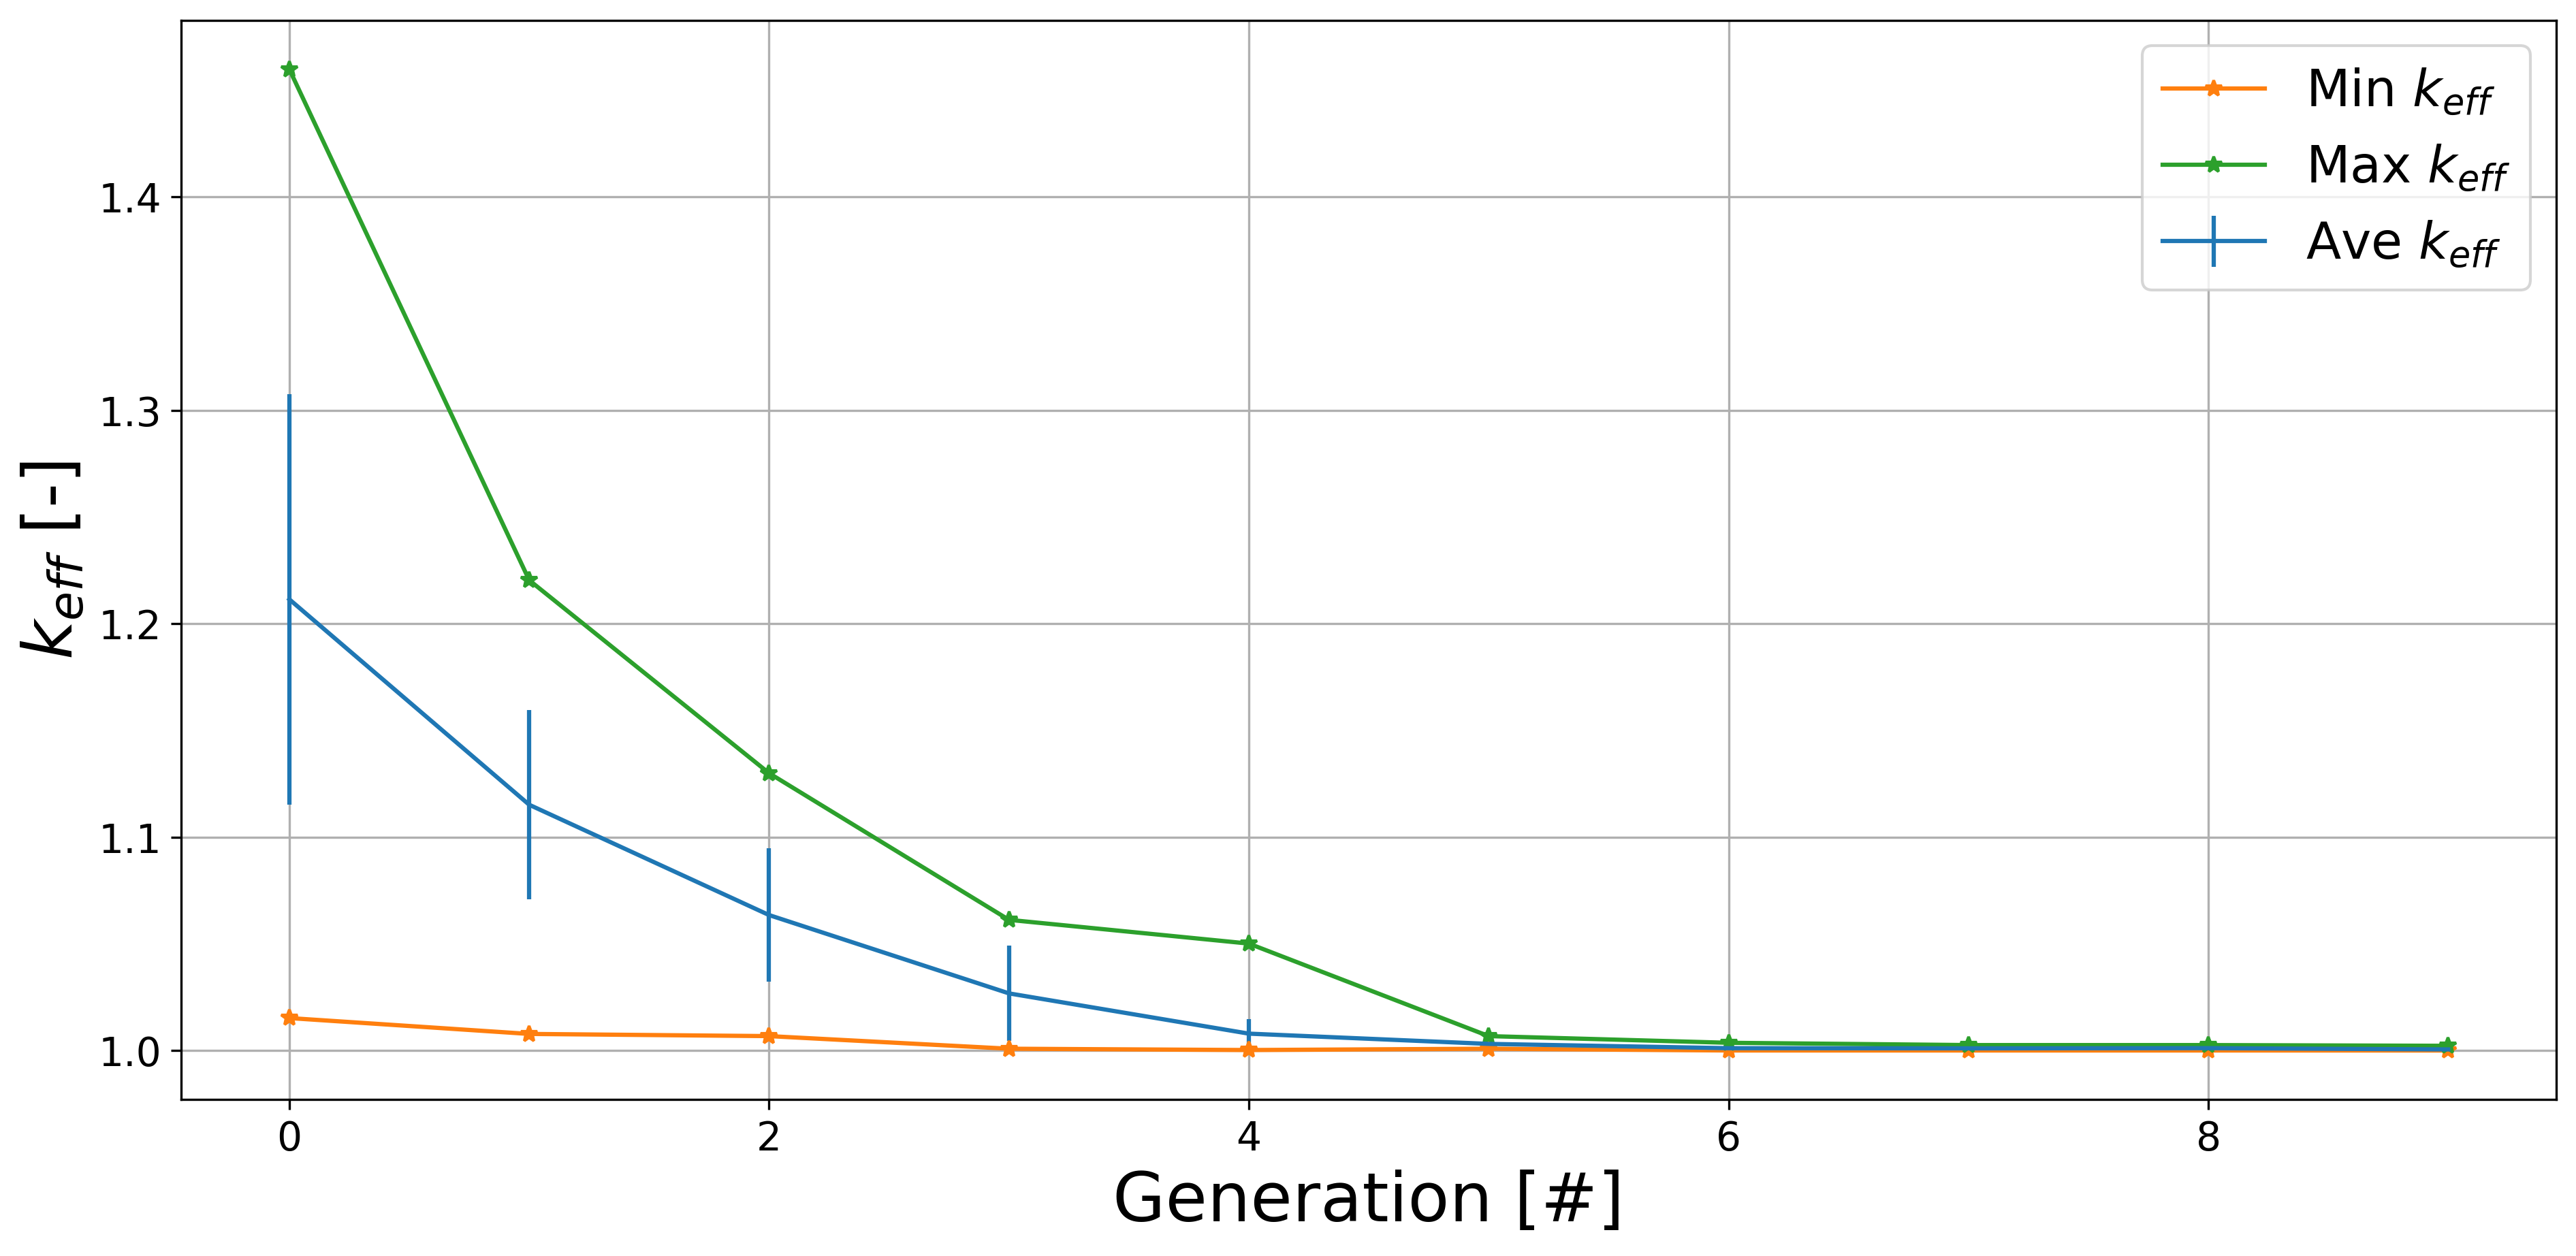
\includegraphics[width=1.1\linewidth]{keff-convergence.png}}
        \caption{Minimum, average, and maximum $k_{eff}$ values evolution.}
        \label{fig:verification-keff}
    \end{subfigure}
    \caption{Results for each generation for \gls{ROLLO}'s genetic algorithm optimization 
    to the find the critical radius of a  $^{239}Pu$ bare sphere.}
\end{figure}

\section{ROLLO Convergence Criteria}
The \texttt{generations} input parameter defines \gls{ROLLO}'s evolutionary algorithm 
convergence criterion. 
Each nuclear reactor model's evaluation is computationally intensive. 
Users will most likely be constrained by the total available compute time. 
Therefore, rather than setting a results-based stopping criterion, ROLLO enables 
users to define the \texttt{generations} and \texttt{pop$\_$size} based on the 
amount of compute time available to them: 
\begin{align}
    t_{total} &= t_{eval} \times gen \times pop 
\intertext{where}
    t_{total} &= \mbox{Total compute time available} \nonumber \\
    t_{eval} &= \mbox{compute time per nuclear reactor model evaluation} \nonumber \\
    gen &= \mbox{total number of generations in optimization process} \nonumber \\
    pop &= \mbox{population size in optimization process} \nonumber
\end{align} 

\subsection{Convergence}
\label{sec:rollo-convergence}
ROLLO does not utilize a mathematical expression to evaluate problem convergence. 
The complexity of reactor design optimization means that no single indicator determines 
if convergence is met.
Instead, ROLLO's purpose is to help the human reactor designer narrow down the design 
space. 
When a ROLLO run completes, the user plots the objectives' convergence and 
Pareto front (for multiobjective simulations) to evaluate if they are confident 
about the final solution set. 
Section \ref{sec:opt} described that an ideal optimization method for a 
multi-objective problem like reactor design should find widely spread solutions 
on the obtained Pareto front \cite{deb_multi-objective_2001}. 
If the simulation is not converged, the user can easily restart the optimization 
simulation using the \texttt{checkpoint.pkl} file and run the problem for a few more 
generations. 
% add about hypervolume for multiobj and obj convergence for singleobj

\section{Summary}
This chapter described the \acrfull{ROLLO} framework developed for 
this dissertation. 
\gls{ROLLO} is a Python package that applies evolutionary algorithm 
optimization techniques to nuclear reactor design using the \acrfull{DEAP} 
module. 
The motivation for \gls{ROLLO} is to enable reactor designers to utilize 
robust evolutionary algorithm optimization methods without going 
through the cumbersome process of setting up a genetic algorithm framework,
selecting appropriate hyperparameters, and setting up its parallelization. 
I designed \gls{ROLLO} to be effective, flexible, open-source, parallel, 
reproducible, and usable. 
\gls{ROLLO} is hosted on Github \cite{chee_rollo_2021}. 
\section{ROLLO Verification}
To verify \gls{ROLLO}'s optimization capabilities, I conducted multiple verification 
studies: commonly used evolutionary algorithm single and multi objective benchmark problems
and a nuclear reactor-specific problem. 
Together, they prove that \gls{ROLLO}'s evolutionary algorithm is correctly implemented 
and suitable for conducting nuclear reactor optimization problems. 

\subsection{Ackley Function}
The Ackley function is a non-convex function, commonly used as a performance test 
for single-objective optimization algorithms \cite{ackley_connectionist_2012}: 
\begin{align}
    f(x) &= -a \cdot exp \left(-b\sqrt{\frac{1}{d}\Sigma_{i=1}^dx_i^2}\right) - 
    exp \left(\frac{1}{d}\Sigma_{i=1}^d cos(cx_i)\right) + a + exp(1) 
\end{align}
The recommended variable values are $a=20$, $b=0.2$, and $c=2\pi$
\cite{sfu_ackley_nodate}. 
The Ackley function's global optimum point is $f(0,0) = 0$. 
Figure \ref{fig:ackley} shows the resulting two-variable Ackley function.
\begin{figure}[H]
    \centering
    \includegraphics[width=0.65\linewidth]{figures/ackley.png} 
    \caption{Two variable Ackley function \cite{sfu_ackley_nodate}.}
    \label{fig:ackley}
\end{figure}
 
I added an integration test to \gls{ROLLO} that checks that a default \gls{ROLLO} 
simulation will find the Ackley function's global optimum point. 
If \gls{ROLLO} performed sub-optimally, it would return one of the Ackley 
function's many local minimums. 
\gls{ROLLO} successfully finds the global optimum point, and thus passes the 
integration test. 

\subsection{Binh and Korn Function}
The Binh and Korn function is a two-objective function:
\begin{align}
    Minimize = \begin{cases}
        f_1 (x,y) &= 4x^2+4y^2 \\
        f_2 (x,y) &= (x-5)^2 + (y-5)^2
    \end{cases}
\end{align}
We use it as a performance test for dual-objective optimization.
Figure \ref{fig:binh} shows the Binh and Korn function's pareto front.
I use the hypervolume indicator to quantify the goodness of 
pareto front. 
The hypervolume indicator is one of the most used set-quality indicators for the 
assessment of stochastic multiobjective optimizers \cite{guerreiro_hypervolume_2020}.
% describe hypervolume
I added an integration test to ROLLO that checks that a ROLLO simulation will 
find a hypervolume comparable to the ideal pareto front when minimizing the
Binh and Korn function. 


\subsection{Pu-239 Critical Bare Sphere}
To ensure \gls{ROLLO} works correctly while coupled with OpenMC, I run \gls{ROLLO} 
to find the critical radius for a $^{239}Pu$ bare sphere. 
The solution to this problem is well studied and available \cite{blanchard_updated_1999}. 
Blanchard et al reported that with MCNP4b code and ENDF/B-VI data library, the 
critical mass of a Pu239 bare sphere is 10.00 kg which corresponds to a diameter 
of 9.9cm \cite{blanchard_updated_1999}.
Figure \ref{fig:verification-sphere} shows the ROLLO input file for this verification 
problem. 
In the input file, I vary the radius between 1.0 and 8.0cm, with the objective of 
minimizing radius, while constraining the problem to have $k_{eff} >= 1.0$.
\begin{figure}[H]
    \begin{minted}[
        frame=lines,
        framesep=2mm,
        baselinestretch=1.2,
        fontsize=\footnotesize,
        linenos
        ]{json}
        {"control_variables": {
                "radius": {"min": 1.0, "max": 8.0}},
            "evaluators": {
                "openmc": {
                    "input_script": "critical_sphere.py",
                    "inputs": ["radius"],
                    "outputs": ["keff", "radius"],
                    "keep_files": false}},
            "constraints": {"keff": {"operator": [">="], "constrained_val": [1.0]}},
            "algorithm": {
                "parallel": "multiprocessing",
                "objective": ["min"],
                "optimized_variable": ["radius"]
            }}
    \end{minted}
    \caption{\acrfull{ROLLO} JSON input file for finding the minimum radius for 
    a $^{239}Pu$ Critical Bare Sphere.}
    \label{fig:verification-sphere}
\end{figure}
\pagebreak
Figure \ref{fig:critical_sphere.py} shows the OpenMC template used in the 
\gls{ROLLO} simulation. 
\begin{figure}[H]
    \begin{minted}[
        frame=lines,
        framesep=2mm,
        baselinestretch=1.2,
        fontsize=\footnotesize,
        linenos
        ]{python}
            import openmc 
            import numpy as np

            pu = openmc.Material()
            pu.set_density("g/cm3", 19.84)
            pu.add_nuclide("Pu239", 1)
            mats = openmc.Materials([pu])
            
            radius = {{radius}}
            
            fuel_sphere = openmc.Sphere(r=radius, boundary_type='vacuum')
            fuel_cell = openmc.Cell(fill=pu, region=-fuel_sphere)
            univ = openmc.Universe(cells=[fuel_cell])
            geom = openmc.Geometry(univ)
            
            settings = openmc.Settings()
            settings.batches = 100
            settings.inactive = 20
            settings.particles = 20000
            settings.temperature = {"multipole": True, "method": "interpolation"}
            
            mats.export_to_xml()
            geom.export_to_xml()
            settings.export_to_xml()
            openmc.run()
    \end{minted}
    \caption{OpenMC template input file used in ROLLO simulation to find the 
    minimum radius for a $^{239}Pu$ Critical Bare Sphere.}
    \label{fig:critical_sphere.py}
\end{figure}  

\gls{ROLLO} successfully finds the critical radius of the $^{239}Pu$ bare sphere 
to be 4.9856cm which corresponds to approximately a 9.9cm diameter. 
The critical sphere's $k_{eff}$ value is 1.00919 $\pm$ 0.00048. 
Figure \ref{fig:verification-radius} and \ref{fig:verification-keff} show the 
radius and $k_{eff}$ evolution through the evolutionary algorithm's 
generations. 
They demonstrate how the average radius and $k_{eff}$ converge
towards the critical radius while keeping $k_{eff} > 1$ with improvements from 
each generation.
\begin{figure}[]
    \centering
    \begin{subfigure}{\textwidth}
    \makebox[\textwidth][c]{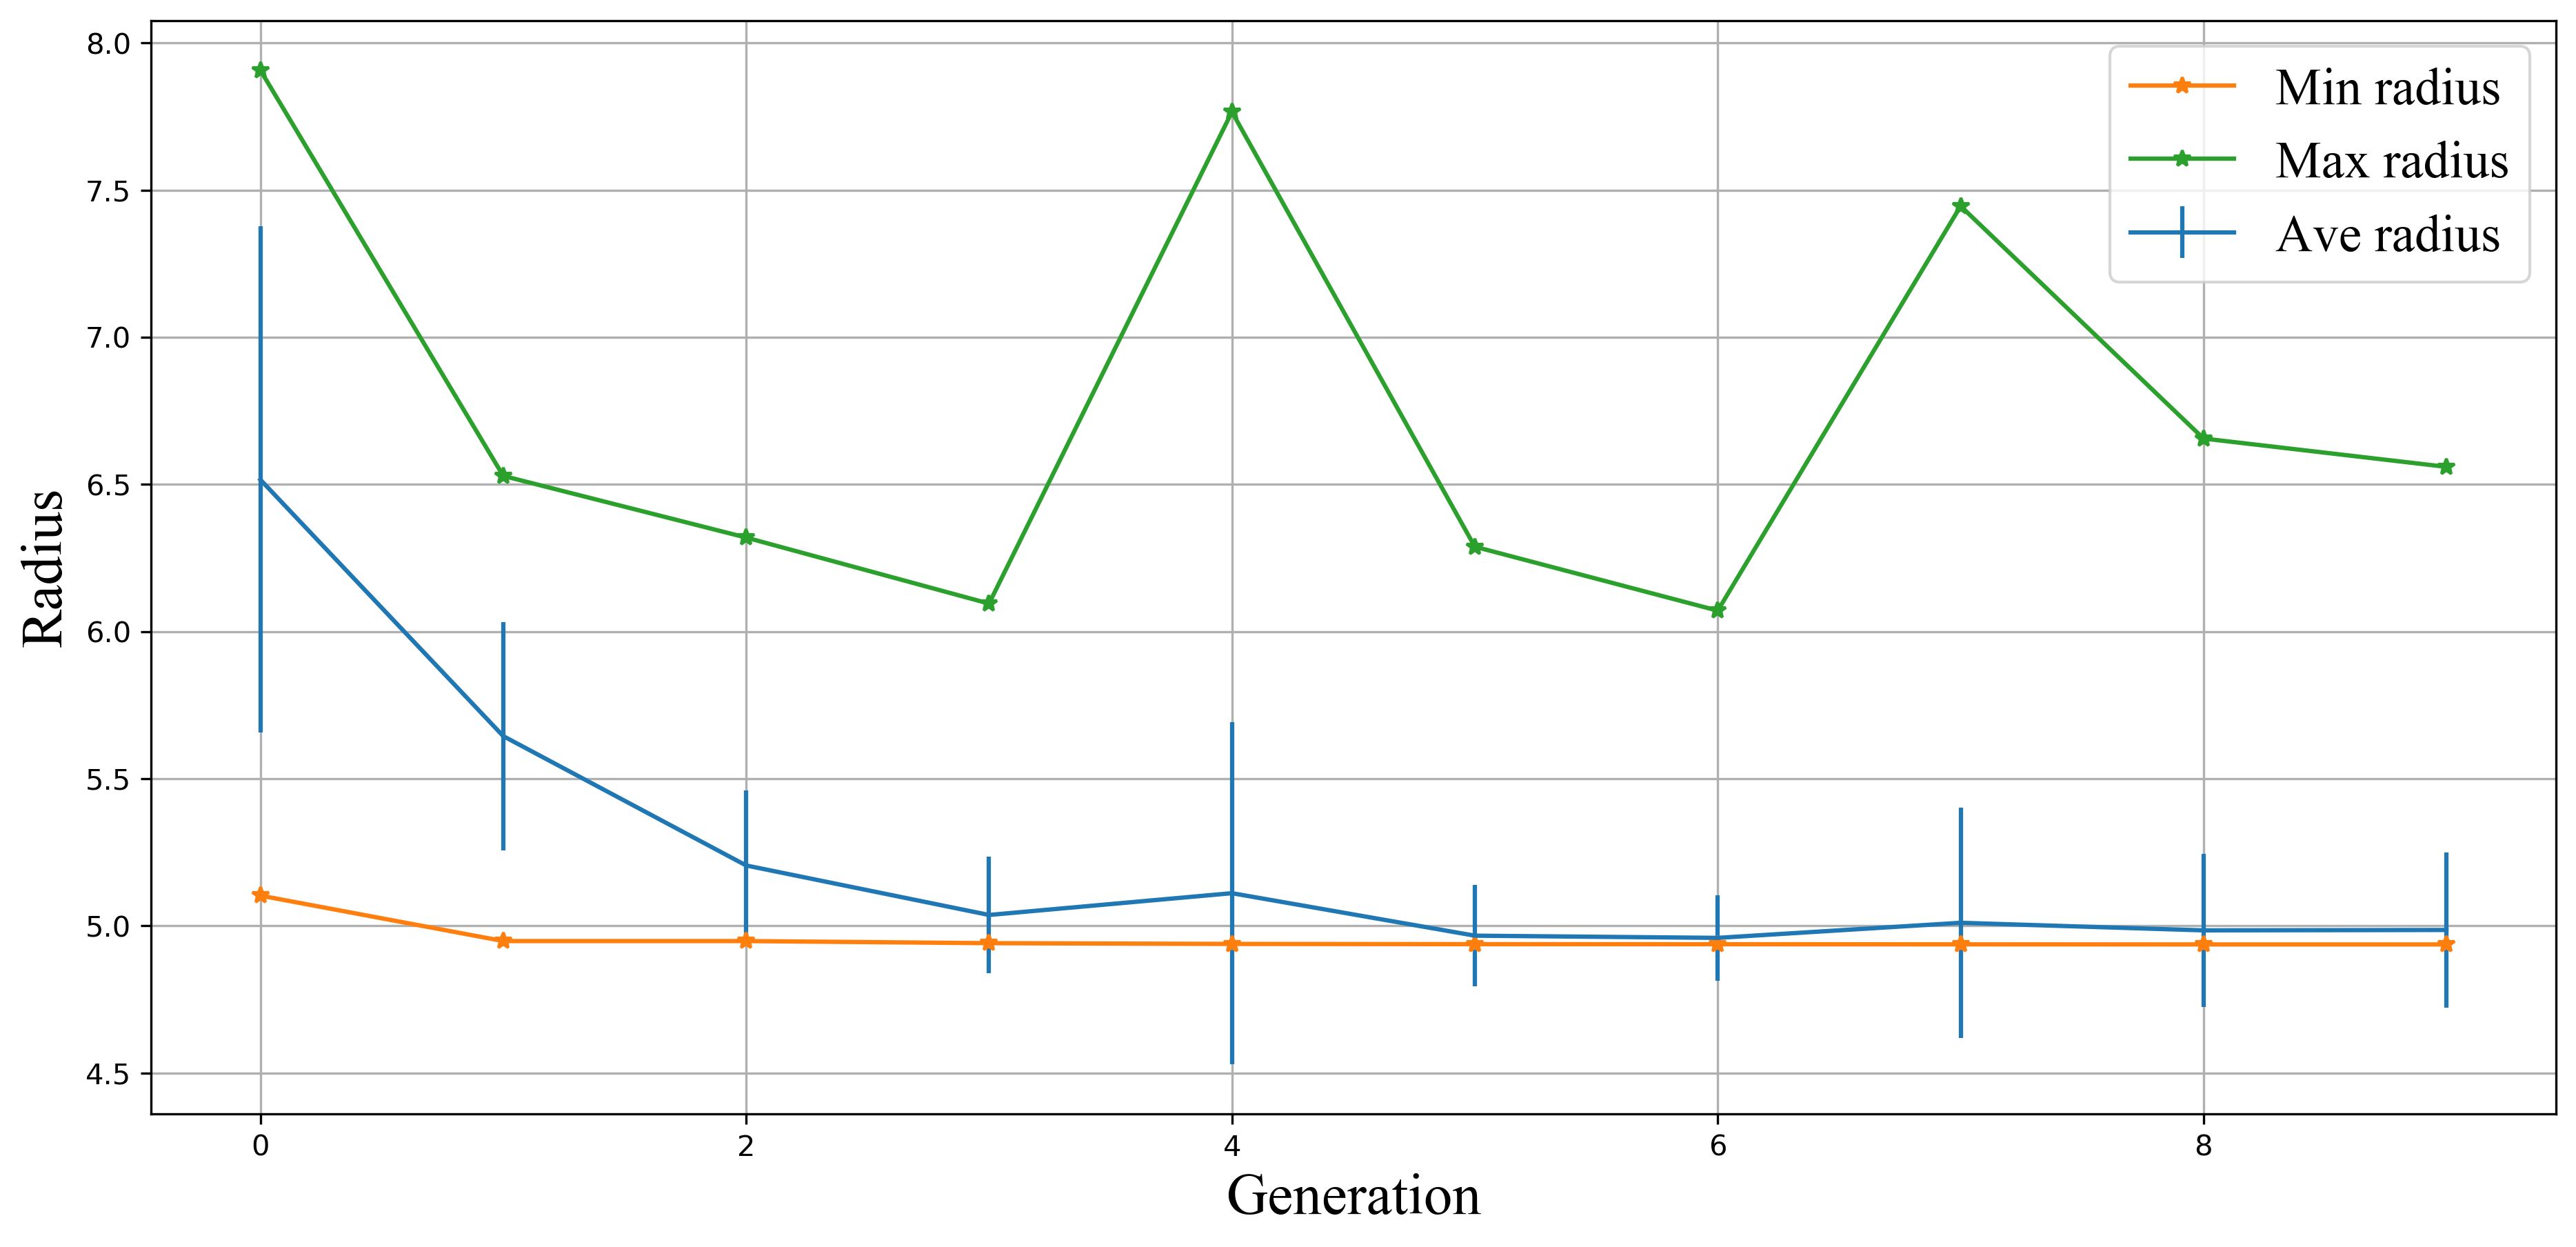
\includegraphics[width=1.1\linewidth]{verification-radius.png}} 
    \caption{Minimum, average, and maximum radius values evolution.}
    \label{fig:verification-radius}
    \end{subfigure}
    \begin{subfigure}{\textwidth}
        \makebox[\textwidth][c]{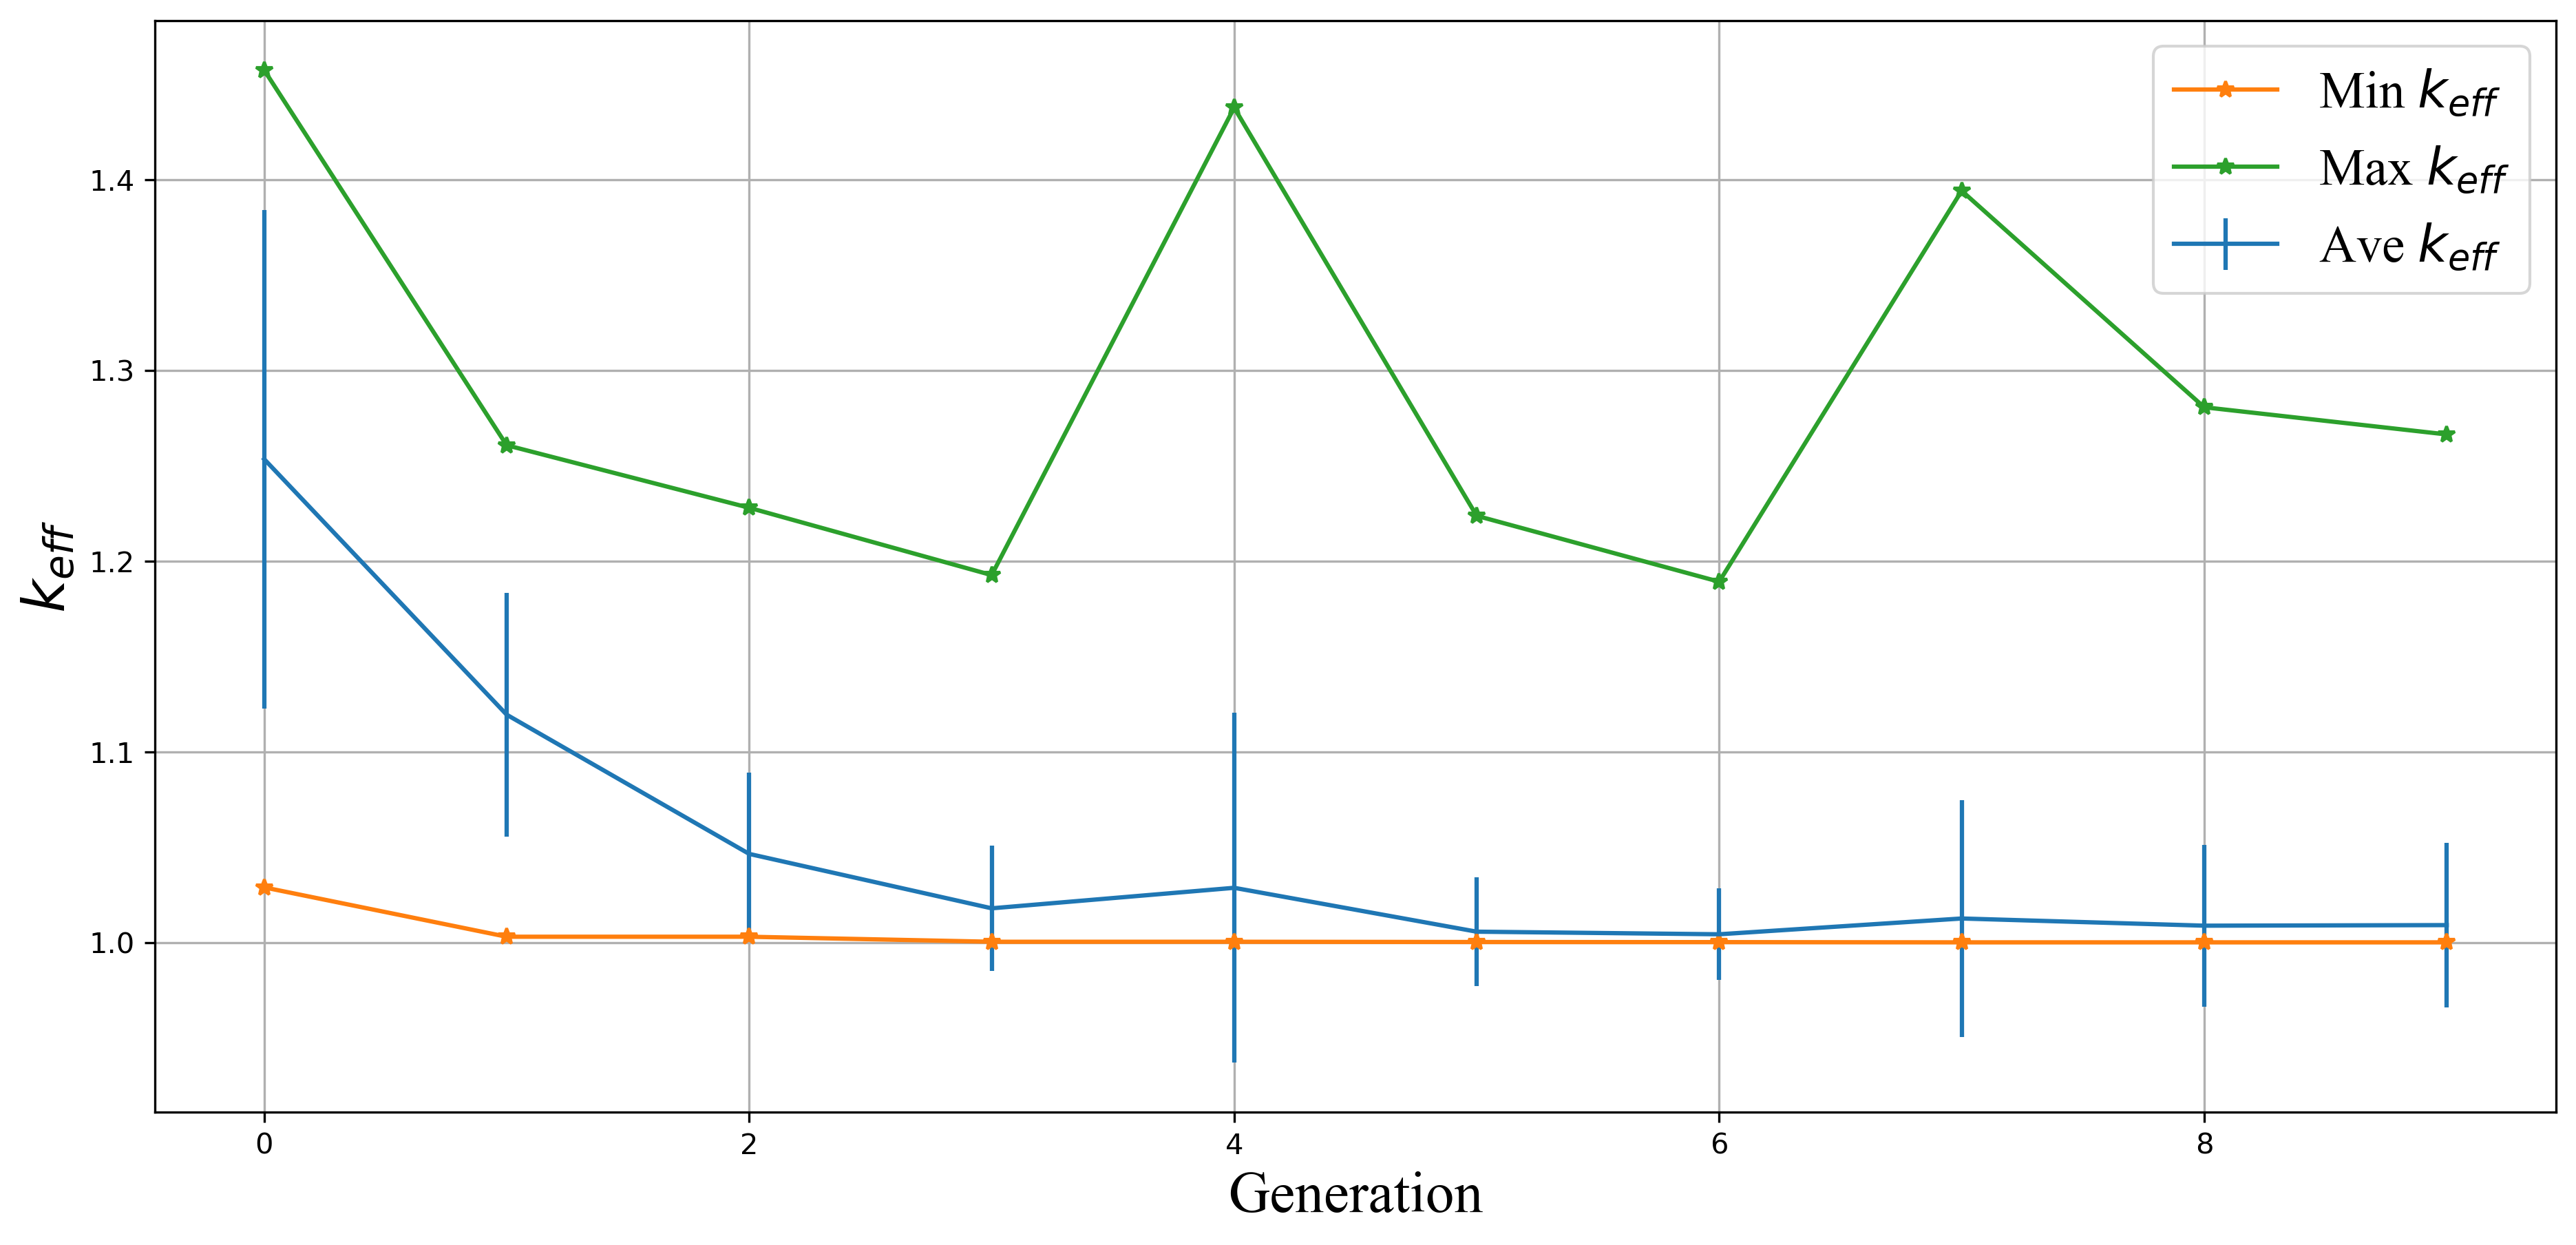
\includegraphics[width=1.1\linewidth]{verification-keff.png}}
        \caption{Minimum, average, and maximum $k_{eff}$ values evolution.}
        \label{fig:verification-keff}
    \end{subfigure}
    \caption{Results for each generation for \gls{ROLLO}'s genetic algorithm optimization 
    to the find the critical radius of a  $^{239}Pu$ bare sphere.}
\end{figure}
\chapter{AHTR Plank Optimization Results}
\glsresetall
\label{chap:ahtr-plank-opt-results}
In this chapter, I report the \gls{AHTR} plank's \gls{ROLLO} optimization results. 
I vary the following \gls{AHTR} plank input parameters:
\begin{itemize}
    \item \gls{TRISO} packing fraction distribution ($\rho_{TRISO}(\vec{r})$)
    \item Total fuel packing fraction ($PF_{total}$)
    \item Coolant channel shape
\end{itemize} 
And, I optimize the \gls{AHTR} plank for the following optimization objectives:
\begin{itemize}
    \item Minimize total fuel packing fraction ($PF_{total}$)
    \item Minimize maximum plank temperature ($T_{max}$)
    \item Minimize fuel-normalized power peaking factor ($PPF_{fuel}$)
\end{itemize} 

In the previous chapter, I detailed the methodology for \gls{AHTR} plank modeling and 
\gls{ROLLO} optimization. 
Section \ref{sec:ahtr-plank-geometry} describes the \gls{AHTR} plank geometry.
Section \ref{sec:input-parameter-modeling} details about how I vary the 
\gls{AHTR} plank's input parameters. 
Sections \ref{sec:ahtr-moltres-hom} and \ref{sec:ahtr_model_verification}
describe and verify the \gls{AHTR} plank's OpenMC neutronics and Moltres 
temperature models. 
Section \ref{sec:opt-problem} describes the optimization objectives and Section 
\ref{sec:ahtr_slab_output} describes how I calculated them from the OpenMC and Moltres 
model outputs. 
Section \ref{sec:hyperparameter-studies} describes the hyperparameter tuning process 
to select hyperparameters for the single-objective and multi-objective \gls{ROLLO} 
optimization simulations.

The subsequent sections outline the \gls{AHTR} plank optimization simulations, describe 
the results of the single-objective and multi-objective \gls{ROLLO} optimization 
simulations, report each simulation's computational cost, and discuss the results' 
significance.

\section{ROLLO AHTR Plank Optimization Simulations Overview}
Table \ref{tab:slab-obj-breakdown} shows the details of each \gls{ROLLO} 
optimization simulation explored in this chapter.
\begin{table}[htbp!]
    \centering
    \onehalfspacing
    \caption{\acrfull{ROLLO} simulations for optimizing \acrfull{AHTR}
    plank. $PF_{total}$: Total fuel packing fraction, $T_{max}$: Maximum plank temperature, 
    $PPF_{fuel}$: Fuel-normalized power peaking factor, $\rho_{TRISO}(\vec{r})$: 
    \gls{TRISO} particle distribution}
	\label{tab:slab-obj-breakdown}
    \footnotesize
    \begin{tabular}{p{1cm}|p{1cm}|llll}
    \hline 
    \textbf{Objs} & \textbf{Sim} & \textbf{Objectives} & \textbf{Constraints} &\textbf{Varying Parameters} & \textbf{Simulation Software} \\
    \hline
    \multirow{7}{2cm}{1} & p-1a & \tabitem min($PF_{total}$) & \tabitem $k_{eff}$ $\geq$ 1.35 &\tabitem $\rho_{TRISO}(\vec{r})$ & OpenMC \\
    & & & & \tabitem $PF_{total}$ & \\
    \cline{2-6}
    & p-1b & \tabitem min($T_{max}$) & \tabitem $k_{eff}$ $\geq$ 1.0 &\tabitem $\rho_{TRISO}(\vec{r})$ & OpenMC, Moltres\\
    \cline{2-6}
    & p-1c & \tabitem min($PPF_{fuel}$) & \tabitem $k_{eff}$ $\geq$ 1.0 &\tabitem $\rho_{TRISO}(\vec{r})$ & OpenMC\\
    \cline{2-6}
    & p-1d & \tabitem min($PF_{total}$) & \tabitem $k_{eff}$ $\geq$ 1.35 &\tabitem Coolant channel shape & OpenMC \\
    & & & & \tabitem $PF_{total}$ & \\
    \cline{2-6}
    & p-1e & \tabitem min($T_{max}$) & \tabitem $k_{eff}$ $\geq$ 1.35 &\tabitem Coolant channel shape & OpenMC, Moltres\\
    \cline{2-6}
    & p-1f & \tabitem min($PPF_{fuel}$) & \tabitem $k_{eff}$ $\geq$ 1.35 &\tabitem Coolant channel shape & OpenMC\\
    \hline
    \multirow{6}{2cm}{2}& p-2a & \tabitem min($PF_{total}$) & \tabitem $k_{eff}$ $\geq$ 1.35 & \tabitem $\rho_{TRISO}(\vec{r})$ & OpenMC, Moltres\\
    & &\tabitem min($T_{max}$) & & \tabitem $PF_{total}$ & \\
    \cline{2-6}
    & p-2b & \tabitem min($PF_{total}$) & \tabitem $k_{eff}$ $\geq$ 1.35 & \tabitem $\rho_{TRISO}(\vec{r})$ & OpenMC\\
    & & \tabitem min($PPF_{fuel}$) & & \tabitem $PF_{total}$ & \\
    \cline{2-6}
    & p-2c & \tabitem min($T_{max}$) & \tabitem $k_{eff}$ $\geq$ 1.0 & \tabitem $\rho_{TRISO}(\vec{r})$ & OpenMC, Moltres\\
    & & \tabitem min($PPF_{fuel}$) & & & \\
    \hline
    \multirow{6}{2cm}{3}& p-3a &\tabitem min($PF_{total}$) & \tabitem $k_{eff}$ $\geq$ 1.35 & \tabitem $\rho_{TRISO}(\vec{r})$ & OpenMC, Moltres\\
    && \tabitem min($PPF_{fuel}$) & & \tabitem $PF_{total}$ & \\
    && \tabitem min($T_{max}$) & & & \\
    \cline{2-6}
    & p-3b &\tabitem min($PF_{total}$) & \tabitem $k_{eff}$ $\geq$ 1.35 & \tabitem $\rho_{TRISO}(\vec{r})$ & OpenMC, Moltres\\
    && \tabitem min($PPF_{fuel}$) & & \tabitem $PF_{total}$ & \\
    && \tabitem min($T_{max}$) & & \tabitem Coolant channel shape& \\
    \hline
    \end{tabular}
\end{table}

I first conducted single objective, single input parameter \gls{ROLLO} optimizations to 
understand the individual impacts of each objective on each input parameter. 
Their results will inform the multi-objective optimization simulations setup. 

The $k_{eff}$ constraint value is 1.35 and 1.0 for optimization problems that do
and do not minimize total packing fraction, respectively. 
$k_{eff}$ is strongly correlated with total packing fraction. 
The \gls{AHTR} plank with the same packing fraction as the \gls{FHR} Benchmark's assembly 
model had a $k_{eff}$ of 1.35, thus, I constrainined $k_{eff} \geq 1.35$ to find optimal 
input parameters that achieve similar performance to the original benchmark \gls{TRISO} 
distribution. 

Simulations are run on the BlueWaters supercomputer \cite{ncsa_about_2017} and Theta 
supercomputer at the Argonne Leadership Computing Facility under the Director's 
Discretionary Allocation Program \cite{noauthor_argonne_2022}. 
Section \ref{sec:plank-compute-cost} details each optimization simulation's computational 
cost.  

\section{AHTR Plank: Single-Objective Optimization Results}
\label{sec:plank-one-obj}
In this section, I report the \gls{AHTR} plank's \gls{ROLLO} single-objective 
optimization results. 
Table \ref{tab:slab-obj-breakdown} summarized the one-objective simulations in this
section: p-1a, p-1b, p-1c, p-1d, p-1e, and p-1f. 
In the following subsections, I describe the single-objective optimization results 
grouped by the minimized objective. 

If a single-objective optimization problem's objective converges earlier than the 
5 generations I intended to run (determined in Section 
\ref{sec:multi-obj-hyperparameters}), I stop running the simulation at that generation. 

\subsection{Objective: Minimize Total Packing Fraction ($PF_{total}$)}
This section reports results from the minimize total fuel packing fraction 
($PF_{total}$) single-objective optimization simulations: p-1a and p-1d. 
Simulation p-1a varies total fuel packing fraction and \gls{TRISO} packing fraction 
distribution ($\rho_{TRISO}(\vec{r})$), while simulation p-1d varies the total fuel 
packing fraction ($PF_{total}$) and coolant channel shape. 

\subsubsection{Simulation p-1a: Variation of $\rho_{TRISO}(\vec{r})$ and $PF_{total}$}
Table \ref{tab:simulationp1a} shows simulation p-1a's optimization problem parameters. 
\begin{table}[htbp!]
    \centering
    \onehalfspacing
    \caption{Simulation p-1a optimization problem parameters.}
	\label{tab:simulationp1a}
    \footnotesize
    \begin{tabular}{l|p{5cm}}
    \hline 
    \multicolumn{2}{c}{\textbf{Single Objective: Simulation p-1a}} \\
    \hline 
    \textbf{Objectives} & Minimize $PF_{total}$ \\
    \hline 
    \textbf{Input parameter variations} & $0.02<PF_{total}<0.04$ \\
    & $0<a<2$ \\
    & $0<b<\frac{\pi}{2}$ \\
    & $0<c<2\pi$ \\
    \hline
    \textbf{Constraints} & $k_{eff} \geq 1.35$\\ 
    \hline 
    \textbf{Genetic algorithm parameters} & Population size: 60 \\
    & Generations: 10 \\
    \hline
    \end{tabular}
\end{table}

Figure \ref{fig:slab-obj-1-pf-evol} shows the $PF_{total}$ evolution,  
Figure \ref{fig:slab-obj-1-pf-final} shows the five TRISO packing fraction 
distributions ($\rho_{TRISO}(\vec{r})$) in the final generation with the 
most-minimized $PF_{total}$, and Figure \ref{fig:slab-obj-1-pf-most-minimized} 
illustrates the \gls{AHTR} plank model with most-minimized $PF_{total}$.
\begin{figure}[htbp!]
    \centering
    \begin{subfigure}{0.95\textwidth}
        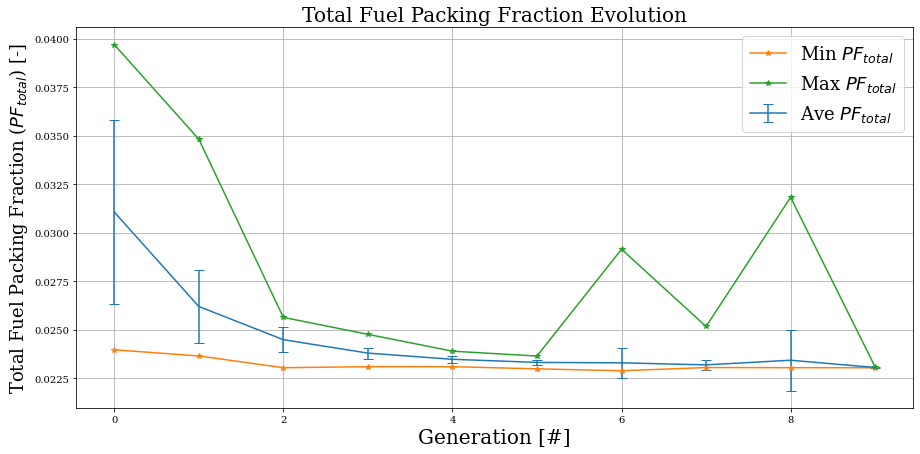
\includegraphics[width=\linewidth]{slab-obj-1-pf-evol.png}
        \caption{Minimum, average, and maximum $PF_{total}$ evolution.}
        \label{fig:slab-obj-1-pf-evol} 
    \end{subfigure}
    \begin{subfigure}{0.95\textwidth}
        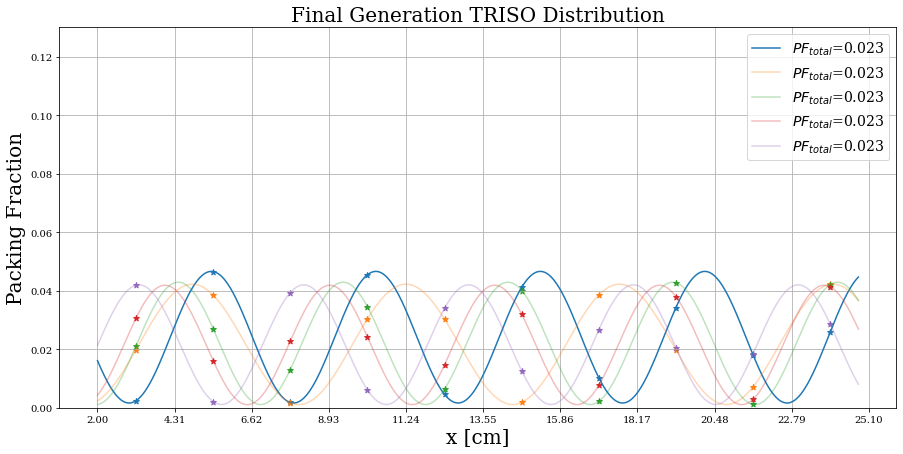
\includegraphics[width=\linewidth]{slab-obj-1-pf-final.png}
        \caption{TRISO packing fraction distribution for the 5 reactor models with the 
        smallest $PF_{total}$ in the final generation.}
        \label{fig:slab-obj-1-pf-final} 
    \end{subfigure}
    \begin{subfigure}{0.95\textwidth}
        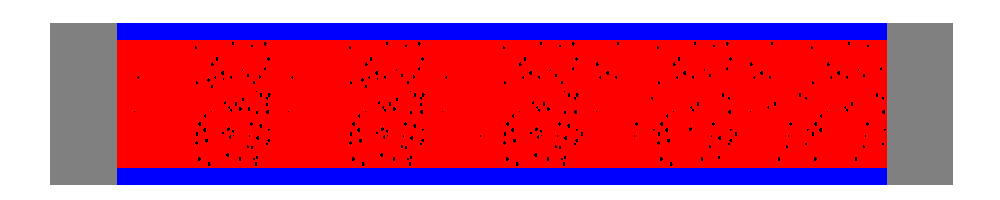
\includegraphics[width=\linewidth]{slab-obj-1-pf-most-minimized.png}
        \caption{\gls{AHTR} plank model with most-minimized $PF_{total}$ 
        (corresponds to the blue bolded distribution in the above plot).}
        \label{fig:slab-obj-1-pf-most-minimized} 
    \end{subfigure}
    \caption{Simulation p-1a -- ROLLO single-objective optimization to minimize total 
    fuel packing fraction. Input parameters varied: total fuel packing fraction 
    ($PF_{total}$), \gls{TRISO} packing fraction distribution ($\rho_{TRISO}(\vec{r})$).}
    \label{fig:slab-obj-1-pf}
\end{figure}

Figure \ref{fig:slab-obj-1-pf-evol} shows that the minimum and average $PF_{total}$ 
converged very quickly, as expected in this single-objective optimization 
problem.
By the final generation, the average, minimum, and maximum $PF_{total}$
values converged to approximately 0.023. 
In Figure \ref{fig:slab-obj-1-pf-final}, the \gls{TRISO} packing fraction
sine distributions are not exactly the same, but follow a similar pattern of 
alternating between a higher packing fraction, and a lower packing fraction 
in the neighboring fuel cell. 
The oscillating fuel packing pattern minimizes self-shielding effects, enabling  
a lower packing fraction for the same $k_{eff}$. 

\subsubsection{Simulation p-1d: Variation of $PF_{total}$ and Coolant channel shape}
Table \ref{tab:simulationp1d} shows simulation p-1d's optimization problem parameters. 
\begin{table}[htbp!]
    \centering
    \onehalfspacing
    \caption{Simulation p-1d Optimization Problem Parameters}
	\label{tab:simulationp1d}
    \footnotesize
    \begin{tabular}{l|p{5cm}}
    \hline 
    \multicolumn{2}{c}{\textbf{Single Objective: Simulation p-1d}} \\
    \hline 
    \textbf{Objectives} & Minimize $PF_{total}$\\
    \hline 
    \textbf{Input parameter variations} & $0.02<PF_{total}<0.05$ \\
    & $0.05<r_{top}<0.35$ \\
    & $0.05<r_{bot}<0.35$ \\
    \hline
    \textbf{Constraints} & $k_{eff} \geq 1.35$\\ 
    \hline 
    \textbf{Genetic algorithm parameters} & Population size: 64 \\
    & Generations: 3 \\
    \hline
    \end{tabular}
\end{table}

Figure \ref{fig:slab-obj-1-pf-evol-coolant} shows the $PF_{total}$ evolution 
and Figure \ref{fig:slab-obj-1-pf-final-coolant} shows a plot of total radius 
($r_{top} + r_{bot}$) against $PF_{total}$. 
\begin{figure}[htbp!]
    \centering
    \begin{subfigure}{\textwidth}
        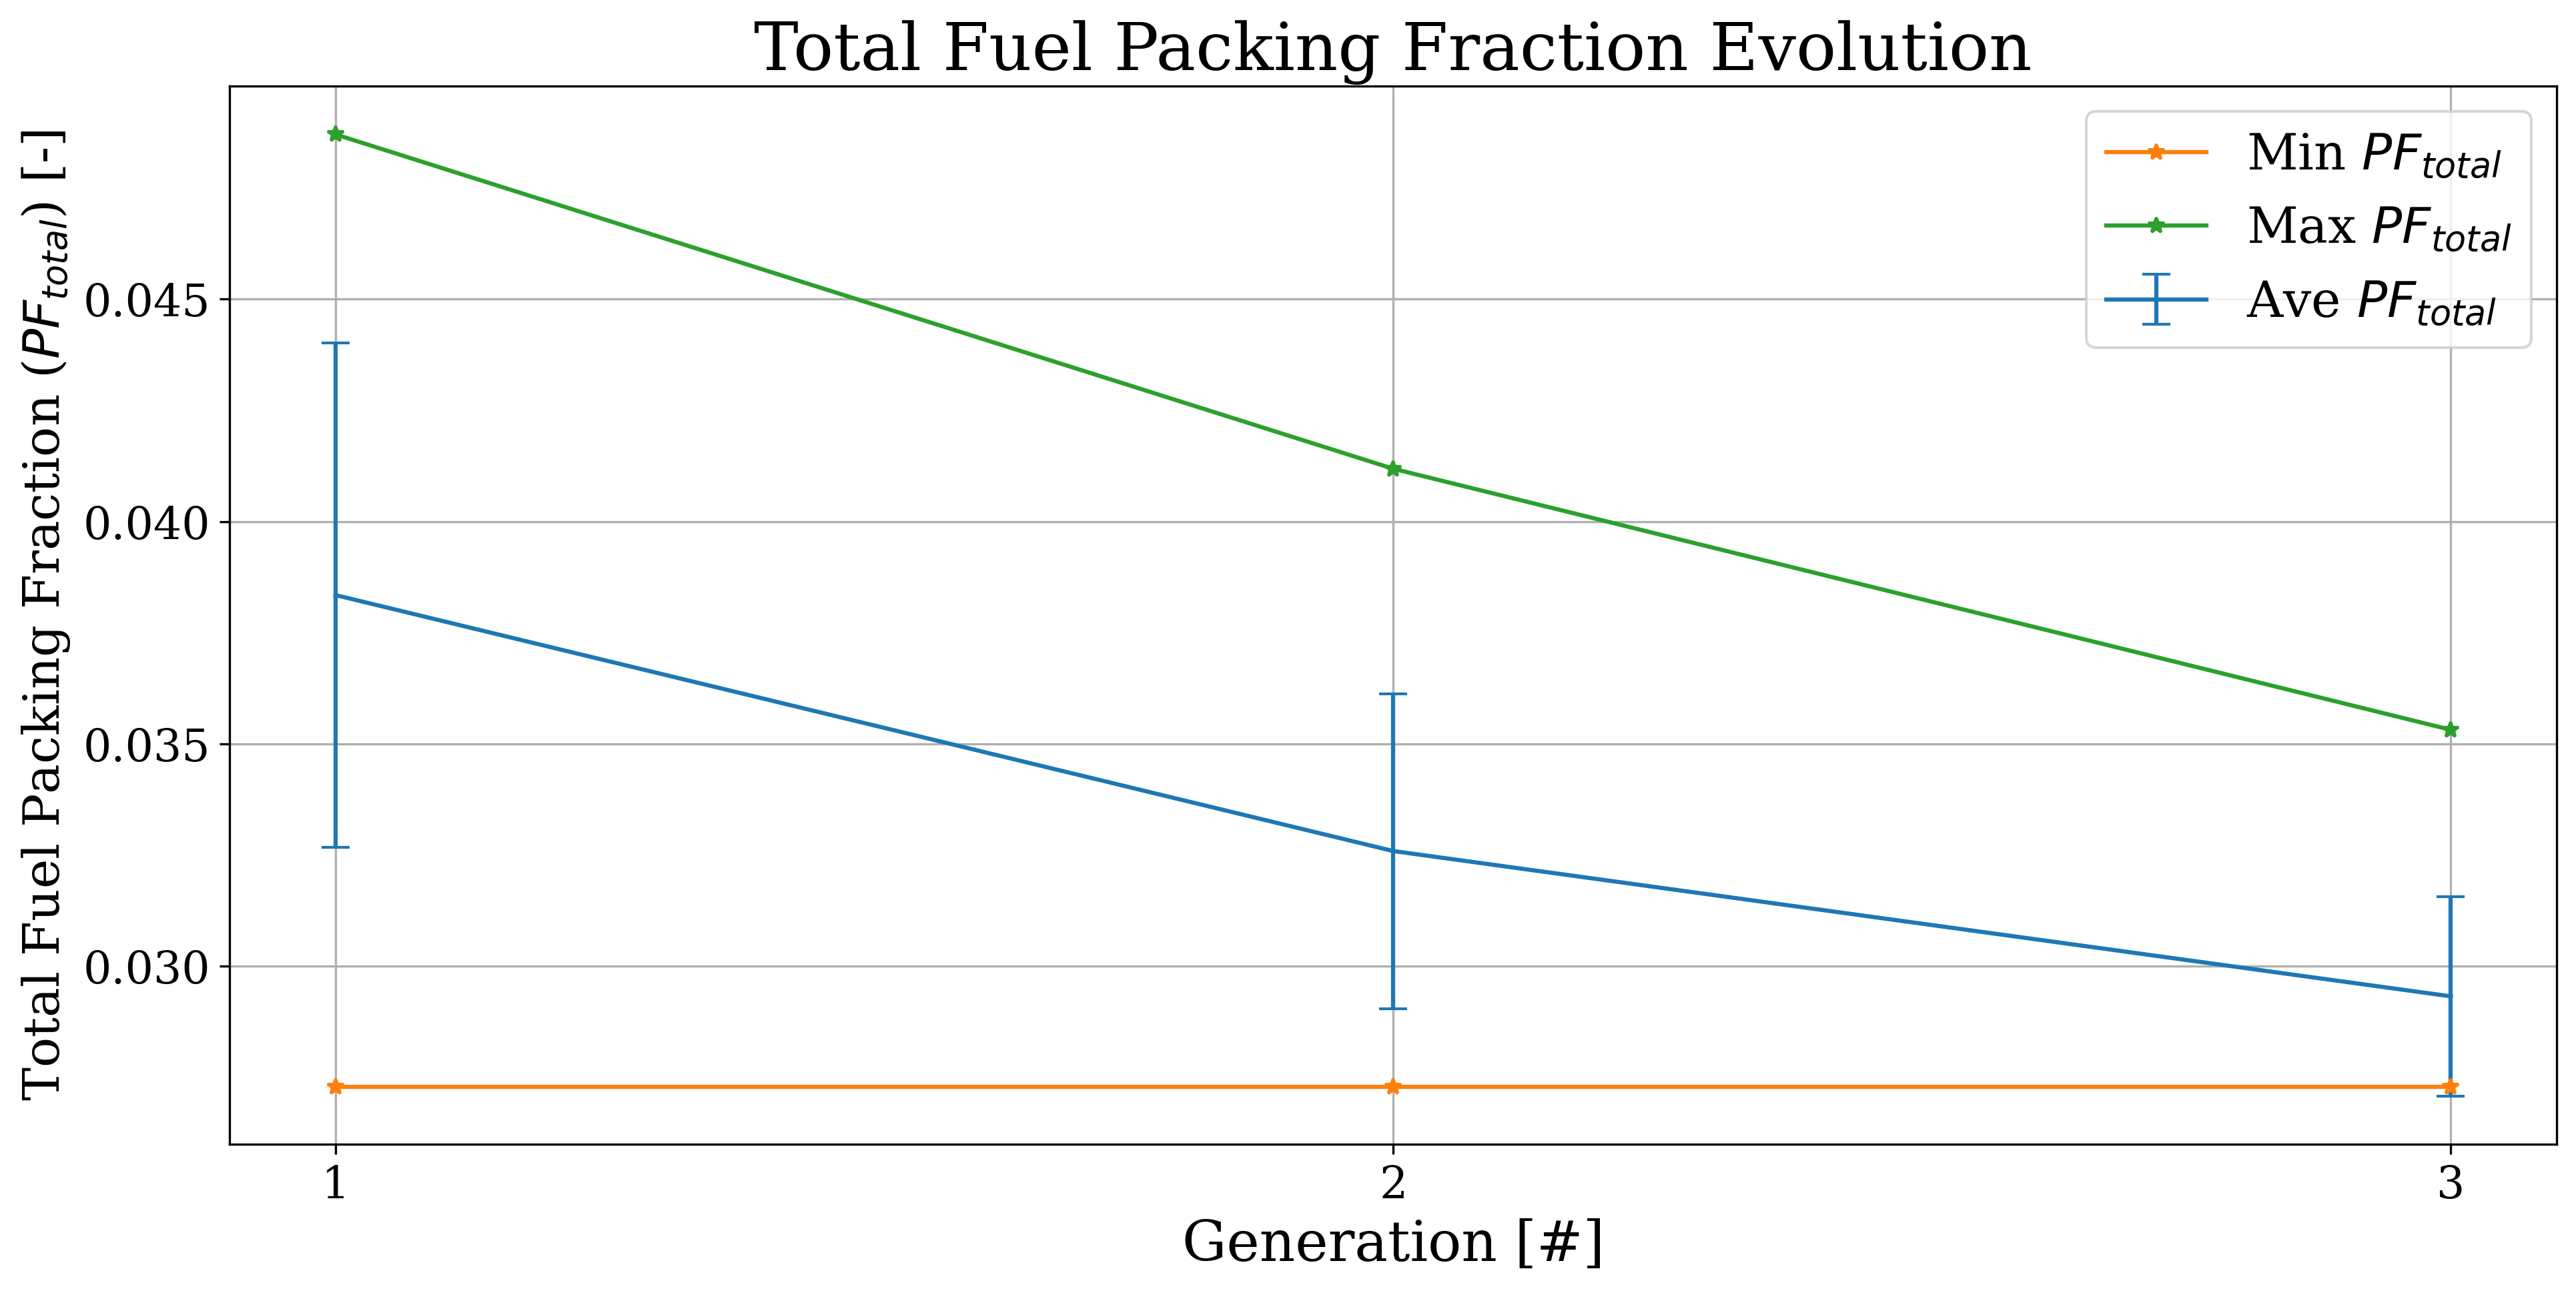
\includegraphics[width=\linewidth]{slab-obj-1-pf-evol-coolant.png}
        \caption{Minimum, average, and maximum total $PF_{total}$ evolution.}
        \label{fig:slab-obj-1-pf-evol-coolant} 
    \end{subfigure}
    \begin{subfigure}{\textwidth}
        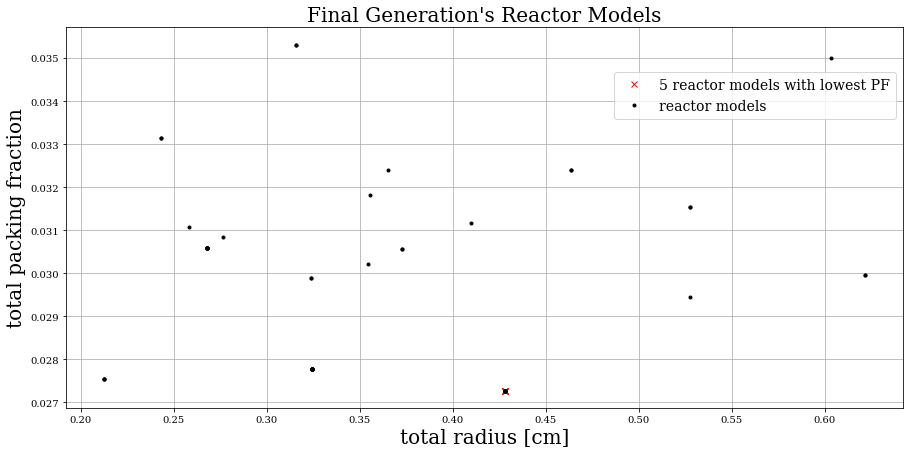
\includegraphics[width=\linewidth]{slab-obj-1-pf-final-coolant.png}
        \caption{Plot of total radius ($r_{top} + r_{bot}$) against $PF_{total}$. 
        Red crosses indicate the five reactor models with the 
        lowest $PF_{total}$.}
        \label{fig:slab-obj-1-pf-final-coolant} 
    \end{subfigure}
    \caption{Simulation p-1d -- ROLLO single-objective optimization to minimize 
    total fuel packing fraction. Input parameters varied: total fuel packing fraction 
    ($PF_{total}$), and coolant channel shape ($r_{top}, r_{bot}$).}
    \label{fig:slab-obj-1-pf-coolant}
\end{figure}
Figure \ref{fig:slab-obj-1-pf-final-coolant} demonstrates that there is no correlation 
between $PF_{total}$ and total radius. 

\subsection{Objective: Minimize Maximum Plank Temperature ($T_{max}$)}
\label{sec:plank-1-obj-temp}
This section reports results from the minimize maximum plank temperature 
($T_{max}$) single-objective optimization simulations: p-1b and p-1e. 
Simulation p-1b varies \gls{TRISO} packing fraction distribution 
($\rho_{TRISO}(\vec{r})$), while simulation p-1e varies the coolant channel shape. 

\subsubsection{Simulation p-1b: Variation of $\rho_{TRISO}(\vec{r})$}
Table \ref{tab:simulationp1b} shows simulation p-1b's optimization problem parameters. 
\begin{table}[htbp!]
    \centering
    \onehalfspacing
    \caption{Simulation p-1b Optimization Problem Parameters}
	\label{tab:simulationp1b}
    \footnotesize
    \begin{tabular}{l|p{3cm}}
    \hline 
    \multicolumn{2}{c}{\textbf{Single Objective: Simulation p-1b}} \\
    \hline 
    \textbf{Objectives} & Minimize $T_{max}$ \\
    \hline 
    \textbf{Input parameter variations} & $0<a<2$ \\
    & $0<b<\frac{\pi}{2}$ \\
    & $0<c<2\pi$ \\
    \hline
    \textbf{Constraints} & $k_{eff} \geq 1.0$\\ 
    & $PF_{total}$ = 0.0979\\
    \hline 
    \textbf{Genetic algorithm parameters} & Population size: 60 \\
    & Generations: 10 \\
    \hline
    \end{tabular}
\end{table}

Figure \ref{fig:slab-obj-1-temp-evol} shows the plank's $T_{max}$ evolution, Figure 
\ref{fig:slab-obj-1-temp-final} shows the five \gls{TRISO} packing fraction
distributions ($\rho_{TRISO}(\vec{r})$) in the final generation with the 
most-minimized $T_{max}$, and 
Figure \ref{fig:slab-obj-1-temp-most-minimized} illustrates the \gls{AHTR} plank model 
with most-minimized $T_{max}$. 
\begin{figure}[htbp!]
    \centering
    \begin{subfigure}{0.9\textwidth}
        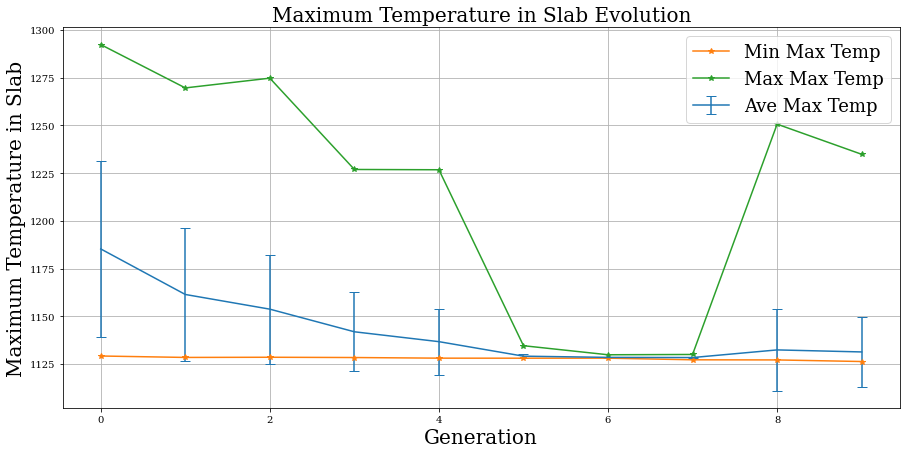
\includegraphics[width=\linewidth]{slab-obj-1-temp-evol.png}
        \caption{Minimum, average, and maximum evolution of AHTR plank's $T_{max}$.}
        \label{fig:slab-obj-1-temp-evol} 
    \end{subfigure}
    \begin{subfigure}{0.9\textwidth}
        \includegraphics[width=\linewidth]{slab-obj-1-temp-final.png}
        \caption{TRISO distribution for the 5 reactor models with the 
        lowest AHTR plank $T_{max}$ at the final generation.}
        \label{fig:slab-obj-1-temp-final} 
    \end{subfigure}
    \begin{subfigure}{0.9\textwidth}
        \includegraphics[width=\linewidth]{slab-obj-1-temp-most-minimized.png}
        \caption{\gls{AHTR} plank model with most-minimized $T_{max}$
        (corresponds to the purple bolded distribution in the above plot).}
        \label{fig:slab-obj-1-temp-most-minimized} 
    \end{subfigure}
    \caption{Simulation p-1b -- ROLLO single-objective optimization to minimize 
    maximum plank temperature ($T_{max}$). Input parameters varied: TRISO 
    packing fraction distribution ($\rho_{TRISO}(\vec{r})$). $PF_{total}$ = 0.0979.}
    \label{fig:slab-obj-1-temp}
\end{figure}

Figure \ref{fig:slab-obj-1-temp-evol} shows that the minimum and average plank's 
$T_{max}$ converged to approximately 1125 K. 
In Figure \ref{fig:slab-obj-1-temp-final}, a mostly flat TRISO packing fraction 
distribution minimizes $T_{max}$ in the plank, the TRISO distribution 
has two small dips at the one-third and two-third points in the plank (6.62cm and 20.48cm). 
A fully flat \gls{TRISO} distribution results in a higher $T_{max}$.
Figure \ref{fig:slab-obj-1-temp-distr} compares the Moltres-generated centerline 
temperature distribution for the plank with mostly flat (Figure 
\ref{fig:slab-obj-1-temp-final}) and flat TRISO distributions for the same 
total packing fraction.
\begin{figure}[htbp!]
    \centering
    \includegraphics[width=\linewidth]{slab-obj-1-temp-distr.png}
    \caption{Comparison of Moltres-generated AHTR plank temperature distribution for 
    non-flat and flat TRISO distribution. 
    Both models have $PF_{total}$ = 0.0979.}
    \label{fig:slab-obj-1-temp-distr}
\end{figure}
The \gls{AHTR} plank with a flat \gls{TRISO} distribution has higher plank temperatures 
on the left and right sides near the moderator. 
To combat this temperature peak, ROLLO found a \gls{TRISO} distribution that 
has a slight dip near the moderator regions, resulting in a lower $T_{max}$.

\subsubsection{Simulation p-1e: Variation of Coolant Channel Shape}
Table \ref{tab:simulationp1e} shows simulation p-1e's optimization problem parameters. 
\begin{table}[htbp!]
    \centering
    \onehalfspacing
    \caption{Simulation p-1e Optimization Problem Parameters}
	\label{tab:simulationp1e}
    \footnotesize
    \begin{tabular}{l|p{3cm}}
    \hline 
    \multicolumn{2}{c}{\textbf{Single Objective: Simulation p-1e}} \\
    \hline 
    \textbf{Objectives} & Minimize $T_{max}$ \\
    \hline 
    \textbf{Input parameter variations} & $0.05<r_{top}<0.35$ \\
    & $0.05<r_{bot}<0.35$ \\
    \hline
    \textbf{Constraints} & $k_{eff} \geq 1.35$\\ 
    & $PF_{total}$ = 0.0979\\
    \hline 
    \textbf{Genetic algorithm parameters} & Population size: 64 \\
    & Generations: 4 \\
    \hline
    \end{tabular}
\end{table}

Figure \ref{fig:slab-obj-1-temp-evol-coolant} shows the plank's $T_{max}$ evolution, 
Figure \ref{fig:slab-obj-1-temp-final-coolant} shows a plot of total radius 
($r_{top} + r_{bot}$) against $T_{max}$, and Figure 
\ref{fig:slab-obj-1-temp-most-minimized-coolant} illustrates the \gls{AHTR} plank model 
with most-minimized $T_{max}$. 
\begin{figure}[htbp!]
    \centering
    \begin{subfigure}{\textwidth}
        \includegraphics[width=\linewidth]{slab-obj-1-temp-evol-coolant.png}
        \caption{Minimum, average, and maximum evolution of AHTR plank's $T_{max}$.}
        \label{fig:slab-obj-1-temp-evol-coolant} 
    \end{subfigure}
    \begin{subfigure}{\textwidth}
        \includegraphics[width=\linewidth]{slab-obj-1-temp-final-coolant.png}
        \caption{Plot of total radius ($r_{top} + r_{bot}$) against plank's 
        $T_{max}$. Red crosses indicate the five reactor models with the 
        lowest $T_{max}$.}
        \label{fig:slab-obj-1-temp-final-coolant} 
    \end{subfigure}
    \begin{subfigure}{\textwidth}
        \includegraphics[width=\linewidth]{slab-obj-1-temp-most-minimized-coolant.png}
        \caption{\gls{AHTR} plank model with most-minimized $T_{max}$. 
        $r_{top} = 0.337$ and $r_{bot} = 0.344$.}
        \label{fig:slab-obj-1-temp-most-minimized-coolant} 
    \end{subfigure}
    \caption{Simulation p-1e -- ROLLO single-objective optimization to minimize 
    maximum plank temperature ($T_{max}$). Input parameters varied: coolant channel shape 
    ($r_{top}, r_{bot}$). $PF_{total}$ = 0.0979.}
    \label{fig:slab-obj-1-temp-coolant}
\end{figure}

Figure \ref{fig:slab-obj-1-temp-final-coolant} demonstrates that there is a negative 
linear correlation between the plank's $T_{max}$ and total radius. 
Comparison of Figures \ref{fig:slab-obj-1-temp-evol} and 
\ref{fig:slab-obj-1-temp-evol-coolant} show that coolant channel shape variation 
does not have as high of an impact on $T_{max}$ as \gls{TRISO} distribution variation:  
the average $T_{max}$ due to \gls{TRISO} variation decreased by 60K over 10 generations, 
while average $T_{max}$ due to coolant channel shape variation only decreased by 15K
over 10 generations. 

\subsection{Objective: Minimize Fuel-Normalized Power Peaking Factor ($PPF_{fuel}$)}
This section reports results from the minimize fuel-normalized power peaking factor 
($PPF_{fuel}$) single-objective optimization simulations: p-1c and p-1f. 
Simulation p-1c varies \gls{TRISO} packing fraction distribution 
($\rho_{TRISO}(\vec{r})$), while simulation p-1f varies the coolant channel shape. 

\subsubsection{Simulation p-1c: Variation of $\rho_{TRISO}(\vec{r})$}
Table \ref{tab:simulationp1c} shows simulation p-1c's optimization problem parameters. 
\begin{table}[htbp!]
    \centering
    \onehalfspacing
    \caption{Simulation p-1c Optimization Problem Parameters}
	\label{tab:simulationp1c}
    \footnotesize
    \begin{tabular}{l|p{3cm}}
    \hline 
    \multicolumn{2}{c}{\textbf{Single Objective: Simulation p-1c}} \\
    \hline 
    \textbf{Objectives} & Minimize $PPF_{fuel}$ \\
    \hline 
    \textbf{Input parameter variations} & $0<a<2$ \\
    & $0<b<\frac{\pi}{2}$ \\
    & $0<c<2\pi$ \\
    \hline
    \textbf{Constraints} & $k_{eff} \geq 1.0$\\ 
    & $PF_{total}$ = 0.0979\\
    \hline 
    \textbf{Genetic algorithm parameters} & Population size: 60 \\
    & Generations: 10 \\
    \hline
    \end{tabular}
\end{table}

Figure \ref{fig:slab-obj-1-ppf-evol} shows the plank's $PPF_{fuel}$ evolution, 
Figure \ref{fig:slab-obj-1-ppf-final} shows the five \gls{TRISO} 
packing fraction distributions ($\rho_{TRISO}(\vec{r})$) in the final generation 
with the most-minimized $PPF_{fuel}$, and Figure 
\ref{fig:slab-obj-1-ppf-most-minimized} illustrates the \gls{AHTR} plank model with 
most-minimized $PPF_{fuel}$. 
\begin{figure}[htbp!]
    \centering
    \begin{subfigure}{0.9\textwidth}
        \includegraphics[width=\linewidth]{slab-obj-1-ppf-evol.png}
        \caption{Minimum, average, and maximum evolution of $PPF_{fuel}$ in the 
        AHTR plank.}
        \label{fig:slab-obj-1-ppf-evol} 
    \end{subfigure}
    \begin{subfigure}{0.9\textwidth}
        \includegraphics[width=\linewidth]{slab-obj-1-ppf-final.png}
        \caption{TRISO distribution for the 5 reactor models with the 
        lowest $PPF_{fuel}$ in AHTR plank at the final generation.}
        \label{fig:slab-obj-1-ppf-final} 
    \end{subfigure}
    \begin{subfigure}{0.9\textwidth}
        \includegraphics[width=\linewidth]{slab-obj-1-ppf-most-minimized.png}
        \caption{\gls{AHTR} plank model with most-minimized $PPF_{fuel}$
        (corresponds to the purple bolded distribution in the above plot).}
        \label{fig:slab-obj-1-ppf-most-minimized} 
    \end{subfigure}
    \caption{Simulation p-1c -- ROLLO single-objective optimization to minimize 
    AHTR plank's fuel-normalized power peaking factor ($PPF_{fuel}$). 
    Input parameters varied: TRISO distribution ($\rho_{TRISO}(\vec{r})$).
    $PF_{total}$ = 0.0979.}
    \label{fig:slab-obj-1-ppf}
\end{figure}

In Figure \ref{fig:slab-obj-1-ppf-final}, the TRISO distribution that best minimizes 
$PPF_{fuel}$ peaks near the edges of the fuel region of the plank, and has a minimum 
point in center of the plank.
This distribution is attributed to \gls{ROLLO} trying to minimize self-shielding effects
in the plank. 
The edges of the fuel region have higher flux as they are closer to the graphite 
moderator, whereas the plank's center has a lower flux due to self shielding. 
The TRISO distribution must follow the flux shape to ensure similar fuel depletion 
rates for different flux regions. 
Thus, to minimize $PPF_{fuel}$, \gls{ROLLO} found a plank 
\gls{TRISO} distribution that has higher packing fraction at the edges, and a 
lower packing fraction in the center. 

\subsubsection{Simulation p-1f: Variation of Coolant Channel Shape}
Table \ref{tab:simulationp1f} shows simulation p-1f's optimization problem parameters. 
\begin{table}[htbp!]
    \centering
    \onehalfspacing
    \caption{Simulation p-1f Optimization Problem Parameters}
	\label{tab:simulationp1f}
    \footnotesize
    \begin{tabular}{l|p{3cm}}
    \hline 
    \multicolumn{2}{c}{\textbf{Single Objective: Simulation p-1f}} \\
    \hline 
    \textbf{Objectives} & Minimize $PPF_{fuel}$ \\
    \hline 
    \textbf{Input parameter variations} & $0.05<r_{top}<0.35$ \\
    & $0.05<r_{bot}<0.35$ \\
    \hline
    \textbf{Constraints} & $k_{eff} \geq 1.35$\\ 
    & $PF_{total}$ = 0.0979\\
    \hline 
    \textbf{Genetic algorithm parameters} & Population size: 64 \\
    & Generations: 5 \\
    \hline
    \end{tabular}
\end{table}

Figure \ref{fig:slab-obj-1-ppf-evol-coolant} shows the plank's $PPF_{fuel}$ evolution 
and Figure \ref{fig:slab-obj-1-ppf-final-coolant} shows a plot of total 
radius ($r_{top} + r_{bot}$) against $PPF_{fuel}$. 
\begin{figure}[htbp!]
    \centering
    \begin{subfigure}{\textwidth}
        \includegraphics[width=\linewidth]{slab-obj-1-ppf-evol-coolant.png}
        \caption{Minimum, average, and maximum evolution of $PPF_{fuel}$ in the 
        AHTR plank.}
        \label{fig:slab-obj-1-ppf-evol-coolant} 
    \end{subfigure}
    \begin{subfigure}{\textwidth}
        \includegraphics[width=\linewidth]{slab-obj-1-ppf-final-coolant.png}
        \caption{Plot of total radius ($r_{top} + r_{bot}$) against $PPF_{fuel}$. 
        Red crosses indicate the five reactor models with the lowest $PPF_{fuel}$.}
        \label{fig:slab-obj-1-ppf-final-coolant} 
    \end{subfigure}
    \caption{Simulation p-1f -- ROLLO single-objective optimization to minimize 
    fuel-normalized power peaking factor ($PPF_{fuel}$) in the slab. 
    Input parameters varied: coolant channel shape ($r_{top}, r_{bot}$). 
    $PF_{total}$ = 0.0979.}
    \label{fig:slab-obj-1-ppf-coolant}
\end{figure}

Comparison of Figures \ref{fig:slab-obj-1-ppf-evol-coolant} and 
\ref{fig:slab-obj-1-ppf-evol} show that coolant channel shape variation 
does not have as high of an impact on $PPF_{fuel}$ as \gls{TRISO} distribution variation:  
the average $PPF_{fuel}$ due to \gls{TRISO} variation decreased by 0.1 over 10 generations, 
while average $PPF_{fuel}$ due to coolant channel shape variation only decreased negligibly
over 10 generations. 
Figure \ref{fig:slab-obj-1-ppf-final-coolant} reiterates that there is no correlation 
between total radius and $PPF_{fuel}$. 

\pagebreak
\section{AHTR Plank: Two-Objective Optimization Results}
In this section, I report the \gls{AHTR} plank's \gls{ROLLO} two-objective 
optimization results. 
The previous section's one-objective optimization results inform the multi-objective 
optimization simulations in this section and Section \ref{sec:plank-three-obj}.
Since the variations in coolant channel shape does not impact two out of three objectives: 
minimize total packing fraction and minimize fuel-normalized power peaking factor 
objectives, I do not conduct two-objective optimization for coolant channel shape 
variations.  
Table \ref{tab:slab-obj-breakdown} summarized the two-objective simulations in this 
section: p-2a, p-2b, and p-2c.

As previously described in Section \ref{sec:opt}, multi-objective optimization returns 
multiple optimal solutions that meet each objective to varying degrees; this set of 
solutions is the Pareto front \cite{deb_multi-objective_2001}. 
For each solution in the Pareto front, none of the objective functions can be 
improved without degrading another objective.
An ideal optimization method for a multi-objective problem like reactor design 
should find widely spread solutions in the obtained Pareto front 
\cite{deb_multi-objective_2001}. 
Thus, I report on the optimal reactor models on the Pareto front for the multi-objective 
optimization problems in this section and Section \ref{sec:plank-three-obj}. 

To ensure that the multi-objective optimization problems are converged, I report the 
hypervolume values for each generation. 
As previously described in Section \ref{sec:binhandkorn}, the hypervolume indicator 
quantifies the Pareto front's goodness (bigger = better).
I use a different reference point for each optimization problem. 
If a multi-objective optimization problem's hypervolume converges earlier than the 
5 generations I intended to run (determined in Section 
\ref{sec:multi-obj-hyperparameters}), I stop running the simulation at that generation. 
However, if the multi-objective optimization problem's hypervolume does not converge by 
generation 5, I run the problem for a few more generations till satisfactory convergence.

\subsection{p-2a: Minimize $PF_{total}$ and $T_{max}$}
\label{sec:p-2a}
This section reports results from the two-objective optimization simulation p-2a, the 
objectives minimized are total fuel packing fraction ($PF_{total}$) and maximum plank
temperature ($T_{max}$).  
Table \ref{tab:simulationp2a} shows simulation p-2a's optimization problem parameters.
\begin{table}[htbp!]
    \centering
    \onehalfspacing
    \caption{Simulation p-2a Optimization Problem Parameters.}
	\label{tab:simulationp2a}
    \footnotesize
    \begin{tabular}{l|p{4cm}}
    \hline 
    \multicolumn{2}{c}{\textbf{Two Objectives: Simulation p-2a}} \\
    \hline 
    \textbf{Objectives} & Minimize $PF_{total}$ \\
    & Minimize $T_{max}$ \\
    \hline 
    \textbf{Input parameter variations} & $0.02<PF_{total}<0.04$ \\
    & $0<a<2$ \\
    & $0<b<\frac{\pi}{2}$ \\
    & $0<c<2\pi$ \\
    \hline
    \textbf{Constraints} & $k_{eff} \geq 1.35$\\ 
    \hline 
    \textbf{Genetic algorithm parameters} & Population size: 128 \\
    & Generations: 2 \\
    \hline
    \end{tabular}
\end{table}

Table \ref{tab:p2a-hypervolume} shows the hypervolume value at each generation, 
confirming that simulation p-2a converges by generation 2. 
\begin{table}[htbp!]
    \centering
    \onehalfspacing
    \caption{Simulation p-2a hypervolume values at each generation.}
	\label{tab:p2a-hypervolume}
    \footnotesize
    \begin{tabular}{ll}
    \hline 
    \multicolumn{2}{c}{\textbf{Two Objectives: Simulation p-2a}} \\
    \multicolumn{2}{c}{Reference point: (0.1, 1350)} \\
    \hline 
    \textbf{Generation} & \textbf{Hypervolume value} \\
    \hline
    1 & 17.659 \\
    2 & 17.659 \\
    \hline
    \end{tabular}
\end{table}

Figure \ref{fig:slab-obj-2-pftemp-pareto} shows a plot of the final generation's reactor 
models' $PF_{total}$ against $T_{max}$, crosses mark the reactor models that 
fall on the Pareto front.
Figure \ref{fig:slab-obj-2-pftemp-pareto-distr} shows the six TRISO distributions in 
the final generation that fall on the Pareto front. 
\begin{figure}[htbp!]
    \centering
    \begin{subfigure}{\textwidth}
        \includegraphics[width=\linewidth]{slab-obj-2-pftemp-pareto.png}
        \caption{Plot of final generation's reactor models' $PF_{total}$ against 
        $T_{max}$. Crosses indicate the reactor models on the Pareto front. 
        Cross colors correspond to TRISO distributions in the plot below.}
        \label{fig:slab-obj-2-pftemp-pareto} 
    \end{subfigure}
    \begin{subfigure}{\textwidth}
        \includegraphics[width=\linewidth]{slab-obj-2-pftemp-pareto-distr.png}
        \caption{TRISO packing fraction distribution for the 6 reactor models on the 
        Pareto front.}
        \label{fig:slab-obj-2-pftemp-pareto-distr} 
    \end{subfigure}
    \caption{Simulation p-2a -- ROLLO two-objective optimization to minimize total 
    fuel packing fraction ($PF_{total}$) and maximum plank temperature ($T_{max}$). 
    Input parameters varied: total fuel packing fraction ($PF_{total}$) and 
    \gls{TRISO} distribution ($\rho_{TRISO}(\vec{r})$).}
    \label{fig:slab-obj-2-pftemp}
\end{figure}
\begin{figure}[htbp!]
    \ContinuedFloat
    \begin{subfigure}{\textwidth}
        \includegraphics[width=\linewidth]{slab-obj-2-pftemp-min-pf.png}
        \caption{\gls{AHTR} plank model with most-minimized $PF_{total}$
        (corresponds to the blue bolded distribution in Figure 
        \ref{fig:slab-obj-2-pftemp-pareto-distr}).}
        \label{fig:slab-obj-2-pftemp-min-pf} 
    \end{subfigure}
    \begin{subfigure}{\textwidth}
        \includegraphics[width=\linewidth]{slab-obj-2-pftemp-min-temp.png}
        \caption{\gls{AHTR} plank model with most-minimized $T_{max}$
        (corresponds to the purple bolded distribution in Figure 
        \ref{fig:slab-obj-2-pftemp-pareto-distr}).}
        \label{fig:slab-obj-2-pftemp-min-temp} 
    \end{subfigure}
    \caption{(contd.) Simulation p-2a -- ROLLO two-objective optimization to minimize 
    total packing fraction ($PF_{total}$) and maximum plank temperature ($T_{max}$). 
    Input parameters varied: total fuel packing fraction ($PF_{total}$) and 
    \gls{TRISO} packing fraction distribution ($\rho_{TRISO}(\vec{r})$).}
\end{figure}

In Figure \ref{fig:slab-obj-2-pftemp-pareto-distr}, the TRISO distribution with the
most-minimized $PF_{total}$ and the highest $T_{max}$ (the blue distribution) has an 
oscillating fuel packing pattern (also illustrated in Figure 
\ref{fig:slab-obj-2-pftemp-min-pf}).
This distribution is similar to simulation p-1a's most-minimized $PF_{total}$ TRISO 
distribution (Figure \ref{fig:slab-obj-1-pf-final}), but differs as it varies between 
0.005 and 0.035, instead of 0 and 0.4, due to influences from the minimize $T_{max}$ 
objective. 
In Figure \ref{fig:slab-obj-2-pftemp-pareto-distr}, the TRISO distribution with the 
most-minimized $T_{max}$ and highest $PF_{total}$ (the purple distribution)
has an almost constant packing fraction of $\sim0.032$ across the plank (also 
illustrated in Figure \ref{fig:slab-obj-2-pftemp-min-temp}). 
This distribution follows a similar flat shape as simulation p-1b's most-minimized 
$T_{max}$ TRISO distribution (Figure \ref{fig:slab-obj-1-temp-final}).

Thus, the \gls{TRISO} distributions on the Pareto front in Figure \ref{fig:slab-obj-2-pftemp} 
that minimizes both $PF_{total}$ and $T_{max}$ have varying degrees of flatness: 
the minimize $T_{max}$ objective influences the flatness and the minimize $PF_{total}$ 
objective influences the oscillating pattern. 

\subsection{p-2b: Minimize $PF_{total}$ and $PPF_{fuel}$}
\label{sec:p-2b}
This section reports results from the two-objective optimization simulation p-2b, the 
objectives minimized are total fuel packing fraction ($PF_{total}$) and fuel-normalized 
power peaking factor ($PPF_{fuel}$).  
Table \ref{tab:simulationp2b} shows simulation p-2b's optimization problem parameters. 
\begin{table}[htbp!]
    \centering
    \onehalfspacing
    \caption{Simulation p-2b Optimization Problem Parameters}
	\label{tab:simulationp2b}
    \footnotesize
    \begin{tabular}{l|p{3cm}}
    \hline 
    \multicolumn{2}{c}{\textbf{Two Objectives: Simulation p-2b}} \\
    \hline 
    \textbf{Objectives} & Minimize $PF_{total}$ \\
    & Minimize $PPF_{fuel}$ \\
    \hline 
    \textbf{Input parameter variations} & $0.02<PF_{total}<0.04$ \\
    & $0<a<2$ \\
    & $0<b<\frac{\pi}{2}$ \\
    & $0<c<2\pi$ \\
    \hline
    \textbf{Constraints} & $k_{eff} \geq 1.35$\\ 
    \hline 
    \textbf{Genetic algorithm parameters} & Population size: 128 \\
    & Generations: 3 \\
    \hline
    \end{tabular}
\end{table}

Table \ref{tab:p2b-hypervolume} shows the hypervolume value at each generation, 
confirming that simulation p-2b converges by generation 3. 
\begin{table}[htbp!]
    \centering
    \onehalfspacing
    \caption{Simulation p-2b hypervolume values at each generation.}
	\label{tab:p2b-hypervolume}
    \footnotesize
    \begin{tabular}{ll}
    \hline 
    \multicolumn{2}{c}{\textbf{Two Objectives: Simulation p-2b}} \\
    \multicolumn{2}{c}{Reference point: (0.1, 1.5)} \\
    \hline 
    \textbf{Generation} & \textbf{Hypervolume value} \\
    \hline
    1 & 0.03607 \\
    2 & 0.03619 \\
    3 & 0.03625 \\
    \hline
    \end{tabular}
\end{table}

Figure \ref{fig:slab-obj-2-pfppf-pareto} shows a plot of the final generation's reactor 
models' $PF_{total}$ against $PPF_{fuel}$, crosses mark the reactor models that fall on 
the Pareto front.
Figure \ref{fig:slab-obj-2-pfppf-pareto-distr} shows the four TRISO packing fraction 
distributions in the final generation that fall on the Pareto front. 
\begin{figure}[htbp!]
    \centering
    \begin{subfigure}{\textwidth}
        \includegraphics[width=\linewidth]{slab-obj-2-pfppf-pareto.png}
        \caption{Plot of final generation's reactor models' $PF_{total}$ against 
        $PPF_{fuel}$. 
        Crosses indicate the reactor models on the Pareto front. Cross colors correspond  
        to TRISO distributions in the plot below.}
        \label{fig:slab-obj-2-pfppf-pareto} 
    \end{subfigure}
    \begin{subfigure}{\textwidth}
        \includegraphics[width=\linewidth]{slab-obj-2-pfppf-pareto-distr.png}
        \caption{TRISO distribution for the 4 reactor models on the Pareto front.}
        \label{fig:slab-obj-2-pfppf-pareto-distr} 
    \end{subfigure}
    \caption{Simulation p-2b -- ROLLO two-objective optimization to minimize total fuel 
    packing fraction ($PF_{total}$) and normalized power peaking factor ($PPF_{fuel}$) 
    in the plank. 
    Input parameters varied: TRISO packing fraction distribution 
    ($\rho_{TRISO}(\vec{r})$).}
    \label{fig:slab-obj-2-pfppf}
\end{figure}
\begin{figure}[htbp!]
    \ContinuedFloat
    \begin{subfigure}{\textwidth}
        \includegraphics[width=\linewidth]{slab-obj-2-pfppf-min-pf.png}
        \caption{\gls{AHTR} plank model with most-minimized $PF_{total}$
        (corresponds to the orange bolded distribution in Figure 
        \ref{fig:slab-obj-2-pfppf-pareto-distr}).}
        \label{fig:slab-obj-2-pfppf-min-pf} 
    \end{subfigure}
    \begin{subfigure}{\textwidth}
        \includegraphics[width=\linewidth]{slab-obj-2-pfppf-min-ppf.png}
        \caption{\gls{AHTR} plank model with most-minimized $PPF_{fuel}$
        (corresponds to the blue bolded distribution in Figure 
        \ref{fig:slab-obj-2-pfppf-pareto-distr}).}
        \label{fig:slab-obj-2-pfppf-min-ppf} 
    \end{subfigure}
    \caption{(contd.) Simulation p-2b -- ROLLO two-objective optimization to minimize 
    total packing fraction ($PF_{total}$) and fuel-normalized power peaking factor 
    ($PPF_{fuel}$) in the plank. 
    Input parameters varied: TRISO packing fraction distribution ($\rho_{TRISO}(\vec{r})$).}
\end{figure}

All reactor models on Figure \ref{fig:slab-obj-2-pfppf}'s Pareto front have a relatively 
flat TRISO packing fraction distribution, varying between 0.02 and 0.04. 
In Figure \ref{fig:slab-obj-2-pfppf-pareto-distr}, the TRISO distribution with the 
most-minimized $PF_{total}$ and highest $PPF_{fuel}$
(the orange distribution) has a constant packing fraction of 0.02 across the plank
(also illustrated in Figure \ref{fig:slab-obj-2-pfppf-min-pf}). 
In Figure \ref{fig:slab-obj-2-pfppf-pareto-distr}, the TRISO distribution with the 
most-minimized $PPF_{fuel}$ and highest $PF_{total}$
(the blue distribution), has a packing fraction that peaks in the center of the plank
and both sides (also illustrated in Figure \ref{fig:slab-obj-2-pfppf-min-ppf}). 
This distribution differs from simulation p-1c's most-minimized $PPF_{fuel}$ TRISO 
distribution (Figure \ref{fig:slab-obj-1-ppf-final}) which has a large $\sim 0.06$ 
variation in TRISO distribution with a minimum point in the center of the plank . 
This difference is due to the different $PF_{total}$ values: simulation p-1c's total PF 
is 0.0979, while the total PF in the most-minimized $PPF_{fuel}$ model 
(blue distribution) is 0.029. 
In Section \ref{sec:p-2b-pf-ppf-study}, I perform a study of $PF_{total}$ 
and $PPF_{fuel}$ to gain a better understand their relationship. 

\subsubsection{Relationship Study: $PF_{total}$ and $PPF_{fuel}$}
\label{sec:p-2b-pf-ppf-study}

\subsection{p-2c: Minimize $T_{max}$ and $PPF_{fuel}$}
\label{sec:p-2c}
This section reports results from the two-objective optimization simulation p-2c, the 
objectives minimized are maximum plank temperature ($T_{max}$) and fuel-normalized 
power peaking factor ($PPF_{fuel}$).  
Table \ref{tab:simulationp2c} shows simulation p-2c's optimization problem parameters. 
\begin{table}[htbp!]
    \centering
    \onehalfspacing
    \caption{Simulation p-2c Optimization Problem Parameters}
	\label{tab:simulationp2c}
    \footnotesize
    \begin{tabular}{l|p{3cm}}
    \hline 
    \multicolumn{2}{c}{\textbf{Two Objectives: Simulation p-2c}} \\
    \hline 
    \textbf{Objectives} & Minimize $T_{max}$ \\
    & Minimize $PPF_{fuel}$ \\
    \hline 
    \textbf{Input parameter variations} & $0<a<2$ \\
    & $0<b<\frac{\pi}{2}$ \\
    & $0<c<2\pi$ \\
    \hline
    \textbf{Constraints} & $k_{eff} \geq 1.0$\\ 
    & $PF_{total}$ = 0.0979\\
    \hline 
    \textbf{Genetic algorithm parameters} & Population size: 120 \\
    & Generations: 3 \\
    \hline
    \end{tabular}
\end{table}

Table \ref{tab:p2c-hypervolume} shows the hypervolume value at each generation, 
confirming that simulation p-2c converges by generation 3. 
\begin{table}[htbp!]
    \centering
    \onehalfspacing
    \caption{Simulation p-2c hypervolume values at each generation.}
	\label{tab:p2c-hypervolume}
    \footnotesize
    \begin{tabular}{ll}
    \hline 
    \multicolumn{2}{c}{\textbf{Two Objectives: Simulation p-2c}} \\
    \multicolumn{2}{c}{Reference point: (1300, 1.6)} \\
    \hline 
    \textbf{Generation} & \textbf{Hypervolume value} \\
    \hline
    1 & 92.041 \\
    2 & 92.087\\
    3 & 92.751 \\
    \hline
    \end{tabular}
\end{table}

Figure \ref{fig:slab-obj-2-tempppf-pareto} shows a plot of the final generation's 
reactor models' $T_{max}$ against $PPF_{fuel}$, crosses mark the reactor models that 
fall on the Pareto front.
Figure \ref{fig:slab-obj-2-tempppf-pareto-distr} shows the eight TRISO distributions in 
the final generation that fall on the Pareto front. 
\begin{figure}[htbp!]
    \centering
    \begin{subfigure}{\textwidth}
        \includegraphics[width=\linewidth]{slab-obj-2-tempppf-pareto.png}
        \caption{Plot of final generation's reactor models' $T_{max}$ against 
        $PPF_{fuel}$. Crosses indicate the reactor models on the Pareto front.
        Cross colors correspond to TRISO distributions in the plot below.}
        \label{fig:slab-obj-2-tempppf-pareto} 
    \end{subfigure}
    \begin{subfigure}{\textwidth}
        \includegraphics[width=\linewidth]{slab-obj-2-tempppf-pareto-distr.png}
        \caption{TRISO packing fraction distribution for the 8 reactor models on the 
        Pareto front.}
        \label{fig:slab-obj-2-tempppf-pareto-distr} 
    \end{subfigure}
    \caption{Simulation p-2c -- ROLLO two-objective optimization to minimize maximum 
    plank temperature ($T_{max}$) and fuel-normalized power peaking factor 
    ($PPF_{fuel}$) in the plank. 
    Input parameters varied: TRISO packing fraction distribution 
    ($\rho_{TRISO}(\vec{r})$). $PF_{total}$ = 0.0979.}
    \label{fig:slab-obj-2-tempppf}
\end{figure}
\begin{figure}[htbp!]
    \ContinuedFloat
    \begin{subfigure}{\textwidth}
        \includegraphics[width=\linewidth]{slab-obj-2-tempppf-min-temp.png}
        \caption{\gls{AHTR} plank model with most-minimized $T_{max}$
        (corresponds to the orange bolded distribution in Figure 
        \ref{fig:slab-obj-2-tempppf-pareto-distr}).}
        \label{fig:slab-obj-2-tempppf-min-temp} 
    \end{subfigure}
    \begin{subfigure}{\textwidth}
        \includegraphics[width=\linewidth]{slab-obj-2-tempppf-min-ppf.png}
        \caption{\gls{AHTR} plank model with most-minimized $PPF_{fuel}$
        (corresponds to the grey bolded distribution in Figure 
        \ref{fig:slab-obj-2-tempppf-pareto-distr}).}
        \label{fig:slab-obj-2-tempppf-min-ppf} 
    \end{subfigure}
    \caption{(contd.) Simulation p-2c -- ROLLO two-objective optimization to minimize 
    maximum plank temperature ($T_{max}$) and fuel-normalized power peaking factor 
    ($PPF_{fuel}$) in the plank. 
    Input parameters varied: TRISO packing fraction distribution 
    ($\rho_{TRISO}(\vec{r})$). $PF_{total}$ = 0.0979.}
\end{figure}

In Figure \ref{fig:slab-obj-2-tempppf-pareto-distr}, the TRISO distribution with 
the most-minimized $T_{max}$ and highest $PPF_{fuel}$ (the orange distribution) 
has an almost constant packing fraction of $\sim0.10$ across the plank, with a 
slight oscillating pattern (also illustrated in Figure 
\ref{fig:slab-obj-2-tempppf-min-temp}).
This distribution follows a similar flat shape as simulation p-1b's most-minimized 
$T_{max}$ TRISO distribution (Figure \ref{fig:slab-obj-1-temp-distr}).
In Figure \ref{fig:slab-obj-2-tempppf-pareto-distr}, the TRISO distribution with 
most-minimized $PPF_{fuel}$ and highest $T_{max}$
(the grey distribution) peaks near the sides of the plank, and has a minimum point at 
the center of the plank (also illustrated in Figure \ref{fig:slab-obj-2-tempppf-min-ppf}). 
This distribution is somewhat similar to p-1c's most-minimized $PPF_{fuel}$ TRISO distribution 
(Figure \ref{fig:slab-obj-1-ppf-final}) which also has a minimum point at the center 
of the plank, but differs as its' peaks are on the fuel regions' edges instead of the 
plank's edges. 

The differences between the above cases and their single objective counterparts in 
Section \ref{sec:plank-one-obj} are due to influences from the other objectives. 

\pagebreak
\section{AHTR Plank: Three-Objective Optimization Results}
\label{sec:plank-three-obj}
In this section, I report the \gls{AHTR} one-third assembly's \gls{ROLLO} three-objective 
optimization results. 
Table \ref{tab:assem-obj-breakdown} summarized the two-objective simulations in this 
section: p-3a, and p-3b. 

\subsection{p-3a: Variation of of $PF_{total}$ and $\rho_{TRISO}(\vec{r})$}
\label{sec:p-3a}
This section reports results from the three-objective optimization simulation p-3a, all 
objectives are minimized: total fuel packing fraction ($PF_{total}$), maximum plank 
temperature ($T_{max}$) and fuel-normalized power peaking factor ($PPF_{fuel}$).  
The input parameters varied are total fuel packing fraction ($PF_{total}$) and 
TRISO packing fraction distribution ($\rho_{TRISO}(\vec{r})$). 
Table \ref{tab:simulationp3a} shows simulation p-3a's optimization problem parameters. 
\begin{table}[htbp!]
    \centering
    \onehalfspacing
    \caption{Simulation p-3a Optimization Problem Parameters}
	\label{tab:simulationp3a}
    \footnotesize
    \begin{tabular}{l|p{4cm}}
    \hline 
    \multicolumn{2}{c}{\textbf{Three Objectives: Simulation p-3a}} \\
    \hline 
    \textbf{Objectives} & Minimize $PF_{total}$ \\
    & Minimize $T_{max}$ \\
    & Minimize $PPF_{fuel}$ \\
    \hline 
    \textbf{Input parameter variations} & $0.02<PF_{total}<0.04$ \\
    & $0<a<2$ \\
    & $0<b<\frac{\pi}{2}$ \\
    & $0<c<2\pi$ \\
    \hline
    \textbf{Constraints} & $k_{eff} \geq 1.35$\\ 
    \hline 
    \textbf{Genetic algorithm parameters} & Population size: 128 \\
    & Generations: 5 \\
    \hline
    \end{tabular}
\end{table}

Table \ref{tab:p3a-hypervolume} shows the hypervolume value at each generation, 
confirming that simulation p-3a converges by generation 5. 
\begin{table}[htbp!]
    \centering
    \onehalfspacing
    \caption{Simulation p-3a hypervolume values at each generation.}
	\label{tab:p3a-hypervolume}
    \footnotesize
    \begin{tabular}{ll}
    \hline 
    \multicolumn{2}{c}{\textbf{Three Objectives: Simulation p-3a}} \\
    \multicolumn{2}{c}{Reference point: (0.06, 1260 ,1.5)} \\
    \hline 
    \textbf{Generation} & \textbf{Hypervolume value} \\
    \hline
    1 & 2.392 \\
    2 & 2.392 \\
    3 & 2.393 \\
    4 & 2.442 \\
    5 & 2.446 \\
    \hline
    \end{tabular}
\end{table}

Figure \ref{fig:slab-obj-3-3d} shows a 3D plot of the final generation's reactor models' 
$PF_{total}$ against $T_{max}$ against $PPF_{fuel}$, crosses mark the reactor models 
that fall on the Pareto front.
Figure \ref{fig:slab-obj-3-distr} shows the 14 TRISO packing fraction distributions in 
the final generation that fall on the Pareto front. 
\begin{figure}[htbp!]
    \begin{subfigure}{\textwidth}
        \centering
        \includegraphics[width=0.7\linewidth]{slab-obj-3-3d.png}
        \caption{Plot of final generation's reactor models' $PF_{total}$ against 
        $T_{max}$ against $PPF_{fuel}$. Crosses indicate the reactor models on the 
        Pareto front. Cross colors correspond to TRISO distributions in the plot below.}
        \label{fig:slab-obj-3-3d} 
    \end{subfigure}
    \begin{subfigure}{\textwidth}
        \includegraphics[width=\linewidth]{slab-obj-3-distr.png}
        \caption{TRISO packing fraction distribution for the 14 reactor models on the Pareto front.}
        \label{fig:slab-obj-3-distr} 
    \end{subfigure}
    \caption{Simulation p-3a -- ROLLO three-objective optimization to minimize total 
    fuel packing fraction ($PF_{total}$), maximum plank temperature ($T_{max}$) and 
    fuel-normalized power peaking factor ($PPF_{fuel}$) in the plank. 
    Input parameters varied: $PF_{total}$, TRISO packing fraction distribution
    ($\rho_{TRISO}(\vec{r})$).}
    \label{fig:slab-obj-3}
\end{figure}

Figure \ref{fig:slab-obj-3-3d} demonstrates that \gls{ROLLO} found 14 widely spread 
solutions in the final generation's Pareto front. 
Figure \ref{fig:slab-obj-3-distr} demonstrates that the TRISO distributions on the
Pareto front have maximum packing fraction variation of $\sim0.01$. 
Figure \ref{fig:slab-obj-3-distr-most-minimized} shows the three distributions from 
Figure \ref{fig:slab-obj-3-distr} that most-minimized each objective. 
\begin{figure}[htbp!]
    \centering
    \begin{subfigure}{\textwidth}
        \includegraphics[width=\linewidth]{slab-obj-3-distr-most-minimized.png}
        \caption{TRISO distribution for the 3 reactor models on the Pareto front
        that most minimized each objective.}
        \label{fig:slab-obj-3-distr-most-minimized}
    \end{subfigure}
    \begin{subfigure}{0.8\textwidth}
        \includegraphics[width=\linewidth]{slab-obj-3-min-pf.png}
        \caption{\gls{AHTR} plank model with most-minimized $PF_{total}$ 
        (corresponds to the purple distribution in the above plot).}
        \label{fig:slab-obj-3-min-pf} 
    \end{subfigure}
    \begin{subfigure}{0.8\textwidth}
        \includegraphics[width=\linewidth]{slab-obj-3-min-temp.png}
        \caption{\gls{AHTR} plank model with most-minimized $T_{max}$
        (corresponds to the orange distribution in the above plot).}
        \label{fig:slab-obj-3-min-temp} 
    \end{subfigure}
    \begin{subfigure}{0.8\textwidth}
        \includegraphics[width=\linewidth]{slab-obj-3-min-ppf.png}
        \caption{\gls{AHTR} plank model with most-minimized $PPF_{fuel}$
        (corresponds to the pink distribution in the above plot).}
        \label{fig:slab-obj-3-min-ppf} 
    \end{subfigure}
    \caption{AHTR models and TRISO distribution for the 3 reactor models on simulation 
    p-3a's Pareto front that most-minimized each objective.
    Simulation p-3a -- ROLLO three-objective optimization to minimize total fuel packing 
    fraction ($PF_{total}$), maximum plank temperature ($T_{max}$) and 
    normalized power peaking factor ($PPF_{fuel}$) in the plank. 
    Input parameters varied: $PF_{total}$, TRISO packing fraction distribution
    ($\rho_{TRISO}(\vec{r})$)}
    \label{fig:slab-obj-3-most-minimized}
\end{figure}

In Figure \ref{fig:slab-obj-3-distr-most-minimized}, the TRISO distribution with the
most-minimized $PF_{total}$ (the purple distribution) has an oscillating fuel 
packing pattern (also illustrated in Figure \ref{fig:slab-obj-3-min-pf}).
This distribution is similar to simulation p-1a's most-minimized $PF_{total}$ TRISO 
distribution (Figure \ref{fig:slab-obj-1-pf-final}) with its oscillating fuel pattern. 
In Figure \ref{fig:slab-obj-3-distr-most-minimized}, the TRISO distribution with the 
most-minimized $T_{max}$ (the orange distribution) has mostly flat TRISO distribution 
(also illustrated in Figure \ref{fig:slab-obj-3-min-temp}). 
This distribution follows a similar distribution as simulation p-1b's most-minimized 
$T_{max}$ TRISO distribution (Figure \ref{fig:slab-obj-1-temp-final}): a mostly flat 
TRISO distribution with two small dips at the one-third and two-third points in the 
plank.
In Figure \ref{fig:slab-obj-3-distr-most-minimized}, the TRISO distribution with the
most-minimized $PPF_{fuel}$ (the pink distribution) has a 
slightly oscillating fuel packing pattern (also illustrated in Figure 
\ref{fig:slab-obj-3-min-ppf}).

Most of the \gls{TRISO} distributions on the Pareto front (Figure 
\ref{fig:slab-obj-3-distr}) have a mostly flat distribution with approximately 
$\sim0.1cm$ of variation. 
The flatness is influenced by the minimize $T_{max}$ objective. 
As observed in previous sections \ref{sec:plank-1-obj-temp}, \ref{sec:p-2a}, and 
\ref{sec:p-2c}, a flat \gls{TRISO} distribution minimizes $T_{max}$ objective.
The variations in \gls{TRISO} distributions are influenced by both the minimize 
total packing fraction and minimize $PPF_{fuel}$ objectives. 
The minimize total packing fraction objective tries to minimize self shielding effects 
to enable a higher $k_{eff}$ for lower total PF. 
The fuel-normalized power peaking factor objective tries to minimize 
TRISO fuel in areas with higher flux to minimize fuel-normalized power peaking.

Section \ref{sec:plank-discussion} further discusses \gls{ROLLO}'s plank 
optimization results and significance for reactor designers.

\subsection{p-3b: Variation of $PF_{total}$, $\rho_{TRISO}(\vec{r})$, and Coolant 
Channel Shape}
This section reports results from the three-objective optimization simulation p-3b, 
all objectives are minimized: total fuel packing fraction ($PF_{total}$), maximum plank 
temperature ($T_{max}$) and fuel-normalized power peaking factor ($PPF_{fuel}$).  
The input parameters varied are total fuel packing fraction ($PF_{total}$), 
TRISO packing fraction distribution ($\rho_{TRISO}(\vec{r})$), and coolant channel 
shape.  
Table \ref{tab:simulationp3b} shows simulation p-3b's optimization problem parameters. 
\begin{table}[htbp!]
    \centering
    \onehalfspacing
    \caption{Simulation p-3b Optimization Problem Parameters}
	\label{tab:simulationp3b}
    \footnotesize
    \begin{tabular}{l|p{4cm}}
    \hline 
    \multicolumn{2}{c}{\textbf{Three Objectives: Simulation p-3b}} \\
    \hline 
    \textbf{Objectives} & Minimize $PF_{total}$ \\
    & Minimize $T_{max}$ \\
    & Minimize $PPF_{fuel}$ \\
    \hline 
    \textbf{Input parameter variations} & $0.02<PF_{total}<0.04$ \\
    & $0<a<2$ \\
    & $0<b<\frac{\pi}{2}$ \\
    & $0<c<2\pi$ \\
    & $0.05<r_{top}<0.35$ \\
    & $0.05<r_{bot}<0.35$ \\
    \hline
    \textbf{Constraints} & $k_{eff} \geq 1.35$\\ 
    \hline 
    \textbf{Genetic algorithm parameters} & Population size: 128 \\
    & Generations: 8 \\
    \hline
    \end{tabular}
\end{table}

Table \ref{tab:p3b-hypervolume} shows the hypervolume value at each generation, 
confirming that simulation p-3b converges by generation 8. 
\begin{table}[htbp!]
    \centering
    \onehalfspacing
    \caption{Simulation p-3b hypervolume values at each generation.}
	\label{tab:p3b-hypervolume}
    \footnotesize
    \begin{tabular}{ll}
    \hline 
    \multicolumn{2}{c}{\textbf{Three Objectives: Simulation p-3b}} \\
    \multicolumn{2}{c}{Reference point: (0.06, 1260 ,1.5)} \\
    \hline 
    \textbf{Generation} & \textbf{Hypervolume value} \\
    \hline
    1 & 1.985 \\
    2 & 2.119 \\
    3 & 2.158 \\
    4 & 2.251\\
    5 & 2.262 \\
    6 & 2.280 \\
    7 & 2.310 \\
    8 & 2.313 \\
    \hline
    \end{tabular}
\end{table}

Figure \ref{fig:slab-obj-3-3d-all} shows a 3D plot of the final generation's reactor 
models' $PF_{total}$ against $T_{max}$ against $PPF_{fuel}$, crosses mark the 
reactor models that fall on the Pareto front.
Figure \ref{fig:slab-obj-3-distr-all} shows the 21 TRISO distributions and their
total radius $(r_{top}, r_{bot})$ in the final generation that fall on the Pareto 
front. 
\begin{figure}[htbp!]
    \begin{subfigure}{\textwidth}
        \centering
        \includegraphics[width=0.7\linewidth]{slab-obj-3-3d-all.png}
        \caption{Plot of final generation's reactor models' $PF_{total}$ against 
        $T_{max}$ against $PPF_{fuel}$. Crosses indicate the reactor models on the 
        Pareto front. Cross colors correspond to TRISO distributions in the plot below.}
        \label{fig:slab-obj-3-3d-all} 
    \end{subfigure}
    \begin{subfigure}{\textwidth}
        \includegraphics[width=\linewidth]{slab-obj-3-distr-all.png}
        \caption{TRISO distribution for the 21 reactor models on the Pareto front.}
        \label{fig:slab-obj-3-distr-all} 
    \end{subfigure}
    \caption{Simulation p-3b -- ROLLO three-objective optimization to minimize total 
    fuel packing fraction ($PF_{total}$), maximum plank temperature ($T_{max}$), and 
    fuel-normalized power peaking factor ($PPF_{fuel}$) in the plank. 
    Input parameters varied: total fuel packing fraction $PF_{total}$, 
    TRISO packing fraction distribution ($\rho_{TRISO}(\vec{r})$), 
    coolant channel shape $(r_{top}, r_{bot})$.}
    \label{fig:slab-obj-3-all}
\end{figure}

Figure \ref{fig:slab-obj-3-3d-all} demonstrates that \gls{ROLLO} found 21 widely spread 
solutions in the final generation's Pareto front. 
Figure \ref{fig:slab-obj-3-distr-most-minimized-distr-all} shows the three distributions 
from Figure \ref{fig:slab-obj-3-distr-all} that most-minimized each objective. 
Figures \ref{fig:slab-obj-3-all-min-pf}, \ref{fig:slab-obj-3-all-min-temp}, and 
\ref{fig:slab-obj-3-all-min-ppf} show the \gls{AHTR} plank's TRISO distribution and 
coolant channel shape for most-minimized cases. 
\begin{figure}[htbp!]
    \begin{subfigure}{\textwidth}
        \includegraphics[width=\linewidth]{slab-obj-3-distr-most-minimized-all.png}
        \caption{TRISO distribution for the 3 reactor models on the Pareto 
        front that most minimized each objective.}
        \label{fig:slab-obj-3-distr-most-minimized-distr-all}
    \end{subfigure}
    \begin{subfigure}{\textwidth}
        \includegraphics[width=\linewidth]{slab-obj-3-all-min-pf.png}
        \caption{TRISO distribution and coolant channel shape that most-minimized 
        $PF_{total}$ (corresponds to the red distribution in the above plot).}
        \label{fig:slab-obj-3-all-min-pf}
    \end{subfigure}
    \begin{subfigure}{\textwidth}
        \includegraphics[width=\linewidth]{slab-obj-3-all-min-tempppf.png}
        \caption{TRISO distribution and coolant channel shape that most minimized 
        $T_{max}$ (corresponds to the pink distribution in the above plot).}
        \label{fig:slab-obj-3-all-min-temp}
    \end{subfigure}
    \begin{subfigure}{\textwidth}
        \includegraphics[width=\linewidth]{slab-obj-3-all-min-tempppf.png}
        \caption{TRISO distribution and coolant channel shape that most minimized 
        $PPF_{fuel}$ (corresponds to the pink distribution in the above plot).}
        \label{fig:slab-obj-3-all-min-ppf}
    \end{subfigure}
    \caption{AHTR models and TRISO distribution for the 3 reactor models on simulation 
    p-3b -- ROLLO three-objective optimization to minimize total 
    fuel packing fraction ($PF_{total}$), maximum plank temperature ($T_{max}$), and 
    fuel-normalized power peaking factor ($PPF_{fuel}$) in the plank. 
    Input parameters varied: total fuel packing fraction $PF_{total}$, 
    TRISO packing fraction distribution ($\rho_{TRISO}(\vec{r})$), 
    coolant channel shape $(r_{top}, r_{bot})$.}
    \label{fig:slab-obj-3-distr-most-minimized-all}
\end{figure}

In Figure \ref{fig:slab-obj-3-distr-most-minimized-distr-all}, the \gls{AHTR} plank model 
with the most-minimized $PF_{total}$ (the pink distribution) has a oscillating fuel 
packing pattern with approximately $\sim0.2cm$ of variation and total coolant channel radius 
of 0.399cm (illustrated in Figure \ref{fig:slab-obj-3-all-min-pf}).
In Figure \ref{fig:slab-obj-3-distr-most-minimized-distr-all}, the \gls{AHTR} plank model with 
the most-minimized $T_{max}$ and $PPF_{fuel}$ (the red distribution) 
has a flat TRISO distribution and total coolant channel radius of 0.657cm 
(illustrated in Figure \ref{fig:slab-obj-3-all-min-tempppf}). 

Similar to simulation p-3a (Section \ref{sec:p-3a}), most of the \gls{TRISO} distributions 
on the Pareto front have a mostly flat distribution with maximum $\sim0.1cm$ of 
variation. 
The flatness is influenced by the minimize $T_{max}$ objective. 
As observed in previous sections \ref{sec:plank-1-obj-temp}, \ref{sec:p-2a}, and 
\ref{sec:p-2c}, a flat \gls{TRISO} distribution minimizes $T_{max}$ objective.
The variations in \gls{TRISO} distributions are influenced by both the minimize 
$PF_{total}$ and minimize $PPF_{fuel}$ objectives. 
The minimize total packing fraction objective tries to minimize self shielding effects 
to enable a higher $k_{eff}$ for lower total PF. 
The minimize fuel-normalized power peaking factor objective tries to minimize 
TRISO distribution in areas with higher flux to minimize fuel-normalized power peaking.
% talk about coolant channel shape influences T_max. but not as much 
% the other objectives are not impacted by coolant channel shape. 

Section \ref{sec:plank-discussion} further discusses \gls{ROLLO}'s plank 
optimization results and significance for reactor designers.

\pagebreak
\section{AHTR Plank: Computational Cost Summary}
\label{sec:plank-compute-cost}
Optimization simulations are run on the BlueWaters supercomputer \cite{ncsa_about_2017} and
the Theta supercomputer at the Argonne Leadership Computing Facility under the Director's 
Discretionary Allocation Program \cite{noauthor_argonne_2022}. 
Each BlueWaters compute node has 32 processor cores with a nominal clock speed of 3.2GHz
\cite{ncsa_about_2017}, and each Theta compute node has 64 processor cores with a nominal 
clock speed of 1.5GHz \cite{noauthor_argonne_2022}.  

Each optimization simulation takes a different amount of node-hours to run due to 
differences in simulation software, tallies and intermediate steps required. 
Table \ref{tab:plank-compute-cost} reports the computational cost for each optimization 
simulation. 
Table \ref{tab:slab-obj-breakdown} detailed the simulation parameters.
\begin{table}[htbp!]
    \centering
    \onehalfspacing
    \caption{Computational cost of \acrfull{ROLLO} simulations for optimizing \acrfull{AHTR}
    plank. BW: BlueWaters Supercomputer, Theta: Theta supercomputer.}
	\label{tab:plank-compute-cost}
    \footnotesize
    \begin{tabular}{p{1.4cm}|p{1cm}lp{4cm}lp{4cm}}
    \hline 
    \textbf{Num of Objs} & \textbf{Sim} & \textbf{Machine} & \textbf{Compute cost per gen [node-hours]} &\textbf{gens} & \textbf{Total compute cost [node-hours]} \\
    \hline
    \multirow{6}{2cm}{1} 
    & p-1a & BW & 23.9 & 10 & 238.7 \\
    & p-1b & BW & 96.0 & 10 & 959.7 \\
    & p-1c & BW & 65.9 & 10 & 658.6 \\
    & p-1d & Theta & 49.6 & 3 & 148.7 \\
    & p-1e & Theta & 71.4 & 4 & 285.6 \\
    & p-1f & Theta & 46.4 & 5 & 231.8 \\
    \hline
    \multirow{3}{2cm}{2}
    & p-2a & Theta & 132.2 & 2 & 264.5 \\
    & p-2b & Theta & 66.3 & 3 & 198.9 \\
    & p-2c & Theta & 167.1 & 3 & 501.2 \\
    \hline
    \multirow{2}{2cm}{3}
    & p-3a & Theta & 92.9 & 5 & 464.5 \\
    & p-3b & Theta & 181.2 & 5 & 906.2 \\
    \hline
    \end{tabular}
\end{table}

\section{AHTR Plank Optimization Results Discussion and Significance}
\label{sec:plank-discussion}
\gls{ROLLO} successfully finds widely spread solutions in each of the multi-objective 
optimization final generation's Pareto front.
\gls{ROLLO} is a global search of a large design space and helps narrow down possible 
solutions.
This informs reactor designers of optimal reactor parameters for their defined objectives.  
From here, reactor designers can conduct sensitivity analysis and use high fidelity 
models to characterize a smaller section of the design space.

\section{Summary}
%\chapter{AHTR One-Third Assembly Optimization Results}
\glsresetall
\label{chap:ahtr-assem-opt-results}
In this chapter, I report the \gls{AHTR} one-third assembly's \gls{ROLLO} optimization 
results. 
I vary the following \gls{AHTR} one-third assembly input parameters:
\begin{itemize}
    \item \gls{TRISO} packing fraction distribution ($\rho_{TRISO}(\vec{r})$)
    \item Total fuel packing fraction ($PF_{total}$)
    \item Coolant channel shape ($r_1, r_2, r_3, r_4,$ and $r_5$)
\end{itemize} 
Section \ref{sec:input-parameter-modeling} detailed how I vary these 
\gls{AHTR} one-third assembly's input parameters. 
I optimize the \gls{AHTR} one-third assembly for the following 
objectives:
\begin{itemize}
    \item Minimize total fuel packing fraction ($PF_{total}$)
    \item Minimize maximum one-third assembly temperature ($T_{max}$)
    \item Minimize fuel-normalized power peaking factor ($PPF_{fuel}$)
\end{itemize} 
Table \ref{tab:objectives} outlined these objectives and their motivation.
Chapter \ref{chap:method} detailed the methodology for \gls{AHTR} one-third 
assembly modeling and \gls{ROLLO} optimization. 

The subsequent sections outline the \gls{AHTR} one-third assembly's optimization 
simulations, describe the single-objective and multi-objective \gls{ROLLO} optimization 
simulations' results, report each simulation's computational cost, and discuss the 
results' significance.

\section{ROLLO AHTR One-Third Assembly Optimization Simulations Overview}
Table \ref{tab:assem-obj-breakdown} shows the details of the \gls{ROLLO} 
optimization problems explored in this chapter.
\begin{table}[htbp!]
    \centering
    \onehalfspacing
    \caption{\acrfull{ROLLO} simulations for optimizing \acrfull{AHTR}
    one-third assembly. $PF_{total}$: Total Fuel Packing Fraction, 
    $T_{max}$: Maximum one-third assembly Temperature, 
    $PPF_{fuel}$: Normalized Power Peaking Factor, $\rho_{TRISO}(\vec{r})$: 
    \gls{TRISO} packing fraction distribution}
	\label{tab:assem-obj-breakdown}
    \footnotesize
    \begin{tabular}{p{1.4cm}|p{1cm}|lllp{3cm}}
    \hline 
    \textbf{Num of Objs} & \textbf{Sim} & \textbf{Objectives} & \textbf{Constraints} &\textbf{Varying Parameters} & \textbf{Coupled Nuclear Software} \\
    \hline
    \multirow{9}{2cm}{1}& a-1a & \tabitem min($PF_{total}$) & \tabitem $k_{eff} \geq 1.38$ &\tabitem $\rho_{TRISO}(\vec{r})$ & OpenMC \\
    & & & & \tabitem $PF_{total}$ & \\
    \cline{2-6}
    & a-1b & \tabitem min($T_{max}$) & \tabitem $k_{eff} \geq 1.38$ &\tabitem $\rho_{TRISO}(\vec{r})$ & OpenMC, Moltres\\
    \cline{2-6}
    & a-1c & \tabitem min($PPF_{fuel}$) & \tabitem $k_{eff} \geq 1.38$ &\tabitem $\rho_{TRISO}(\vec{r})$ & OpenMC\\
    \cline{2-6}
    & a-1d & \tabitem min($PF_{total}$) & \tabitem $k_{eff} \geq 1.0$ &\tabitem Coolant channel shape & OpenMC \\
    & & & & \tabitem $PF_{total}$ & \\
    \cline{2-6}
    & a-1e & \tabitem min($T_{max}$) & \tabitem $k_{eff} \geq 1.38$ &\tabitem Coolant channel shape & OpenMC, Moltres\\
    \cline{2-6}
    & a-1f & \tabitem min($PPF_{fuel}$) & \tabitem $k_{eff} \geq 1.0$ &\tabitem Coolant channel shape & OpenMC\\
    \hline
    \multirow{6}{2cm}{2}& a-2a & \tabitem min($PF_{total}$) & \tabitem $k_{eff} \geq 1.38$ & \tabitem $\rho_{TRISO}(\vec{r})$ & OpenMC, Moltres\\
    & &\tabitem min($T_{max}$) & & \tabitem $PF_{total}$ & \\
    \cline{2-6}
    & a-2b & \tabitem min($PF_{total}$) & \tabitem $k_{eff} \geq 1.38$ & \tabitem $\rho_{TRISO}(\vec{r})$ & OpenMC\\
    & & \tabitem min($PPF_{fuel}$) & & \tabitem $PF_{total}$ & \\
    \cline{2-6}
    & a-2c & \tabitem min($T_{max}$) & \tabitem $k_{eff} \geq 1.38$ & \tabitem $\rho_{TRISO}(\vec{r})$ & OpenMC, Moltres\\
    & & \tabitem min($PPF_{fuel}$) & & & \\
    \hline
    \multirow{6}{2cm}{3}& a-3a &\tabitem min($PF_{total}$) & \tabitem $k_{eff} \geq 1.38$ & \tabitem $\rho_{TRISO}(\vec{r})$ & OpenMC, Moltres\\
    && \tabitem min($PPF_{fuel}$) & & \tabitem $PF_{total}$ & \\
    && \tabitem min($T_{max}$) & & & \\
    \cline{2-6}
    & a-3b &\tabitem min($PF_{total}$) & \tabitem $k_{eff} \geq 1.38$ & \tabitem $\rho_{TRISO}(\vec{r})$ & OpenMC, Moltres\\
    && \tabitem min($PPF_{fuel}$) & & \tabitem $PF_{total}$ & \\
    && \tabitem min($T_{max}$) & & \tabitem Coolant channel shape& \\
    \hline
    \end{tabular}
\end{table}
I first conducted single objective, single input parameter \gls{ROLLO} optimizations 
to understand the individual impacts of each objective on each input parameter. 
Their results will inform the multi-objective optimization simulations setup. 
% TODO: update the keff constraint in table
% explain why some simulations use keff > 1.0 and that I didn't rerun because 
% I expect the same correlation results. 

Simulations are run on the Theta supercomputer at the Argonne Leadership Computing 
Facility under the Director's Discretionary Allocation Program 
\cite{noauthor_argonne_2022}. 
Section \ref{sec:assem-compute-cost} details each optimization simulation's computational 
cost.  

\section{AHTR One-Third Assembly: Single-Objective Optimization Results}
\label{sec:assem-one-obj}
This section reports the \gls{AHTR} one-third assembly's \gls{ROLLO} 
single-objective optimization results. 
Table \ref{tab:assem-obj-breakdown} summarized the one-objective simulations:
a-1a, a-1b, a-1c, a-1d, a-1e, and a-1f. 
In the following subsections, I describe the single-objective optimization results 
grouped by the minimized objective. 

If a single-objective optimization problem's objective converges earlier than the 
5 generations I intended to run (determined in Section 
\ref{sec:multi-obj-hyperparameters}), I stop the simulation at that generation. 
Section \ref{sec:rollo-convergence} described how reactor designers use 
\gls{ROLLO} to determine problem convergence. 

\subsection{Objective: Minimize Total Packing Fraction ($PF_{total}$)}
\label{sec:assem-1-obj-pf}
This section reports results from the minimize total fuel packing fraction 
($PF_{total}$) single-objective optimization simulations: a-1a and a-1d. 
Simulation a-1a varies the $PF_{total}$ and \gls{TRISO} 
packing fraction distribution ($\rho_{TRISO}(\vec{r})$), and simulation a-1d varies 
the $PF_{total}$ and coolant channel shape ($r_1, r_2, r_3, r_4,$ and $r_5$). 

\subsubsection{Simulation a-1a: Variation of $PF_{total}$ and $\rho_{TRISO}(\vec{r})$}
Table \ref{tab:simulationa1a} shows simulation a-1a's optimization problem parameters. 
\begin{table}[htbp!]
    \centering
    \onehalfspacing
    \caption{Simulation a-1a Optimization Problem Parameters}
	\label{tab:simulationa1a}
    \footnotesize
    \begin{tabular}{l|p{5.3cm}}
    \hline 
    \multicolumn{2}{c}{\textbf{Single Objective: Simulation a-1a}} \\
    \hline 
    \textbf{Objectives} & Minimize $PF_{total}$ \\
    \hline 
    \textbf{Input Parameter Variations} & $0.05<PF_{total}<0.07$ \\
    & $\rho_{TRISO}(\vec{r})$: $0<a<2$, $0<d<2$\\
    & $\rho_{TRISO}(\vec{r})$: $0<b<\frac{\pi}{2}$, $0<e<\frac{\pi}{2}$\\
    & $\rho_{TRISO}(\vec{r})$: $0<c<2\pi$, $0<f<2\pi$\\
    \hline
    \textbf{Constraints} & $k_{eff} \geq 1.38$\\ 
    \hline 
    \textbf{Genetic Algorithm Parameters} & Population size: 128 \\
    & Generations: 3 \\
    \hline
    \end{tabular}
\end{table}

The one-third assembly's TRISO distribution is varied based on sine distributions, 
as described in Section \ref{sec:input-parameter-modeling}. 
If the simulation used the FHR benchmark equivalent $PF_{total} = 0.153$, at
certain sine distributions, some fuel cells will have $PF > 0.3$. 
OpenMC's random sequential packing algorithm becomes prohibitively slow at $PF > 0.3$, 
resulting in long runtimes. 
Therefore, I used $PF_{total} = 0.06$ because it is approximately the smallest 
$PF_{total}$ that enables $k_{eff} \geq 1.38$ and will avoid fuel cells with 
$PF > 0.3$ occurences. 
I use $PF_{total} = 0.06$ for all optimization simulations that do not vary 
$PF_{total}$: a-1b, a-1c, a-1e, a-1f, and a-2c. 
And I vary $PF_{total}$ between $0.05$ and $0.07$ for all optimization simulations 
that do vary $PF_{total}$: a-1a, a-1d, a-2a, a-2b, a-3a, and a-3b.

Figure \ref{fig:assem-obj-1-pf-evol} shows the $PF_{total}$ evolution.
Figure \ref{fig:assem-obj-1-pf-final} shows four unique TRISO packing fraction 
distributions in the final generation with the most-minimized $PF_{total}$. 
Figure \ref{fig:assem-obj-1-pf-most-minimized} illustrates the \gls{AHTR} one-third 
assembly model with the most-minimized $PF_{total}$.
\begin{figure}[htbp!]
    \begin{subfigure}{\textwidth}
        \centering
        \includegraphics[width=\linewidth]{assem-obj-1-pf-evol.png}
        \caption{Minimum, average, and maximum $PF_{total}$ evolution.}
        \label{fig:assem-obj-1-pf-evol} 
    \end{subfigure}
    \begin{subfigure}{\textwidth}
        \centering
        \includegraphics[width=\linewidth]{assem-obj-1-pf-final.png}
        \caption{TRISO packing fraction distribution for four unique reactor models with the 
        smallest $PF_{total}$ in the final generation.}
        \label{fig:assem-obj-1-pf-final} 
    \end{subfigure}
    \caption{Simulation a-1a -- ROLLO single-objective optimization to minimize total 
    fuel packing fraction ($PF_{total}$) in \gls{AHTR} one-third assembly. 
    Input parameters varied: $PF_{total}$, \gls{TRISO} packing fraction 
    distribution ($\rho_{TRISO}(\vec{r})$).}
    \label{fig:assem-obj-1-pf}
\end{figure}
\begin{figure}[htbp!]
    \ContinuedFloat
    \begin{subfigure}{\textwidth}
        \centering
        \includegraphics[width=0.7\linewidth]{assem-obj-1-pf-most-minimized.png}
        \caption{\gls{AHTR} one-third assembly model with the most-minimized 
        $PF_{total}$, corresponding to the the first TRISO distribution in Figure 
        \ref{fig:assem-obj-1-pf-final}. The reactor model has $PF_{total}=0.0559$
        and $k_{eff}=1.3802$.}
        \label{fig:assem-obj-1-pf-most-minimized} 
    \end{subfigure}
    \caption{(contd.) Simulation a-1a -- ROLLO single-objective optimization to minimize total 
    fuel packing fraction ($PF_{total}$) in \gls{AHTR} one-third assembly. 
    Input parameters varied: total fuel packing fraction 
    ($PF_{total}$), \gls{TRISO} packing fraction distribution ($\rho_{TRISO}(\vec{r})$).}
\end{figure}

Figure \ref{fig:assem-obj-1-pf-evol} shows that the minimum and average $PF_{total}$ 
converged to approximately 0.057 in the final generation. 
In Figure \ref{fig:assem-obj-1-pf-final}, the four unique TRISO packing fraction 
distributions in the final generation that most-minimized $PF_{total}$ have various 
oscillating TRISO distribution patterns. 

The one-third assembly model with the most-minimized $PF_{total}$ has a 
$PF_{total} =0.0559$, an oscillating TRISO distribution along the both the 
x-axis and y-axis, and a packing fraction standard deviation of $0.04$ across the 
one-third assembly. 
Along the x-axis, the distribution peaks on the even fuel cell columns (at 8.2cm, 12.3cm, 
16.4cm, 20.5cm, and 24.5cm). 
The even columns have the largest y-axis variation of $\sim0.05$ with peaks of
$PF\approx0.12$.
The odd columns have the smallest y-axis variation of $\sim0.01$ with minimums of 
$PF\approx0.01$.
Along the y-axis, the distribution peaks on the 2nd and 5th fuel cell rows (at 6.8cm and 
16.5cm).
The 2nd and 5th row have the largest x-axis variation of $\sim0.10$ with peaks of 
$PF\approx0.12$. 
The middle 3rd and 4th rows have the smallest x-axis variation of $\sim0.06$ with 
minimums of $PF\approx0.01$.
Section \ref{sec:assem-discussion-pf} discusses the driving factors for the minimize 
$PF_{total}$ objective and explains simulation a-1a's most-minimized $PF_{total}$ 
oscillating TRISO distribution. 

\subsubsection{Simulation a-1d: Variation of $PF_{total}$ and Coolant channel shape}
Table \ref{tab:simulationa1d} shows simulation a-1d's optimization problem parameters. 
\begin{table}[htbp!]
    \centering
    \onehalfspacing
    \caption{Simulation a-1d Optimization Problem Parameters}
	\label{tab:simulationa1d}
    \footnotesize
    \begin{tabular}{l|p{6cm}}
    \hline 
    \multicolumn{2}{c}{\textbf{Single Objective: Simulation a-1d}} \\
    \hline 
    \textbf{Objectives} & Minimize $PF_{total}$ \\
    \hline 
    \textbf{Input Parameter variations} & $0.01<PF_{total}<0.04$ \\
    & coolant channel shape: $0.05<r_{1}<0.35$ \\
    & coolant channel shape: $0.05<r_{2}<0.35$ \\
    & coolant channel shape: $0.05<r_{3}<0.35$ \\
    & coolant channel shape: $0.05<r_{4}<0.35$ \\
    & coolant channel shape: $0.05<r_{5}<0.35$ \\
    \hline
    \textbf{Constraints} & $k_{eff} \geq 1.0$\\ 
    \hline 
    \textbf{Genetic Algorithm Parameters} & Population size: 64 \\
    & Generations: 2 \\
    \hline
    \end{tabular}
\end{table}

Figure \ref{fig:a-1d} shows the plots of coolant channel shape's 
$r_1, r_2, r_3, r_4,$ and $r_5$ values against $PF_{total}$. 
\begin{figure}[htbp!]
    \centering
    \begin{subfigure}{0.49\textwidth}
        \includegraphics[width=\linewidth]{a-1d-r1.png}
        \caption{Plot of $PF_{total}$ against $r_1$.}
        \label{fig:a-1d-r1} 
    \end{subfigure}
    \begin{subfigure}{0.49\textwidth}
        \includegraphics[width=\linewidth]{a-1d-r2.png}
        \caption{Plot of $PF_{total}$ against $r_2$.}
        \label{fig:a-1d-r2} 
    \end{subfigure}
    \begin{subfigure}{0.49\textwidth}
        \includegraphics[width=\linewidth]{a-1d-r3.png}
        \caption{Plot of $PF_{total}$ against $r_3$.}
        \label{fig:a-1d-r3} 
    \end{subfigure}
    \begin{subfigure}{0.49\textwidth}
        \includegraphics[width=\linewidth]{a-1d-r4.png}
        \caption{Plot of $PF_{total}$ against $r_4$.}
        \label{fig:a-1d-r4} 
    \end{subfigure}
    \begin{subfigure}{0.49\textwidth}
        \includegraphics[width=\linewidth]{a-1d-r5.png}
        \caption{Plot of $PF_{total}$ against $r_5$.}
        \label{fig:a-1d-r5} 
    \end{subfigure}
    \caption{Simulation a-1d -- ROLLO single-objective optimization to minimize 
    total fuel packing fraction ($PF_{total}$). 
    Plots of simulation a-1d final generation's reactor models $PF_{total}$ against 
    coolant channel shape input parameters. 
    Red crosses indicate the five reactor models with the lowest $PF_{total}$.
    Input parameters varied:
    $PF_{total}$ and coolant channel shape ($r_1, r_2, r_3, r_4, r_5$).}
    \label{fig:a-1d}
\end{figure}
Figure \ref{fig:a-1d} demonstrates that there is no correlation between $PF_{total}$ 
and coolant channel shape's $r_1, r_2, r_3, r_4,$ and $r_5$. 

\subsection{Objective: Minimize Maximum Temperature ($T_{max}$)}
\label{sec:assem-1-obj-temp}
This section reports results from the minimize maximum one-third assembly temperature 
($T_{max}$) single-objective optimization simulations: a-1b and a-1e. 
Simulation a-1b varies \gls{TRISO} packing fraction distribution 
($\rho_{TRISO}(\vec{r})$), and simulation a-1e varies the coolant channel shape
($r_1, r_2, r_3, r_4,$ and $r_5$). 

\subsubsection{Simulation a-1b: Variation of $\rho_{TRISO}(\vec{r})$}
Table \ref{tab:simulationa1b} shows simulation a-1b's optimization problem parameters. 
\begin{table}[htbp!]
    \centering
    \onehalfspacing
    \caption{Simulation a-1b Optimization Problem Parameters}
	\label{tab:simulationa1b}
    \footnotesize
    \begin{tabular}{l|p{5.3cm}}
    \hline 
    \multicolumn{2}{c}{\textbf{Single Objective: Simulation a-1b}} \\
    \hline 
    \textbf{Objectives} & Minimize $T_{max}$ \\
    \hline 
    \textbf{Input Parameter variations} 
    & $\rho_{TRISO}(\vec{r})$: $0<a<2$, $0<d<2$\\
    & $\rho_{TRISO}(\vec{r})$: $0<b<\frac{\pi}{2}$, $0<e<\frac{\pi}{2}$\\
    & $\rho_{TRISO}(\vec{r})$: $0<c<2\pi$, $0<f<2\pi$\\
    \hline
    \textbf{Constraints} & $k_{eff} \geq 1.38$\\ 
    & $PF_{total} = 0.06 $\\ 
    \hline 
    \textbf{Genetic Algorithm Parameters} & Population size: 128 \\
    & Generations: 3 \\
    \hline
    \end{tabular}
\end{table}

Figure \ref{fig:assem-obj-1-temp-evol} shows the one-third assembly's $T_{max}$ 
evolution. 
Figure \ref{fig:assem-obj-1-temp-final} shows four unique TRISO packing fraction 
distributions in the final generation with the most minimized $T_{max}$. 
Figure \ref{fig:assem-obj-1-temp-most-minimized} illustrates the \gls{AHTR} one-third 
assembly model with the most-minimized $T_{max}$. 
\begin{figure}[htbp!]
    \begin{subfigure}{\textwidth}
        \centering
        \includegraphics[width=\linewidth]{assem-obj-1-temp-evol.png}
        \caption{Minimum, average, and maximum $T_{max}$ evolution.}
        \label{fig:assem-obj-1-temp-evol} 
    \end{subfigure}
    \begin{subfigure}{\textwidth}
        \centering
        \includegraphics[width=\linewidth]{assem-obj-1-temp-final.png}
        \caption{TRISO packing fraction distribution for four unique reactor models with the 
        smallest $T_{max}$ in the final generation.}
        \label{fig:assem-obj-1-temp-final} 
    \end{subfigure}
    \caption{Simulation a-1b -- ROLLO single-objective optimization to minimize maximum 
    temperature ($T_{max}$) in the \gls{AHTR} one-third assembly. 
    Input parameters varied: \gls{TRISO} packing fraction distribution 
    ($\rho_{TRISO}(\vec{r})$).}
    \label{fig:assem-obj-1-temp}
\end{figure}
\begin{figure}[htbp!]
    \ContinuedFloat
    \begin{subfigure}{\textwidth}
        \centering
        \includegraphics[width=0.7\linewidth]{assem-obj-1-temp-most-minimized.png}
        \caption{\gls{AHTR} one-third assembly model with the most-minimized 
        $T_{max}$, corresponding to the the first TRISO distribution in Figure 
        \ref{fig:assem-obj-1-temp-final}. The reactor model has $T_{max}=1180.29$K
        and $k_{eff}=1.3046$.}
        \label{fig:assem-obj-1-temp-most-minimized} 
    \end{subfigure}
    \caption{Simulation a-1b -- ROLLO single-objective optimization to minimize maximum 
    temperature ($T_{max}$) in \gls{AHTR} one-third assembly. 
    Input parameters varied: \gls{TRISO} packing fraction distribution 
    ($\rho_{TRISO}(\vec{r})$).}
\end{figure}

Figure \ref{fig:assem-obj-1-temp-evol} shows that the minimum and average one-third 
assembly's $T_{max}$ converged to approximately 1200 K.
In Figure \ref{fig:assem-obj-1-temp-final}, the one-third assembly model with the 
most-minimized $T_{max}$ has a $T_{max}=1186.5$K and an almost constant TRISO packing 
fraction distribution with packing fraction standard deviation of $0.0009$ across the 
one-third assembly. 
Section \ref{sec:assem-discussion-temp} discusses and explains simulation a-1b's 
most-minimized $T_{max}$ almost constant TRISO distribution. 

\subsubsection{Simulation a-1e: Variation of Coolant channel shape}
Table \ref{tab:simulationa1e} shows simulation a-1e's optimization problem parameters. 
\begin{table}[htbp!]
    \centering
    \onehalfspacing
    \caption{Simulation a-1e Optimization Problem Parameters}
	\label{tab:simulationa1e}
    \footnotesize
    \begin{tabular}{l|p{6cm}}
    \hline 
    \multicolumn{2}{c}{\textbf{Single Objective: Simulation a-1e}} \\
    \hline 
    \textbf{Objectives} & Minimize $T_{max}$ \\
    \hline 
    \textbf{Input Parameter variations} 
    & coolant channel shape: $0.05<r_{1}<0.35$ \\
    & coolant channel shape: $0.05<r_{2}<0.35$ \\
    & coolant channel shape: $0.05<r_{3}<0.35$ \\
    & coolant channel shape: $0.05<r_{4}<0.35$ \\
    & coolant channel shape: $0.05<r_{5}<0.35$ \\
    \hline
    \textbf{Constraints} & $k_{eff} \geq 1.38$\\ 
    & $PF_{total} = 0.06 $\\ 
    \hline 
    \textbf{Genetic Algorithm Parameters} & Population size: 128 \\
    & Generations: 2 \\
    \hline
    \end{tabular}
\end{table}

Figure \ref{fig:a-1e-evol} shows the one-third assembly's $T_{max}$ evolution.
Figure \ref{fig:assem-obj-1-temp-most-minimized-coolant} illustrates the \gls{AHTR} 
one-third assembly model with the most-minimized $T_{max}$. 
Figures \ref{fig:a-1e-r1}, \ref{fig:a-1e-r2}, \ref{fig:a-1e-r3}, \ref{fig:a-1e-r4}, 
and \ref{fig:a-1e-r5} show the plots of coolant channel shape's 
$r_1, r_2, r_3, r_4,$ and $r_5$ values against $T_{max}$. 
\begin{figure}[htbp!]
    \begin{subfigure}{\textwidth}
        \centering
        \includegraphics[width=\linewidth]{a-1e-evol.png}
        \caption{Minimum, average, and maximum evolution of AHTR one-third assembly's 
        $T_{max}$.}
        \label{fig:a-1e-evol} 
    \end{subfigure}
    \begin{subfigure}{\textwidth}
        \centering
        \includegraphics[width=0.8\linewidth]{assem-obj-1-temp-most-minimized-coolant.png}
        \caption{\gls{AHTR} one-third assembly model with the most-minimized $T_{max}$. 
        The reactor model has $T_{max} = 1161.28K$, $r_1 = 0.32cm$, $r_{2} = 0.26cm$,
        $r_3 = 0.28cm$, $r_{4} = 0.24cm$, and $r_{5} = 0.32cm$.}
        \label{fig:assem-obj-1-temp-most-minimized-coolant} 
    \end{subfigure}
    \caption{Simulation a-1e -- ROLLO single-objective optimization to minimize 
    maximum one-third assembly temperature ($T_{max}$). 
    Plots of final generation's reactor models $T_{max}$ against 
    coolant channel shape input parameters. 
    Red crosses indicate the five reactor models with the lowest $T_{max}$.
    Input parameters varied: coolant channel shape ($r_1, r_2, r_3, r_4, r_5$).}
    \label{fig:a-1e}
\end{figure}
\begin{figure}[htbp!]
    \ContinuedFloat
    \centering
    \begin{subfigure}{0.49\textwidth}
        \includegraphics[width=\linewidth]{a-1e-r1.png}
        \caption{Plot of $PF_{total}$ against $r_1$.}
        \label{fig:a-1e-r1} 
    \end{subfigure}
    \begin{subfigure}{0.49\textwidth}
        \includegraphics[width=\linewidth]{a-1e-r2.png}
        \caption{Plot of $PF_{total}$ against $r_2$.}
        \label{fig:a-1e-r2} 
    \end{subfigure}
    \begin{subfigure}{0.49\textwidth}
        \includegraphics[width=\linewidth]{a-1e-r3.png}
        \caption{Plot of $PF_{total}$ against $r_3$.}
        \label{fig:a-1e-r3} 
    \end{subfigure}
    \begin{subfigure}{0.49\textwidth}
        \includegraphics[width=\linewidth]{a-1e-r4.png}
        \caption{Plot of $PF_{total}$ against $r_4$.}
        \label{fig:a-1e-r4} 
    \end{subfigure}
    \begin{subfigure}{0.49\textwidth}
        \includegraphics[width=\linewidth]{a-1e-r5.png}
        \caption{Plot of $PF_{total}$ against $r_5$.}
        \label{fig:a-1e-r5} 
    \end{subfigure}
    \caption{Simulation a-1e -- ROLLO single-objective optimization to minimize 
    maximum one-third assembly temperature ($T_{max}$). 
    Plots of final generation's reactor models $T_{max}$ against 
    coolant channel shape input parameters. 
    Red crosses indicate the five reactor models with the lowest $T_{max}$.
    Input parameters varied: coolant channel shape ($r_1, r_2, r_3, r_4, r_5$).}
\end{figure}

Figures \ref{fig:a-1e-r1} and \ref{fig:a-1e-r5} demonstrate negative linear correlations 
between the one-third assembly's $T_{max}$ with $r_1$ and $r_5$. 
Figures \ref{fig:a-1e-r2}, \ref{fig:a-1e-r3} and \ref{fig:a-1e-r4} demonstrate that 
there is no correlation between $T_{max}$ with $r_2$, $r_3$, and $r_4$. 
Section \ref{sec:assem-discussion-temp} discusses and explains the relationship between 
$T_{max}$ and coolant channel shape. 

\subsection{Objective: Minimize Fuel-Normalized Power Peaking Factor ($PPF_{fuel}$)}
\label{sec:assem-1-obj-ppf}
This section reports the minimize fuel-normalized power peaking factor 
($PPF_{fuel}$) single-objective optimization simulation results: a-1c and a-1f. 
Simulation a-1c varies \gls{TRISO} packing fraction distribution 
($\rho_{TRISO}(\vec{r})$), and simulation a-1f varies the coolant channel shape.

\subsubsection{Simulation a-1c: Variation of $\rho_{TRISO}(\vec{r})$}
Table \ref{tab:simulationa1c} shows simulation a-1c's optimization problem parameters. 
\begin{table}[htbp!]
    \centering
    \onehalfspacing
    \caption{Simulation a-1c Optimization Problem Parameters}
	\label{tab:simulationa1c}
    \footnotesize
    \begin{tabular}{l|p{5.3cm}}
    \hline 
    \multicolumn{2}{c}{\textbf{Single Objective: Simulation a-1c}} \\
    \hline 
    \textbf{Objectives} & Minimize $PPF_{fuel}$ \\
    \hline 
    \textbf{Input Parameter variations}
    & $\rho_{TRISO}(\vec{r})$: $0<a<2$, $0<d<2$\\
    & $\rho_{TRISO}(\vec{r})$: $0<b<\frac{\pi}{2}$, $0<e<\frac{\pi}{2}$\\
    & $\rho_{TRISO}(\vec{r})$: $0<c<2\pi$, $0<f<2\pi$\\
    \hline
    \textbf{Constraints} & $k_{eff} \geq 1.38$\\ 
    & $PF_{total}$ = 0.06 \\
    \hline 
    \textbf{Genetic Algorithm Parameters} & Population size: 128 \\
    & Generations: 2 \\
    \hline
    \end{tabular}
\end{table}

Figure \ref{fig:assem-obj-1-ppf-evol} shows the one-third assembly's $PPF_{fuel}$ 
evolution. 
Figure \ref{fig:assem-obj-1-ppf-final} shows the four unique TRISO packing fraction 
distributions in the final generation with the most minimized $PPF_{fuel}$. 
Figure \ref{fig:assem-obj-1-ppf-most-minimized} illustrates the \gls{AHTR} one-third 
assembly model with the most-minimized $PPF_{fuel}$. 
\begin{figure}[htbp!]
    \begin{subfigure}{\textwidth}
        \centering
        \includegraphics[width=\linewidth]{assem-obj-1-ppf-evol.png}
        \caption{Minimum, average, and maximum evolution of $PPF_{fuel}$ in the 
        AHTR one-third assembly.}
        \label{fig:assem-obj-1-ppf-evol} 
    \end{subfigure}
    \begin{subfigure}{\textwidth}
        \centering
        \includegraphics[width=\linewidth]{assem-obj-1-ppf-final.png}
        \caption{TRISO distribution for the four unique reactor models with the 
        lowest $PPF_{fuel}$ in the AHTR one-third assembly at the final generation.}
        \label{fig:assem-obj-1-ppf-final} 
    \end{subfigure}
    \caption{Simulation a-1c -- ROLLO single-objective optimization to minimize 
    AHTR one-third assembly's fuel-normalized power peaking factor ($PPF_{fuel}$). 
    Input parameters varied: TRISO distribution ($\rho_{TRISO}(\vec{r})$).
    $PF_{total}$ = 0.06.}
    \label{fig:assem-obj-1-ppf}
\end{figure}
\begin{figure}[htbp!]
    \ContinuedFloat
    \begin{subfigure}{\textwidth}
        \centering
        \includegraphics[width=0.7\linewidth]{assem-obj-1-ppf-most-minimized.png}
        \caption{\gls{AHTR} one-third assembly model with the most-minimized 
        $PPF_{fuel}$, corresponding to the the first TRISO distribution in Figure 
        \ref{fig:assem-obj-1-ppf-final}. The reactor model has $PPF_{fuel}=1.0872$
        and $k_{eff}=1.385$.}
        \label{fig:assem-obj-1-ppf-most-minimized} 
    \end{subfigure}
    \caption{Simulation a-1c -- ROLLO single-objective optimization to minimize 
    AHTR one-third assembly's fuel-normalized power peaking factor ($PPF_{fuel}$). 
    Input parameters varied: TRISO distribution ($\rho_{TRISO}(\vec{r})$).
    $PF_{total}$ = 0.06.}
\end{figure}

Figure \ref{fig:assem-obj-1-ppf-evol} shows that the minimum and average 
one-third assembly's $T_{max}$ converged to approximately 1.1.
In Figure \ref{fig:assem-obj-1-ppf-final}, the most-minimized TRISO distribution has 
a $PPF_{fuel} = 1.0872$ and an oscillating TRISO distribution along the x-axis and a 
packing fraction standard deviation of $0.017$ across the one-third assembly. 
Along the x-axis, the distribution peaks at the 2nd, 5th, and 9th fuel 
cell columns (at 8.2cm, 14.3cm, and 22.5cm) with $PF\approx0.08$ and has minimum points
at the 4th and 7th fuel cell columns (at 12.3cm and 18.4cm) with $PF\approx0.035$. 
Section \ref{sec:assem-discussion-ppf} discusses the driving factors for the minimize 
$PPF_{fuel}$ objective and explains simulation a-1c's most-minimized $PPF_{fuel}$ 
TRISO distribution. 

\subsubsection{Simulation a-1f: Variation of Coolant channel shape}
Table \ref{tab:simulationa1f} shows simulation a-1f's optimization problem parameters. 
\begin{table}[htbp!]
    \centering
    \onehalfspacing
    \caption{Simulation a-1f Optimization Problem Parameters}
	\label{tab:simulationa1f}
    \footnotesize
    \begin{tabular}{l|p{6cm}}
    \hline 
    \multicolumn{2}{c}{\textbf{Single Objective: Simulation a-1f}} \\
    \hline 
    \textbf{Objectives} & Minimize $PPF_{fuel}$ \\
    \hline 
    \textbf{Input Parameter variations} 
    & coolant channel shape: $0.05<r_{1}<0.35$ \\
    & coolant channel shape: $0.05<r_{2}<0.35$ \\
    & coolant channel shape: $0.05<r_{3}<0.35$ \\
    & coolant channel shape: $0.05<r_{4}<0.35$ \\
    & coolant channel shape: $0.05<r_{5}<0.35$ \\
    \hline
    \textbf{Constraints} & $k_{eff} \geq 1.0$\\ 
    & $PF_{total}$ = 0.04 \\
    \hline 
    \textbf{Genetic Algorithm Parameters} & Population size: 64 \\
    & Generations: 2 \\
    \hline
    \end{tabular}
\end{table}

Figure \ref{fig:a-1f} shows the plots of coolant channel shape's 
$r_1, r_2, r_3, r_4,$ and $r_5$ values against $PPF_{fuel}$. 
\begin{figure}[htbp!]
    \centering
    \begin{subfigure}{0.49\textwidth}
        \includegraphics[width=\linewidth]{a-1f-r1.png}
        \caption{Plot of $PF_{total}$ against $r_1$.}
        \label{fig:a-1f-r1} 
    \end{subfigure}
    \begin{subfigure}{0.49\textwidth}
        \includegraphics[width=\linewidth]{a-1f-r2.png}
        \caption{Plot of $PF_{total}$ against $r_2$.}
        \label{fig:a-1f-r2} 
    \end{subfigure}
    \begin{subfigure}{0.49\textwidth}
        \includegraphics[width=\linewidth]{a-1f-r3.png}
        \caption{Plot of $PF_{total}$ against $r_3$.}
        \label{fig:a-1f-r3} 
    \end{subfigure}
    \begin{subfigure}{0.49\textwidth}
        \includegraphics[width=\linewidth]{a-1f-r4.png}
        \caption{Plot of $PF_{total}$ against $r_4$.}
        \label{fig:a-1f-r4} 
    \end{subfigure}
    \begin{subfigure}{0.49\textwidth}
        \includegraphics[width=\linewidth]{a-1f-r5.png}
        \caption{Plot of $PF_{total}$ against $r_5$.}
        \label{fig:a-1f-r5} 
    \end{subfigure}
    \caption{Simulation a-1f -- ROLLO single-objective optimization to minimize 
    AHTR one-third assembly's fuel-normalized power peaking factor ($PPF_{fuel}$). 
    Plots of simulation a-1f final generation's reactor models $PPF_{fuel}$ against 
    coolant channel shape input parameters. 
    Red crosses indicate the five reactor models with the lowest $PPF_{fuel}$.
    Input parameters varied: total fuel packing fraction 
    ($PPF_{fuel}$), and coolant channel shape ($r_1, r_2, r_3, r_4, r_5$).}
    \label{fig:a-1f}
\end{figure}
Figure \ref{fig:a-1f} demonstrates that there is no correlation between $PPF_{fuel}$ 
and coolant channel shape's $r_1, r_2, r_3, r_4,$ and $r_5$. 

\section{AHTR One-Third Assembly: Two-Objective Optimization Results}
\label{sec:assem-two-obj}
This section reports the \gls{AHTR} one-third assembly's \gls{ROLLO} two-objective 
optimization results. 
The previous section's one-objective optimization results inform the multi-objective 
optimization simulations in this section and Section \ref{sec:assem-three-obj}.
Table \ref{tab:assem-obj-breakdown} summarized the two-objective simulations: 
a-2a, a-2b, and a-2c.

\subsection{a-2a: Minimize $PF_{total}$ and $T_{max}$}
\label{sec:a-2a}
This section reports results from the two-objective optimization simulation a-2a, the 
objectives minimized are total fuel packing fraction ($PF_{total}$) and maximum 
temperature ($T_{max}$) in the one-third assembly.  
Table \ref{tab:simulationa2a} shows simulation a-2a's optimization problem parameters. 
\begin{table}[htbp!]
    \centering
    \onehalfspacing
    \caption{Simulation a-2a Optimization Problem Parameters}
	\label{tab:simulationa2a}
    \footnotesize
    \begin{tabular}{l|p{5.3cm}}
    \hline 
    \multicolumn{2}{c}{\textbf{Two Objectives: Simulation a-2a}} \\
    \hline 
    \textbf{Objectives} & Minimize $PF_{total}$ \\
    & Minimize $T_{max}$ \\
    \hline 
    \textbf{Input parameter variations} & $0.05<PF_{total}<0.07$ \\
    & $\rho_{TRISO}(\vec{r})$: $0<a<2$, $0<d<2$\\
    & $\rho_{TRISO}(\vec{r})$: $0<b<\frac{\pi}{2}$, $0<e<\frac{\pi}{2}$\\
    & $\rho_{TRISO}(\vec{r})$: $0<c<2\pi$, $0<f<2\pi$\\
    \hline
    \textbf{Constraints} & $k_{eff} \geq 1.38$\\ 
    \hline 
    \textbf{Genetic algorithm parameters} & Population size: 128 \\
    & Generations: 5 \\
    \hline
    \end{tabular}
\end{table}

Table \ref{tab:a2a-hypervolume} shows the hypervolume value at each generation, 
confirming that simulation a-2a converges by generation 3. 
\begin{table}[htbp!]
    \centering
    \onehalfspacing
    \caption{Simulation a-2a hypervolume values at each generation.}
	\label{tab:a2a-hypervolume}
    \footnotesize
    \begin{tabular}{ll}
    \hline 
    \multicolumn{2}{c}{\textbf{Two Objectives: Simulation a-2a}} \\
    \multicolumn{2}{c}{Reference point: (0.07, 1700)} \\
    \hline 
    \textbf{Generation} & \textbf{Hypervolume [-]} \\
    \hline
    1 & 6.0090 \\
    2 & 6.0859 \\
    3 & 6.2220 \\
    4 & 6.3379 \\
    5 & 6.4664 \\
    \hline
    \end{tabular}
\end{table}

Figure \ref{fig:assem-obj-2-pftemp-pareto} shows a plot of the final generation's reactor 
models' $PF_{total}$ against $T_{max}$, crosses mark the reactor models that fall on 
the Pareto front.
Figure \ref{fig:assem-obj-2-pftemp-pareto-distr} shows the 22 TRISO packing fraction 
distributions in the final generation that fall on the Pareto front. 
\begin{figure}[htbp!]
    \begin{subfigure}{\textwidth}
        \centering
        \includegraphics[width=\linewidth]{assem-obj-2-pftemp-pareto.png}
        \caption{Plot of final generation's reactor models' $PF_{total}$ against 
        $T_{max}$. 
        Crosses indicate the reactor models on the Pareto front. Annotated numbers 
        on each cross correspond to TRISO distributions in the plot below.}
        \label{fig:assem-obj-2-pftemp-pareto} 
    \end{subfigure}
    \caption{Simulation a-2a -- ROLLO two-objective optimization to minimize total fuel 
    packing fraction ($PF_{total}$) and maximum temperature ($T_{max}$) in 
    the one-third assembly. 
    Input parameters varied: total fuel packing fraction ($PF_{total}$) and TRISO 
    packing fraction distribution ($\rho_{TRISO}(\vec{r})$).}
    \label{fig:assem-obj-2-pftemp}
\end{figure}
\begin{figure}[htbp!]
    \ContinuedFloat
    \begin{subfigure}{\textwidth}
        \centering
        \includegraphics[width=0.95\linewidth]{assem-obj-2-pftemp-pareto-distr.png}
        \caption{TRISO distribution for the 13 reactor models on the Pareto front.
        Numbered reactor models correspond to numbered crosses in the plot above. }
        \label{fig:assem-obj-2-pftemp-pareto-distr} 
    \end{subfigure}
    \caption{(contd.) Simulation a-2a -- ROLLO two-objective optimization to minimize total fuel 
    packing fraction ($PF_{total}$) and maximum temperature ($T_{max}$) in 
    the one-third assembly. 
    Input parameters varied: total fuel packing fraction ($PF_{total}$) and TRISO 
    packing fraction distribution ($\rho_{TRISO}(\vec{r})$).}
\end{figure}
%TODO add illustrated figs 
% add most-minimized and equally minimized plot? 

Figure \ref{fig:assem-obj-2-pftemp-pareto} shows that minimize $PF_{total}$ and 
minimize $T_{max}$ are contrasting objectives. 
In Figure \ref{fig:assem-obj-2-pftemp}, the one-third assembly model with the 
most-minimized $PF_{total}$ and highest $T_{max}$ are reactor models 13 to 20. 
These models have an oscillating TRISO distribution along the both the 
x-axis and y-axis, and a packing fraction standard deviation of $0.066$ across the 
one-third assembly. 
Along the x-axis, the distribution peaks at the even fuel cell columns (at 8.2cm,  
and 12.3cm, 16.4cm, 20.5cm, and 24.5cm) and has minimum points at the odd fuel cell 
columns (at 6.2cm, 10.3cm, 14.3cm, 18.4cm, and 22.5cm).
The even fuel cell columns have a $\sim0.18$ y-axis variation with peaks of 
$PF\approx0.21$. 

In Figure \ref{fig:assem-obj-2-pftemp}, the one-third assembly model with the 
most-minimized $T_{max}$ and highest $PF_{total}$ is reactor model 1. 
Reactor model 1 has an almost constant TRISO packing fraction distribution with 
a packing fraction standard deviation of $0.004$ across the one-third assembly. 
The one-third assembly model that visually from the Pareto Front (Figure 
\ref{fig:assem-obj-2-pftemp-pareto}) minimizes both $PF_{total}$ and $T_{max}$ 
to an equal extent are reactor models 4 and 5. 
Reactor models 4 and 5 have an oscillating TRISO distribution along the y-axis and 
a packing fraction standard deviation of $0.018$ across the one-third assembly. 
Along the y-axis, the distribution peaks at the 2nd, 3rd, 5th, and 6th rows 
(at 6.8cm, 10.0cm, 16.5cm, and 19.8cm) with $PF\approx0.07$ and has minimum points at 
the 1st and 4th rows (at 3.5cm and 13.3cm) with $PF\approx0.03$. 
Section \ref{sec:assem-discussion-multi} discusses and explains simulation a-2a's 
results.

\subsection{a-2b: Minimize $PF_{total}$ and $PPF_{fuel}$}
\label{sec:a-2b}
This section reports results from the two-objective optimization simulation a-2b, the 
objectives minimized are total fuel packing fraction ($PF_{total}$) and fuel-normalized 
power peaking factor ($PPF_{fuel}$) in the one-third assembly.  
Table \ref{tab:simulationa2b} shows simulation a-2b's optimization problem parameters. 
\begin{table}[htbp!]
    \centering
    \onehalfspacing
    \caption{Simulation a-2b Optimization Problem Parameters}
	\label{tab:simulationa2b}
    \footnotesize
    \begin{tabular}{l|p{5.3cm}}
    \hline 
    \multicolumn{2}{c}{\textbf{Two Objectives: Simulation a-2b}} \\
    \hline 
    \textbf{Objectives} & Minimize $PF_{total}$ \\
    & Minimize $PPF_{fuel}$ \\
    \hline 
    \textbf{Input parameter variations} & $0.05<PF_{total}<0.07$ \\
    & $\rho_{TRISO}(\vec{r})$: $0<a<2$, $0<d<2$\\
    & $\rho_{TRISO}(\vec{r})$: $0<b<\frac{\pi}{2}$, $0<e<\frac{\pi}{2}$\\
    & $\rho_{TRISO}(\vec{r})$: $0<c<2\pi$, $0<f<2\pi$\\
    \hline
    \textbf{Constraints} & $k_{eff} \geq 1.38$\\ 
    \hline 
    \textbf{Genetic algorithm parameters} & Population size: 128 \\
    & Generations: 5 \\
    \hline
    \end{tabular}
\end{table}

Table \ref{tab:a2b-hypervolume} shows the hypervolume value at each generation, 
confirming that simulation a-2b converges by generation 3. 
\begin{table}[htbp!]
    \centering
    \onehalfspacing
    \caption{Simulation a-2b hypervolume values at each generation.}
	\label{tab:a2b-hypervolume}
    \footnotesize
    \begin{tabular}{ll}
    \hline 
    \multicolumn{2}{c}{\textbf{Two Objectives: Simulation a-2b}} \\
    \multicolumn{2}{c}{Reference point: (0.07, 1.9)} \\
    \hline 
    \textbf{Generation} & \textbf{Hypervolume [-]} \\
    \hline
    1 & 0.00989 \\
    2 & 0.00991 \\
    3 & 0.00997 \\
    4 & 0.01054\\
    5 & 0.01058\\
    \hline
    \end{tabular}
\end{table}

Figure \ref{fig:assem-obj-2-pfppf-pareto} shows a plot of the final generation's reactor 
models' $PF_{total}$ against $PPF_{fuel}$, crosses mark the reactor models that fall on 
the Pareto front.
Figure \ref{fig:assem-obj-2-pfppf-pareto-distr} shows the 12 TRISO packing fraction 
distributions that fall on the Pareto front. 
\begin{figure}[htbp!]
    \begin{subfigure}{\textwidth}
        \centering
        \includegraphics[width=\linewidth]{assem-obj-2-pfppf-pareto.png}
        \caption{Plot of final generation's reactor models' $PF_{total}$ against 
        $PPF_{fuel}$. 
        Crosses indicate the reactor models on the Pareto front. Annotated numbers 
        on each cross correspond to TRISO distributions in Figure 
        \ref{fig:assem-obj-2-pfppf-pareto-distr}.}
        \label{fig:assem-obj-2-pfppf-pareto} 
    \end{subfigure}
    \caption{Simulation a-2b -- ROLLO two-objective optimization to minimize total fuel 
    packing fraction ($PF_{total}$) and normalized power peaking factor ($PPF_{fuel}$) 
    in the \gls{AHTR} one-third assembly. 
    Input parameters varied: total fuel packing fraction ($PF_{total}$) and TRISO 
    packing fraction distribution ($\rho_{TRISO}(\vec{r})$).}
    \label{fig:assem-obj-2-pfppf}
\end{figure}
\begin{figure}[htbp!]
    \ContinuedFloat
    \begin{subfigure}{\textwidth}
        \centering
        \includegraphics[width=\linewidth]{assem-obj-2-pfppf-pareto-distr.png}
        \caption{TRISO distribution for the 12 reactor models on the Pareto front.
        Numbered reactor models correspond to numbered crosses in Figure 
        \ref{fig:assem-obj-2-pfppf-pareto}. }
        \label{fig:assem-obj-2-pfppf-pareto-distr} 
    \end{subfigure}
    \caption{(contd.) Simulation a-2b -- ROLLO two-objective optimization to minimize total fuel 
    packing fraction ($PF_{total}$) and normalized power peaking factor ($PPF_{fuel}$) 
    in the \gls{AHTR} one-third assembly. 
    Input parameters varied: total fuel packing fraction ($PF_{total}$) and TRISO 
    packing fraction distribution ($\rho_{TRISO}(\vec{r})$).}
\end{figure}

Figure \ref{fig:assem-obj-2-pfppf-pareto} shows that minimize $PF_{total}$ and 
minimize $PPF_{fuel}$ are contrasting objectives. 
In Figure \ref{fig:assem-obj-2-pfppf}, the one-third assembly model with 
the most-minimized $PF_{total}$ and highest $PPF_{fuel}$ is reactor model 11. 
Reactor model 11 has an oscillating TRISO distribution along the both the 
x-axis and y-axis, and a packing fraction standard deviation of $0.053$ across the 
one-third assembly. 
Along the y-axis, the distribution peaks at the 3rd and 4th fuel cell rows (at 
10.0cm amd 13.3cm) and has minimum points at the 1st, 5th, and 6th fuel cell rows 
(at 3.5cm, 16.5cm, 19.8cm). 
The 3rd and 4th rows have the largest x-axis variation of $\sim0.14$ with 
peaks of $PF\approx0.17$. 
The 1st, 5th, and 6th row has the smallest x-axis variation of $\sim0.02$ with 
minimums of $PF\approx0.005$. 

In Figure \ref{fig:assem-obj-2-pfppf}, the one-third assembly model with 
the most-minimized $PPF_{fuel}$ and highest $PF_{total}$ is reactor model 1.
Reactor model 1 has an oscillating TRISO distribution along the both the 
x-axis and y-axis and a packing fraction standard deviation of $0.013$ across the 
one-third assembly.
Along the x-axis, the distribution peaks at the 2nd, 5th, and 8th fuel cell columns (at 
8.2cm, 14.3cm, and 20.5cm) and has minimum points at the 1st, 6th, and 9th (at 6.2cm, 
16.4cm, and 22.5cm).
The 2nd, 5th, and 8th columns have the largest y-axis variation of $\sim0.034$ with 
peaks of $PF\approx0.08$.
The 1st, 6th, and 9th columns have the smallest y-axis variation of $\sim0.027$ with 
minimums of $PF\approx0.038$. 
On the y-axis, the distribution has peaks at the top and bottom row (at 3.5cm and 
19.8cm) and has a minimum point in the center rows (at 10.0cm and 13.3cm).
The top and bottom row have the largest x-axis variation of $\sim0.018$ with 
peaks of $PF\approx0.08$.
The center rows have the smallest x-axis variation of $\sim0.011$ with minimums 
of $PF\approx0.038$. 

The one-third assembly model that visually from the Pareto Front (Figure 
\ref{fig:assem-obj-2-pfppf-pareto}) minimizes both $PF_{total}$ and $PPF_{fuel}$ 
to an equal extent is reactor model 5. 
Similar to reactor models 11 and 1, reactor model 5 has an oscillating TRISO distribution 
along the both the x-axis and y-axis and it has a packing fraction standard deviation 
of $0.013$ across the one-third assembly.
Along the x-axis, the distribution peaks at the 1st and 7th fuel cell columns 
(at 6.2cm and 18.4cm) and has minimum points in the 3rd, 4th, and 10th fuel cell 
columns (at 10.3cm, 12.3cm, and 24.5cm).
All the columns along the x-axis have a similar x-axis variation of $\sim0.03$.
Along the y-axis, the distribution peaks at the 4th and 6th fuel cell rows (at 13.3cm 
and 19.8cm) and has minimum points at the 5th fuel row (at 16.5cm). 
The 4th and 6th rows have the largest x-axis variation of $\sim0.024$ with peaks of 
$PF\approx0.08$. 
The 5th row has the smallest x-axis variation of $\sim0.015$ with minimums of 
$PF\approx0.035$. 
Sections \ref{sec:assem-discussion-multi} discusses and explains simulation a-2b's 
results.

\subsection{a-2c: Minimize $T_{max}$ and $PPF_{fuel}$}
\label{sec:a-2c}
This section reports results from the two-objective optimization simulation a-2c, the 
objectives minimized are maximum temperature ($T_{max}$) and fuel-normalized power 
peaking factor ($PPF_{fuel}$) in the one-third assembly.  
Table \ref{tab:simulationa2c} shows simulation a-2c's optimization problem parameters. 
\begin{table}[htbp!]
    \centering
    \onehalfspacing
    \caption{Simulation a-2c Optimization Problem Parameters}
	\label{tab:simulationa2c}
    \footnotesize
    \begin{tabular}{l|p{5.3cm}}
    \hline 
    \multicolumn{2}{c}{\textbf{Two Objectives: Simulation a-2c}} \\
    \hline 
    \textbf{Objectives} & Minimize $T_{max}$ \\
    & Minimize $PPF_{fuel}$ \\
    \hline 
    \textbf{Input parameter variations}
    & $\rho_{TRISO}(\vec{r})$: $0<a<2$, $0<d<2$\\
    & $\rho_{TRISO}(\vec{r})$: $0<b<\frac{\pi}{2}$, $0<e<\frac{\pi}{2}$\\
    & $\rho_{TRISO}(\vec{r})$: $0<c<2\pi$, $0<f<2\pi$\\
    \hline
    \textbf{Constraints} & $k_{eff} \geq 1.38$\\ 
    & $PF_{total} = 0.06$\\
    \hline 
    \textbf{Genetic algorithm parameters} & Population size: 128 \\
    & Generations: 2 \\
    \hline
    \end{tabular}
\end{table}

Table \ref{tab:a2c-hypervolume} shows the hypervolume value at each generation, 
confirming that simulation a-2c converges by generation 2. 
\begin{table}[htbp!]
    \centering
    \onehalfspacing
    \caption{Simulation a-2c hypervolume values at each generation.}
	\label{tab:a2c-hypervolume}
    \footnotesize
    \begin{tabular}{ll}
    \hline 
    \multicolumn{2}{c}{\textbf{Two Objectives: Simulation a-2c}} \\
    \multicolumn{2}{c}{Reference point: (1700, 1.5)} \\
    \hline 
    \textbf{Generation} & \textbf{Hypervolume [-]} \\
    \hline
    1 & 210.685 \\
    2 & 210.685 \\
    \hline
    \end{tabular}
\end{table}

Figure \ref{fig:assem-obj-2-tempppf-pareto} shows a plot of the final generation's reactor 
models' $T_{max}$ against $PPF_{fuel}$, crosses mark the reactor models that fall on 
the Pareto front.
Figure \ref{fig:assem-obj-2-tempppf-pareto-distr} shows the 1 TRISO packing fraction 
distribution in the final generation that falls on the Pareto front. 
Figure \ref{fig:assem-obj-2-tempppf-min-temp} illustrates the 1 \gls{AHTR} one-third 
assembly model on the Pareto front. 
\begin{figure}[htbp!]
    \centering
    \begin{subfigure}{\textwidth}
        \includegraphics[width=\linewidth]{assem-obj-2-tempppf-pareto.png}
        \caption{Plot of final generation's reactor models' $T_{max}$ against 
        $PPF_{fuel}$. 
        Crosses indicate the reactor models on the Pareto front. Annotated numbers 
        on each cross correspond to TRISO distributions in the plot below.}
        \label{fig:assem-obj-2-tempppf-pareto} 
    \end{subfigure}
    \caption{Simulation a-2c -- ROLLO two-objective optimization to minimize 
    one-third assembly's maximum temperature ($T_{max}$) and fuel-normalized power peaking factor 
    ($PPF_{fuel}$) in the \gls{AHTR} one-third assembly. 
    Input parameters varied: TRISO packing fraction distribution ($\rho_{TRISO}(\vec{r})$).}
    \label{fig:assem-obj-2-tempppf}
\end{figure}
\begin{figure}[htbp!]
    \ContinuedFloat
    \begin{subfigure}{\textwidth}
        \centering
        \includegraphics[width=0.7\linewidth]{a-2c-most-minimized.png}
        \caption{TRISO distribution for the 1 reactor model on the Pareto front.
        Numbered reactor models correspond to numbered crosses in the plot above. }
        \label{fig:assem-obj-2-tempppf-pareto-distr} 
    \end{subfigure}
    \begin{subfigure}{\textwidth}
        \centering
        \includegraphics[width=0.7\linewidth]{assem-obj-2-tempppf-min-both.png}
        \caption{\gls{AHTR} one-third assembly model with the most-minimized $T_{max}$ and 
        $PPF_{fuel}$ (corresponds to the TRISO distribution in the above plot).}
        \label{fig:assem-obj-2-tempppf-min-ppf} 
    \end{subfigure}
    \caption{(contd.) Simulation a-2c -- ROLLO two-objective optimization to minimize 
    one-third assembly's maximum temperature ($T_{max}$) and fuel-normalized power peaking factor 
    ($PPF_{fuel}$) in the \gls{AHTR} one-third assembly. 
    Input parameters varied: TRISO packing fraction distribution ($\rho_{TRISO}(\vec{r})$).}
\end{figure}

Figure \ref{fig:assem-obj-2-tempppf-pareto} shows that minimize $T_{max}$ and minimize 
$PPF_{fuel}$ are non-contrasting objectives, resulting in a single reactor model on the 
Pareto Front. 
The TRISO distribution shown in Figure \ref{fig:assem-obj-2-tempppf-pareto-distr} best 
minimizes both $T_{max}$ and $PPF_{fuel}$. 
The reactor model has a TRISO distribution oscillates along the y-axis and oscillates 
slightly on the x-axis, and a packing fraction standard deviation of $0.033$ across 
the one-third assembly. 
Along the y-axis, the distribution peaks at the odd rows (at 3.5cm, 10.0cm, and 16.5cm) 
with $PF\approx0.06$ and has minimum points at the even rows (at 6.8cm, 13.3cm, and 
19.8cm) with $PF\approx0.055$.
Sections \ref{sec:assem-discussion-multi} discusses and explains simulation a-2c's 
results.

\section{AHTR One-Third Assembly: Three-Objective Optimization Results}
\label{sec:assem-three-obj}
This section reports the \gls{AHTR} one-third assembly's \gls{ROLLO} three-objective 
optimization results. 
Table \ref{tab:assem-obj-breakdown} summarized the three-objective simulations in this 
section: a-3a, and a-3b. 

\subsection{a-3a: Variation of $PF_{total}$ and $\rho_{TRISO}(\vec{r})$}
\label{sec:a-3a}
This section reports results from the three-objective optimization simulation a-3a, 
with all objectives minimized: total fuel packing fraction ($PF_{total}$), 
maximum one-third assembly temperature ($T_{max}$), and fuel-normalized power peaking 
factor ($PPF_{fuel}$).  
The input parameters varied are total fuel packing fraction ($PF_{total}$) and 
TRISO packing fraction distribution ($\rho_{TRISO}(\vec{r})$). 
Table \ref{tab:simulationa3a} shows simulation a-3a's optimization problem parameters. 
\begin{table}[htbp!]
    \centering
    \onehalfspacing
    \caption{Simulation a-3a optimization problem parameters.}
	\label{tab:simulationa3a}
    \footnotesize
    \begin{tabular}{l|p{5.3cm}}
    \hline 
    \multicolumn{2}{c}{\textbf{Three Objectives: Simulation a-3a}} \\
    \hline 
    \textbf{Objectives} & Minimize $PF_{total}$ \\
    & Minimize $T_{max}$ \\
    & Minimize $PPF_{fuel}$ \\
    \hline 
    \textbf{Input parameter variations} & $0.05<PF_{total}<0.07$ \\
    & $\rho_{TRISO}(\vec{r})$: $0<a<2$, $0<d<2$\\
    & $\rho_{TRISO}(\vec{r})$: $0<b<\frac{\pi}{2}$, $0<e<\frac{\pi}{2}$\\
    & $\rho_{TRISO}(\vec{r})$: $0<c<2\pi$, $0<f<2\pi$\\
    \hline
    \textbf{Constraints} & $k_{eff} \geq 1.38$\\ 
    \hline 
    \textbf{Genetic algorithm parameters} & Population size: 128 \\
    & Generations: 5 \\
    \hline
    \end{tabular}
\end{table}

Table \ref{tab:a3a-hypervolume} shows the hypervolume value at each generation, 
confirming that simulation a-3a converges by generation 5. 
\begin{table}[htbp!]
    \centering
    \onehalfspacing
    \caption{Simulation a-3a hypervolume values at each generation.}
	\label{tab:a3a-hypervolume}
    \footnotesize
    \begin{tabular}{ll}
    \hline 
    \multicolumn{2}{c}{\textbf{Three Objectives: Simulation a-3a}} \\
    \multicolumn{2}{c}{Reference point: (0.07, 1700,1.8)} \\
    \hline 
    \textbf{Generation} & \textbf{Hypervolume [-]} \\
    \hline
    1 & 4.0925 \\
    2 & 4.2233 \\
    3 & 4.4002 \\
    4 & 4.4250 \\
    5 & 4.5312 \\
    \hline
    \end{tabular}
\end{table}

Figure \ref{fig:assem-obj-3-2d} shows a plot of the final generation's reactor models' 
$PF_{total}$ against $T_{max}$ against $PPF_{fuel}$; crosses mark the reactor models 
that fall on the Pareto front.
Figure \ref{fig:assem-obj-3-distr} shows the 32 TRISO packing fraction distributions in 
the final generation that fall on the Pareto front. 
\begin{figure}[htbp!]
    \begin{subfigure}{\textwidth}
        \centering
        \includegraphics[width=\linewidth]{assem-obj-3-2d.png}
        \caption{Plot of final generation's reactor models' $PF_{total}$ against 
        $T_{max}$ against $PPF_{fuel}$ as a color dimension. 
        Crosses indicate the reactor models on the 
        Pareto front. Cross numbering correspond to TRISO distributions in Figure 
        \ref{fig:assem-obj-3-distr}.}
        \label{fig:assem-obj-3-2d} 
    \end{subfigure}
    \caption{Simulation a-3a -- ROLLO three-objective optimization to minimize total 
    fuel packing fraction ($PF_{total}$), maximum temperature ($T_{max}$), and 
    fuel-normalized power peaking factor ($PPF_{fuel}$) in the one-third assembly. 
    Input parameters varied: $PF_{total}$, TRISO packing fraction distribution
    ($\rho_{TRISO}(\vec{r})$).}
    \label{fig:assem-obj-3}
\end{figure}
\begin{figure}[htbp!]
    \ContinuedFloat
    \begin{subfigure}{\textwidth}
        \centering
        \includegraphics[width=\linewidth]{assem-obj-3-distr.png}
        \caption{TRISO distributions for the 32 reactor models on the Pareto front.
        Numbered reactor models correspond to numbered crosses in Figure 
        \ref{fig:assem-obj-3-2d}. }
        \label{fig:assem-obj-3-distr} 
    \end{subfigure}
    \caption{(contd.) Simulation a-3a -- ROLLO three-objective optimization to minimize 
    total fuel packing fraction ($PF_{total}$), maximum temperature ($T_{max}$),
    and fuel-normalized power peaking factor ($PPF_{fuel}$) in the one-third assembly. 
    Input parameters varied: $PF_{total}$, TRISO packing fraction distribution
    ($\rho_{TRISO}(\vec{r})$).}
\end{figure}

Figure \ref{fig:assem-obj-3} demonstrates that \gls{ROLLO} found 32 reactor models on 
simulation a-3a final generation's Pareto front. 
Figure \ref{fig:assem-obj-3-most-minimized} shows three reactor models on the 
Pareto front that most-minimized each objective, and one reactor model on the 
Pareto front that equally minimized all three objectives. 
I selected the equally minimized reactor model by visually studying Figure 
\ref{fig:assem-obj-3} and selecting a reactor model that is close to the origin 
and has a light yellow color dimension. 
Reactor model 30 most-minimized $PF_{total}$, reactor model 3 most-minimized $T_{max}$, 
reactor model 1 most-minimized $PPF_{fuel}$, and reactor model 22 equally minimized 
all three objectives. 
\begin{figure}[htbp!]
    \centering
    \begin{subfigure}{\textwidth}
    \centering
    \includegraphics[width=\linewidth]{assem-obj-3-distr-most-minimized.png}
    \caption{TRISO packing fraction distributions.}
    \label{fig:assem-obj-3-most-minimized-distr}
    \end{subfigure}
    \caption{AHTR one-third assembly models and TRISO distributions for the 3 reactor 
    models on simulation a-3a's Pareto front that most-minimized each objective, and 
    1 reactor model that equally minimized all three objectives.
    Simulation a-3a -- ROLLO three-objective optimization to minimize total fuel packing 
    fraction ($PF_{total}$), maximum temperature ($T_{max}$) and 
    normalized power peaking factor ($PPF_{fuel}$) in the one-third assembly. 
    Input parameters varied: $PF_{total}$, TRISO packing fraction distribution
    ($\rho_{TRISO}(\vec{r})$).}
    \label{fig:assem-obj-3-most-minimized}
\end{figure}
\begin{figure}[htbp!]
    \ContinuedFloat
    \begin{subfigure}{0.49\textwidth}
        \centering
        \includegraphics[width=\linewidth]{assem-obj-3-min-pf.png}
        \caption{\gls{AHTR} one-third assembly model with the most-minimized $PF_{total}$ 
        (reactor model 30).}
        \label{fig:assem-obj-3-min-pf} 
    \end{subfigure}
    \begin{subfigure}{0.49\textwidth}
        \centering
        \includegraphics[width=\linewidth]{assem-obj-3-min-temp.png}
        \caption{\gls{AHTR} one-third assembly model with the most-minimized $T_{max}$
        (reactor model 3).}
        \label{fig:assem-obj-3-min-temp} 
    \end{subfigure}
    \begin{subfigure}{0.49\textwidth}
        \centering
        \includegraphics[width=\linewidth]{assem-obj-3-min-ppf.png}
        \caption{\gls{AHTR} one-third assembly model with the most-minimized $PPF_{fuel}$
        (reactor model 1).}
        \label{fig:assem-obj-3-min-ppf} 
    \end{subfigure}
    \begin{subfigure}{0.49\textwidth}
        \centering
        \includegraphics[width=\linewidth]{assem-obj-3-min-all.png}
        \caption{\gls{AHTR} one-third assembly model that equally minimized all objectives
        (reactor model 22).}
        \label{fig:assem-obj-3-min-all} 
    \end{subfigure}
    \begin{subfigure}{.3\textwidth}
    \vspace{1cm}
    \centering
    \resizebox{\textwidth}{!}{
    \fbox{\begin{tabular}{ll}
        \textcolor{fhrblue}{$\blacksquare$} & \gls{FLiBe} \\
        \textcolor{fhrgrey}{$\blacksquare$} & Graphite (Structure)\\
        \textcolor{fhrred}{$\blacksquare$} & Graphite (Fuel Plank) \\
        \textcolor{fhrblack}{$\blacksquare$} & TRISO particle 
        \end{tabular}}}
\end{subfigure}
    \caption{(contd.) AHTR one-third assembly models and TRISO distributions for the 
    3 reactor models on simulation a-3a's Pareto front that most-minimized each 
    objective, and 1 reactor model that equally minimized all three objectives.
    Simulation a-3a -- ROLLO three-objective optimization to minimize total fuel packing 
    fraction ($PF_{total}$), maximum temperature ($T_{max}$) and 
    normalized power peaking factor ($PPF_{fuel}$) in the one-third assembly. 
    Input parameters varied: $PF_{total}$, TRISO packing fraction distribution
    ($\rho_{TRISO}(\vec{r})$).}
\end{figure}

In Figure \ref{fig:assem-obj-3-most-minimized}, the one-third assembly model with 
the most-minimized $PF_{total}$ is reactor model 30. 
Reactor model 30 has an oscillating TRISO distribution along the both the 
x-axis and y-axis, and a packing fraction standard deviation of $0.052$ across the 
one-third assembly. 
Along the y-axis, the distributions peaks at the even fuel cell rows (at 6.8cm, 
13.3cm, and 19.8cm) and has minimum points at the odd fuel cell rows (at 3.5cm, 
10.0cm, and 16.5cm). 
The even fuel cell rows have a $\sim0.14$ x-axis variation with peaks of 
$PF\approx0.16$. 
The odd fuel cell rows have a $\sim0.02$ x-axis variation with minimums of 
$PF\approx0.005$. 

In Figure \ref{fig:assem-obj-3-most-minimized}, the one-third assembly model with 
the most-minimized $T_{max}$ is reactor model 3. 
Reactor model 3 has an almost constant TRISO packing fraction distribution with 
a packing fraction standard deviation of $0.003$ across the one-third assembly. 
In Figure \ref{fig:assem-obj-3-most-minimized}, the one-third assembly model with 
the most-minimized $PPF_{fuel}$ is reactor model 1.
Reactor model 1 has an oscillating TRISO distribution along the both the 
x-axis and y-axis and a packing fraction standard deviation of $0.019$ across the 
one-third assembly.
Along the x-axis, the distribution peaks at the 2nd, 4th, and 6th fuel cell columns (at 
8.2cm, 12.3cm, and 16.4cm). 
These three fuel cell columns have a $\sim0.04$ y-axis variation with peaks of 
$PF\approx0.1$. 
Along the y-axis, the distribution peaks at the 1st, 3rd, and 6th fuel cell rows (at 
3.5cm, 10.0cm, and 19.8cm).
These three fuel cell rows have a $\sim0.05$ x-axis variation with peaks of 
$PF\approx0.1$. 

In Figure \ref{fig:assem-obj-3-most-minimized}, the one-third assembly model that 
equally minimized all three objectives is reactor model 22. 
Reactor model 22 has an oscillating TRISO distribution along x-axis, and a packing 
fraction standard deviation of $0.015$ across the one-third assembly. 
Along the x-axis, the distribution peaks at the 2nd, 9th, and 10th fuel cell columns 
(at 8.2cm, 22.5cm, and 24.5cm) with $PF\approx0.07$.
The distribution has minimum points at the 5th and 6th fuel cell columns (14.3cm, 
16.4cm) with $PF\approx0.03$.
Section \ref{sec:assem-discussion-multi} discusses and explains simulation a-3a's 
results.

\subsection{a-3b: Variation of $PF_{total}$, $\rho_{TRISO}(\vec{r})$, and Coolant 
Channel Shape}
\label{sec:a-3b}
This section reports results from the three-objective optimization simulation a-3b, 
with all objectives minimized: total fuel packing fraction ($PF_{total}$), maximum 
one-third assembly temperature ($T_{max}$), and fuel-normalized power peaking factor 
($PPF_{fuel}$).  
The input parameters varied are total fuel packing fraction ($PF_{total}$), 
TRISO packing fraction distribution ($\rho_{TRISO}(\vec{r})$), and coolant channel 
shape.  
Table \ref{tab:simulationa3b} shows simulation a-3b's optimization problem parameters. 
\begin{table}[htbp!]
    \centering
    \onehalfspacing
    \caption{Simulation a-3b optimization problem parameters.}
	\label{tab:simulationa3b}
    \footnotesize
    \begin{tabular}{l|p{6.5cm}}
    \hline 
    \multicolumn{2}{c}{\textbf{Three Objectives: Simulation a-3b}} \\
    \hline 
    \textbf{Objectives} & Minimize $PF_{total}$ \\
    & Minimize $T_{max}$ \\
    & Minimize $PPF_{fuel}$ \\
    \hline 
    \textbf{Input parameter variations} & $0.05<PF_{total}<0.07$ \\
    & $\rho_{TRISO}(\vec{r})$: $0<a<2$, $0<d<2$\\
    & $\rho_{TRISO}(\vec{r})$: $0<b<\frac{\pi}{2}$, $0<e<\frac{\pi}{2}$\\
    & $\rho_{TRISO}(\vec{r})$: $0<c<2\pi$, $0<f<2\pi$\\
    & coolant channel shape: $0.1<r_{1}<0.35$ \\
    & coolant channel shape: $0.1<r_{2}<0.35$ \\
    & coolant channel shape: $0.1<r_{3}<0.35$ \\
    & coolant channel shape: $0.1<r_{4}<0.35$ \\
    & coolant channel shape: $0.1<r_{5}<0.35$ \\
    \hline
    \textbf{Constraints} & $k_{eff} \geq 1.38$\\ 
    \hline 
    \textbf{Genetic algorithm parameters} & Population size: 128 \\
    & Generations: 6 \\
    \hline
    \end{tabular}
\end{table}

Table \ref{tab:a3b-hypervolume} shows the hypervolume value at each generation, 
confirming that simulation a-3b converges by generation 6. 
\begin{table}[htbp!]
    \centering
    \onehalfspacing
    \caption{Simulation a-3b hypervolume values at each generation.}
	\label{tab:a3b-hypervolume}
    \footnotesize
    \begin{tabular}{ll}
    \hline 
    \multicolumn{2}{c}{\textbf{Three Objectives: Simulation a-3b}} \\
    \multicolumn{2}{c}{Reference point: (0.06, 1260,1.5)} \\
    \hline 
    \textbf{Generation} & \textbf{Hypervolume [-]} \\
    \hline
    1 & 5.4961 \\
    2 & 5.6739 \\
    3 & 5.6876 \\
    4 & 5.8104 \\
    5 & 6.0023 \\
    6 & 6.0093 \\
    \hline
    \end{tabular}
\end{table}

Figure \ref{fig:assem-obj-3-all-2d} shows a plot of the final generation's reactor 
models' $PF_{total}$ against $T_{max}$ against $PPF_{fuel}$; crosses mark the reactor 
models that fall on the Pareto front.
Figure \ref{fig:assem-obj-3-all-distr} shows the 12 TRISO packing fraction distributions 
in the final generation that fall on the Pareto front. 
\begin{figure}[htbp!]
    \begin{subfigure}{\textwidth}
        \centering
        \includegraphics[width=\linewidth]{assem-obj-3-all-2d.png}
        \caption{Plot of final generation's reactor models' $PF_{total}$ against 
        $T_{max}$ against $PPF_{fuel}$ as a color dimension. 
        Crosses indicate the reactor models on the 
        Pareto front. Cross numbering correspond to TRISO distributions in Figure 
        \ref{fig:assem-obj-3-all-distr}.}
        \label{fig:assem-obj-3-all-2d} 
    \end{subfigure}
    \caption{Simulation a-3b -- ROLLO three-objective optimization to minimize total 
    fuel packing fraction ($PF_{total}$), maximum temperature ($T_{max}$), and 
    fuel-normalized power peaking factor ($PPF_{fuel}$) in the one-third assembly. 
    Input parameters varied: total fuel packing fraction $PF_{total}$, 
    TRISO packing fraction distribution ($\rho_{TRISO}(\vec{r})$), 
    coolant channel shape $(r_1, r_2, r_3, r_4, r_5)$.}
    \label{fig:assem-obj-3-all}
\end{figure}
\begin{figure}[htbp!]
    \ContinuedFloat
    \begin{subfigure}{\textwidth}
        \centering
        \includegraphics[width=\linewidth]{assem-obj-3-all-distr.png}
        \caption{TRISO distributions for the 12 reactor models on the Pareto front.
        Numbered reactor models correspond to numbered crosses in Figure 
        \ref{fig:assem-obj-3-all-2d}. }
        \label{fig:assem-obj-3-all-distr} 
    \end{subfigure}
    \caption{(contd.) Simulation a-3b -- ROLLO three-objective optimization to minimize 
    total fuel packing fraction ($PF_{total}$), maximum temperature ($T_{max}$), 
    and fuel-normalized power peaking factor ($PPF_{fuel}$) in the one-third assembly. 
    Input parameters varied: total fuel packing fraction $PF_{total}$, 
    TRISO packing fraction distribution ($\rho_{TRISO}(\vec{r})$), 
    coolant channel shape $(r_1, r_2, r_3, r_4, r_5)$.}
\end{figure}

Figure \ref{fig:assem-obj-3-all} demonstrates that \gls{ROLLO} found 12 reactor models 
on simulation a-3b final generation's Pareto front. 
Figure \ref{fig:assem-obj-3-all-most-minimized} shows three reactor models on the 
Pareto front that most-minimized each objective, and one reactor model on the 
Pareto front that equally minimized all three objectives. 
I selected the equally minimized reactor model by visually studying Figure 
\ref{fig:assem-obj-3-all} and selecting a reactor model that is close to the origin 
and has a light yellow color dimension. 
Reactor model 11 most-minimized $PF_{total}$, reactor model 1 most-minimized $T_{max}$, 
reactor model 4 most-minimized $PPF_{fuel}$, and reactor model 2 equally minimized 
all three objectives. 
\begin{figure}[htbp!]
    \centering
    \begin{subfigure}{\textwidth}
    \centering
    \includegraphics[width=\linewidth]{assem-obj-3-all-distr-most-minimized.png}
    \caption{TRISO packing fraction distributions.}
    \label{fig:assem-obj-3-all-most-minimized-distr}
    \end{subfigure}
    \caption{AHTR one-third assembly models and TRISO distributions for the 3 reactor 
    models on simulation a-3b's Pareto front that most-minimized each objective, and 
    1 reactor model that equally minimized all three objectives.
    Simulation a-3b -- ROLLO three-objective optimization to minimize 
    total fuel packing fraction ($PF_{total}$), maximum temperature ($T_{max}$), 
    and fuel-normalized power peaking factor ($PPF_{fuel}$) in the one-third assembly. 
    Input parameters varied: total fuel packing fraction $PF_{total}$, 
    TRISO packing fraction distribution ($\rho_{TRISO}(\vec{r})$), 
    coolant channel shape $(r_1, r_2, r_3, r_4, r_5)$.}
    \label{fig:assem-obj-3-all-most-minimized}
\end{figure}
\begin{figure}[htbp!]
    \ContinuedFloat
    \begin{subfigure}{0.49\textwidth}
        \centering
        \includegraphics[width=\linewidth]{assem-obj-3-all-min-pf.png}
        \caption{\gls{AHTR} one-third assembly model with the most-minimized $PF_{total}$ 
        (reactor model 11).}
        \label{fig:assem-obj-3-all-min-pf} 
    \end{subfigure}
    \begin{subfigure}{0.49\textwidth}
        \centering
        \includegraphics[width=\linewidth]{assem-obj-3-all-min-temp.png}
        \caption{\gls{AHTR} one-third assembly model with the most-minimized $T_{max}$
        (reactor model 1).}
        \label{fig:assem-obj-3-all-min-temp} 
    \end{subfigure}
    \begin{subfigure}{0.49\textwidth}
        \centering
        \includegraphics[width=\linewidth]{assem-obj-3-all-min-ppf.png}
        \caption{\gls{AHTR} one-third assembly model with the most-minimized $PPF_{fuel}$
        (reactor model 4).}
        \label{fig:assem-obj-3-all-min-ppf} 
    \end{subfigure}
    \begin{subfigure}{0.49\textwidth}
        \centering
        \includegraphics[width=\linewidth]{assem-obj-3-all-min-all.png}
        \caption{\gls{AHTR} one-third assembly model that equally minimized all 
        objectives (reactor model 3).}
        \label{fig:assem-obj-3-all-min-all} 
    \end{subfigure}
    \begin{subfigure}{.3\textwidth}
    \vspace{1cm}
    \centering
    \resizebox{\textwidth}{!}{
    \fbox{\begin{tabular}{ll}
        \textcolor{fhrblue}{$\blacksquare$} & \gls{FLiBe} \\
        \textcolor{fhrgrey}{$\blacksquare$} & Graphite (Structure)\\
        \textcolor{fhrred}{$\blacksquare$} & Graphite (Fuel Plank) \\
        \textcolor{fhrblack}{$\blacksquare$} & TRISO particle 
        \end{tabular}}}
\end{subfigure}
    \caption{(contd.) AHTR one-third assembly models and TRISO distributions for the 3 
    reactor models on simulation a-3b's Pareto front that most-minimized each 
    objective, and 1 reactor model that equally minimized all three objectives.
    Simulation a-3b -- ROLLO three-objective optimization to minimize 
    total fuel packing fraction ($PF_{total}$), maximum temperature ($T_{max}$), 
    and fuel-normalized power peaking factor ($PPF_{fuel}$) in the one-third assembly. 
    Input parameters varied: total fuel packing fraction $PF_{total}$, 
    TRISO packing fraction distribution ($\rho_{TRISO}(\vec{r})$), 
    coolant channel shape $(r_1, r_2, r_3, r_4, r_5)$.}
\end{figure}
% update equally minimized

In Figure \ref{fig:assem-obj-3-all-most-minimized}, the one-third assembly model with 
the most-minimized $PF_{total}$ is reactor model 11.
Reactor model 11's TRISO distribution oscillates along the x-axis and slightly 
oscillates along the y-axis, and has a packing fraction standard deviation of 
$0.044$ across the one-third assembly. 
Along the x-axis, the distribution peaks at the 2nd and 9th fuel cell columns 
(at 8.2cm, 12.3cm, and 22.5cm), and minimum points at the 1st and 8th fuel cell 
columns (at 10.3cm and 24.5cm).
The 2nd and 9th columns have $\sim0.12$ y-axis variation with peaks of 
$PF\approx0.13$. 
The 1st and 8th columns have $\sim0.03$ y-axis variation with minimums of 
$PF\approx0.003$. 

In Figure \ref{fig:assem-obj-3-all-most-minimized}, the one-third assembly model with 
the most-minimized $T_{max}$ is reactor model 1. 
Reactor model 1 has an almost constant TRISO packing fraction distribution with 
a packing fraction standard deviation of $0.001$ across the one-third assembly. 
In Figure \ref{fig:assem-obj-3-all-most-minimized}, the one-third assembly model with 
the most-minimized $PPF_{fuel}$ is reactor model 4.
Reactor model 4's TRISO distribution oscillates slightly along the y-axis, and has a 
packing fraction standard deviation of $0.005$ across the one-third assembly. 
Along the y-axis, the distribution peaks at the 1st fuel cell row (at 3.5cm) with 
$PF\approx0.065$. 
The distribution has minimums at the 4th, 5th, and 6th fuel cell rows (at 13.3cm, 
16.5cm, and 19.8cm) with $PF\approx0.052$.

In Figure \ref{fig:assem-obj-3-all-most-minimized}, the one-third assembly model that 
equally minimized all three objectives is reactor model 2. 

Section \ref{sec:assem-discussion-multi} discusses and explains simulation a-3b's 
results.

\section{AHTR One-Third Assembly: Computational Cost Summary}
\label{sec:assem-compute-cost}
Optimization simulations are run on the Theta supercomputer at the Argonne Leadership 
Computing Facility under the Director's Discretionary Allocation Program 
\cite{noauthor_argonne_2022}. 
Each Theta compute node has 64 processor cores with a nominal clock speed of 
1.5GHz \cite{noauthor_argonne_2022}.  

Each optimization simulation takes a different amount of node-hours to run due to 
differences in simulation software, tallies and intermediate steps required. 
Table \ref{tab:assem-compute-cost} reports the computational cost for each optimization 
simulation. 
Table \ref{tab:assem-obj-breakdown} detailed the simulation parameters.
\begin{table}[htbp!]
    \centering
    \onehalfspacing
    \caption{Computational cost of \acrfull{ROLLO} simulations for optimizing 
    \acrfull{AHTR} one-third assembly. BW: BlueWaters Supercomputer, Theta: Theta 
    supercomputer.}
	\label{tab:assem-compute-cost}
    \footnotesize
    \begin{tabular}{p{1.4cm}|p{1cm}lp{4cm}lp{4cm}}
    \hline 
    \textbf{Num of Objs} & \textbf{Sim} & \textbf{Machine} & 
    \textbf{Compute cost per gen [node-hours]} &\textbf{gens} & 
    \textbf{Total compute cost [node-hours]} \\
    \hline
    \multirow{6}{2cm}{1} 
    & a-1a & Theta &  &  &  \\
    & a-1b & Theta &  &  &  \\
    & a-1c & Theta &  &  &  \\
    & a-1d & Theta &  &  &  \\
    & a-1e & Theta &  &  &  \\
    & a-1f & Theta &  &  &  \\
    \hline
    \multirow{3}{2cm}{2}
    & a-2a & Theta &  &  &  \\
    & a-2b & Theta &  &  &  \\
    & a-2c & Theta &  &  &  \\
    \hline
    \multirow{2}{2cm}{3}
    & a-3a & Theta &  &  &  \\
    & a-3b & Theta &  &  &  \\
    \hline
    \end{tabular}
\end{table}
%\chapter{Conclusions and Future Work}
\glsresetall
\label{chap:concl}

Additive manufacturing of reactor core components removes the geometric constraints
required by conventional manufacturing, such as slabs as fuel planks, cylinders as 
fuel rods, etc, enabling further optimization and improvement of core geometries. 
Wide-spread adoption of additive manufacturing methods in the nuclear industry
could drastically reduce fabrication costs and deployment timelines, and improve 
reactor safety. 
Fully benefitting from the new ability to 3D print reactor components requires further 
research into reactor generative design optimization. 
This dissertation explores the new design space enabled by additive manufacturing 
by designing and applying the flexible and open-source \gls{ROLLO} tool to optimize 
the \gls{AHTR} for non-conventional geometries and parameters. 
I successfully explored the \gls{AHTR}'s arbitrary geometry design space by completing 
these three dissertation objectives: 
\begin{enumerate}
    \item I furthered our understanding of the \gls{AHTR} design's complexities 
    through neutronics and thermal-hydraulics modeling by participating in the 
    \gls{OECD} \gls{NEA} \gls{FHR} benchmark.
    \item I developed the open-source \gls{ROLLO} tool that enables generative reactor 
    design using evolutionary algorithm optimization for non-conventional reactor 
    geometries and fuel distributions.
    \item I applied \gls{ROLLO} to conduct generative \gls{AHTR} design.
    \gls{ROLLO} generated \gls{AHTR} designs with varying fuel amounts, fuel 
    distributions, and coolant channel shapes that optimize for three key reactor 
    performance metrics: minimize total fuel amount, maximize heat transfer, and 
    minimize power peaking.
\end{enumerate}
Chapter \ref{chap:fhr-benchmark} addressed objective 1, chapter \ref{chap:rollo} 
addressed objective 2, and chapters \ref{chap:method}, \ref{chap:ahtr-plank-opt-results}, 
and \ref{chap:ahtr-assem-opt-results} addressed objective 3. 

Chapter \ref{chap:fhr-benchmark} reported the \gls{FHR} benchmark Phase I-A and I-B 
results, highlighting the \gls{AHTR}'s passive safety behavior with 
negative temperature coefficients. 
Comparison of $k_{eff}$ results between the reference case and the \gls{AHTR} 
configuration with high heavy metal loading demonstrated that increased fuel 
packing does not always correspond with increased $k_{eff}$ due to self-shielding 
effects.
Chapter \ref{chap:fhr-benchmark} also reported the results of the \gls{AHTR} full 
assembly multiphysics model. The temperature distribution peaked in the fuel stripes near 
the spacers, highlighting to reactor designers that spacer material and location in the 
\gls{AHTR} geometry impact temperature peaks.  

Chapter \ref{chap:rollo} described the \gls{ROLLO} tool developed for this 
dissertation. 
\gls{ROLLO} is a Python package that applies evolutionary algorithm 
optimization techniques to generate nuclear reactor designs that meet user-defined 
objectives and constraints based on user-defined input value ranges. 
\gls{ROLLO} enables reactor designers to optimize any reactor model using robust 
evolutionary algorithm methods without going through the cumbersome process of setting up 
an evolutionary algorithm framework, selecting appropriate hyperparameters, and 
setting up parallelization.
\gls{ROLLO} is effective, flexible, open-source, parallel, reproducible, usable, and 
hosted on Github \cite{chee_rollo_2021}. 

% add more description to contextualize more so that the conclusion can stand on its own
Chapter \ref{chap:method} described the modeling and optimization methodology of the 
\gls{AHTR} plank and one-third assembly optimization conducted using the \gls{ROLLO} 
software.
I varied the following \gls{AHTR} plank and one-third assembly input parameters: 
\gls{TRISO} packing fraction distribution ($\rho_{TRISO}(\vec{r})$), total fuel 
packing fraction ($PF_{total}$), and coolant channel shape; in an effort to minimize 
the following objectives: total fuel packing fraction ($PF_{total}$), maximum 
temperature ($T_{max}$), and fuel-normalized power peaking factor ($PPF_{fuel}$). 

Chapter \ref{chap:ahtr-plank-opt-results} reported the \gls{AHTR} plank's 
\gls{ROLLO} optimization results.
I characterized each objective's driving factors and relationship 
with each input parameter from the results. 
I determined that the minimize $PF_{total}$ objective is driven by maximizing the plank's 
total fission reaction rate and influences oscillations in the TRISO distribution to 
achieve the objective. 
I determined that the minimize $PPF_{fuel}$ objective is driven by flattening the plank's
thermal flux distribution and influences $PF_{total}$ and oscillations in the TRISO 
distribution to achieve the objective.
I determined that the minimize $T_{max}$ objective flattens TRISO distribution and 
maximizes coolant channel shape's radius values to achieve the objective.
Characterizations of each objective for the simple \gls{AHTR} plank model provided 
insights for Chapter \ref{chap:ahtr-assem-opt-results}'s multi-objective 
optimization for the more complex \gls{AHTR} one-third assembly model. 

Chapter \ref{chap:ahtr-assem-opt-results} reported the \gls{AHTR} one-third assembly's
\gls{ROLLO} optimization results.
I verified that the one-third assembly objectives follows the same driving 
factors as the \gls{AHTR} plank optimization objectives. 
The results demonstrated that the minimize $PF_{total}$ objective's driving factor 
maximize total fission reaction rate and minimize $PPF_{fuel}$ objective's driving 
factor flattening thermal flux distribution influenced each other resulting in unexpected 
TRISO distributions at different $PF_{total}$ values. 
Further optimization of the \gls{AHTR} design will benefit from awareness 
of the objectives' relationship. 
The results also demonstrated that the coolant channel shape variation did 
not have as high of an impact on $T_{max}$ as \gls{TRISO} distribution variation.
Simulation a-3b-256's multi-objective optimization showed the result of minimizing all 
three objectives ($PF_{total}$, $T_{max}$, and $PPF_{fuel}$) while varying 
all the input parameters ($PF_{total}$, TRISO distribution, and coolant channel shape).
Figure \ref{fig:assem-obj-3-all-256} showed the 38 reactor models on simulation 
a-3b-256's Pareto front that met all three objectives. 
The reactor models on the Pareto Front have different $PF_{total}$, TRISO distributions, 
and coolant channel shapes, depending on the extent each objective is minimized due 
to the nature of multi-objective optimization that results in a tradeoff between 
objectives. 
These results demonstrate that the generative design optimization process with \gls{ROLLO}
provides the reactor designer with a set of equally good reactor models. 
From this point, it is up to the reactor designer to determine the importance of each 
objective for their purposes, then conduct further sensitivity analysis and 
use higher fidelity models to study the optimal design space before selecting 
the final reactor model.

Chapters \ref{chap:ahtr-plank-opt-results} and \ref{chap:ahtr-assem-opt-results} 
demonstrated \gls{ROLLO}'s success in conducting multi-objective generative reactor 
design optimization. 
\gls{ROLLO} conducted a global search of the large reactor design space and successfully 
generated optimal reactor models on the Pareto front that satisfy all the objectives. 
\gls{ROLLO} also showed how sensitive each input parameter is in relation to 
the objectives. 
Once the \gls{ROLLO} search is complete, reactor designers gain a better intuition of 
the model's reactor physics and can view the narrower reactor design space that meets 
their defined objectives.   

\section{Future Work}
This dissertation's generative design optimization of the \gls{AHTR} model used sine 
distribution variations to govern the \gls{TRISO} packing fraction distribution and  
varied cylinder radius' to generate varying sinusoidal-like pattern coolant channel 
shapes. 
These input parameter variations are only one way to represent the \gls{AHTR} 
geometry. 
There are many other ways to represent the geometry that might give \gls{ROLLO} more 
freedom to explore a larger design space and generate more optimized designs. 
Future reactor designers could consider topology optimization to optimize coolant 
channel shape further.
The major limitation is the computational cost of modeling fluid flow in complex 
coolant channel designs. 

This dissertation demonstrated \gls{ROLLO}'s success in conducting multi-objective 
generative reactor design optimization. 
\gls{ROLLO} can be easily used to optimize any reactor type for any perceivable 
arbitrary input parameters. 
As additive manufacturing technology advances and the \gls{TCR} program 
demonstrates the first 3D printed operational reactor, more reactor designers 
will begin to explore the vast design space enabled by 3D printing. 
Future work includes utilizing \gls{ROLLO} to optimize other reactor types. 
By designing the \gls{ROLLO} tool and demonstrating its success in further optimization 
of the \gls{AHTR} beyond classical input parameters, this dissertation contributes to 
improving reactor technology to ensure that nuclear energy continues to provide 
low-carbon electricity worldwide.


%%%%%%%%%%%%%%%%%%%%%%%%%%%%%%%%%%%%%%%%%%%%%%%%%%%%%%%%%%%%%%%%%%%%%%%%%%%%%%%
% APPENDIX
%
%\appendix
%\include{apx}

\backmatter

%%%%%%%%%%%%%%%%%%%%%%%%%%%%%%%%%%%%%%%%%%%%%%%%%%%%%%%%%%%%%%%%%%%%%%%%%%%%%%%
% BIBLIOGRAPHY
%
\bibliographystyle{plainurl}
\bibliography{2022-chee-dissertation}

\end{document}
